% Options for packages loaded elsewhere
\PassOptionsToPackage{unicode}{hyperref}
\PassOptionsToPackage{hyphens}{url}
\documentclass[
  italian,
  openany]{book}
\usepackage{xcolor}
\usepackage[margin=2.5cm]{geometry}
\usepackage{amsmath,amssymb}
\setcounter{secnumdepth}{5}
\usepackage{iftex}
\ifPDFTeX
  \usepackage[T1]{fontenc}
  \usepackage[utf8]{inputenc}
  \usepackage{textcomp} % provide euro and other symbols
\else % if luatex or xetex
  \usepackage{unicode-math} % this also loads fontspec
  \defaultfontfeatures{Scale=MatchLowercase}
  \defaultfontfeatures[\rmfamily]{Ligatures=TeX,Scale=1}
\fi
\usepackage{lmodern}
\ifPDFTeX\else
  % xetex/luatex font selection
\fi
% Use upquote if available, for straight quotes in verbatim environments
\IfFileExists{upquote.sty}{\usepackage{upquote}}{}
\IfFileExists{microtype.sty}{% use microtype if available
  \usepackage[]{microtype}
  \UseMicrotypeSet[protrusion]{basicmath} % disable protrusion for tt fonts
}{}
\makeatletter
\@ifundefined{KOMAClassName}{% if non-KOMA class
  \IfFileExists{parskip.sty}{%
    \usepackage{parskip}
  }{% else
    \setlength{\parindent}{0pt}
    \setlength{\parskip}{6pt plus 2pt minus 1pt}}
}{% if KOMA class
  \KOMAoptions{parskip=half}}
\makeatother
\usepackage{color}
\usepackage{fancyvrb}
\newcommand{\VerbBar}{|}
\newcommand{\VERB}{\Verb[commandchars=\\\{\}]}
\DefineVerbatimEnvironment{Highlighting}{Verbatim}{commandchars=\\\{\}}
% Add ',fontsize=\small' for more characters per line
\usepackage{framed}
\definecolor{shadecolor}{RGB}{248,248,248}
\newenvironment{Shaded}{\begin{snugshade}}{\end{snugshade}}
\newcommand{\AlertTok}[1]{\textcolor[rgb]{0.94,0.16,0.16}{#1}}
\newcommand{\AnnotationTok}[1]{\textcolor[rgb]{0.56,0.35,0.01}{\textbf{\textit{#1}}}}
\newcommand{\AttributeTok}[1]{\textcolor[rgb]{0.13,0.29,0.53}{#1}}
\newcommand{\BaseNTok}[1]{\textcolor[rgb]{0.00,0.00,0.81}{#1}}
\newcommand{\BuiltInTok}[1]{#1}
\newcommand{\CharTok}[1]{\textcolor[rgb]{0.31,0.60,0.02}{#1}}
\newcommand{\CommentTok}[1]{\textcolor[rgb]{0.56,0.35,0.01}{\textit{#1}}}
\newcommand{\CommentVarTok}[1]{\textcolor[rgb]{0.56,0.35,0.01}{\textbf{\textit{#1}}}}
\newcommand{\ConstantTok}[1]{\textcolor[rgb]{0.56,0.35,0.01}{#1}}
\newcommand{\ControlFlowTok}[1]{\textcolor[rgb]{0.13,0.29,0.53}{\textbf{#1}}}
\newcommand{\DataTypeTok}[1]{\textcolor[rgb]{0.13,0.29,0.53}{#1}}
\newcommand{\DecValTok}[1]{\textcolor[rgb]{0.00,0.00,0.81}{#1}}
\newcommand{\DocumentationTok}[1]{\textcolor[rgb]{0.56,0.35,0.01}{\textbf{\textit{#1}}}}
\newcommand{\ErrorTok}[1]{\textcolor[rgb]{0.64,0.00,0.00}{\textbf{#1}}}
\newcommand{\ExtensionTok}[1]{#1}
\newcommand{\FloatTok}[1]{\textcolor[rgb]{0.00,0.00,0.81}{#1}}
\newcommand{\FunctionTok}[1]{\textcolor[rgb]{0.13,0.29,0.53}{\textbf{#1}}}
\newcommand{\ImportTok}[1]{#1}
\newcommand{\InformationTok}[1]{\textcolor[rgb]{0.56,0.35,0.01}{\textbf{\textit{#1}}}}
\newcommand{\KeywordTok}[1]{\textcolor[rgb]{0.13,0.29,0.53}{\textbf{#1}}}
\newcommand{\NormalTok}[1]{#1}
\newcommand{\OperatorTok}[1]{\textcolor[rgb]{0.81,0.36,0.00}{\textbf{#1}}}
\newcommand{\OtherTok}[1]{\textcolor[rgb]{0.56,0.35,0.01}{#1}}
\newcommand{\PreprocessorTok}[1]{\textcolor[rgb]{0.56,0.35,0.01}{\textit{#1}}}
\newcommand{\RegionMarkerTok}[1]{#1}
\newcommand{\SpecialCharTok}[1]{\textcolor[rgb]{0.81,0.36,0.00}{\textbf{#1}}}
\newcommand{\SpecialStringTok}[1]{\textcolor[rgb]{0.31,0.60,0.02}{#1}}
\newcommand{\StringTok}[1]{\textcolor[rgb]{0.31,0.60,0.02}{#1}}
\newcommand{\VariableTok}[1]{\textcolor[rgb]{0.00,0.00,0.00}{#1}}
\newcommand{\VerbatimStringTok}[1]{\textcolor[rgb]{0.31,0.60,0.02}{#1}}
\newcommand{\WarningTok}[1]{\textcolor[rgb]{0.56,0.35,0.01}{\textbf{\textit{#1}}}}
\usepackage{longtable,booktabs,array}
\newcounter{none} % for unnumbered tables
\usepackage{calc} % for calculating minipage widths
% Correct order of tables after \paragraph or \subparagraph
\usepackage{etoolbox}
\makeatletter
\patchcmd\longtable{\par}{\if@noskipsec\mbox{}\fi\par}{}{}
\makeatother
% Allow footnotes in longtable head/foot
\IfFileExists{footnotehyper.sty}{\usepackage{footnotehyper}}{\usepackage{footnote}}
\makesavenoteenv{longtable}
\usepackage{graphicx}
\makeatletter
\newsavebox\pandoc@box
\newcommand*\pandocbounded[1]{% scales image to fit in text height/width
  \sbox\pandoc@box{#1}%
  \Gscale@div\@tempa{\textheight}{\dimexpr\ht\pandoc@box+\dp\pandoc@box\relax}%
  \Gscale@div\@tempb{\linewidth}{\wd\pandoc@box}%
  \ifdim\@tempb\p@<\@tempa\p@\let\@tempa\@tempb\fi% select the smaller of both
  \ifdim\@tempa\p@<\p@\scalebox{\@tempa}{\usebox\pandoc@box}%
  \else\usebox{\pandoc@box}%
  \fi%
}
% Set default figure placement to htbp
\def\fps@figure{htbp}
\makeatother
\ifLuaTeX
\usepackage[bidi=basic,shorthands=off]{babel}
\else
\usepackage[bidi=default,shorthands=off]{babel}
\fi
\ifLuaTeX
  \usepackage{selnolig} % disable illegal ligatures
\fi
\setlength{\emergencystretch}{3em} % prevent overfull lines
\providecommand{\tightlist}{%
  \setlength{\itemsep}{0pt}\setlength{\parskip}{0pt}}
% --- Immagini: size cap pi\`u stretto ---
\usepackage{graphicx}
\graphicspath{{images/}{./images/}}
% Ridefinisco \pandocbounded per limitare immagini a 0.6\linewidth x 0.38\textheight
% e centrarle sempre (anche quando non sono dentro una figure).
\makeatletter
\AtBeginDocument{%
  \renewcommand*\pandocbounded[1]{%
    \sbox\pandoc@box{#1}%
    \Gscale@div\@tempa{\dimexpr 0.38\textheight\relax}{\dimexpr\ht\pandoc@box+\dp\pandoc@box\relax}%
    \Gscale@div\@tempb{\dimexpr 0.6\linewidth\relax}{\wd\pandoc@box}%
    \ifdim\@tempb\p@<\@tempa\p@\let\@tempa\@tempb\fi
    \leavevmode\hbox to \linewidth{\hfil
      \ifdim\@tempa\p@<\p@\scalebox{\@tempa}{\usebox\pandoc@box}%
      \else\usebox{\pandoc@box}%
      \fi
    \hfil}%
  }%
}
\makeatother

% Didascalie figure pi\`u piccole e in corsivo
\usepackage{caption}
\captionsetup{font=small,labelfont={bf,sf},textfont=it,labelsep=period,skip=4pt}

% --- Layout / tipografia ---
\usepackage{microtype}
\usepackage{emptypage}
\usepackage{parskip}

% --- Tabelle ---
\usepackage{longtable,booktabs,array}
\usepackage{makecell}

% --- Colori e callout boxes ---
\usepackage{xcolor}
\usepackage[most]{tcolorbox}
\tcbuselibrary{breakable,skins}

\definecolor{calloutNoteBorder}{HTML}{2962FF}
\definecolor{calloutNoteBg}{HTML}{E8F0FE}
\definecolor{calloutTipBorder}{HTML}{00897B}
\definecolor{calloutTipBg}{HTML}{E0F2F1}
\definecolor{calloutWarnBorder}{HTML}{F57C00}
\definecolor{calloutWarnBg}{HTML}{FFF3E0}
\definecolor{calloutImpBorder}{HTML}{D32F2F}
\definecolor{calloutImpBg}{HTML}{FFEBEE}
\definecolor{calloutQuestBorder}{HTML}{7B1FA2}
\definecolor{calloutQuestBg}{HTML}{F3E5F5}
\definecolor{calloutDefBorder}{HTML}{1565C0}
\definecolor{calloutDefBg}{HTML}{E3F2FD}
\definecolor{calloutThmBorder}{HTML}{283593}
\definecolor{calloutThmBg}{HTML}{E8EAF6}

\newtcolorbox{calloutnote}[1]{
  enhanced, breakable, colback=calloutNoteBg, colframe=calloutNoteBorder,
  boxrule=0.4pt, leftrule=3pt, arc=2pt, left=8pt, right=8pt, top=4pt, bottom=4pt,
  title={\textbf{\textsf{Nota}\ifx\relax#1\relax\else\ -- #1\fi}}, fonttitle=\normalsize,
  coltitle=calloutNoteBorder, colbacktitle=calloutNoteBg, boxsep=2pt, before skip=8pt, after skip=8pt
}
\newtcolorbox{callouttip}[1]{
  enhanced, breakable, colback=calloutTipBg, colframe=calloutTipBorder,
  boxrule=0.4pt, leftrule=3pt, arc=2pt, left=8pt, right=8pt, top=4pt, bottom=4pt,
  title={\textbf{\textsf{Tip}\ifx\relax#1\relax\else\ -- #1\fi}}, fonttitle=\normalsize,
  coltitle=calloutTipBorder, colbacktitle=calloutTipBg, boxsep=2pt, before skip=8pt, after skip=8pt
}
\newtcolorbox{calloutwarning}[1]{
  enhanced, breakable, colback=calloutWarnBg, colframe=calloutWarnBorder,
  boxrule=0.4pt, leftrule=3pt, arc=2pt, left=8pt, right=8pt, top=4pt, bottom=4pt,
  title={\textbf{\textsf{Attenzione}\ifx\relax#1\relax\else\ -- #1\fi}}, fonttitle=\normalsize,
  coltitle=calloutWarnBorder, colbacktitle=calloutWarnBg, boxsep=2pt, before skip=8pt, after skip=8pt
}
\newtcolorbox{calloutimportant}[1]{
  enhanced, breakable, colback=calloutImpBg, colframe=calloutImpBorder,
  boxrule=0.4pt, leftrule=3pt, arc=2pt, left=8pt, right=8pt, top=4pt, bottom=4pt,
  title={\textbf{\textsf{Importante}\ifx\relax#1\relax\else\ -- #1\fi}}, fonttitle=\normalsize,
  coltitle=calloutImpBorder, colbacktitle=calloutImpBg, boxsep=2pt, before skip=8pt, after skip=8pt
}
\newtcolorbox{calloutquestion}[1]{
  enhanced, breakable, colback=calloutQuestBg, colframe=calloutQuestBorder,
  boxrule=0.4pt, leftrule=3pt, arc=2pt, left=8pt, right=8pt, top=4pt, bottom=4pt,
  title={\textbf{\textsf{Domanda}\ifx\relax#1\relax\else\ -- #1\fi}}, fonttitle=\normalsize,
  coltitle=calloutQuestBorder, colbacktitle=calloutQuestBg, boxsep=2pt, before skip=8pt, after skip=8pt
}
\newtcolorbox{calloutdefinition}[1]{
  enhanced, breakable, colback=calloutDefBg, colframe=calloutDefBorder,
  boxrule=0.4pt, leftrule=3pt, arc=2pt, left=8pt, right=8pt, top=4pt, bottom=4pt,
  title={\textbf{\textsf{Definizione}\ifx\relax#1\relax\else\ -- #1\fi}}, fonttitle=\normalsize,
  coltitle=calloutDefBorder, colbacktitle=calloutDefBg, boxsep=2pt, before skip=8pt, after skip=8pt
}
\newtcolorbox{callouttheorem}[1]{
  enhanced, breakable, colback=calloutThmBg, colframe=calloutThmBorder,
  boxrule=0.4pt, leftrule=3pt, arc=2pt, left=8pt, right=8pt, top=4pt, bottom=4pt,
  title={\textbf{\textsf{Teorema}\ifx\relax#1\relax\else\ -- #1\fi}}, fonttitle=\normalsize,
  coltitle=calloutThmBorder, colbacktitle=calloutThmBg, boxsep=2pt, before skip=8pt, after skip=8pt
}

% --- Hyperref: TOC cliccabile, link colorati ---
\usepackage[unicode,colorlinks=true,linkcolor=black,urlcolor=blue,citecolor=blue,bookmarksnumbered=true,bookmarksopen=true]{hyperref}

% --- Header pagine ---
\usepackage{fancyhdr}
\pagestyle{fancy}
\fancyhf{}
\fancyhead[LE,RO]{\thepage}
\fancyhead[RE]{\nouppercase{\leftmark}}
\fancyhead[LO]{\nouppercase{\rightmark}}
\renewcommand{\headrulewidth}{0.4pt}

% --- Profondit\`a TOC e numerazione ---
\setcounter{tocdepth}{2}
\setcounter{secnumdepth}{2}
\usepackage{bookmark}
\IfFileExists{xurl.sty}{\usepackage{xurl}}{} % add URL line breaks if available
\urlstyle{same}
\hypersetup{
  pdftitle={Mobile \& CPS --- Modulo Paganelli (Reti Mobili)},
  pdfauthor={Fabio Piscitelli},
  pdflang={it},
  hidelinks,
  pdfcreator={LaTeX via pandoc}}

\title{Mobile \& CPS --- Modulo Paganelli (Reti Mobili)}
\author{Fabio Piscitelli}
\date{2026}

\begin{document}
\frontmatter
\maketitle

{
\setcounter{tocdepth}{1}
\tableofcontents
}
\mainmatter
\chapter{Reti Wireless e Standard IEEE
802.11}\label{reti-wireless-e-standard-ieee-802.11}

L'introduzione alle reti senza fili segna un passaggio fondamentale
nello studio delle telecomunicazioni moderne, delineando il confine tra
il mondo statico dei cavi e l'ubiquità della connettività mobile. In
questo capitolo esploreremo le basi fisiche e architetturali delle reti
wireless, le sfide intrinseche alla propagazione dei segnali radio e le
prime nozioni sui protocolli necessari per gestire l'accesso a un mezzo
condiviso e invisibile. Il testo segue un approccio \emph{top-down}, in
linea con la filosofia didattica di Kurose e Ross.

\begin{center}\rule{0.5\linewidth}{0.5pt}\end{center}

\section{Fondamenti delle Reti
Wireless}\label{fondamenti-delle-reti-wireless}

\subsection{Perché le Reti Wireless}\label{perchuxe9-le-reti-wireless}

Tradizionalmente, i cavi nei computer sono stati impiegati per due scopi
primari: comunicare e fornire energia. Tuttavia, l'evoluzione
tecnologica ha portato alla nascita dei \textbf{Sistemi Cyber-Fisici}
(\emph{Cyber-Physical Systems}), i quali integrano capacità di calcolo,
sensori, meccanismi di controllo e funzionalità di rete direttamente
all'interno di oggetti fisici e infrastrutture, connettendoli a Internet
e tra di loro. Poiché è materialmente impossibile cablare ogni singolo
oggetto fisico, la tecnologia si è adattata di conseguenza: le reti
wireless sostituiscono i cavi per le telecomunicazioni, mentre le
batterie rimpiazzano i cavi per l'alimentazione elettrica.

\subsection{Elementi di una Rete
Wireless}\label{elementi-di-una-rete-wireless}

Una rete wireless è costituita da host connessi tramite collegamenti
senza fili. Gli \textbf{host wireless} sono i dispositivi finali
(\emph{end-system}) che eseguono le applicazioni: smartphone, tablet,
laptop, sensori, elettrodomestici smart e veicoli. Essi sono solitamente
alimentati a batteria e possono essere stazionari oppure mobili.

\begin{calloutwarning}{Wireless ≠ Mobile}

È fondamentale sfatare un equivoco comune: \textbf{wireless non implica
necessariamente mobilità} (\(wireless \neq mobile\)). Un dispositivo può
essere connesso senza fili pur rimanendo fisso in un punto. Mobilità e
assenza di cavi sono dimensioni ortogonali.

\end{calloutwarning}

Un ruolo cardine è giocato dalla \textbf{Stazione Base} (\emph{Base
Station}) o \textbf{Access Point}: essa è responsabile dell'invio e
della ricezione dei dati da e verso gli host wireless ad essa associati.
Fungere da relè è il suo compito principale, essendo tipicamente
connessa a una rete cablata più ampia (si pensi alle torri cellulari o
agli Access Point IEEE 802.11). Un host wireless si definisce
``associato'' a una stazione base quando si trova entro la distanza
utile di comunicazione e la utilizza per instradare i dati verso la rete
più ampia.

I \textbf{collegamenti wireless} (\emph{Wireless Links}) connettono i
dispositivi mobili alla stazione base e sono utilizzati anche come
collegamenti di backhaul. Poiché il canale è condiviso, un protocollo di
accesso multiplo coordina l'accesso al collegamento tramite tecniche
come l'accesso casuale, FDMA, TDMA, CDMA o Polling. Un aspetto
significativo della complessità moderna è che un singolo dispositivo
wireless è dotato di diverse interfacce radio per connettersi a reti
differenti: un iPhone 16, ad esempio, è equipaggiato con circa 11 radio
differenti e numerose antenne, tra cui 5 diverse radio cellulari, WiFi,
Bluetooth, UWB, radio satellitare, NFC e GPS.

\subsection{Tassonomia e Prestazioni}\label{tassonomia-e-prestazioni}

Le reti wireless possono essere classificate incrociando due dimensioni:
la presenza o assenza di un'infrastruttura centralizzata e il numero di
salti (\emph{hop}) necessari per la comunicazione. Le quattro categorie
risultanti sono le seguenti.

Nella configurazione \textbf{single-hop con infrastruttura} l'host si
connette direttamente a una stazione base (WiFi, WiMAX, cellulare
3G/4G/5G), la quale fornisce l'accesso a Internet. Tutte le operazioni
di rete tradizionali --- autenticazione, fatturazione, assegnazione
degli indirizzi IP e routing --- sono gestite dall'infrastruttura
cablata. È supportato l'\textbf{Handoff}, ovvero il processo tramite cui
un dispositivo mobile cambia la stazione base di riferimento senza
perdere la connessione.

Nella configurazione \textbf{multi-hop con infrastruttura} l'host deve
passare attraverso diversi nodi wireless prima di raggiungere il nodo
connesso a Internet. Questo è il caso delle reti \emph{Mesh} (WiFi Mesh
o tecnologie radio per la sicurezza pubblica come TETRA).

Nella configurazione \textbf{single-hop senza infrastruttura} non c'è
stazione base e non è necessariamente garantita una connessione a
Internet. Un esempio classico è il Bluetooth.

Infine, nelle reti \textbf{multi-hop senza infrastruttura} i nodi devono
fare affidamento sugli altri partecipanti per l'inoltro dei messaggi.
Questo è il modello tipico di ZigBee, delle \textbf{MANET} (\emph{Mobile
Ad-hoc Networks}) e delle \textbf{VANET} (\emph{Vehicular Ad-hoc
Networks}).

{\def\LTcaptype{none} % do not increment counter
\begin{longtable}[]{@{}llll@{}}
\toprule\noalign{}
Modalità & Infrastruttura & Hop & Esempi \\
\midrule\noalign{}
\endhead
\bottomrule\noalign{}
\endlastfoot
Single-hop con infrastruttura & Sì & 1 & WiFi, 4G/5G \\
Multi-hop con infrastruttura & Sì & \textgreater1 & WiFi Mesh, TETRA \\
Single-hop senza infrastruttura & No & 1 & Bluetooth \\
Multi-hop senza infrastruttura & No & \textgreater1 & ZigBee, MANET,
VANET \\
\end{longtable}
}

Dal punto di vista delle prestazioni esiste un chiaro compromesso tra il
tasso di trasferimento dati e l'intervallo di copertura. Per ambienti
indoor (10--30 m), lo standard 802.11ax può raggiungere i 14 Gbps,
mentre il Bluetooth si attesta sui 2 Mbps. Spostandosi su scenari
outdoor a lungo raggio (4--15 km), il 5G può fornire fino a 10 Gbps
mentre il 4G LTE garantisce un'ampia copertura.

\begin{center}\rule{0.5\linewidth}{0.5pt}\end{center}

\section{Fisica dei Segnali Radio}\label{fisica-dei-segnali-radio}

\subsection{Onde Elettromagnetiche e
Modulazione}\label{onde-elettromagnetiche-e-modulazione}

La comunicazione wireless è resa possibile dall'elettromagnetismo: una
variazione di corrente in un punto (trasmettitore) genera un campo
elettromagnetico nello spazio che induce una corrente in una posizione
remota (ricevitore).

Le \textbf{onde elettromagnetiche} uniscono il campo elettrico e quello
magnetico e si propagano alla velocità della luce. Sono caratterizzate
dalla \textbf{lunghezza d'onda} (\(\lambda\)), ovvero la distanza
spaziale tra due picchi d'onda successivi; dal \textbf{tempo di ciclo},
il tempo intercorso tra due picchi successivi; e dalla
\textbf{frequenza}, l'inverso del tempo di ciclo (misurata in Hz),
calcolabile come \(c/\lambda\). Si aggiungono la direzionalità di
propagazione e l'ampiezza variabile nel tempo.

Un concetto fondamentale per la trasmissione dei bit è la \textbf{fase}
(\emph{Phase}), che indica la posizione di un segnale periodico
all'interno del suo ciclo a un dato istante \(t\) (spesso misurata in
gradi, da 0° a 360°). È possibile codificare informazioni binarie nel
segnale alterando la sua fase pur mantenendo la stessa frequenza: questa
tecnica è alla base della \textbf{modulazione di fase} (\emph{Phase
Shift Keying}).

\subsection{Potenza, Banda e Capacità di
Shannon}\label{potenza-banda-e-capacituxe0-di-shannon}

La forza di un segnale radio è definita dalla sua \textbf{Potenza},
ovvero l'energia trasmessa o ricevuta dall'antenna per unità di tempo.
Può essere misurata in scala lineare usando i Watt (o milliwatt) o in
scala logaritmica mediante i decibel (dBm), con la seguente formula di
conversione:

\[P_{dBm}=10\cdot \log_{10}\left(\frac{P_{mW}}{1\,\text{mW}}\right)\]

Ad esempio, la potenza trasmissiva massima tipica di un dispositivo
mobile è di 250 mW, che equivale a 24 dBm.

L'occupazione dello spettro è descritta dalla \textbf{Densità Spettrale
di Potenza} (\emph{Power Spectral Density} --- PSD), che illustra come
la potenza del segnale è distribuita in funzione della frequenza, di
solito centrata attorno a una \textbf{frequenza portante} (\emph{Carrier
Frequency}). La \textbf{Larghezza di Banda} (\emph{Bandwidth}) --- da
non confondersi con la ``banda'' intesa come capacità massima di
trasmissione dati --- indica l'estensione in Hz del range di frequenze
utilizzato dal segnale. Ad esempio, il canale 6 di una rete WiFi
utilizza 22 MHz di larghezza di banda (distribuiti tra 2.427 e 2.449
GHz, centrati a 2.438 GHz).

Nella realtà il segnale deve scontrarsi con il \textbf{Rumore}
(\emph{Noise}) e l'\textbf{Interferenza}, causata da altri trasmettitori
che operano nella stessa banda. Il parametro che descrive la qualità del
canale è il \textbf{Rapporto Segnale-Rumore} (\emph{SNR ---
Signal-to-Noise Ratio}), spesso misurato in dB:

\[SNR_{dB}=10\cdot \log_{10}\left(\frac{\text{received signal power}}{\text{noise power}}\right)\]

Un SNR pari a 0 dB implica che segnale e rumore hanno uguale potenza. A
SNR elevati è facile estrarre il segnale; i limiti operativi inferiori
sono circa −10/−6 dB per i cellulari e 20 dB per il WiFi.

\begin{calloutnote}{La banda ISM 2.4 GHz e il problema dell’affollamento}

La banda a 2.4 GHz, nota come \textbf{banda ISM} (\emph{Industrial,
Scientific and Medical}), è non licenziata ed estremamente affollata:
ospita contemporaneamente dispositivi WiFi, Bluetooth, ZigBee, forni a
microonde, telecomandi per garage, baby monitor e droni. Questo rende il
canale particolarmente soggetto a interferenze, e spiega in parte la
migrazione verso la banda a 5 GHz introdotta dagli standard più recenti.

\end{calloutnote}

\begin{calloutdefinition}{Shannon Capacity}

Il lavoro di Claude Shannon del 1948 definisce il limite massimo teorico
della velocità con cui i dati possono essere trasmessi su un canale in
funzione della larghezza di banda e dell'SNR:

\[C = B \cdot \log_{2}\!\left(1 + \frac{\text{received signal power}}{\text{noise power}}\right)\]

Dove \(C\) è la capacità in bit/s e \(B\) è la larghezza di banda in Hz.
Nessun sistema reale può superare questo limite, indipendentemente dalla
tecnica di codifica o modulazione adottata.

\end{calloutdefinition}

\begin{callouttip}{Il trade-off tra SNR e modulazione}

La capacità di Shannon scala \textbf{linearmente} con la banda, ma solo
\textbf{logaritmicamente} con l'SNR. Superato un certo limite,
incrementare a dismisura la potenza del segnale --- e quindi l'SNR ---
offre vantaggi sempre minori in termini di bitrate. Di conseguenza, la
scelta pratica non è ``più potenza sempre'', ma adattare lo schema di
modulazione all'SNR disponibile: con SNR basso si usano modulazioni
robuste come BPSK (1 Mbps), mentre con SNR elevato si può passare a
modulazioni ad alto rateo come QAM-256 (8 Mbps).

\end{callouttip}

\begin{center}\rule{0.5\linewidth}{0.5pt}\end{center}

\section{Le Sfide della Propagazione}\label{le-sfide-della-propagazione}

\subsection{Path Loss, Terminali Nascosti e
Multipath}\label{path-loss-terminali-nascosti-e-multipath}

La natura stessa delle onde radio introduce severe sfide per le
architetture di rete, che non hanno equivalenti nel mondo cablato.

La prima sfida è il \textbf{Path Loss} (o \emph{fading}): il segnale
radio si attenua perdendo potenza mentre si propaga. L'attenuazione
segue una proporzione generale \(1/(f \cdot d)^n\), dove \(f\) è la
frequenza, \(d\) la distanza e l'esponente \(n\) dipende dall'ambiente
--- vale 2 per lo spazio libero, tra 2.7 e 3.5 in aree urbane, e tra 3 e
6 all'interno degli edifici. All'aumentare della distanza, quindi, la
ricezione diventa progressivamente più difficile, e frequenze più alte
si attenuano più rapidamente.

\begin{calloutwarning}{Hidden Terminal Problem}

A causa dell'attenuazione con la distanza (o per la presenza di ostacoli
fisici come montagne e palazzi), due nodi potrebbero non essere in grado
di percepirsi a vicenda, pur essendo entrambi nel raggio di un terzo
nodo intermedio. Se A e C vogliono comunicare con B, ma A e C sono fuori
portata l'uno per l'altro, entrambi potrebbero iniziare a trasmettere
contemporaneamente --- inconsapevoli della reciproca interferenza ---
causando una collisione disastrosa al ricevitore B. Questo è il
\textbf{Problema del Terminale Nascosto} (\emph{Hidden Terminal
Problem}), e non può essere rilevato dal classico meccanismo CSMA/CD.

\end{calloutwarning}

\begin{figure}
\centering
\pandocbounded{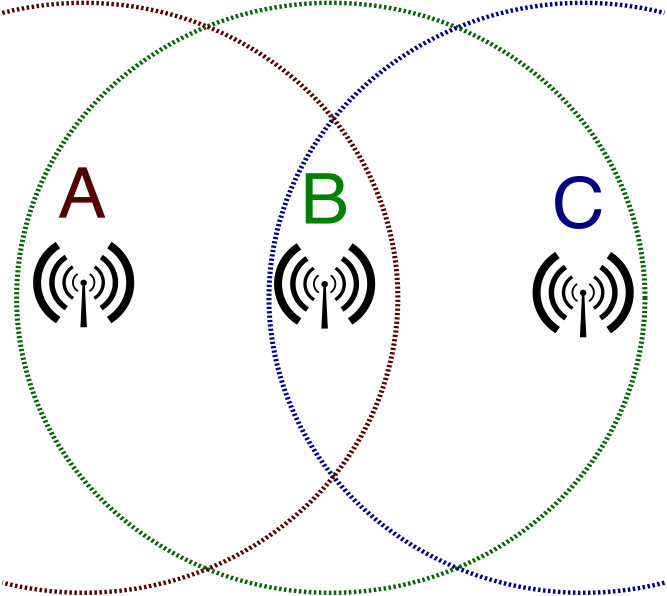
\includegraphics[keepaspectratio]{images/Wifi_hidden_station_problem.png}}
\caption{Fonte: Wikimedia Commons --- I nodi A e C non si trovano nel
reciproco raggio di copertura (cerchi tratteggiati non sovrapposti), ma
entrambi raggiungono B. Le trasmissioni simultanee causano una
collisione invisibile ai due mittenti.}
\end{figure}

La terza sfida è il \textbf{Multipath}: il segnale trasmesso non viaggia
solo in linea d'aria, ma si riflette, viene diffratto e disperso
(\emph{scattering}) dal suolo e dagli edifici circostanti. Al ricevitore
giungono quindi diverse copie del segnale originale, sfalsate
temporalmente. Per evitare che questi echi interferiscano con la
trasmissione successiva, i pacchetti di impulsi devono essere
distanziati nel tempo. L'intervallo minimo richiesto prima di poter
inviare un nuovo segnale senza sovrapposizioni si chiama \textbf{Tempo
di Coerenza} (\emph{Coherence Time} --- \(T_c\)). Il \(T_c\) è
inversamente proporzionale alla frequenza utilizzata e alla velocità del
ricevitore in caso di mobilità: sistemi ad alta frequenza e ricevitori
in movimento richiedono guardie temporali più brevi ma più frequenti.

\begin{figure}
\centering
\pandocbounded{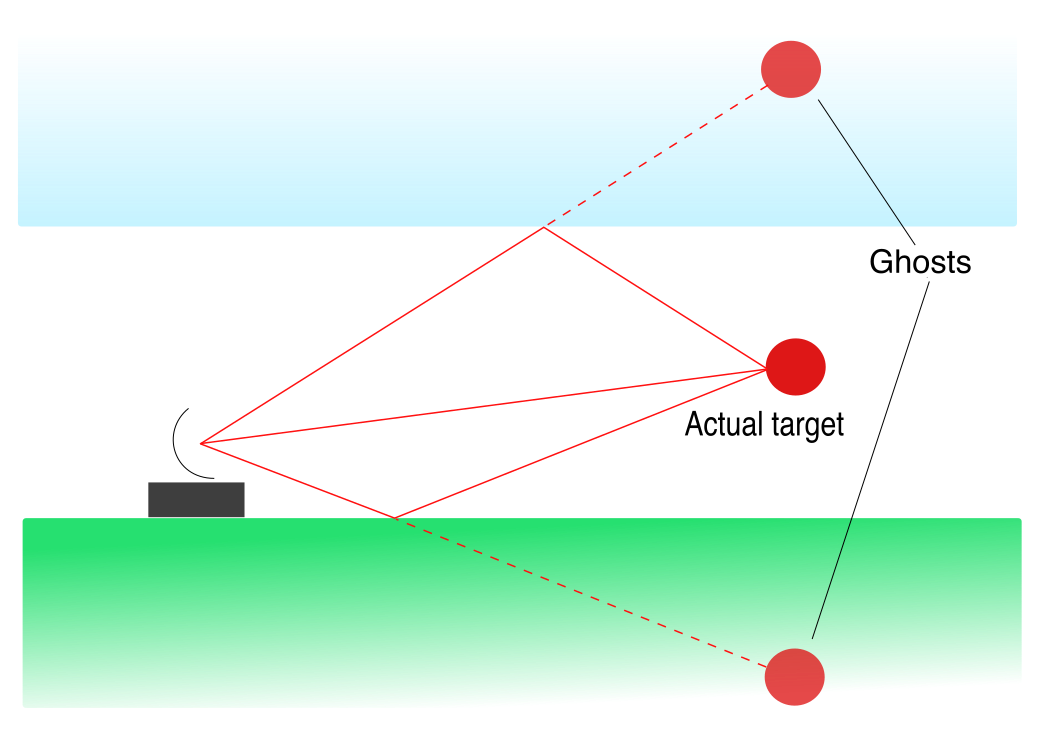
\includegraphics[keepaspectratio]{images/Multipath_propagation_diagram_en.png}}
\caption{Fonte: Wikimedia Commons --- Il trasmettitore (sinistra) invia
il segnale verso il ricevitore (destra) attraverso un percorso diretto e
più percorsi riflessi dagli edifici circostanti. Al ricevitore giungono
``fantasmi'' del segnale sfalsati nel tempo, che possono interferire con
la trasmissione successiva.}
\end{figure}

Questi tre fenomeni influenzano direttamente il \textbf{Bit Error Rate}
(\emph{BER}), ovvero la probabilità che un bit trasmesso arrivi errato.
Per un dato livello fisico, aumentare la potenza riduce il BER
incrementando l'SNR. L'adattamento dinamico dello schema di modulazione
in base all'SNR rilevato --- tecnica nota come \emph{Adaptive Modulation
and Coding} --- è uno dei meccanismi fondamentali dei sistemi wireless
moderni.

\begin{center}\rule{0.5\linewidth}{0.5pt}\end{center}

\section{Protocolli per Reti
Wireless}\label{protocolli-per-reti-wireless}

Le criticità fisiche descritte sopra creano sfide sistemiche che si
ripercuotono su tutti i livelli dello stack protocollare: visibilità
limitata della rete da parte del singolo nodo (terminali nascosti e
terminali esposti), fallimenti e mobilità dei terminali, limiti
intrinseci di batteria e memoria, e il problema della privacy causato
dall'intercettazione dei segnali (\emph{eavesdropping}).

Per mitigare questi limiti è necessario adottare meccanismi appositi. Il
\textbf{CSMA/CD}, protocollo standard per reti cablate Ethernet, non può
essere utilizzato: un nodo radio non è in grado di trasmettere e
ricevere contemporaneamente per ``ascoltare'' una collisione nel proprio
segnale. È quindi necessario un protocollo MAC alternativo. Serve
inoltre la gestione dell'\textbf{Hand-off} per la transizione tra Access
Point, e complessi protocolli di \textbf{Routing multi-hop} (per reti ad
hoc) capaci di reagire ai cambiamenti arbitrari della topologia di
vicinato (\emph{neighborhood}).

Nello stack dei protocolli per reti wireless, mentre i livelli
Applicazione e Trasporto (TCP/UDP) restano identici al mondo cablato, le
fondamenta si differenziano profondamente. Il livello di Rete per
ecosistemi senza infrastruttura si affida a protocolli speciali come
AODV, DSR o DYMO. Il livello Datalink implementa l'accesso al mezzo
tramite il protocollo \textbf{CSMA/CA} (\emph{Carrier Sense Multiple
Access with Collision Avoidance}), appositamente studiato per aggirare
le trappole dei collegamenti radio.

\newpage

\chapter{Protocolli MAC e Reti Wireless: Da CSMA/CD allo Standard IEEE
802.11}\label{protocolli-mac-e-reti-wireless-da-csmacd-allo-standard-ieee-802.11}

Questo capitolo esplora in modo approfondito l'evoluzione dei protocolli
di accesso al mezzo (MAC), partendo dalle fondamenta delle reti cablate
fino ad arrivare alle complesse dinamiche delle reti wireless.
Analizzeremo le sfide fisiche della trasmissione via radio, introducendo
i meccanismi architetturali e i protocolli, come il CSMA/CA e la
famiglia IEEE 802.11, che rendono possibile la connettività Wi-Fi
moderna.

\begin{center}\rule{0.5\linewidth}{0.5pt}\end{center}

\section{I Protocolli MAC per le Reti Cablate: Un
Riepilogo}\label{i-protocolli-mac-per-le-reti-cablate-un-riepilogo}

Per comprendere le reti wireless, è fondamentale fare un passo indietro
e analizzare le assunzioni di base che governano i protocolli MAC
(Medium Access Control) nelle tradizionali reti cablate. In questi
scenari, si assume generalmente che sia disponibile un \textbf{singolo
canale condiviso} per tutte le comunicazioni e che tutte le stazioni
collegate possano trasmettere e ricevere su di esso. Un principio
cardine è che se due o più frame vengono inviati simultaneamente, il
segnale risultante sul canale risulterà incomprensibile, generando
quella che viene definita una \textbf{collisione}. Nelle reti cablate,
tutte le stazioni sono fisicamente in grado di rilevare queste
collisioni. Nel tempo, sono stati sviluppati diversi protocolli per
gestire questo accesso, partendo da ALOHA e slotted ALOHA, fino ad
arrivare a CSMA e CSMA/CD.

\subsection{Il Protocollo CSMA/CD}\label{il-protocollo-csmacd}

Il protocollo \textbf{CSMA/CD} (Carrier Sense Multiple Access with
Collision Detection) si basa su un'idea fondamentale: ``ascoltare prima
di parlare''. Quando una stazione ha un frame pronto per l'invio, si
mette in ascolto sul canale per verificare se qualcun altro sta già
trasmettendo. Se il canale risulta occupato, la stazione attende
pazientemente che diventi libero (idle). Non appena il mezzo è libero,
la stazione inizia a trasmettere il suo frame. Se durante questa fase si
verifica una collisione, la stazione interrompe (aborts) immediatamente
la trasmissione, attende una quantità di tempo casuale e ripete l'intera
procedura.

\begin{calloutdefinition}{CSMA/CD — Carrier Sense Multiple Access with Collision Detection}

Protocollo di accesso al mezzo che combina l'ascolto preventivo del
canale (Carrier Sense) con il rilevamento attivo delle collisioni
durante la trasmissione (Collision Detection). Quando viene rilevata una
collisione, la trasmissione viene interrotta immediatamente, riducendo
lo spreco di banda. È il cuore dello standard IEEE 802.3 Ethernet.

\end{calloutdefinition}

Questo meccanismo di rilevamento precoce fa sì che, se due stazioni
percepiscono simultaneamente il canale libero e iniziano a trasmettere,
entrambe interrompano l'invio non appena rilevano la sovrapposizione dei
segnali, risparmiando così tempo prezioso e larghezza di banda. Per la
sua efficienza, il CSMA/CD è stato ampiamente adottato nei sottolivelli
MAC delle LAN, diventando il cuore dello standard \textbf{IEEE 802.3
Ethernet}.

\subsection{Limiti Temporali e Dimensione Minima del
Frame}\label{limiti-temporali-e-dimensione-minima-del-frame}

Il comportamento del CSMA/CD impone vincoli fisici ben precisi.
Definendo con \(T\) il tempo di propagazione necessario per raggiungere
la stazione più lontana della rete, nel caso peggiore occorrerà un tempo
pari al Round Trip Time (\(RTT\)), ovvero \(2T\), affinché la stazione
trasmittente possa rilevare con certezza una collisione.

\begin{itemize}
\item
  Ad esempio, se la stazione A inizia a trasmettere al tempo \(t=0\), e
  la stazione B (la più remota) inizia a trasmettere poco prima che il
  segnale di A la raggiunga (al tempo \(t=T-\delta\)), B rileverà la
  collisione quasi subito, al tempo \(t=T\).
\item
  Tuttavia, il fronte d'onda della collisione impiegherà un altro tempo
  \(T\) per viaggiare a ritroso verso A, che si accorgerà del problema
  solo al tempo \(t=2T-\delta\).
\end{itemize}

Di conseguenza, la stazione A deve obbligatoriamente monitorare il
canale per l'intero intervallo di tempo \(RTT\) con gli ``occhi aperti''
per intercettare eventuali interferenze. Una volta che l'intero frame è
stato inviato, infatti, la stazione mittente non ne conserva una copia
nel buffer MAC e non controlla più il mezzo trasmissivo per eventuali
collisioni. Per garantire che la trasmissione duri almeno quanto il
tempo \(RTT\), è necessario imporre un vincolo sulla \textbf{dimensione
minima del frame}.

Facciamo un esempio pratico: consideriamo una rete CSMA/CD con una
larghezza di banda di 10 Mbps e un tempo massimo di propagazione
(inclusi i ritardi hardware) di 25.6 \(\mu sec\). Nel caso peggiore, la
stazione deve trasmettere per un tempo di trasmissione minimo del frame
\(T_{fr} = 2 \times T_{p} = 51.2~\mu sec\) per poter intercettare con
successo una collisione. Traducendo questo tempo in dati, la dimensione
minima del frame risulta essere: 10 Mbps x 51.2 \(\mu sec\) =
\textbf{512 bit}, ovvero \textbf{64 byte} (la dimensione minima
effettiva adottata nell'Ethernet standard).

\subsection{Il Binary Exponential
Backoff}\label{il-binary-exponential-backoff}

Quando avviene una collisione, come si stabilisce il tempo di attesa
casuale? Il CSMA/CD utilizza l'algoritmo di \textbf{Binary Exponential
Backoff}. Il tempo successivo a una collisione viene suddiviso in
\emph{contention slots} (slot di contesa), la cui lunghezza è
esattamente pari al tempo di propagazione andata e ritorno nel caso
peggiore (\(2T\)).

\begin{itemize}
\item
  Dopo la prima collisione, ogni stazione coinvolta attende 0 oppure 1
  slot in modo casuale prima di riprovare.
\item
  Dopo la collisione iesima (\(i\)), la stazione sceglie un numero
  casuale \(x\) nell'intervallo \([0, 2^i - 1]\) e salta esattamente
  \(x\) slot prima di un nuovo tentativo.
\item
  Per evitare attese infinite in reti congestionate, dopo 10 collisioni
  consecutive l'intervallo di randomizzazione viene ``congelato'' a un
  massimo di 0..1023.
\item
  Se si raggiungono le 16 collisioni, il livello MAC si arrende e
  riporta il fallimento della trasmissione ai livelli superiori.
\end{itemize}

\begin{center}\rule{0.5\linewidth}{0.5pt}\end{center}

\section{Le Reti Wireless: Sfide e Problemi
Strutturali}\label{le-reti-wireless-sfide-e-problemi-strutturali}

Nelle reti cablate il rilevamento delle collisioni in fase di
trasmissione funziona perfettamente, ma nelle reti wireless questo
principio fallisce a causa della natura stessa del mezzo radio. Nelle
trasmissioni senza fili, la potenza del segnale decade rapidamente,
diminuendo in proporzione al quadrato della distanza.

A causa di questa attenuazione, il segnale emesso dall'antenna del
trasmettitore (il \emph{self-signal}) risulta infinitamente più forte
rispetto a qualsiasi altro segnale debole in arrivo da una stazione
distante. Questo ``acceca'' il trasmettitore, rendendogli impossibile
rilevare una collisione mentre sta inviando dati. Inoltre, le condizioni
del canale wireless sono spazialmente diverse tra chi trasmette e chi
riceve. Una collisione rilevata dal trasmettitore potrebbe non essere
una collisione al ricevitore, e viceversa. Nelle reti wireless, l'unica
cosa che conta veramente è l'\textbf{interferenza al ricevitore}, non al
mittente. Questa limitazione genera due problemi classici della
comunicazione radio: il \emph{Terminale Nascosto} e il \emph{Terminale
Esposto}.

\subsection{Il Problema del Terminale Nascosto (Hidden
Terminal)}\label{il-problema-del-terminale-nascosto-hidden-terminal}

\begin{calloutdefinition}{Terminale Nascosto (Hidden Terminal)}

Si verifica quando due o più stazioni, reciprocamente fuori dal raggio
radio l'una dell'altra, trasmettono simultaneamente verso un
destinatario comune. Poiché nessuna delle due stazioni riesce a rilevare
la trasmissione dell'altra, entrambe credono il canale libero e avviano
l'invio, causando una collisione al ricevitore che nessuna delle
sorgenti è in grado di percepire.

\end{calloutdefinition}

Immaginiamo quattro stazioni allineate: A, B, C e D. A è in raggio radio
con B; B è nel raggio di A e C; C è nel raggio di B e D. Supponiamo che
A stia attualmente trasmettendo dei dati a B. C, desiderando
trasmettere, si mette in ascolto sul mezzo. Poiché C si trova
fisicamente al di fuori del raggio di copertura radio di A, non
percepirà alcuna trasmissione in corso. Credendo che il canale sia
libero, C avvia una trasmissione (diretta a B o a D). Il risultato è
disastroso: i segnali di A e di C si sovrapporranno fisicamente in
corrispondenza dell'antenna di B, causando una collisione e distruggendo
i dati. In questo scenario, C è incapace di rilevare il potenziale
competitore (A) ed è quindi definito come \textbf{nascosto} (hidden)
rispetto alla comunicazione da A verso B. Il problema del terminale
nascosto si verifica quando due o più stazioni, reciprocamente fuori
raggio, trasmettono simultaneamente a un destinatario comune. Anche A,
per lo stesso motivo legato alla distanza, non si accorgerà della
collisione provocata da C.

\subsection{Il Problema del Terminale Esposto (Exposed
Terminal)}\label{il-problema-del-terminale-esposto-exposed-terminal}

\begin{calloutdefinition}{Terminale Esposto (Exposed Terminal)}

Si verifica quando una stazione rinuncia inutilmente a trasmettere
perché rileva sul canale il segnale di un'altra stazione, pur non
essendoci alcun rischio di collisione al ricevitore di destinazione. La
stazione ``esposta'' è in grado di ascoltare una trasmissione vicina ma
irrilevante, e ne viene erroneamente bloccata dall'invio di frame del
tutto legittimi verso un destinatario distante.

\end{calloutdefinition}

Consideriamo la stessa topologia (A, B, C, D). Questa volta, B sta
trasmettendo dati verso A, e parallelamente C desidera inviare un
messaggio a D. C, mettendosi in ascolto, rileva forte e chiaro il
segnale di B. Applicando ciecamente le regole del CSMA, C conclude
erroneamente di non poter trasmettere verso D, per paura di creare una
collisione. In realtà, se C iniziasse a trasmettere, il suo segnale
raggiungerebbe D senza problemi, e le due trasmissioni (da B verso A, e
da C verso D) potrebbero avvenire perfettamente in parallelo senza
disturbarsi a vicenda (le loro ``zone di interferenza'' ai ricevitori
non si sovrappongono in modo distruttivo). In questo caso, C è un
terminale \textbf{esposto} alla comunicazione tra B e A. Il problema del
terminale esposto impedisce a una stazione trasmittente di inviare frame
del tutto legittimi a causa dell'ascolto di un'interferenza locale
generata da un'altra stazione.

Il fatto che non si possa verificare lo stato del canale al ricevitore
semplicemente mettendosi in ascolto dal trasmettitore rende palese la
necessità di progettare protocolli MAC sensibilmente diversi da quelli
delle classiche reti LAN cablate.

\begin{center}\rule{0.5\linewidth}{0.5pt}\end{center}

\section{I Protocolli MACA e MACAW: Evitare le
Collisioni}\label{i-protocolli-maca-e-macaw-evitare-le-collisioni}

Per mitigare le problematiche descritte, nel 1990 Phil Karn presentò un
protocollo rivoluzionario chiamato \textbf{MACA} (Multiple Access with
Collision Avoidance), originariamente concepito per il ``packet radio''.
L'idea fondante del MACA non è quella di rilevare le collisioni, ma di
prevenirle stimolando il ricevitore a inviare un breve frame di
controllo prima che inizi la trasmissione dei dati veri e propri (molto
più lunghi). Le stazioni vicine, sentendo questo frame di controllo, si
asterranno dal trasmettere durante il successivo invio dei dati.

\subsection{Il Meccanismo RTS / CTS}\label{il-meccanismo-rts-cts}

Il funzionamento si basa su uno scambio di messaggi denominato RTS/CTS:

\begin{enumerate}
\def\labelenumi{\arabic{enumi}.}
\item
  \textbf{RTS (Request To Send):} Quando la stazione A desidera inviare
  dati a B, invia prima un breve pacchetto RTS indirizzato a B. Questo
  pacchetto non è generico, ma contiene l'ID della sorgente, l'ID della
  destinazione e, fattore cruciale, la lunghezza (durata) del frame dati
  che seguirà. Tutte le stazioni nel raggio di A (ad esempio C ed E)
  riceveranno questo RTS.
\item
  \textbf{CTS (Clear To Send):} Se B riceve l'RTS ed è pronto e
  desideroso di ricevere il messaggio, risponde trasmettendo un
  pacchetto CTS. Anche il CTS è un frame molto breve che copia e
  diffonde l'informazione sulla lunghezza dei dati ricevuta nell'RTS.
  Questo CTS verrà ascoltato da A (che ottiene così il permesso di
  procedere), ma anche da tutte le stazioni nel raggio di B (ad esempio
  D ed E).
\item
  Alla ricezione del frame CTS, la stazione A inizia a trasmettere il
  frame dati vero e proprio in totale sicurezza.
\end{enumerate}

\begin{callouttip}{Insight chiave del meccanismo RTS/CTS}

Il meccanismo RTS/CTS risolve entrambi i problemi topologici in modo
elegante: il terminale nascosto viene messo a tacere dal CTS del
ricevitore (che esso sente, anche se non ha sentito l'RTS del mittente),
mentre il terminale esposto viene liberato dall'obbligo di silenzio
perché sente l'RTS ma non il CTS (e quindi deduce che la ricezione
avviene fuori dalla sua area di influenza). Il canale viene così
``prenotato'' in modo distribuito, senza coordinamento centralizzato.

\end{callouttip}

Vediamo come il MACA risolve i problemi topologici precedenti:

\begin{itemize}
\item
  \textbf{Gestione dell'Esposto (C):} La stazione C ascolta l'RTS
  inviato da A, ma, essendo troppo lontana da B, non sentirà mai il
  relativo CTS. Deduce quindi di essere un terminale esposto, comprende
  che la ricezione avverrà lontano dalla sua area di influenza ed è
  quindi del tutto libera di iniziare una propria trasmissione.
\item
  \textbf{Gestione del Nascosto (D):} La stazione D non ascolta l'RTS di
  A, ma riceve forte e chiaro il CTS di risposta inviato da B. D capisce
  immediatamente che B è in procinto di ricevere dati e che una sua
  trasmissione disturberebbe B. Pertanto, D si silenzia
  disciplinatamente fino al completamento della trasmissione del frame
  dati (calcolando il tempo di attesa in base alla durata dichiarata nel
  CTS).
\item
  Se una stazione centrale come E ascolta sia l'RTS che il CTS, sa
  ovviamente di dover rimanere in silenzio per non disturbare la
  delicata operazione in corso.
\end{itemize}

Nel MACA, le collisioni possono ancora avvenire? Assolutamente sì, ma
\textbf{solo tra pacchetti RTS} (ad esempio se C e B inviano un RTS
simultaneamente verso A). Quando due RTS collidono, il destinatario non
genererà alcun CTS. Il grande vantaggio è che in queste collisioni non
viene perso alcun dato applicativo (NO DATA information is lost) e, dato
che gli RTS sono brevissimi (circa 20 byte), il canale viene tenuto
occupato e sprecato solo per una frazione di tempo minuscola. In caso di
collisione di RTS, i mittenti rinviano i messaggi utilizzando anch'essi
la tecnica del \textbf{Binary Exponential Backoff} mutuata
dall'Ethernet.

\subsection{L'Evoluzione: MACAW e l'Integrazione nel
CSMA/CA}\label{levoluzione-macaw-e-lintegrazione-nel-csmaca}

Il MACA originario è stato successivamente affinato dando vita al
protocollo \textbf{MACAW} (MACA for Wireless LANs), documentato da
Bharghavan et al.~nel 1994. Il MACAW ha introdotto miglioramenti
fondamentali:

\begin{itemize}
\item
  L'introduzione di un frame \textbf{ACK (Acknowledgement)} inviato dal
  ricevitore per confermare esplicitamente la ricezione corretta del
  frame dati.
\item
  Meccanismi di condivisione delle informazioni (come i contatori di
  backoff) tra le stazioni per garantire un'allocazione equa (fair) del
  throughput.
\end{itemize}

La combinazione dei concetti del MACAW con l'aggiunta di una fase
preventiva di ``Carrier Sensing'' (per evitare di inviare pacchetti RTS
inutili in un canale già visibilmente saturo) ha dato vita al protocollo
\textbf{CSMA/CA} (Carrier Sense Multiple Access with Collision
Avoidance), che è il cuore pulsante dello standard IEEE 802.11 moderno.

\subsection{Esercizio Pratico: Topologia di
Rete}\label{esercizio-pratico-topologia-di-rete}

Per testare la comprensione del meccanismo RTS/CTS, si consideri la
seguente topologia di rete a grafo: il nodo A è connesso a B e C; il
nodo D forma uno snodo centrale connesso a B, C, E, F; E è connesso a D
e F; F è connesso a D e E. Applicando le regole appena spiegate:

\begin{enumerate}
\def\labelenumi{\arabic{enumi}.}
\item
  In una trasmissione da E verso D, le stazioni B, C e F riceverebbero
  il CTS da D ma non l'RTS da E (agendo come terminali nascosti da
  proteggere).
\item
  Se D ascolta un RTS da E ma non il relativo CTS (ad esempio se E sta
  contattando F), D deduce di essere un terminale esposto rispetto a E.
\item
  Similmente, se B ascolta un CTS da D senza aver sentito alcun RTS,
  deve silenziarsi temporaneamente. Per esplorare appieno questi casi,
  gli studenti possono avvalersi delle simulazioni interattive per reti
  802.11 (con o senza terminali nascosti) fornite durante il corso.
\end{enumerate}

\begin{center}\rule{0.5\linewidth}{0.5pt}\end{center}

\section{Lo Standard IEEE 802.11 (Wi-Fi) e la sua
Architettura}\label{lo-standard-ieee-802.11-wi-fi-e-la-sua-architettura}

L'\textbf{IEEE} (Institute of Electrical and Electronics Engineers) è
l'ente principale a livello mondiale per la standardizzazione delle reti
locali (LAN). All'interno di questo ecosistema, il progetto IEEE 802 è
gestito dall'IEEE 802 Working Group. La filosofia architetturale prevede
che il sottolivello LLC (Logical Link Control) e i livelli superiori
(es. Rete/IP, Trasporto/TCP o UDP, Applicazione) rimangano comuni tra le
diverse tecnologie, mentre i livelli inferiori (il sottolivello MAC e il
livello Fisico) vengano specializzati in base al mezzo trasmissivo
adottato. Così come lo standard IEEE 802.3 definisce l'Ethernet CSMA/CD
su cavo (UTP, STP, fibra), la famiglia \textbf{IEEE 802.11} definisce lo
standard per le reti Wireless LAN (universalmente note con il marchio
commerciale \textbf{Wi-Fi}) che utilizzano la trasmissione radio. Altri
standard noti includono l'802.15 (Wireless PAN, come il Bluetooth) e
l'802.16 (Broadband wireless, WiMAX).

\subsection{L'Evoluzione della Famiglia
802.11}\label{levoluzione-della-famiglia-802.11}

Tutte le reti 802.11 operano sfruttando canali radio collocati nelle
bande \textbf{ISM} (Industrial, Scientific, and Medical) o
\textbf{U-NII} (Unlicensed National Information Infrastructure),
comunemente nelle frequenze dei 900 MHz, 2.4 GHz e 5 GHz, garantendo
progressivamente decine fino a migliaia di Mbit/s di capacità.
Ripercorriamo l'evoluzione storica del livello fisico (PHY):

\begin{itemize}
\item
  \textbf{IEEE 802.11 (Legacy mode):} Rilasciato originariamente nel
  1997 e chiarito nel 1999. Operava nella banda dei 2.4 GHz offrendo
  data rate molto bassi (1-2 Mbps) implementati tramite raggi infrarossi
  (IR) o frequenze radio. Avendo troppi gradi di libertà implementativi,
  poneva severi problemi di interoperabilità ed è oggi considerato
  obsoleto.
\item
  \textbf{IEEE 802.11a:} Rilasciato nel 1999, è stato pioniere dell'uso
  della banda a 5 GHz (U-NII), offrendo un throughput tipico di 23 Mbps
  e un tetto massimo di 54 Mbps.
\item
  \textbf{IEEE 802.11b:} Contemporaneo alla versione `a' (1999), divenne
  lo standard di massa iniziale. Operando a 2.4 GHz (massimo 11 Mbps),
  implementava schemi di modulazione specifici per limitare le forti
  interferenze in quella banda affollata (telefoni cordless, microonde,
  ecc.).
\item
  \textbf{IEEE 802.11g:} Introdotto nel 2003, mantenne l'uso della banda
  a 2.4 GHz ma aumentò la velocità fino a 54 Mbps.
\item
  \textbf{IEEE 802.11n (WiFi 4):} Rilasciato nel 2009, ha introdotto il
  rivoluzionario supporto alla tecnologia \textbf{MIMO} (multiple-input
  multiple-output). Usando più antenne in trasmissione e ricezione
  contemporaneamente sia a 2.4 GHz che a 5 GHz, ha spinto il data rate
  massimo fino a 248 Mbps (e teoricamente 600 Mbps) estendendo la
  portata.
\item
  \textbf{IEEE 802.11ac (WiFi 5):} Standardizzato nel 2013, si concentra
  esclusivamente sui 5 GHz, superando la barriera del gigabit (fino a
  1.3 Gbps per flussi base, fino a 3.47 Gbps massimi).
\item
  \textbf{IEEE 802.11ax (WiFi 6):} Rilasciato intorno al 2019/2020,
  supporta 2.4 GHz, 5 GHz e introduce i 6 GHz. Progettato per efficienza
  estrema in ambienti densi, raggiunge fino a 10-14 Gbps, con sensibili
  miglioramenti nel consumo energetico dei dispositivi e nei protocolli
  di sicurezza.
\item
  \emph{(Menzioni speciali):} Versioni come 802.11af (2014, che sfrutta
  le bande TV inutilizzate) e 802.11ah (2017, per applicazioni a 900 MHz
  a lunghissimo raggio fino a 1 Km) si rivolgono ad ambiti specialistici
  o all'IoT.
\end{itemize}

{\def\LTcaptype{none} % do not increment counter
\begin{longtable}[]{@{}
  >{\raggedright\arraybackslash}p{(\linewidth - 8\tabcolsep) * \real{0.2000}}
  >{\raggedright\arraybackslash}p{(\linewidth - 8\tabcolsep) * \real{0.2000}}
  >{\raggedright\arraybackslash}p{(\linewidth - 8\tabcolsep) * \real{0.2000}}
  >{\raggedright\arraybackslash}p{(\linewidth - 8\tabcolsep) * \real{0.2000}}
  >{\raggedright\arraybackslash}p{(\linewidth - 8\tabcolsep) * \real{0.2000}}@{}}
\toprule\noalign{}
\begin{minipage}[b]{\linewidth}\raggedright
\textbf{Standard}
\end{minipage} & \begin{minipage}[b]{\linewidth}\raggedright
\textbf{Anno}
\end{minipage} & \begin{minipage}[b]{\linewidth}\raggedright
\textbf{Max Data Rate}
\end{minipage} & \begin{minipage}[b]{\linewidth}\raggedright
\textbf{Copertura (Range)}
\end{minipage} & \begin{minipage}[b]{\linewidth}\raggedright
\textbf{Frequenza}
\end{minipage} \\
\midrule\noalign{}
\endhead
\bottomrule\noalign{}
\endlastfoot
\textbf{802.11b} & 1999 & 11 Mbps & 30 m & 2.4 GHz \\
\textbf{802.11g} & 2003 & 54 Mbps & 30 m & 2.4 GHz \\
\textbf{802.11n (WiFi 4)} & 2009 & 600 Mbps & 70 m & 2.4, 5 GHz \\
\textbf{802.11ac (WiFi 5)} & 2013 & 3.47 Gbps & 70 m & 5 GHz \\
\textbf{802.11ax (WiFi 6)} & 2020 & 14 Gbps & 70 m & 2.4, 5 GHz \\
\textbf{802.11af} & 2014 & 35-560 Mbps & 1 Km & Bande TV (54-790 MHz) \\
\textbf{802.11ah} & 2017 & 347 Mbps & 1 Km & 900 MHz \\
Tabella riassuntiva delle specifiche IEEE 802.11. Tutti utilizzano
CSMA/CA e supportano configurazioni base-station o reti ad-hoc. & & &
& \\
\end{longtable}
}

\subsection{Elementi Architetturali: BSS ed
ESS}\label{elementi-architetturali-bss-ed-ess}

Dal punto di vista della struttura della rete, il blocco logico
fondamentale dell'802.11 è il \textbf{BSS (Basic Service Set)}. Un BSS è
semplicemente un gruppo di stazioni wireless in grado di comunicare tra
loro sotto il controllo di una singola funzione di coordinamento.
Esistono due modalità operative principali per un BSS:

\begin{enumerate}
\def\labelenumi{\arabic{enumi}.}
\item
  \textbf{Rete Ad-Hoc:} L'infrastruttura di controllo è assente. Le
  stazioni comunicano direttamente e pariteticamente (peer-to-peer)
  l'una con l'altra.
\item
  \textbf{Rete Infrastrutturata:} È presente una stazione base
  specializzata chiamata \textbf{AP (Access Point)}. Tutte le
  comunicazioni, anche tra due host della stessa cella, vengono
  obbligatoriamente incanalate e gestite attraverso l'AP.
\end{enumerate}

Per formare reti più vaste, più BSS vengono interconnessi tra loro
creando un \textbf{ESS (Extended Service Set)}. In questo scenario, gli
Access Point fungono da ponti e forniscono connettività inter-cella
instradando il traffico attraverso un'infrastruttura fissa (solitamente
cablata) denominata \textbf{DS (Distribution System)}.

\subsection{Selezione del Canale e Meccanismi di
Associazione}\label{selezione-del-canale-e-meccanismi-di-associazione}

Lo spettro radio assegnato al Wi-Fi è logicamente suddiviso in vari
canali operanti a frequenze leggermente diverse. L'amministratore di
rete configura manualmente o automaticamente la frequenza in cui opera
un determinato AP. Un problema tipico di progettazione si verifica
quando AP limitrofi (vicini fisicamente) vengono configurati sullo
stesso canale, generando interferenze distruttive tra le celle.

Quando un dispositivo wireless (es. smartphone o laptop) arriva in
un'area coperta, deve associarsi a un AP prima di poter navigare. Questo
avviene tramite una fase di scansione dei canali (scansione alla ricerca
della rete e del suo \textbf{SSID} - Service Set Identifier, oltre
all'indirizzo MAC dell'AP noto come BSSID). Esistono due modalità di
scansione:

\begin{enumerate}
\def\labelenumi{\arabic{enumi}.}
\item
  \textbf{Scansione Passiva (Passive Scanning):} L'host si mette in
  ascolto silente dei \emph{beacon frames} periodicamente e
  automaticamente trasmessi dagli AP circostanti. Una volta ricevuti i
  beacon, l'host sceglie tipicamente l'AP il cui segnale arriva con la
  massima potenza (highest signal strength). A questo punto, l'host
  invia all'AP selezionato un frame di \emph{Association Request}, e
  attende in risposta un frame di \emph{Association Response}.
\item
  \textbf{Scansione Attiva (Active Scanning):} L'host assume
  l'iniziativa e invia attivamente in broadcast un \emph{Probe Request
  frame} su vari canali. Gli AP nel raggio d'azione che ricevono la
  richiesta rispondono con \emph{Probe Response frames}. L'host valuta
  le risposte, sceglie l'AP e avvia il classico handshake inviando l'
  \emph{Association Request} e ricevendo la \emph{Association Response}.
\end{enumerate}

Completata l'associazione, la stazione segue tipicamente le normali
procedure di autenticazione di sicurezza e avvia un client DHCP per
ottenere un indirizzo IP valido nella sottorete gestita dall'AP.

\begin{center}\rule{0.5\linewidth}{0.5pt}\end{center}

\section{Il Sottolivello MAC 802.11: DCF, PCF e Dinamiche
CSMA/CA}\label{il-sottolivello-mac-802.11-dcf-pcf-e-dinamiche-csmaca}

Il sottolivello MAC dello standard IEEE 802.11 è diviso in due funzioni
architetturali ben distinte che determinano le modalità di accesso al
mezzo: la DCF e la PCF.

\begin{itemize}
\item
  \textbf{PCF (Point Coordination Function):} È un modulo opzionale che
  si posiziona concettualmente ``sopra'' il livello DCF e gestisce
  servizi \emph{contention-free} (ovvero privi di collisioni) in modo
  centralizzato, controllando rigorosamente i turni di trasmissione
  degli host.
\item
  \textbf{DCF (Distributed Coordination Function):} È il fondamento
  universale del MAC 802.11. È sempre disponibile in ogni rete (ad-hoc o
  infrastrutturata) e gestisce l'accesso \emph{contention-based} tramite
  il protocollo \textbf{CSMA/CA}. Essendo un sistema decentralizzato e
  distribuito, le collisioni sono ovviamente una possibilità reale.
\end{itemize}

\subsection{Il Carrier Sensing: Fisico e Virtuale
(NAV)}\label{il-carrier-sensing-fisico-e-virtuale-nav}

Nel CSMA/CA, prima di trasmettere, una stazione deve necessariamente
accertarsi che il canale sia libero eseguendo il \textbf{Carrier
Sensing}. Questo avviene su due livelli interconnessi:

\begin{enumerate}
\def\labelenumi{\arabic{enumi}.}
\item
  \textbf{Sensore Fisico (Physical CS):} L'hardware analizza la
  frequenza per rilevare energia o intercettare l'arrivo di un segnale
  elettromagnetico, stabilendo se c'è attività nel canale dovuta ad
  altre fonti.
\item
  \textbf{Sensore Virtuale (Virtual CS):} È il meccanismo logico
  software. Il protocollo prevede l'inserimento di precise informazioni
  sulla durata temporale della comunicazione nell'header dei primissimi
  byte di frame come RTS, CTS e pacchetti Dati generici. Ascoltando
  queste durate, ogni stazione aggiorna una variabile locale chiamata
  \textbf{NAV} (Network Allocation Vector). Il NAV funge da timer:
  indica al sistema per quanto tempo il canale sarà ``virtualmente
  occupato'' e quanto bisogna aspettare prima di poter persino pensare
  di campionare nuovamente lo stato fisico del mezzo.
\end{enumerate}

Basta che uno solo dei due sensori (Fisico o Virtuale/NAV) dia esito
``occupato'', affinché la stazione consideri l'intero canale
indisponibile (busy).

\subsection{Gli Interframe Spaces (IFS) e le
Priorità}\label{gli-interframe-spaces-ifs-e-le-priorituxe0}

Nel mondo 802.11, il concetto di ``canale libero'' è strettamente legato
ai tempi. L'accesso prioritario al mezzo è regolamentato imponendo l'uso
di periodi obbligatori di attesa e inattività chiamati \textbf{IFS}
(Interframe Space). Lo standard definisce durate precise:

\begin{itemize}
\item
  \textbf{DIFS (Distributed IFS):} È un intervallo temporale ``lungo''.
  È il tempo minimo di default che una stazione normale deve attendere
  (misurando canale ininterrottamente libero) prima di poter avviare una
  trasmissione regolare.
\item
  \textbf{SIFS (Short IFS):} È un intervallo temporale ``brevissimo''.
  Viene utilizzato esclusivamente come tempo di attesa prima di inviare
  pacchetti critici e ad altissima priorità, come i CTS o i messaggi di
  conferma ACK. Poiché rigorosamente \textbf{SIFS \textless{} DIFS}, la
  stazione che sta completando un handshake (es. sta per inviare un ACK)
  riuscirà sempre a prendere possesso del canale prima che le altre
  stazioni in attesa finiscano di contare il proprio lungo periodo DIFS,
  garantendo l'assenza di interruzioni durante le transazioni.
\end{itemize}

\subsection{L'Algoritmo CSMA/CA in
Azione}\label{lalgoritmo-csmaca-in-azione}

Sintetizziamo i passaggi della DCF per trasmettitore e ricevitore:

\begin{enumerate}
\def\labelenumi{\arabic{enumi}.}
\item
  \textbf{Attesa Iniziale:} Se la stazione mittente percepisce il canale
  costantemente libero per un periodo pari almeno al DIFS, trasmette
  l'intero frame dati (ricordiamo, senza collision detection).
\item
  \textbf{Backoff Randomico:} Se invece il canale risulta occupato
  (fisicamente o tramite NAV), la stazione fa partire un tempo di
  backoff casuale. Questo timer scorre alla rovescia (counts down)
  solamente mentre il canale risulta libero; si congela istantaneamente
  se un'altra stazione inizia a trasmettere. Quando il timer raggiunge
  lo zero (ed è trascorso anche il DIFS), la stazione trasmette.
\item
  \textbf{Il ruolo dell'ACK:} Ricevuto correttamente un frame, il
  destinatario attende il breve tempo SIFS e risponde immediatamente con
  un pacchetto ACK per confermare l'avvenuto recapito (l'ACK è vitale in
  wireless a causa delle perdite naturali e dei terminali nascosti).
\item
  \textbf{Gestione delle Collisioni:} Cosa succede se l'ACK non arriva?
  Il mittente assume che si sia verificata una collisione (o una perdita
  per attenuazione). Si innesca la penalità: il mittente incrementa
  l'intervallo casuale di backoff (raddoppiandolo ad ogni tentativo
  fallito secondo la logica Binary Exponential Backoff), aspetta il DIFS
  e ritenta la procedura.
\end{enumerate}

\emph{Nota sull'inefficienza delle collisioni semplici:} Se avviene una
collisione e l'RTS/CTS non viene impiegato, poiché nessuna stazione è in
grado di interrompere la trasmissione a metà, l'intero frame dati verrà
completamente sprecato, ``sprecando'' una massiccia porzione di
larghezza di banda, specialmente se il frame era molto grande.

\subsection{RTS e CTS nello Standard IEEE
802.11}\label{rts-e-cts-nello-standard-ieee-802.11}

Per evitare l'enorme spreco di risorse causato dalle collisioni sui
frame dati primari, l'implementazione 802.11 permette di ``prenotare''
(reserve) il mezzo trasmissivo utilizzando i mini-pacchetti RTS e CTS
(descritti nel MACA). L'host invia prima l'RTS in modalità CSMA; l'AP di
destinazione diffonde in broadcast un CTS per notificare
l'autorizzazione e zittire tutte le altre stazioni (che aggiornano il
loro NAV), permettendo poi la trasmissione incontrastata dei dati. Anche
qui, se due RTS collidono per il possesso (reservation collision), solo
i pacchettini corti vanno persi.

Gli amministratori di rete possono configurare la modalità DCF per
gestire l'RTS/CTS in tre modi differenti (RTS Threshold):

\begin{enumerate}
\def\labelenumi{\arabic{enumi}.}
\item
  \textbf{Mai (Never):} Non si usano RTS/CTS. Questa impostazione è
  eccellente per reti con carico di traffico estremamente leggero, in
  cui il ritardo aggiunto dallo scambio RTS/CTS sarebbe inutile e
  inefficiente.
\item
  \textbf{Soglia di dimensione:} RTS/CTS viene abilitato unicamente per
  messaggi ``lunghi'', ovvero quando la dimensione del pacchetto supera
  un certo limite (RTS Threshold) calcolato dall'amministratore.
\item
  \textbf{Sempre (Always):} L'uso dell'RTS/CTS è imposto per ogni
  trasmissione. È l'impostazione raccomandata in condizioni di altissimo
  carico e densità sul mezzo wireless per minimizzare le disastrose
  probabilità di sovrapposizione e la gestione dei nodi nascosti.
\end{enumerate}

\begin{center}\rule{0.5\linewidth}{0.5pt}\end{center}

\begin{calloutnote}{Riepilogo dei Concetti Chiave}

Nelle LAN cablate (802.3) il rilevamento delle collisioni avviene
direttamente durante la trasmissione (CSMA/CD), bloccando
tempestivamente l'invio. Nelle WLAN (802.11) questo è fisicamente
precluso a causa dell'attenuazione del segnale radio, per cui si
adottano tecniche di ``Avoidance'' preventivo basate su ACK obbligatori
(CSMA/CA). I problemi strutturali del mezzo radio --- terminale nascosto
ed esposto --- derivano dall'impossibilità di verificare lo stato del
canale al ricevitore ascoltando dal trasmettitore; entrambi vengono
gestiti tramite il meccanismo di prenotazione del canale MACA/MACAW
integrato nello standard 802.11 attraverso lo scambio RTS/CTS. Il
Virtual Carrier Sensing e il NAV garantiscono il blocco totale delle
trasmissioni indesiderate attraverso timer logici interni che propagano
in modo distribuito la durata delle comunicazioni in corso.
L'architettura unificata dello standard IEEE 802.11 --- basata su BSS e
ESS, tempi di attesa differenziati (SIFS vs DIFS) e Backoff Esponenziale
--- opera sulle bande ISM/U-NII libere da licenze, consentendo la
connettività Wi-Fi moderna in una vasta gamma di scenari, dalle reti
ad-hoc alle infrastrutture enterprise.

\end{calloutnote}

\newpage

\chapter{Mobile Networks: dalle reti cellulari al
4G/5G}\label{mobile-networks-dalle-reti-cellulari-al-4g5g}

Questa lezione introduce i fondamenti dell'architettura delle reti
cellulari moderne, ripercorrendo l'evoluzione storica dal 1G fino al 5G
e proiettandosi verso il 6G. Il filo conduttore è capire come ogni
generazione abbia trasformato non solo la velocità di trasmissione, ma
soprattutto il modello architetturale: dalla commutazione a circuito
puramente analogica del 1G, alla \textbf{all-IP core} del 4G LTE, fino
alla \textbf{Service Based Architecture} cloud-native del 5G. Lungo
questo percorso emergono i meccanismi che rendono le reti cellulari
peculiari rispetto a Internet cablata: la mobilità come servizio nativo
di prima classe, il tunneling per preservare gli indirizzi IP durante
gli spostamenti, l'autenticazione mutua basata sulla SIM e la
separazione netta tra piano di controllo e piano dati.

\begin{calloutnote}{Riferimenti bibliografici}

Le slide sono un libero adattamento del libro \textbf{``Computer
Networking: A Top-Down Approach''} (8ª edizione, 2020) di \textbf{James
F. Kurose} e \textbf{Keith W. Ross}. Per l'architettura 5G il
riferimento è \textbf{``5G Mobile Networks: A Systems Approach''} di
\textbf{Larry Peterson} e \textbf{Oguz Sunay} (CC BY-NC-ND 4.0). Il
quadro evolutivo verso il 6G riprende: Zakria Qadir et al.,
\emph{``Towards 6G Internet of Things: Recent advances, use cases, and
open challenges''}, ICT Express, Elsevier, Giugno 2023.

\end{calloutnote}

\begin{center}\rule{0.5\linewidth}{0.5pt}\end{center}

\section{L'evoluzione delle reti cellulari: dal 1G al
6G}\label{levoluzione-delle-reti-cellulari-dal-1g-al-6g}

Le reti cellulari hanno attraversato in quattro decenni una
trasformazione che le ha portate da semplici sistemi di telefonia
analogica a infrastrutture distribuite per l'Internet of Things globale.
Ogni ``generazione'' non rappresenta solo un salto di velocità ma un
ripensamento dell'architettura.

Il \textbf{1G} degli anni '80 (standard AMPS, TACS) trasportava solo
voce in formato analogico, multiplexato in frequenza (FDMA), con
copertura e sicurezza molto limitate. Negli anni '90 il \textbf{2G}
introduce la voce digitale (GSM, CDMA) con multiplexing combinato
TDM+FDM e gli SMS; con l'estensione \textbf{2.5G/GPRS} (General Packet
Radio Service) si affaccia per la prima volta il concetto di
\textbf{commutazione a pacchetto per i dati}, accanto alla commutazione
a circuito che continua a gestire la voce. Il \textbf{3G} degli anni
2000 (UMTS, CDMA2000, HSPDA) porta l'accesso Web in mobilità: la rete
voce resta a circuito ma in parallelo opera una rete dati a pacchetto.

La svolta architetturale arriva con il \textbf{4G} (LTE Advanced, anni
2010): tutto il traffico --- voce inclusa --- viaggia su un
\textbf{All-IP core}, tunnelizzato come pacchetti IP dalla Base Station
al gateway. Cade la separazione fra rete voce e rete dati e si introduce
la separazione fra piano di controllo e piano dati. Il \textbf{5G} degli
anni 2020 (5G NR) ridisegna il core in chiave cloud-native
(\textbf{Service Based Architecture}), introduce il \textbf{network
slicing} per partizionare logicamente la rete, e sfrutta sia frequenze
sub-6 GHz sia onde millimetriche (mmWave). Il \textbf{6G}, atteso
intorno al 2030, è già oggetto di ricerca e punta a un ecosistema
``fully-connected'' potenziato da AI con architetture \emph{cell-less}.

{\def\LTcaptype{none} % do not increment counter
\begin{longtable}[]{@{}
  >{\raggedright\arraybackslash}p{(\linewidth - 14\tabcolsep) * \real{0.1250}}
  >{\raggedright\arraybackslash}p{(\linewidth - 14\tabcolsep) * \real{0.1250}}
  >{\raggedright\arraybackslash}p{(\linewidth - 14\tabcolsep) * \real{0.1250}}
  >{\raggedright\arraybackslash}p{(\linewidth - 14\tabcolsep) * \real{0.1250}}
  >{\raggedright\arraybackslash}p{(\linewidth - 14\tabcolsep) * \real{0.1250}}
  >{\raggedright\arraybackslash}p{(\linewidth - 14\tabcolsep) * \real{0.1250}}
  >{\raggedright\arraybackslash}p{(\linewidth - 14\tabcolsep) * \real{0.1250}}
  >{\raggedright\arraybackslash}p{(\linewidth - 14\tabcolsep) * \real{0.1250}}@{}}
\toprule\noalign{}
\begin{minipage}[b]{\linewidth}\raggedright
Gen
\end{minipage} & \begin{minipage}[b]{\linewidth}\raggedright
Anni
\end{minipage} & \begin{minipage}[b]{\linewidth}\raggedright
Standard
\end{minipage} & \begin{minipage}[b]{\linewidth}\raggedright
Velocità
\end{minipage} & \begin{minipage}[b]{\linewidth}\raggedright
Accesso
\end{minipage} & \begin{minipage}[b]{\linewidth}\raggedright
Voice switch
\end{minipage} & \begin{minipage}[b]{\linewidth}\raggedright
Data switch
\end{minipage} & \begin{minipage}[b]{\linewidth}\raggedright
Caratteristiche
\end{minipage} \\
\midrule\noalign{}
\endhead
\bottomrule\noalign{}
\endlastfoot
\textbf{1G} & 1980s & AMPS, TACS & 2.4 kbps & FDMA & Circuit & Circuit &
Voce analogica, copertura limitata \\
\textbf{2G} & 1990s & GSM, CDMA, EDGE & 64 kbps & TDM+FDM & Circuit &
Circuit & Voce digitale + SMS \\
\textbf{2.5G} & fine '90s & GPRS & --- & --- & Circuit & Packet & Prima
commutazione a pacchetto sui dati \\
\textbf{3G} & 2000s & UMTS, CDMA2000, HSPDA & fino a 2 Mbps & CDMA &
Circuit & Packet & Web in mobilità \\
\textbf{4G} & 2010s & LTE Advanced & 100--1000 Mbps & OFDMA & Packet &
Packet & All-IP core, tunneling, separazione control/data \\
\textbf{5G} & 2020s & 5G NR & fino a \textasciitilde20 Gbps & OFDMA +
mmWave & Packet & Packet & SBA, network slicing, sub-6 GHz + mmWave \\
\textbf{6G} & 2030s (prev.) & --- & \textasciitilde1 Tbps & --- & --- &
--- & Cell-less, AI-native, fully-connected \\
\end{longtable}
}

\begin{callouttip}{La traiettoria di fondo}

A ogni generazione la rete diventa più simile a Internet: prima si
introduce la commutazione a pacchetto sui dati (2.5G), poi anche sulla
voce (4G), poi si modularizza il core in microservizi (5G). La direzione
è quella di una rete cellulare \textbf{indistinguibile da un cloud
distribuito}, dove la mobilità è una feature applicativa e non
un'eccezione.

\end{callouttip}

\begin{center}\rule{0.5\linewidth}{0.5pt}\end{center}

\section{Diffusione e standardizzazione delle reti
4G/5G}\label{diffusione-e-standardizzazione-delle-reti-4g5g}

Le reti 4G/5G sono oggi la soluzione standard per l'Internet mobile su
area geografica ampia. Già nel 2019 i dispositivi connessi via banda
larga mobile superavano quelli a banda larga fissa con un rapporto di
\textbf{5 a 1}. La disponibilità del 4G ha raggiunto il \textbf{97\% del
tempo in Corea} e il \textbf{90\% negli Stati Uniti}, con velocità
tipiche di \textbf{20 Mbps e oltre}. La standardizzazione tecnica è
curata dal consorzio \textbf{3GPP} (3rd Generation Partnership Project),
che definisce in particolare lo standard \textbf{LTE (Long-Term
Evolution)} per il 4G e il \textbf{5G NR (New Radio)} per il 5G.

\begin{center}\rule{0.5\linewidth}{0.5pt}\end{center}

\section{Architettura di alto livello: RAN, Backhaul, Mobile
Core}\label{architettura-di-alto-livello-ran-backhaul-mobile-core}

L'architettura di una rete cellulare 4G/5G si scompone in tre blocchi
funzionali che collaborano per portare un pacchetto IP dal dispositivo
dell'utente fino a Internet (e viceversa):

\begin{itemize}
\tightlist
\item
  \textbf{Radio Access Network (RAN)} --- è la ``rete d'accesso'' radio:
  una collezione distribuita di \textbf{Base Station} (stazioni base)
  che gestiscono lo spettro radio condiviso fra i dispositivi
  all'interno della loro \textbf{cella} di copertura.
\item
  \textbf{Backhaul Network} --- interconnette la RAN con il Mobile Core.
  Tipicamente cablata in fibra ottica, ma sono in arrivo soluzioni
  wireless integrate (Integrated Access Backhaul, IAB).
\item
  \textbf{Mobile Core Network} --- fornisce connettività IP per dati e
  voce, garantisce i requisiti di \textbf{QoS}, traccia la mobilità per
  assicurare un servizio ininterrotto e gestisce billing \& charging. Si
  chiama \textbf{Evolved Packet Core (EPC)} in 4G e \textbf{NG-Core} in
  5G.
\end{itemize}

\begin{figure}
\centering
\pandocbounded{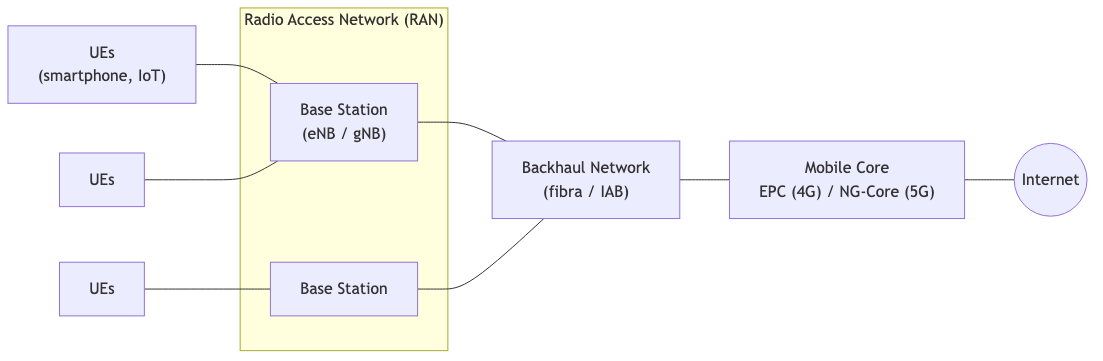
\includegraphics[keepaspectratio]{images/mermaid-lezione-7-lab-mobile-networks-01.png}}
\caption{I tre blocchi dell'architettura cellulare. La RAN gestisce lo
spettro, il backhaul è il ``trasporto'' verso l'interno della rete, il
Mobile Core fa da gateway verso Internet e custodisce le funzioni di
mobilità, autenticazione e charging.}
\end{figure}

\begin{center}\rule{0.5\linewidth}{0.5pt}\end{center}

\section{Gli elementi dell'architettura 4G
LTE}\label{gli-elementi-dellarchitettura-4g-lte}

L'architettura 4G LTE è comunemente chiamata \textbf{all-IP Enhanced
Packet Core (EPC)}. Vale la pena entrare nel dettaglio dei suoi
componenti, perché molti concetti sopravvivono inalterati anche in 5G
(cambiando solo nome o granularità).

\subsection{User Equipment (UE)}\label{user-equipment-ue}

\begin{calloutdefinition}{UE — User Equipment}

Con \textbf{UE} si intende qualsiasi dispositivo terminale dotato di
radio 4G LTE: smartphone, tablet, laptop, dispositivo IoT. Implementa
l'\textbf{intero stack Internet a 5 livelli}. La sua identità globale è
l'\textbf{IMSI} (International Mobile Subscriber Identity), un codice a
64 bit memorizzato sulla \textbf{SIM} (Subscriber Identity Module).
L'IMSI identifica univocamente l'abbonato nel sistema cellulare
mondiale, codificando la nazione e il carrier ``home''.

\end{calloutdefinition}

\subsection{Base Station (eNode-B)}\label{base-station-enode-b}

La Base Station si trova al ``margine'' (\emph{edge}) della rete del
carrier: gestisce le risorse radio wireless e i dispositivi all'interno
della propria \textbf{cella}, e coordina l'autenticazione del
dispositivo interfacciandosi con gli altri elementi del core. Rispetto a
un Access Point Wi-Fi, però, il suo ruolo è molto più attivo:

\begin{itemize}
\tightlist
\item
  coordina gli \textbf{handover} del dispositivo tra celle adiacenti,
  mantenendo le sessioni in corso;
\item
  collabora con le Base Station vicine per \textbf{minimizzare le
  interferenze radio};
\item
  crea \textbf{tunnel IP specifici per ogni dispositivo} verso i gateway
  del core;
\item
  gestisce direttamente la mobilità intercella.
\end{itemize}

In gergo LTE è chiamata \textbf{eNode-B} (evolved NodeB).

\subsection{Mobility Management Entity
(MME)}\label{mobility-management-entity-mme}

L'MME è il ``cervello'' del piano di controllo. Coordina
l'\textbf{autenticazione bidirezionale} (dispositivo → rete e rete →
dispositivo) interfacciandosi con l'HSS della rete \emph{home}
dell'utente. Si occupa inoltre della gestione del dispositivo:
\textbf{handover} fra celle, \textbf{tracking/paging} della posizione, e
setup dei percorsi (tunneling) verso S-GW e P-GW.

\subsection{Home Subscriber Service
(HSS)}\label{home-subscriber-service-hss}

\begin{calloutdefinition}{HSS — Home Subscriber Service}

Database centrale che contiene tutte le informazioni sugli abbonati.
Memorizza i dati dei dispositivi per i quali la rete in cui si trova
l'HSS è la \textbf{home network} (``rete di casa''), e collabora
strettamente con l'MME nelle procedure di autenticazione.

\end{calloutdefinition}

\subsection{Serving Gateway (S-GW)}\label{serving-gateway-s-gw}

L'S-GW si trova \textbf{sul percorso dei dati} fra dispositivo mobile e
Internet. Si occupa dell'inoltro dei pacchetti IP da/verso la RAN e
funge da \textbf{Local Mobility Anchor}: quando un utente si sposta da
un eNode-B a un altro all'interno della stessa rete, l'S-GW fa da
``ancora locale'' della sessione, cosicché l'handover risulti
trasparente ai livelli superiori.

\subsection{PDN Gateway (P-GW)}\label{pdn-gateway-p-gw}

Il \textbf{Packet Data Network Gateway} connette il core 4G alle reti
dati esterne --- tipicamente Internet o reti aziendali private. È
\textbf{l'ultimo elemento LTE} che un datagramma incontra prima di
entrare nella Internet pubblica. Si comporta come un router gateway
``normale'', ma con responsabilità aggiuntive: \textbf{NAT},
applicazione di policy, traffic shaping, charging.

\begin{calloutnote}{S-GW e P-GW co-locati}

Nelle implementazioni reali S-GW e P-GW possono essere co-localizzati
sullo stesso nodo fisico. Le specifiche 3GPP permettono molte
configurazioni: ad esempio un'unica coppia MME/P-GW può servire
un'intera area metropolitana, mentre gli S-GW vengono distribuiti su
\textasciitilde10 siti edge cittadini, ciascuno a servizio di
\textasciitilde100 stazioni base.

\end{calloutnote}

\begin{figure}
\centering
\pandocbounded{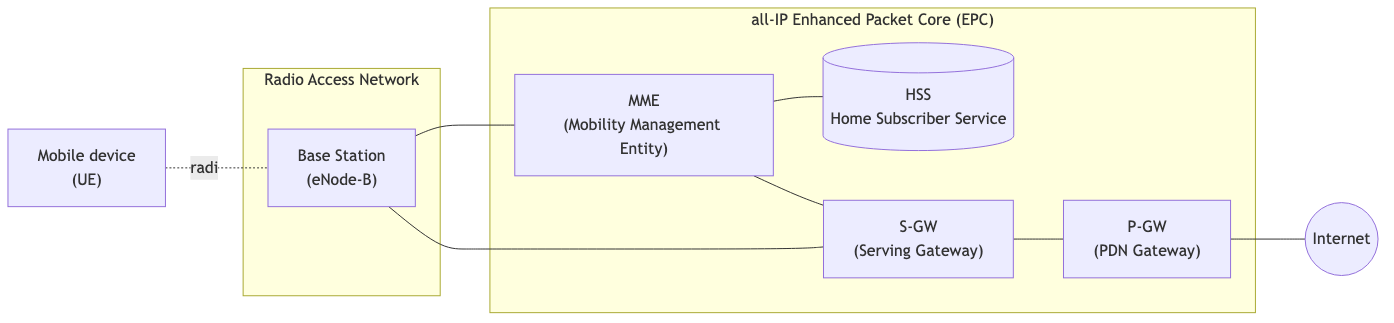
\includegraphics[keepaspectratio]{images/mermaid-lezione-7-lab-mobile-networks-02.png}}
\caption{Topologia logica del 4G LTE. In rosso scuro le interfacce di
controllo (verso MME e HSS), il piano dati attraversa BS → S-GW → P-GW →
Internet.}
\end{figure}

\begin{center}\rule{0.5\linewidth}{0.5pt}\end{center}

\section{Separazione tra Control Plane e Data
Plane}\label{separazione-tra-control-plane-e-data-plane}

Una caratteristica distintiva dell'architettura LTE è la \textbf{netta
separazione fra Piano di Controllo e Piano Dati}. Questa scelta ---
ereditata e amplificata in 5G --- riflette principi di Software Defined
Networking: chi prende le decisioni (MME, HSS) è disaccoppiato da chi
inoltra i pacchetti (S-GW, P-GW).

La Base Station si trova esattamente sull'incrocio dei due piani, e
inoltra \textbf{sia pacchetti di controllo sia pacchetti utente} fra
Mobile Core e UE.

\begin{itemize}
\tightlist
\item
  Nel \textbf{Piano di Controllo}, i pacchetti viaggiano tunnellizzati
  su \textbf{SCTP/IP} (Stream Control Transmission Protocol, RFC 4960).
  SCTP è un'alternativa affidabile a TCP, progettata per trasportare la
  \textbf{segnalazione} delle reti telefoniche; gestisce le procedure di
  registrazione, tracking e autenticazione.
\item
  Nel \textbf{Piano Dati}, i pacchetti utente sono incapsulati nei
  tunnel \textbf{GTP-U} (General Packet Radio Service Tunneling Protocol
  --- User plane), un protocollo 3GPP che opera \textbf{sopra UDP}.
\end{itemize}

\begin{figure}
\centering
\pandocbounded{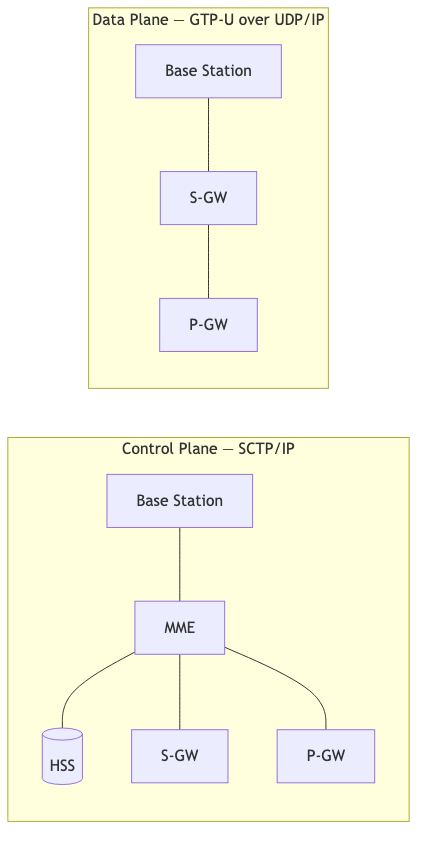
\includegraphics[keepaspectratio]{images/mermaid-lezione-7-lab-mobile-networks-03.png}}
\caption{Separazione Control Plane / Data Plane in LTE. Il control plane
(sopra) trasporta segnalazione su SCTP fra BS, MME, HSS e gateway; il
data plane (sotto) trasporta i pacchetti utente in tunnel GTP-U
attraverso BS → S-GW → P-GW.}
\end{figure}

\begin{callouttip}{Perché la separazione è cruciale}

Disaccoppiare control e data plane permette di scalarli
indipendentemente: si possono aggiungere S-GW per assorbire più traffico
utente senza toccare MME/HSS. Inoltre apre la strada alla
\textbf{virtualizzazione} delle funzioni di controllo (NFV), che in 5G
diventa il principio architetturale dominante.

\end{callouttip}

\begin{center}\rule{0.5\linewidth}{0.5pt}\end{center}

\section{Il tunneling GTP: come la rete supporta la
mobilità}\label{il-tunneling-gtp-come-la-rete-supporta-la-mobilituxe0}

Il datagramma originario emesso dall'UE viene \textbf{incapsulato con
GTP} e spedito dentro un datagramma \textbf{UDP} verso l'S-GW; l'S-GW lo
\emph{re-incapsula} e lo invia al P-GW, che lo ``scarta''
l'incapsulamento e lo immette su Internet. Le sessioni vengono
identificate dal \textbf{TEID} (Tunnel Endpoint Identifier).

\begin{callouttip}{Perché il tunneling GTP abilita la mobilità}

Il tunneling GTP risolve il problema della mobilità IP in modo molto
elegante: incapsulando il datagramma dell'utente dentro un nuovo
pacchetto UDP/GTP, gli \textbf{indirizzi IP visibili a Internet
rimangono fissi} (quelli dell'S-GW e del P-GW). Quando l'utente cambia
cella o si sposta in un'altra area, basta \textbf{aggiornare gli
endpoint del tunnel} --- il dispositivo mantiene il suo indirizzo IP e
le sessioni TCP attive non vengono interrotte.

\end{callouttip}

\begin{figure}
\centering
\pandocbounded{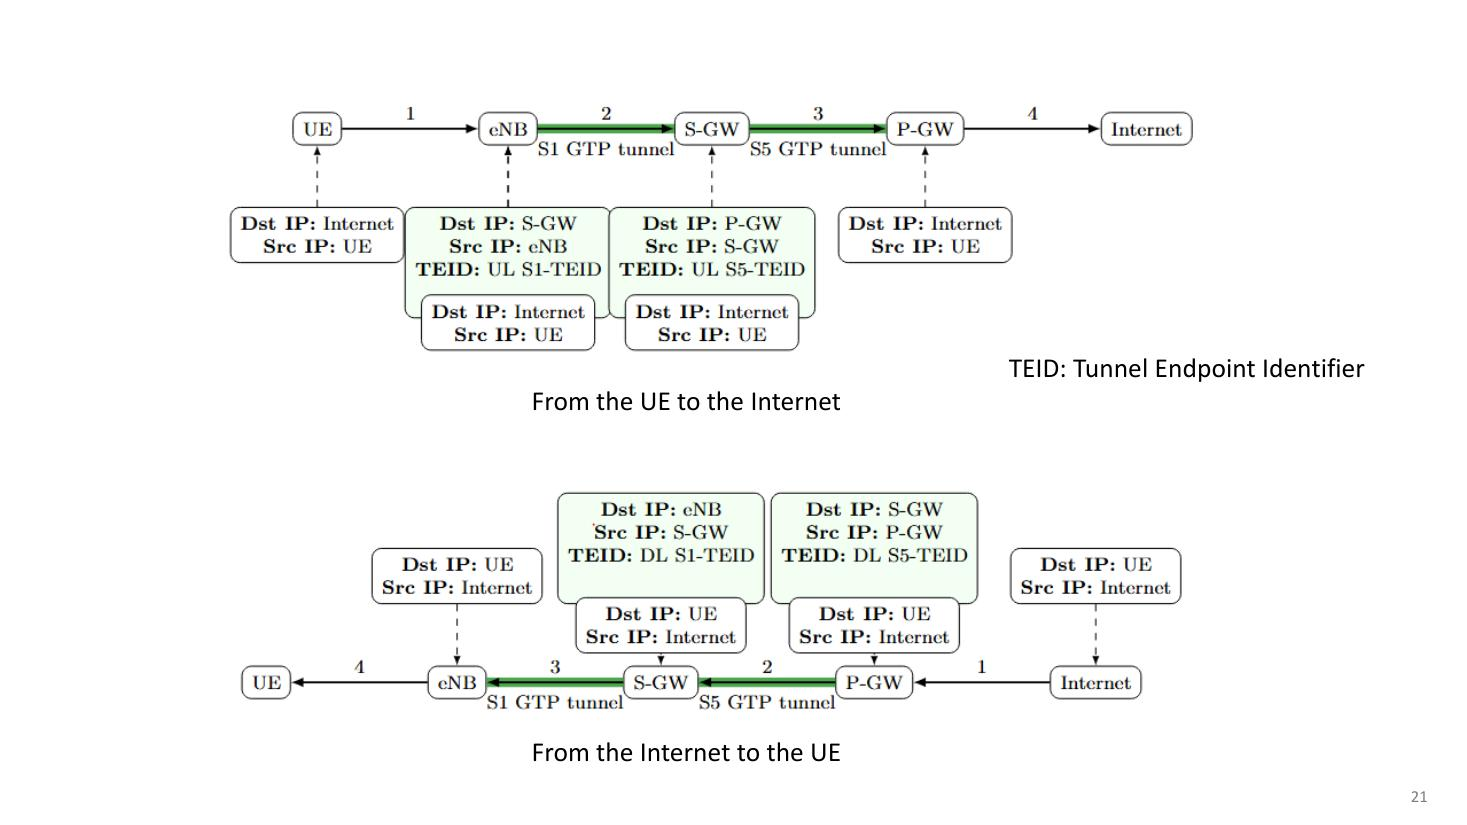
\includegraphics[keepaspectratio]{images/lezione-7-lab-mobile-networks-img-01.jpg}}
\caption{Composizione degli header GTP nel doppio senso del traffico.
\textbf{UE → Internet:} il pacchetto originale
\protect\texttt{Src=UE,\ Dst=Internet} viene incapsulato dall'eNB in un
GTP+UDP+IP con \protect\texttt{Src=eNB,\ Dst=S-GW,\ TEID=UL-S1-TEID}
(tunnel S1); l'S-GW lo ri-incapsula con
\protect\texttt{Src=S-GW,\ Dst=P-GW,\ TEID=UL-S5-TEID} (tunnel S5); il
P-GW rimuove gli incapsulamenti e immette il datagramma originale su
Internet. \textbf{Internet → UE:} il P-GW riceve
\protect\texttt{Src=Internet,\ Dst=UE}, lo incapsula con
\protect\texttt{Src=P-GW,\ Dst=S-GW,\ TEID=DL-S5-TEID}; l'S-GW lo
ri-incapsula verso l'eNB con
\protect\texttt{Src=S-GW,\ Dst=eNB,\ TEID=DL-S1-TEID}; l'eNB consegna il
datagramma all'UE via radio.}
\end{figure}

\begin{center}\rule{0.5\linewidth}{0.5pt}\end{center}

\section{Lo stack del Data Plane LTE}\label{lo-stack-del-data-plane-lte}

A livello radio (cioè fra UE e Base Station), lo stack del piano dati
LTE è composto da quattro livelli specifici, che si frappongono fra il
livello IP ``ordinario'' e l'aria:

\begin{enumerate}
\def\labelenumi{\arabic{enumi}.}
\tightlist
\item
  \textbf{Packet Data Convergence Protocol (PDCP)} --- compressione
  degli header e crittografia.
\item
  \textbf{Radio Link Control (RLC)} --- frammentazione e riassemblaggio
  dei pacchetti IP, trasferimento affidabile a livello di collegamento
  (ACK/NACK).
\item
  \textbf{Medium Access Control (MAC)} --- richiesta e uso degli slot di
  trasmissione radio, rilevazione e correzione degli errori.
\item
  \textbf{Physical Layer} --- modulazione e accesso al canale: FDM e
  TDM, e in particolare \textbf{OFDM} (Orthogonal Frequency Division
  Multiplexing) in downlink, le cui sottoportanti ``ortogonali''
  minimizzano l'interferenza fra canali. Ogni dispositivo attivo riceve
  \textbf{due o più time slot da 0.5 ms} distribuiti su \textbf{12
  frequenze}; lo scheduler non è standardizzato (lo decide l'operatore)
  e rende possibili velocità nell'ordine di \textbf{centinaia di Mbps
  per dispositivo}.
\end{enumerate}

\begin{figure}
\centering
\pandocbounded{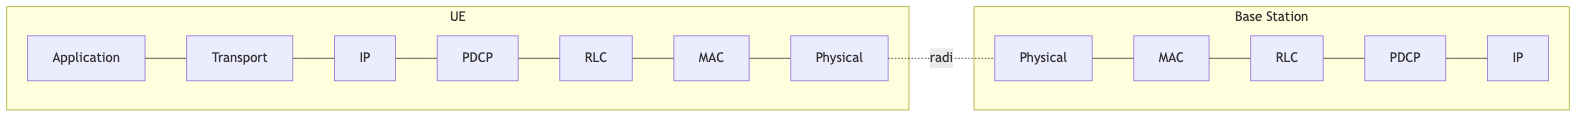
\includegraphics[keepaspectratio]{images/mermaid-lezione-7-lab-mobile-networks-04.png}}
\caption{Stack del data plane LTE sul primo hop UE↔BS. Sopra l'IP
``classico'' si innestano PDCP, RLC, MAC e Physical, che insieme
forniscono compressione, crittografia, riassemblaggio, scheduling e
modulazione OFDM.}
\end{figure}

\begin{center}\rule{0.5\linewidth}{0.5pt}\end{center}

\section{Sleep modes e procedura di
associazione}\label{sleep-modes-e-procedura-di-associazione}

Per preservare la batteria, i dispositivi LTE --- analogamente a Wi-Fi e
Bluetooth --- possono mettere la radio in \textbf{sleep}:

\begin{itemize}
\tightlist
\item
  \textbf{Light sleep} dopo centinaia di millisecondi di inattività; il
  dispositivo si risveglia periodicamente (ogni \textasciitilde100 ms)
  per controllare se ci sono trasmissioni in arrivo.
\item
  \textbf{Deep sleep} dopo 5--10 secondi di inattività. In deep sleep il
  dispositivo potrebbe \textbf{cambiare cella}, quindi al risveglio deve
  \textbf{ristabilire l'associazione} per ricevere i messaggi di
  \textbf{paging} broadcastati dall'MME quando qualcuno cerca di
  contattarlo (chiamata, SMS, dato in arrivo).
\end{itemize}

\begin{calloutnote}{Cos’è il paging}

Quando qualcuno tenta di chiamare o inviare un messaggio a un
dispositivo, la rete deve prima localizzarlo. L'MME \textbf{broadcasta}
messaggi di paging nell'area in cui il dispositivo è probabilmente
presente (la ``tracking area''). Il dispositivo, ricevuto il paging,
esce dal deep sleep e si ri-associa per ricevere il dato.

\end{calloutnote}

La \textbf{procedura di associazione} a una rete avviene in più passi:

\begin{enumerate}
\def\labelenumi{\arabic{enumi}.}
\tightlist
\item
  La BS broadcasta ogni 5 ms un \textbf{primary synch signal} su tutte
  le frequenze. Più carrier diversi possono star broadcastando in
  parallelo.
\item
  Il dispositivo individua il primary synch signal e poi il
  \textbf{secondary synch signal} sulla stessa frequenza.
\item
  Legge le informazioni broadcastate dalla BS: larghezza di banda,
  configurazioni, info sul carrier cellulare.
\item
  Il dispositivo \textbf{seleziona la BS} a cui associarsi (preferendo
  tipicamente il proprio carrier home).
\item
  Seguono altri passi per \textbf{autenticarsi}, stabilire stato e
  configurare il piano dati.
\end{enumerate}

\begin{center}\rule{0.5\linewidth}{0.5pt}\end{center}

\section{La rivoluzione del 5G: prestazioni e use
case}\label{la-rivoluzione-del-5g-prestazioni-e-use-case}

Mentre il 4G mirava a circa 10 Mbps e 10 ms di latenza, il 5G alza
drasticamente l'asticella (proiezioni GAO e ITU):

\begin{itemize}
\tightlist
\item
  \textbf{10× il bitrate di picco} --- 100 Mbps di ``User experienced
  data rate'' sostenuti, con picchi potenziali \(> 10\) Gbps;
\item
  \textbf{10× più bassa la latenza} --- fino a \textbf{1 ms};
\item
  \textbf{100× più capacità di traffico}, e una \textbf{densità di
  connessione} che supporta \textbf{1 milione di dispositivi per km²}.
\end{itemize}

La nuova radio \textbf{5G NR (New Radio)} \textbf{non è
retrocompatibile} con il 4G. Opera su due bande principali:

\begin{itemize}
\tightlist
\item
  \textbf{FR1} --- 450 MHz -- 6 GHz (microonde ``tradizionali'', buona
  copertura);
\item
  \textbf{FR2} --- 24 GHz -- 52 GHz (\textbf{onde millimetriche},
  mmWave).
\end{itemize}

Le frequenze millimetriche permettono velocità immense ma su distanze
brevi: questo richiede antenne direzionali (\textbf{MIMO},
Multiple-Input Multiple-Output) e un'installazione \textbf{densissima}
di nuove stazioni base, le \textbf{pico-cells}, con raggio di soli
10--100 m.

\subsection{I tre macro-scenari d'uso}\label{i-tre-macro-scenari-duso}

\begin{callouttip}{eMBB — Enhanced Mobile Broadband}

Larghezza di banda incrementata per applicazioni multimediali pesanti:
realtà aumentata e virtuale, video streaming 4K/360°. Si punta a
\emph{data rate} multi-Gbps di picco, 100+ Mbps sostenuti, e capacità
aggregata di 10 Tbps per km².

\end{callouttip}

\begin{callouttip}{URLLC — Ultra Reliable Low-Latency Communications}

Applicazioni mission-critical altamente sensibili alla latenza:
automazione di fabbrica, \textbf{guida autonoma}. Richiede affidabilità
``five nines'' (99.999\%), latenza \textbf{1 ms} e supporto della
mobilità ad alta velocità (fino a 100 km/h).

\end{callouttip}

\begin{callouttip}{mMTC — Massive Machine Type Communications}

Accesso \emph{narrowband} per pervasività sensoriale: metering,
monitoring, IoT diffuso. Dispositivi \textbf{ultra-low-power} (10+ anni
di batteria), ultra-low-complexity (decine di bit/s), ultra-high density
(1M nodi/km²).

\end{callouttip}

\begin{center}\rule{0.5\linewidth}{0.5pt}\end{center}

\section{La 5G Core e la Service Based
Architecture}\label{la-5g-core-e-la-service-based-architecture}

A livello architetturale il 5G Core (NG-Core) è profondamente
riprogettato per integrarsi con Internet e con i servizi cloud.
L'approccio è \textbf{cloud-native}: la rete è organizzata come un set
di \textbf{Network Functions (NF)} indipendenti, riutilizzabili e
implementabili come macchine virtuali o container su hardware generico
(\textbf{Network Function Virtualization, NFV}). Le NF possono essere
lanciate e rilasciate dinamicamente in base al carico.

Ogni Network Function espone i propri servizi tramite una
\textbf{Service-Based Interface (SBI)}, un'interfaccia REST ben definita
su \textbf{HTTP/2}. È un cambio paradigmatico: le funzioni di rete
diventano \textbf{microservizi} che si chiamano tra loro come fossero
API web.

Alcuni concetti rimangono comunque ereditati dal 4G --- primo fra tutti
l'incapsulamento dei pacchetti via \textbf{GTP-U} sul piano utente. La
separazione fra control e user plane viene portata all'estremo, e i
server vengono distribuiti \textbf{fino all'edge} della rete per ridurre
la latenza.

\subsection{Mapping 4G → 5G delle
funzioni}\label{mapping-4g-5g-delle-funzioni}

{\def\LTcaptype{none} % do not increment counter
\begin{longtable}[]{@{}
  >{\raggedright\arraybackslash}p{(\linewidth - 4\tabcolsep) * \real{0.3333}}
  >{\raggedright\arraybackslash}p{(\linewidth - 4\tabcolsep) * \real{0.3333}}
  >{\raggedright\arraybackslash}p{(\linewidth - 4\tabcolsep) * \real{0.3333}}@{}}
\toprule\noalign{}
\begin{minipage}[b]{\linewidth}\raggedright
\textbf{Componente 4G}
\end{minipage} & \begin{minipage}[b]{\linewidth}\raggedright
\textbf{Corrispettivo 5G}
\end{minipage} & \begin{minipage}[b]{\linewidth}\raggedright
\textbf{Funzione}
\end{minipage} \\
\midrule\noalign{}
\endhead
\bottomrule\noalign{}
\endlastfoot
\textbf{eNB} & \textbf{gNB} & Radio 5G modulare e cloud-native,
splittata in \emph{Distributed Unit} e \emph{Central Unit} per
deployment flessibile \\
\textbf{S-GW + P-GW} & \textbf{UPF} (User Plane Function) & Inoltra il
traffico fra RAN e Internet; gestisce packet inspection, QoS e
reporting; può essere distribuita per Multi-Access Edge Computing
(MEC) \\
\textbf{MME} & \textbf{AMF + SMF} & \textbf{AMF} (Access and Mobility
Management Function): autenticazione, gestione connessione, mobilità,
reachability. \textbf{SMF} (Session Management Function): gestione
sessioni dati, allocazione IP, controllo QoS e routing user-plane \\
\textbf{HSS} & \textbf{AUSF + UDM} & \textbf{AUSF} (Authentication
Server Function): procedure di autenticazione. \textbf{UDM} (Unified
Data Management): identità degli utenti, credenziali, dati di
abbonamento \\
\textbf{PCRF} & \textbf{PCF} & Policy Control Function --- definisce le
regole di policy che le altre NF di controllo applicano \\
\end{longtable}
}

Il 5G introduce inoltre \textbf{Network Function di supporto} (helper)
totalmente nuove, che rendono i servizi \emph{stateless} e quindi
facilmente scalabili:

\begin{itemize}
\tightlist
\item
  \textbf{SDSF} (Structured Data Storage Network Function) e
  \textbf{UDSF} (Unstructured Data Storage Network Function) --- servizi
  di archiviazione dati centralizzati: estraendo lo stato dalle altre
  NF, queste possono restare stateless.
\item
  \textbf{NEF} (Network Exposure Function) --- espone in modo
  controllato e sicuro le capacità della rete a servizi di terze parti.
\item
  \textbf{NRF} (NF Repository Function) --- registry per la
  \emph{service discovery} delle NF disponibili.
\item
  \textbf{NSSF} (Network Slicing Selector Function) --- seleziona la
  \textbf{Network Slice} appropriata per ogni UE, permettendo di
  partizionare logicamente la rete e differenziare il servizio fra
  utenti/tenant.
\end{itemize}

\begin{callouttip}{La logica cloud-native}

Avere storage separato (SDSF/UDSF) e un registry di servizi (NRF) non è
un dettaglio tecnico: è esattamente lo stesso \emph{pattern} di
un'architettura a microservizi cloud (12-factor, Kubernetes-style).
Permette di \textbf{scalare orizzontalmente} una NF aggiungendo istanze,
di \textbf{sostituire un'istanza} in caso di guasto senza perdere stato,
e di esporre a terzi (NEF) capacità di rete come API consumabili.

\end{callouttip}

\subsection{UPF e Multi-Access Edge
Computing}\label{upf-e-multi-access-edge-computing}

Particolarmente importante è il ruolo dell'\textbf{UPF}: corrispondente
unificato di S-GW + P-GW, può essere replicato e distribuito in
molteplici punti della rete, anche \textbf{all'edge} vicino agli utenti.
Questa flessibilità abilita il \textbf{Multi-Access Edge Computing
(MEC)}, in cui le \textbf{VNF} (Virtual Network Functions) e i workload
applicativi possono essere co-locati con l'UPF stesso, riducendo
drasticamente la latenza per scenari URLLC.

\begin{figure}
\centering
\pandocbounded{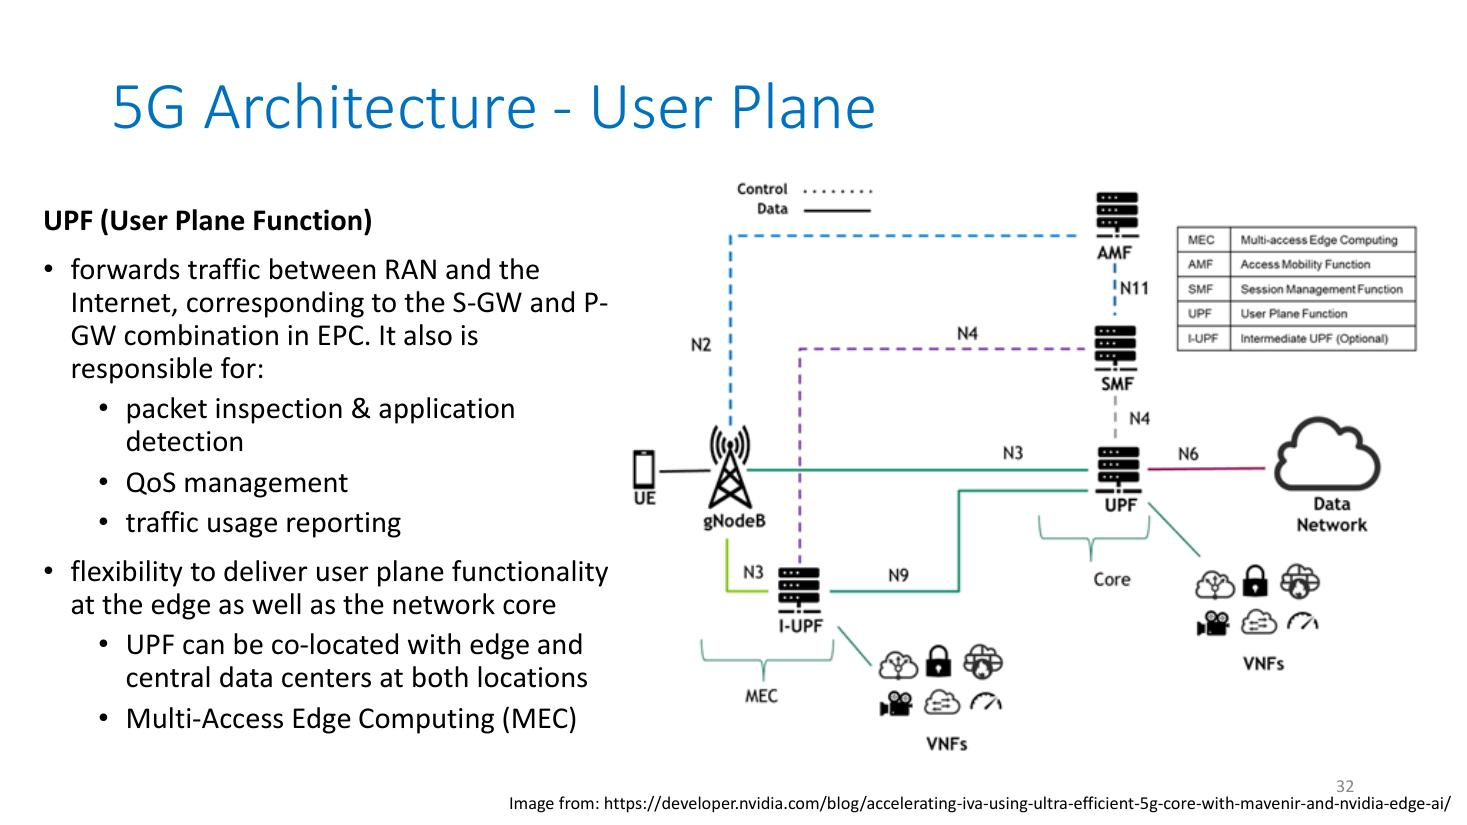
\includegraphics[keepaspectratio]{images/lezione-7-lab-mobile-networks-img-02.jpg}}
\caption{Architettura 5G User Plane (immagine NVIDIA/Mavenir). Il
\textbf{gNodeB} dialoga con un'\textbf{I-UPF} (Intermediate UPF)
all'edge tramite l'interfaccia N3, raggiungendo il core via N9 fino
all'\textbf{UPF} centrale che si interfaccia col Data Network (N6). Il
control plane (linee tratteggiate) --- \textbf{AMF}, \textbf{SMF} ---
comunica con i nodi user-plane via N2, N4, N11. Le \textbf{VNF} all'edge
realizzano il MEC.}
\end{figure}

\begin{center}\rule{0.5\linewidth}{0.5pt}\end{center}

\section{Opzioni di deployment: Standalone vs
Non-Standalone}\label{opzioni-di-deployment-standalone-vs-non-standalone}

Il passaggio da 4G a 5G non è atomico: gli operatori possono scegliere
fra diverse strategie di deployment.

{\def\LTcaptype{none} % do not increment counter
\begin{longtable}[]{@{}
  >{\raggedright\arraybackslash}p{(\linewidth - 6\tabcolsep) * \real{0.2500}}
  >{\raggedright\arraybackslash}p{(\linewidth - 6\tabcolsep) * \real{0.2500}}
  >{\raggedright\arraybackslash}p{(\linewidth - 6\tabcolsep) * \real{0.2500}}
  >{\raggedright\arraybackslash}p{(\linewidth - 6\tabcolsep) * \real{0.2500}}@{}}
\toprule\noalign{}
\begin{minipage}[b]{\linewidth}\raggedright
Modalità
\end{minipage} & \begin{minipage}[b]{\linewidth}\raggedright
RAN
\end{minipage} & \begin{minipage}[b]{\linewidth}\raggedright
Core
\end{minipage} & \begin{minipage}[b]{\linewidth}\raggedright
Note
\end{minipage} \\
\midrule\noalign{}
\endhead
\bottomrule\noalign{}
\endlastfoot
\textbf{Standalone 4G} & 4G & EPC & Rete 4G ``pura'' \\
\textbf{Non-Standalone (NSA)} & 4G + 5G & EPC (4G) & Le BS 5G affiancano
quelle 4G per dare un \emph{boost} di capacità; il \textbf{piano di
controllo passa attraverso le BS 4G} verso il Core 4G, mentre le BS 5G
veicolano \textbf{solo traffico utente} \\
\textbf{NSA su NG-Core} & 4G + 5G & NG-Core (5G) & Variante con BS 4G+5G
ma core già migrato al 5G \\
\textbf{Standalone 5G} & 5G & NG-Core & 5G ``puro'': sia controllo che
dati gestiti dal NG-Core \\
\end{longtable}
}

\begin{calloutwarning}{Adozione del 5G SA molto disomogenea}

Secondo i dati Ookla 2025, l'adozione del 5G Standalone varia
enormemente nel mondo: \textbf{80\% in Cina}, \textbf{52\% in India},
\textbf{24\% negli Stati Uniti}, ma \textbf{solo 2\% in Europa}.
L'Europa è in forte ritardo sull'adozione del 5G ``puro'' e la
maggioranza delle reti è ancora in modalità NSA.

\end{calloutwarning}

\begin{center}\rule{0.5\linewidth}{0.5pt}\end{center}

\section{La rete cellulare come ``rete di reti
IP''}\label{la-rete-cellulare-come-rete-di-reti-ip}

Le reti cellulari globali formano oggi una complessa ``rete di reti IP''
interconnesse tramite punti di interscambio chiamati \textbf{IPX} (IP
eXchange). Pur condividendo molte tecnologie con Internet (HTTP, DNS,
TCP/UDP, NAT, separazione control/data, SDN, Ethernet, tunneling),
conservano alcune \textbf{specificità}:

{\def\LTcaptype{none} % do not increment counter
\begin{longtable}[]{@{}
  >{\raggedright\arraybackslash}p{(\linewidth - 4\tabcolsep) * \real{0.3333}}
  >{\raggedright\arraybackslash}p{(\linewidth - 4\tabcolsep) * \real{0.3333}}
  >{\raggedright\arraybackslash}p{(\linewidth - 4\tabcolsep) * \real{0.3333}}@{}}
\toprule\noalign{}
\begin{minipage}[b]{\linewidth}\raggedright
\end{minipage} & \begin{minipage}[b]{\linewidth}\raggedright
\textbf{Internet cablata}
\end{minipage} & \begin{minipage}[b]{\linewidth}\raggedright
\textbf{Reti cellulari 4G/5G}
\end{minipage} \\
\midrule\noalign{}
\endhead
\bottomrule\noalign{}
\endlastfoot
Mobilità & non nativa & servizio di \textbf{prima classe} \\
Identità utente & varia (IP, account, ecc.) & fortemente legata alla
\textbf{SIM card} \\
Modello di business & best-effort, peering & \textbf{abbonamento} a un
carrier specifico \\
Home vs visited & non significativo & distinzione fondamentale, regola
il \textbf{roaming} \\
Link di accesso & tipicamente cablato & \textbf{radio}, con tutti i suoi
vincoli \\
\end{longtable}
}

Il \textbf{roaming} --- l'uso della rete da parte di un abbonato fuori
dalla propria home network --- è regolato dal \textbf{rapporto di
fiducia commerciale} fra rete home e rete visitata: è la home network
(che possiede l'HSS con i dati dell'abbonato) a ``garantire'' per
l'utente, mentre la rete visitata fornisce l'accesso e poi regola
economicamente i costi con la home.

\begin{figure}
\centering
\pandocbounded{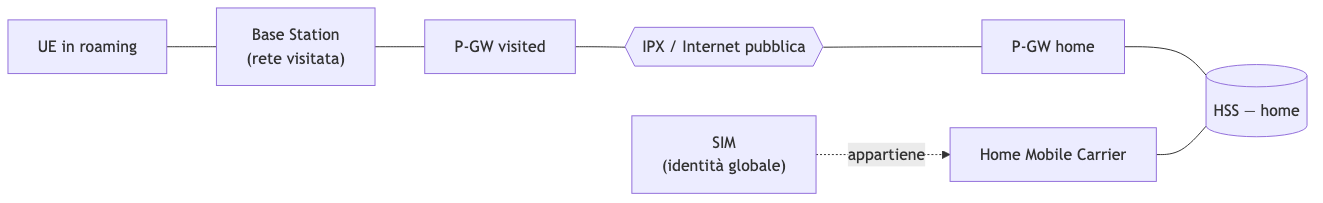
\includegraphics[keepaspectratio]{images/mermaid-lezione-7-lab-mobile-networks-05.png}}
\caption{Roaming in una rete globale di carrier interconnessi via IPX.
La SIM lega l'utente alla home network; quando è in roaming, la rete
visitata si appoggia all'HSS della home per autenticare e autorizzare
l'utente.}
\end{figure}

\begin{center}\rule{0.5\linewidth}{0.5pt}\end{center}

\section{Sicurezza e autenticazione in 4G LTE: il protocollo
AKA}\label{sicurezza-e-autenticazione-in-4g-lte-il-protocollo-aka}

Quando un dispositivo arriva in una rete (anche visitata), deve compiere
\textbf{due operazioni distinte}:

\begin{enumerate}
\def\labelenumi{\arabic{enumi}.}
\tightlist
\item
  \textbf{Associarsi alla BS} --- stabilire la comunicazione sul canale
  radio 4G;
\item
  \textbf{Autenticarsi alla rete} --- e contemporaneamente
  \textbf{autenticare la rete} (mutua autenticazione).
\end{enumerate}

A differenza del Wi-Fi, qui la \textbf{SIM card fornisce l'identità
globale} dell'utente, e i servizi disponibili nella rete visitata
dipendono da una \textbf{subscription pagata} nella home network.
\textbf{MME nella rete visitata} e \textbf{HSS nella rete home} giocano
insieme il ruolo dell'Authentication Server di un access point Wi-Fi: il
vero ``ultimate authenticator'' è l'HSS, ma le decisioni passano
dall'MME visitato.

\begin{calloutdefinition}{AKA — Authentication and Key Agreement}

Protocollo di autenticazione \textbf{challenge-and-response} definito da
3GPP, basato su \textbf{chiave simmetrica} condivisa fra abbonato e home
network. Garantisce \textbf{autenticazione} delle entità,
\textbf{integrità} e \textbf{confidenzialità} dei messaggi. Dopo la
mutua autenticazione, vengono derivate chiavi crittografiche per
proteggere sia la signaling sia i dati del piano utente.

\end{calloutdefinition}

Vediamo passo-passo come funziona, con particolare attenzione al
\emph{perché} la mutua autenticazione regge.

\begin{figure}
\centering
\pandocbounded{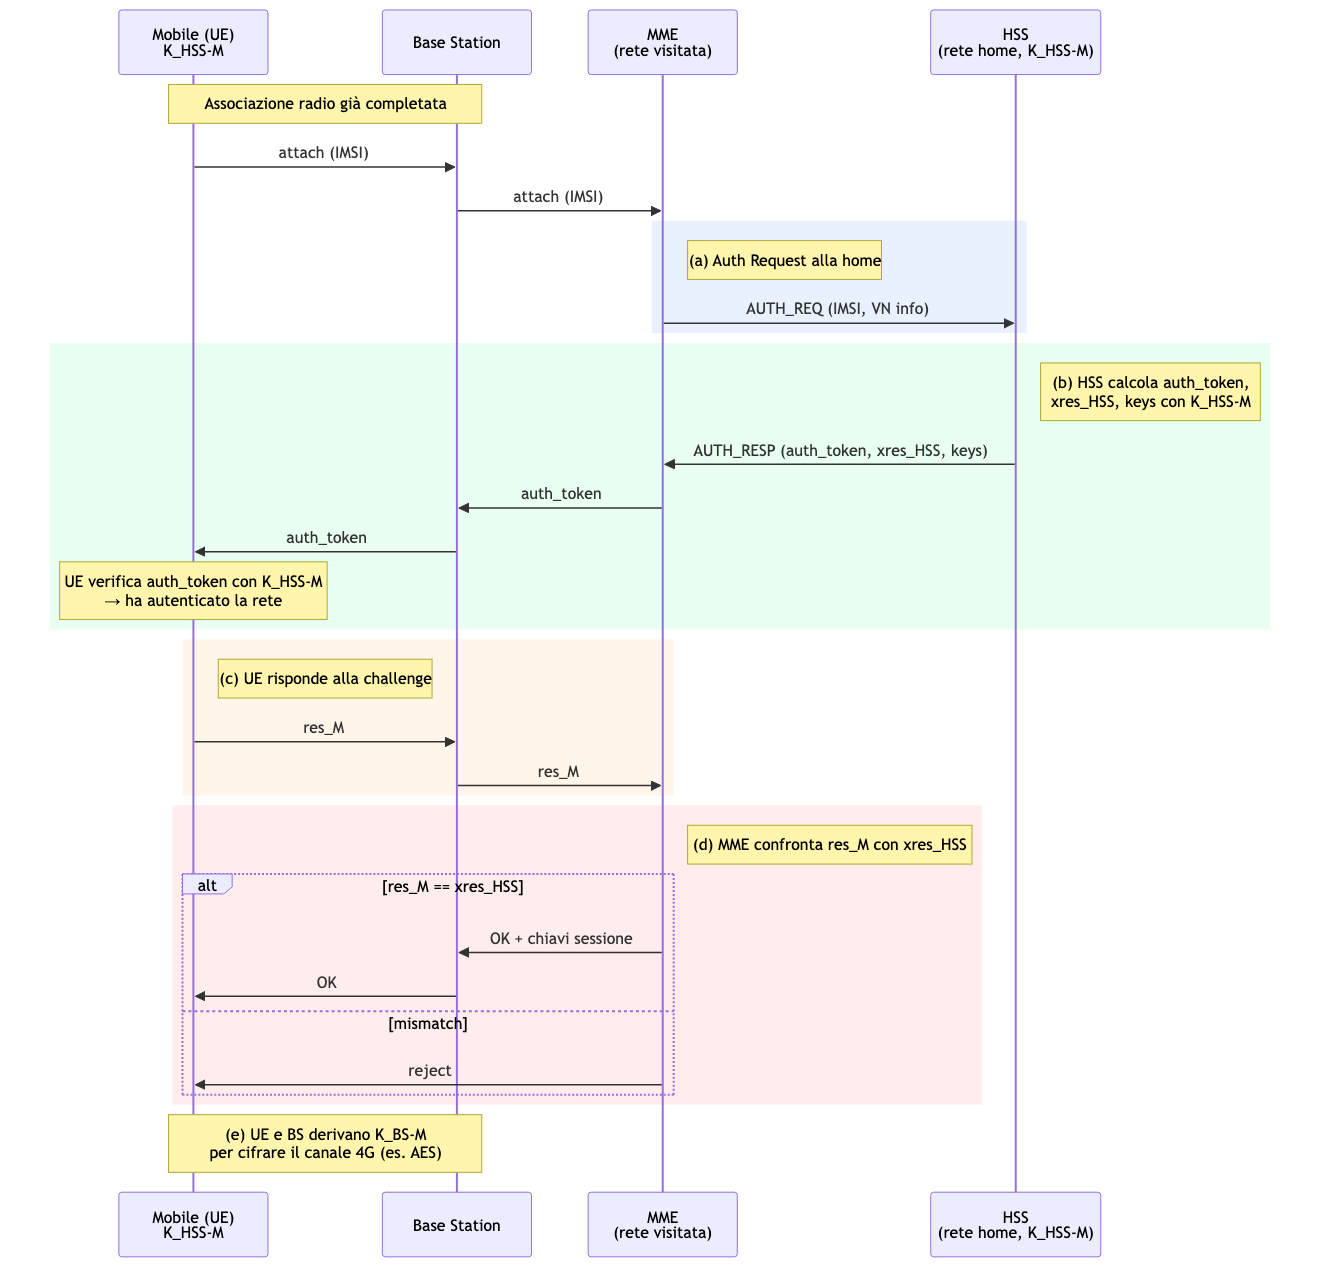
\includegraphics[keepaspectratio]{images/mermaid-lezione-7-lab-mobile-networks-06.png}}
\caption{Sequence diagram del protocollo AKA in 4G LTE. Le cinque fasi
(a)\ldots(e) corrispondono ai passi numerati delle slide.}
\end{figure}

\subsection{I cinque passi di AKA, in
dettaglio}\label{i-cinque-passi-di-aka-in-dettaglio}

\textbf{(a) Attach + AUTH\_REQ.} L'UE invia un messaggio di
\emph{attach} contenente il proprio \textbf{IMSI}. La BS lo inoltra
all'MME della rete visitata, che a sua volta gira IMSI + informazioni
della rete visitata (\texttt{VN\ info}) all'\textbf{HSS} nella home
network del dispositivo. L'IMSI identifica esplicitamente la home
network, quindi l'MME sa a chi rivolgersi.

\textbf{(b) HSS genera la challenge.} L'HSS, usando la \textbf{chiave
segreta pre-condivisa} \(K_{HSS\text{-}M}\) (memorizzata in modo sicuro
sulla SIM dal lato UE, e nel database dell'HSS dal lato rete), calcola:

\begin{itemize}
\tightlist
\item
  un \textbf{auth\_token} che contiene informazioni cifrate con
  \(K_{HSS\text{-}M}\);
\item
  la \textbf{risposta attesa} \(\text{xres}_{HSS}\) (la ``verifica''
  della challenge);
\item
  le \textbf{chiavi di sessione}.
\end{itemize}

\textless\textless\textless\textless\textless\textless\textless{} HEAD
Manda \texttt{(auth\_token,\ xres\_HSS,\ keys)} all'MME, che inoltra
solo l'\texttt{auth\_token} all'UE attraverso la BS. L'UE, possedendo
lui pure \(K_{HSS\text{-}M}\), \textbf{decifra e verifica
matematicamente} l'auth-token: se torna, significa che l'altra parte
conosce davvero la chiave segreta --- quindi è la vera home network.
\textbf{A questo punto l'UE ha autenticato la rete.} Nel frattempo l'MME
tiene da parte \(\text{xres}_{HSS}\) per il passo (d). ======= Manda
\texttt{(auth\_token,\ xres\_HSS,\ keys)} all'MME, che inoltra solo
l'\texttt{auth\_token} all'UE attraverso la BS. L'UE, possedendo lui
pure \(K_{HSS\text{-}M}\), \textbf{decifra e verifica matematicamente}
l'auth\_token: se torna, significa che l'altra parte conosce davvero la
chiave segreta --- quindi è la vera home network. \textbf{A questo punto
l'UE ha autenticato la rete.} Nel frattempo l'MME tiene da parte
\(\text{xres}_{HSS}\) per il passo (d).
\textgreater\textgreater\textgreater\textgreater\textgreater\textgreater\textgreater{}
origin/main

\textbf{(c) UE risponde.} L'UE esegue \textbf{lo stesso calcolo
crittografico} che ha fatto l'HSS, usando la sua copia di
\(K_{HSS\text{-}M}\), ottenendo \(\text{res}_{M}\). Lo invia all'MME via
BS.

\textbf{(d) MME valida.} L'MME confronta \(\text{res}_{M}\) (calcolato
dall'UE) con \(\text{xres}_{HSS}\) (calcolato dall'HSS). Se coincidono,
\textbf{la rete ha autenticato l'UE} --- perché solo chi possiede
\(K_{HSS\text{-}M}\) poteva ottenere quel valore. L'MME informa la BS
dell'avvenuta autenticazione e genera le chiavi di sessione per la BS.

\textbf{(e) Derivazione delle chiavi radio.} UE e BS, a partire dal
materiale crittografico scambiato, derivano la chiave
\(K_{BS\text{-}M}\) con cui cifrano dati e frame di controllo sul canale
wireless 4G --- tipicamente con \textbf{AES}.

\begin{calloutquestion}{Perché il confronto \\text\{res\}\_M = \\text\{xres\}\_\{HSS\} basta a dimostrare l’identità dell’UE?}

Perché la funzione che calcola la response è \textbf{deterministica e
dipende dalla chiave segreta} \(K_{HSS\text{-}M}\). Solo due entità la
conoscono: la SIM dell'utente e l'HSS. Se il valore calcolato dall'UE
coincide con quello calcolato dall'HSS, è praticamente impossibile
(sotto le ipotesi crittografiche standard) che l'UE non possieda la
chiave --- quindi è autentico. La presenza di un \emph{nonce}
freschissimo nella challenge previene attacchi di replay.

\end{calloutquestion}

\begin{center}\rule{0.5\linewidth}{0.5pt}\end{center}

\section{Sicurezza in 5G: cosa cambia rispetto al
4G}\label{sicurezza-in-5g-cosa-cambia-rispetto-al-4g}

Il 5G mantiene la struttura concettuale di AKA ma ne irrobustisce due
aspetti chiave, entrambi rivolti a chiudere falle di privacy/fiducia
presenti in 4G.

{\def\LTcaptype{none} % do not increment counter
\begin{longtable}[]{@{}
  >{\raggedright\arraybackslash}p{(\linewidth - 4\tabcolsep) * \real{0.3333}}
  >{\raggedright\arraybackslash}p{(\linewidth - 4\tabcolsep) * \real{0.3333}}
  >{\raggedright\arraybackslash}p{(\linewidth - 4\tabcolsep) * \real{0.3333}}@{}}
\toprule\noalign{}
\begin{minipage}[b]{\linewidth}\raggedright
Aspetto
\end{minipage} & \begin{minipage}[b]{\linewidth}\raggedright
4G
\end{minipage} & \begin{minipage}[b]{\linewidth}\raggedright
5G
\end{minipage} \\
\midrule\noalign{}
\endhead
\bottomrule\noalign{}
\endlastfoot
\textbf{Decisione di autenticazione} & Presa dall'\textbf{MME nella rete
visitata} & Presa dalla \textbf{rete home}; l'AMF visitato fa da
``middleman'' (può comunque rifiutare la connessione) \\
\textbf{Trasmissione dell'IMSI} & Inviato \textbf{in chiaro} alla BS al
momento dell'attach & Cifrato con \textbf{crittografia a chiave
pubblica} prima di essere trasmesso \\
\end{longtable}
}

\begin{calloutwarning}{L’IMSI in chiaro era un problema serio}

In 4G l'IMSI viaggiava in cleartext sulla prima porzione del protocollo
di attach: questo permetteva attacchi noti come \textbf{IMSI catcher}
(``Stingray''), apparati che si fingono BS legittime per intercettare
gli IMSI dei dispositivi vicini e tracciare gli utenti. Il 5G chiude
questa falla cifrando l'identificativo con una \textbf{chiave pubblica
della home network}: solo l'home network può decifrarlo, la rete
visitata e gli intercettatori vedono solo un identificativo
``schermato'' (SUCI --- SUbscription Concealed Identifier).

\end{calloutwarning}

\begin{calloutnote}{Centralizzare la decisione nella home}

Spostare la decisione finale di autenticazione dalla rete visitata alla
rete home riduce la superficie di attacco: anche se un MME visitato
viene compromesso, da solo non può ``creare'' abbonati validi. La rete
visitata mantiene comunque potere di veto sulla connessione (può
rifiutare per policy locali), ma non può approvarla autonomamente.

\end{calloutnote}

\begin{center}\rule{0.5\linewidth}{0.5pt}\end{center}

\begin{calloutnote}{Sintesi}

L'evoluzione dalle reti cellulari analogiche al 5G è una trasformazione
architetturale, non solo un aumento di velocità. Il cuore della
trasformazione è il passaggio a un \textbf{All-IP core} (introdotto in
4G con l'EPC) e poi a una \textbf{Service Based Architecture
cloud-native} (in 5G con l'NG-Core), con netta separazione di control
plane e data plane e con le funzioni di rete organizzate come
\textbf{microservizi} indipendenti. Il \textbf{tunneling GTP} è il
pilastro che abilita la mobilità trasparente: gli IP del traffico
restano fissi, cambiano solo gli endpoint dei tunnel quando l'utente si
sposta. Il protocollo \textbf{AKA} garantisce mutua autenticazione
UE↔rete sfruttando una chiave simmetrica condivisa fra SIM e home HSS;
il 5G rafforza la sicurezza spostando la decisione finale alla home
network e cifrando l'IMSI con crittografia a chiave pubblica per
prevenire attacchi di tracciamento. Sul fronte radio, \textbf{5G NR}
combina sub-6 GHz e onde millimetriche con MIMO e densità di celle
elevate, abilitando i tre macro-scenari \textbf{eMBB}, \textbf{URLLC} e
\textbf{mMTC}.

\end{calloutnote}

\newpage

\chapter{Mobile Networks --- Mobilità nelle Reti
Cellulari}\label{mobile-networks-mobilituxe0-nelle-reti-cellulari}

La mobilità nelle reti di telecomunicazione moderne si estende lungo un
ampio spettro: dall'assenza totale di spostamento fino a scenari in cui
un dispositivo attraversa reti di operatori diversi mantenendo attive le
proprie sessioni. Questo capitolo analizza le architetture che rendono
possibile tale mobilità --- in particolare nelle reti 4G/5G ---
esaminando i meccanismi di registrazione, i due approcci di routing
(indiretto e diretto) e le procedure di \emph{handover} tra stazioni
base.

\begin{center}\rule{0.5\linewidth}{0.5pt}\end{center}

\section{Lo Spettro della Mobilità e la Home
Network}\label{lo-spettro-della-mobilituxe0-e-la-home-network}

Dal punto di vista infrastrutturale, la mobilità non è una proprietà
binaria ma uno spettro continuo. A un estremo si trovano dispositivi
completamente statici; procedendo si incontrano dispositivi che cambiano
rete solo tra una sessione e l'altra, o che si muovono tra Access Point
dello stesso operatore. L'estremo di maggiore interesse è l'\textbf{alta
mobilità}: un dispositivo che cambia rete mantenendo attive le
connessioni in corso.

Per gestire questo livello di mobilità è indispensabile il concetto di
\textbf{home network}: una fonte autorevole e centralizzata che registra
la posizione attuale del dispositivo e dalla quale le altre entità di
rete possono ottenerla. Senza di essa non esiste modo affidabile di
recapitare traffico a un nodo in movimento.

\subsection{Reti 4G/5G vs ISP/WiFi}\label{reti-4g5g-vs-ispwifi}

Nelle reti cellulari \textbf{4G/5G} la home network corrisponde alla
rete dell'operatore con cui l'utente ha sottoscritto il contratto (es.
Verizon, Orange). Il database centrale che memorizza identità e servizi
abilitati è l'\textbf{Home Subscriber Server (HSS)}. L'identità globale
del dispositivo --- inclusa la sua rete di appartenenza --- è codificata
nella \textbf{SIM card}.

\begin{figure}
\centering
\pandocbounded{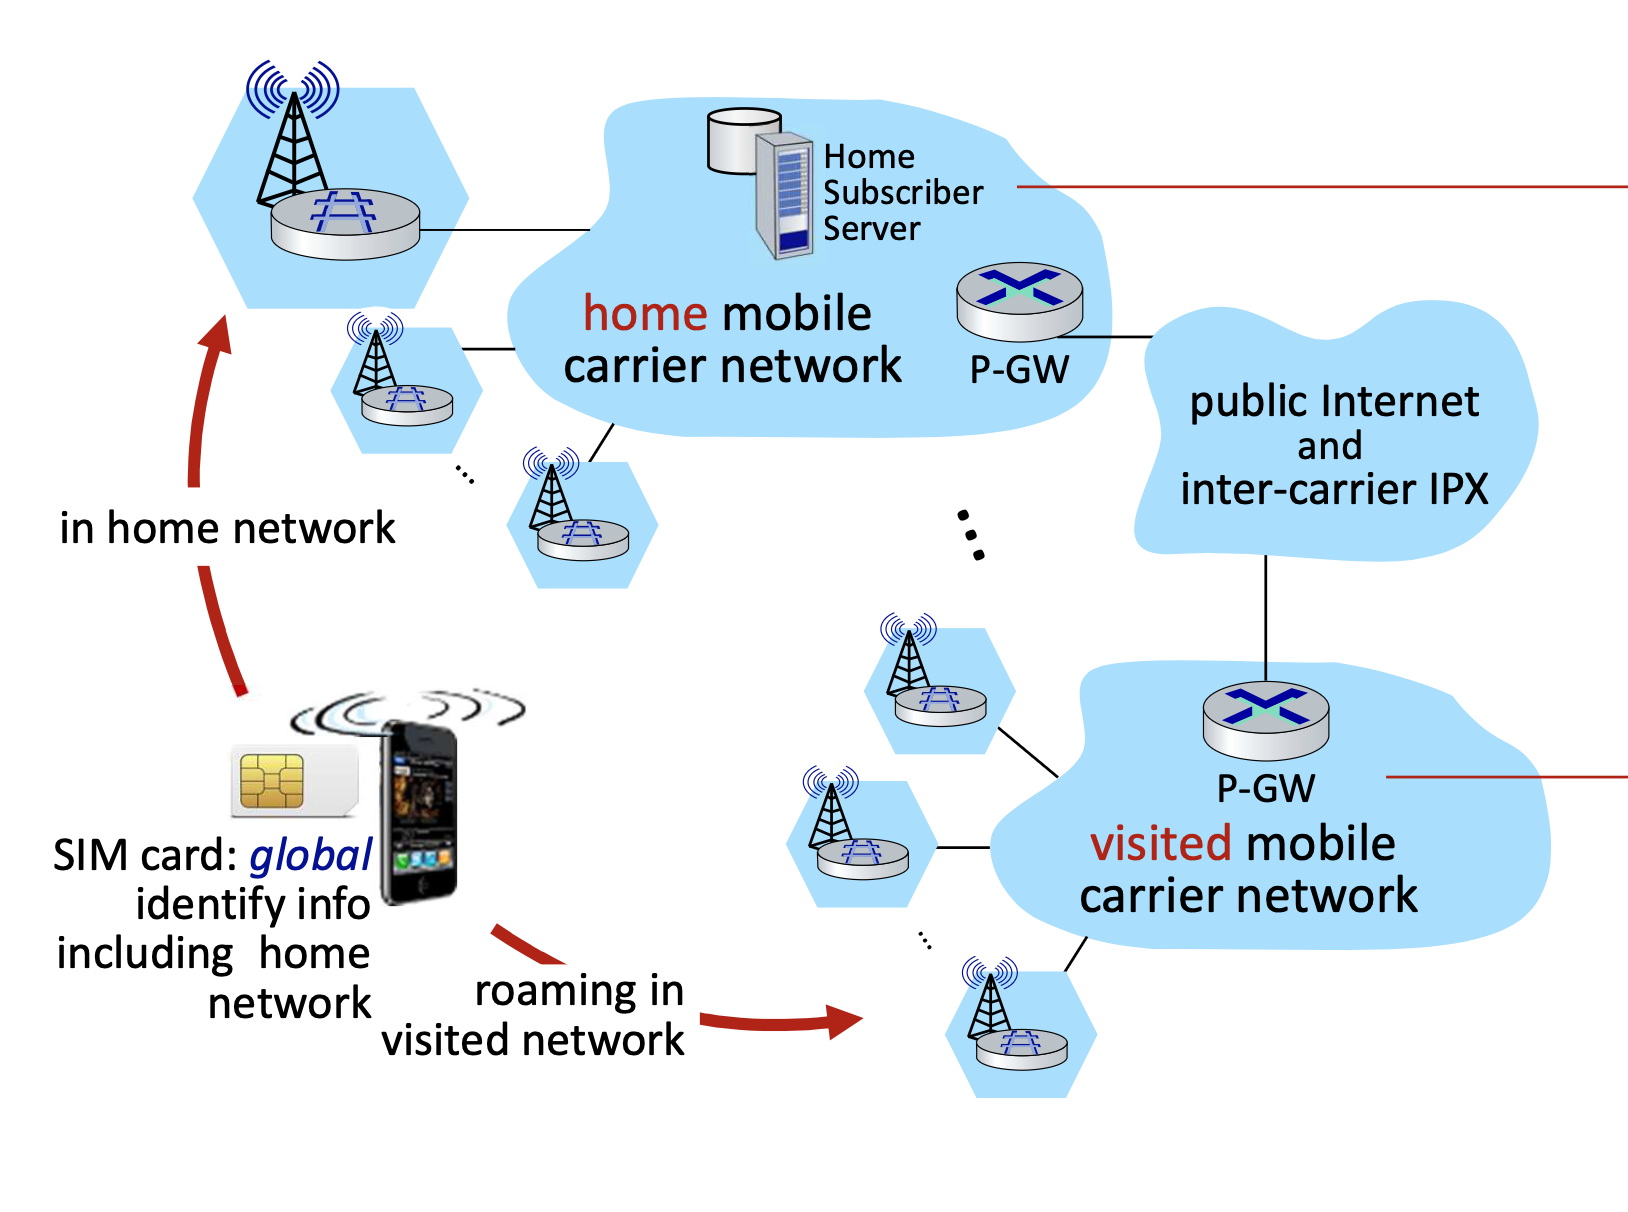
\includegraphics[keepaspectratio]{images/Screenshot-2026-03-10-alle-14-37-18.png}}
\caption{Struttura della home network in un'architettura 4G/5G.}
\end{figure}

Quando il dispositivo lascia la copertura del proprio operatore entra in
una \textbf{visited network}, condizione nota come \emph{roaming}. La
rete visitata ha accordi commerciali con altre reti per garantire
accesso ai dispositivi in transito.

\begin{figure}
\centering
\pandocbounded{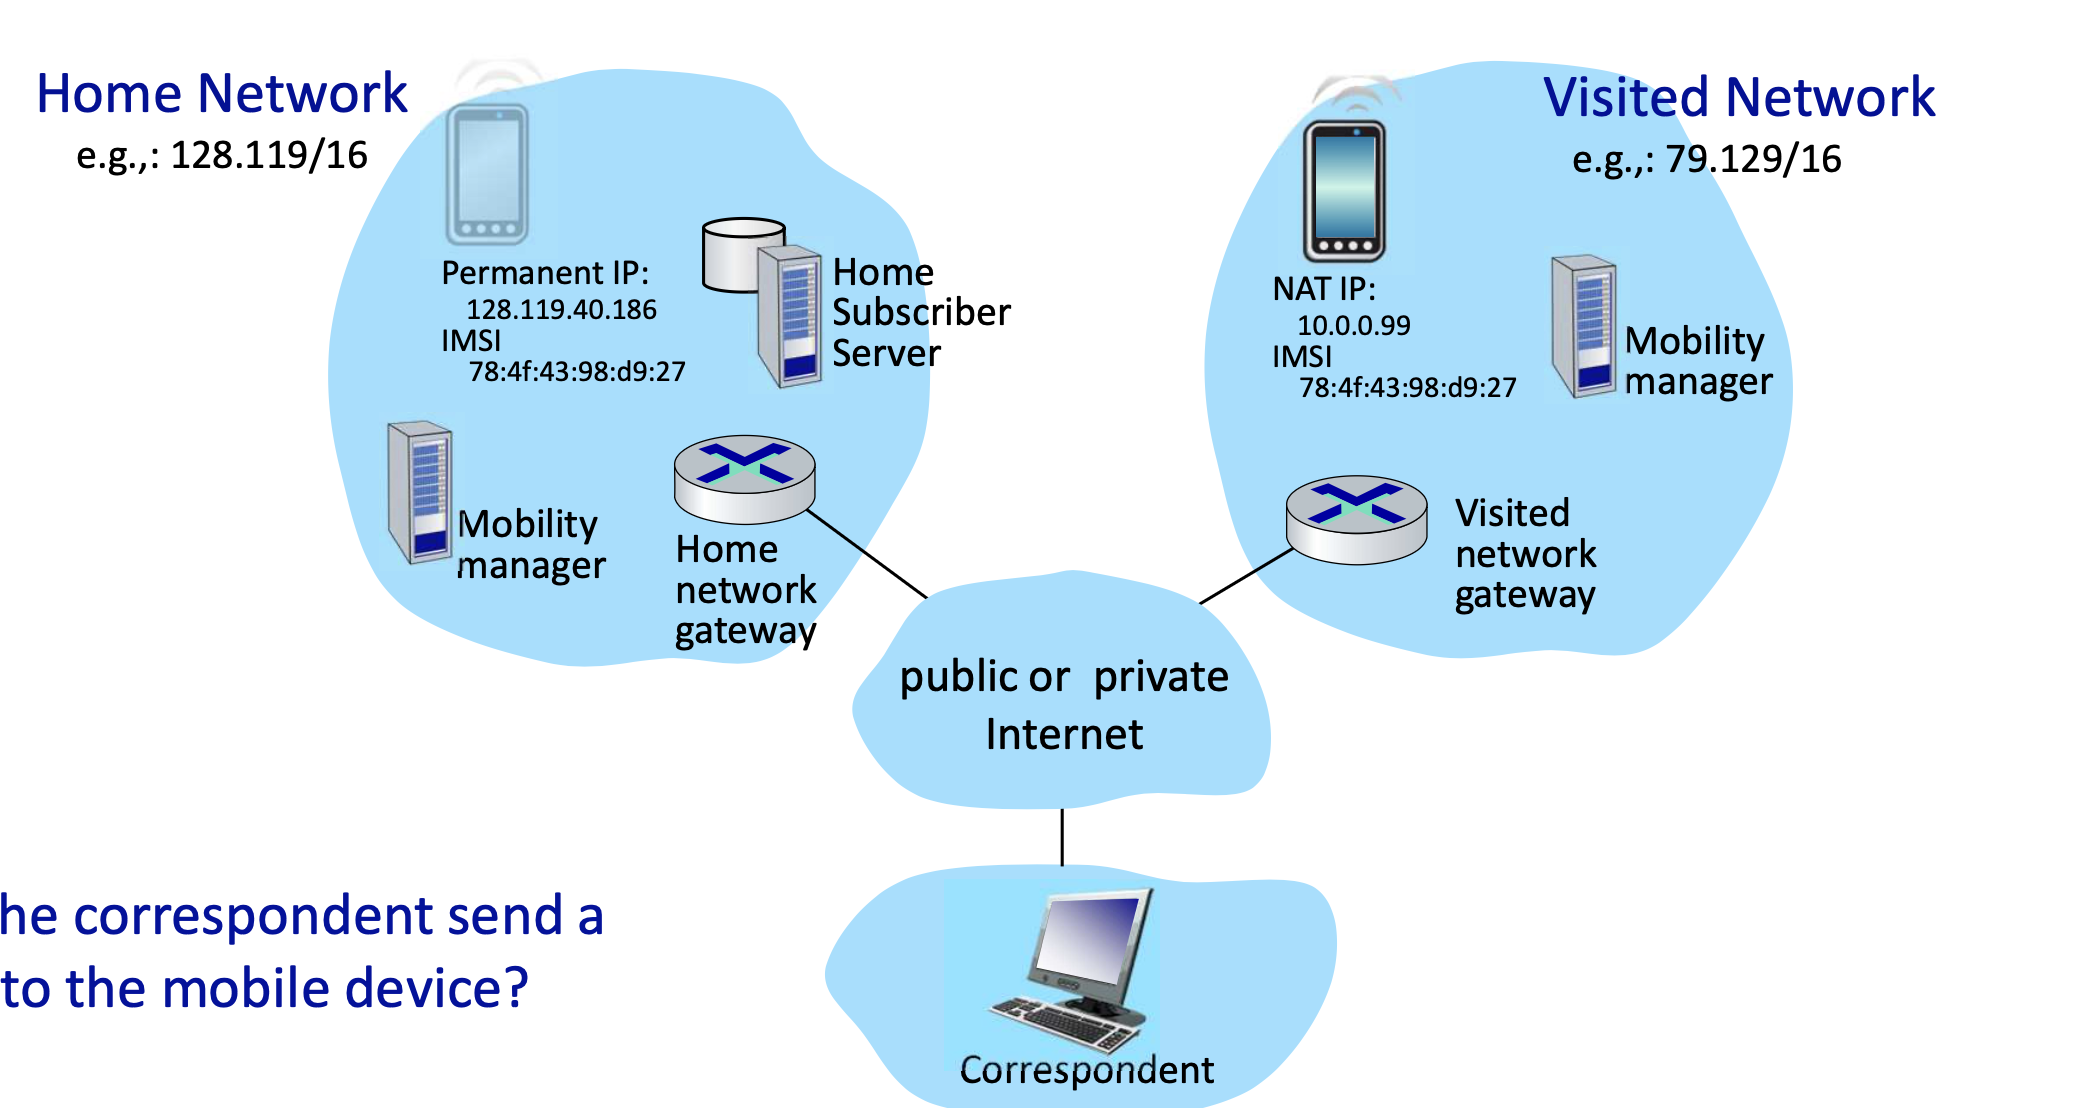
\includegraphics[keepaspectratio]{images/Pasted-image-20260313143711.png}}
\caption{Relazione tra home network e visited network in uno scenario di
roaming.}
\end{figure}

Le reti \textbf{ISP/WiFi} presentano un'architettura radicalmente
diversa: manca una nozione globale di home. L'autenticazione avviene
tramite server locali, le credenziali variano da rete a rete e la
mobilità fluida è difficile da realizzare. Esistono eccezioni
accademiche come \emph{eduroam} e architetture teoriche come
\textbf{Mobile IP}, ma quest'ultima non ha mai raggiunto un'adozione
commerciale significativa.

\begin{center}\rule{0.5\linewidth}{0.5pt}\end{center}

\section{Approcci alla Gestione della
Mobilità}\label{approcci-alla-gestione-della-mobilituxe0}

I progettisti di rete hanno valutato due filosofie principali per
permettere a un nodo corrispondente di raggiungere un dispositivo
mobile.

Il primo approccio affida la mobilità direttamente ai router, che
annuncerebbero la posizione del nodo mobile attraverso i consueti
protocolli di routing. Tecnicamente Internet potrebbe supportarlo
tramite il \emph{longest prefix match}, ma l'approccio è stato scartato
per mancanza di scalabilità: propagare la posizione di miliardi di
dispositivi mobili nelle tabelle di routing globali è impraticabile.

Il secondo approccio, quello effettivamente implementato, sposta la
complessità ai margini della rete (\emph{edge}), lasciando che siano i
sistemi terminali a gestirla. Questo dà origine a due tecniche: il
\textbf{routing indiretto} e il \textbf{routing diretto}.

\begin{center}\rule{0.5\linewidth}{0.5pt}\end{center}

\section{La Fase di Registrazione}\label{la-fase-di-registrazione}

Indipendentemente dalla tecnica di routing adottata, la home network
deve sempre conoscere la posizione corrente del dispositivo. Questo
avviene tramite la \textbf{registrazione}: il dispositivo si associa a
un \emph{mobility manager} nella rete visitata, il quale comunica la
posizione aggiornata all'HSS domestico. Al termine della procedura, il
mobility manager della rete visitata è a conoscenza della presenza del
dispositivo e l'HSS domestico conosce la sua posizione remota.

\begin{figure}
\centering
\pandocbounded{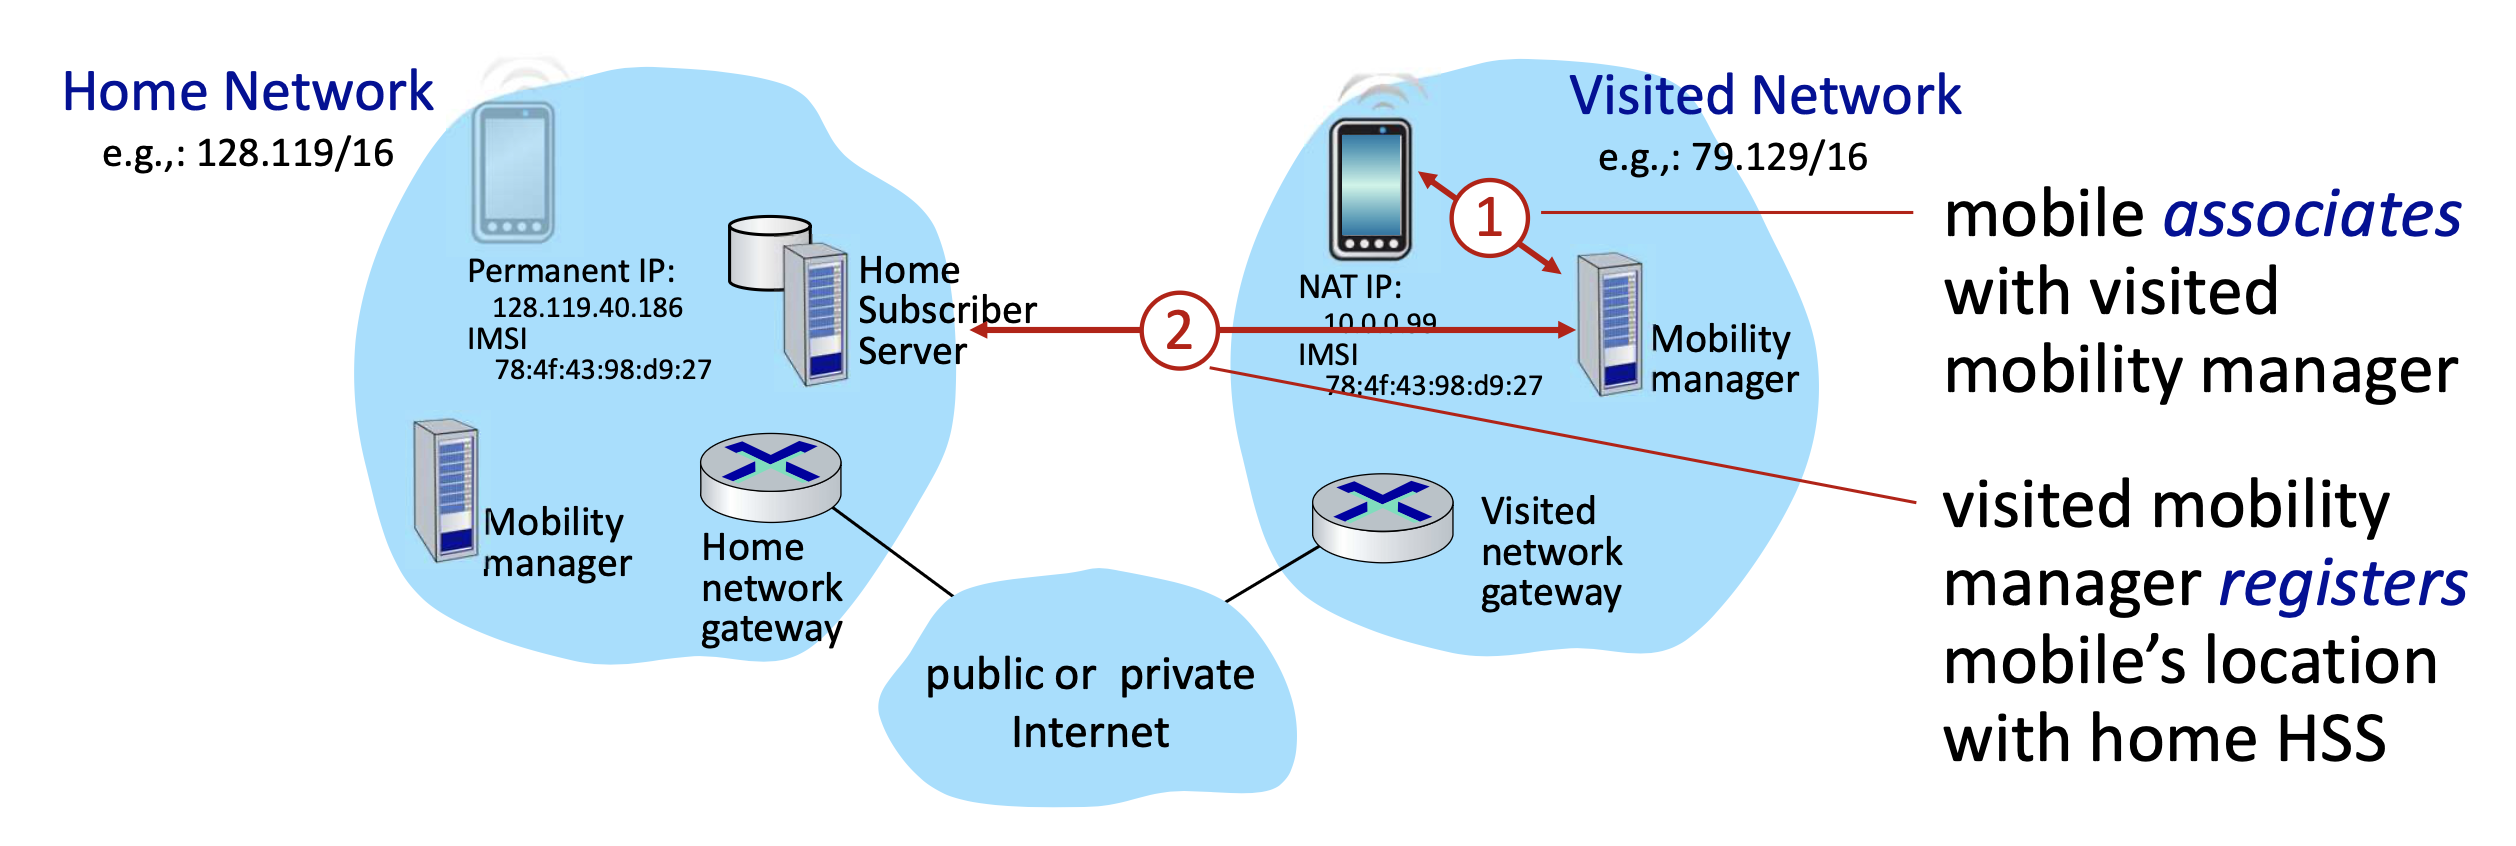
\includegraphics[keepaspectratio]{images/Pasted-image-20260313143813.png}}
\caption{Procedura di registrazione tra visited network e home network.}
\end{figure}

Durante le operazioni in roaming il dispositivo mantiene il proprio
indirizzo permanente associato alla home network, ma ottiene
temporaneamente un indirizzo IP nel range della rete visitata,
tipicamente assegnato tramite NAT.

\begin{center}\rule{0.5\linewidth}{0.5pt}\end{center}

\section{Routing Indiretto e Routing
Diretto}\label{routing-indiretto-e-routing-diretto}

Nel \textbf{routing indiretto} --- modalità standard per le reti 4G LTE
e per Mobile IP --- il nodo corrispondente invia il datagramma
all'indirizzo permanente del dispositivo mobile. Il gateway della home
network lo riceve, lo incapsula in un tunnel e lo inoltra al gateway
della rete visitata, che decapsula il pacchetto, applica la traduzione
NAT e lo consegna al dispositivo. Le risposte possono seguire il
percorso inverso oppure essere inviate direttamente al corrispondente.

Perché questo meccanismo funzioni servono tre protocolli specifici:

\begin{enumerate}
\def\labelenumi{\arabic{enumi}.}
\tightlist
\item
  \textbf{Protocollo di associazione} dispositivo--rete visitata: il
  dispositivo si associa alla rete visitata e si disassocia quando la
  lascia.
\item
  \textbf{Protocollo di registrazione} rete visitata--HSS domestico: la
  rete visitata comunica all'HSS la posizione del dispositivo.
\item
  \textbf{Protocollo di tunneling} tra i due gateway: il gateway
  domestico incapsula il datagramma originale; il gateway visitato lo
  decapsula, applica il NAT e lo consegna al dispositivo.
\end{enumerate}

Questo schema genera il cosiddetto \emph{triangle routing}: se
corrispondente e dispositivo si trovano nella stessa rete, i dati
compiono un percorso inutilmente lungo fino alla home network. Il
vantaggio, però, è notevole: ogni cambio di rete visitata è
completamente trasparente per il corrispondente --- la nuova rete si
registra presso l'HSS e il traffico viene reindirizzato nel nuovo tunnel
senza azioni da parte del corrispondente.

\begin{calloutnote}{Continuità delle sessioni durante il cambio di rete}

Quando il dispositivo si sposta in una nuova rete visitata, possono
andare persi alcuni datagrammi in transito. Tuttavia le sessioni TCP
rimangono attive: dal punto di vista del corrispondente, la posizione
del mobile è un dettaglio interno alla home network.

\end{calloutnote}

Nel \textbf{routing diretto} il corrispondente interroga l'HSS domestico
per ottenere il \emph{care-of-address} del dispositivo nella rete
visitata e invia i datagrammi direttamente a quell'indirizzo, eliminando
le inefficienze del triangle routing. Tuttavia l'approccio non è
trasparente per il corrispondente, che deve gestire esplicitamente la
richiesta dell'indirizzo. Inoltre, se il dispositivo cambia rete durante
una sessione attiva, il problema è più complesso: il corrispondente ha
interrogato l'HSS \textbf{solo all'inizio della sessione} e non conosce
il nuovo indirizzo; sono quindi necessari meccanismi aggiuntivi per
aggiornare dinamicamente il flusso dati, a differenza del routing
indiretto dove è sufficiente cambiare l'endpoint del tunnel.

\begin{center}\rule{0.5\linewidth}{0.5pt}\end{center}

\section{L'Architettura Pratica: Mobilità nelle Reti
4G}\label{larchitettura-pratica-mobilituxe0-nelle-reti-4g}

Quando un dispositivo entra in una rete 4G visitata, la gestione della
mobilità si sviluppa attraverso quattro fasi distinte che coinvolgono
progressivamente il piano di controllo, il piano dati e infine la
transizione tra celle.

\begin{itemize}
\item
  Il punto di ingresso è l'\textbf{associazione alla Base Station (BS)}:
  il dispositivo si aggancia alla stazione radio base della rete
  visitata e si identifica tramite il proprio \textbf{IMSI}
  (\emph{International Mobile Subscriber Identity}), che codifica sia
  l'identità del dispositivo sia la sua home network di appartenenza.
\item
  A questo punto entra in gioco il \textbf{piano di controllo}: la BS
  coinvolge la \textbf{Mobility Management Entity (MME)} locale, che usa
  l'IMSI per contattare l'HSS domestico. L'HSS restituisce all'MME i
  parametri di autenticazione, crittografia e servizi abilitati per
  quell'utente, e al tempo stesso viene aggiornato sulla nuova posizione
  del dispositivo. È qui che avviene la registrazione vera e propria: da
  questo momento l'HSS domestico sa dove si trova l'utente.
\item
  Una volta autenticato l'utente, l'MME configura il \textbf{piano dati}
  stabilendo i tunnel necessari a far fluire il traffico. Poiché si
  adotta routing indiretto, tutto il traffico deve transitare per la
  home network. Vengono creati due tunnel distinti, entrambi usando il
  protocollo \textbf{GTP} (\emph{GPRS Tunneling Protocol}):

  \begin{itemize}
  \tightlist
  \item
    \textbf{Tunnel BS ↔ S-GW}: quando il dispositivo cambia Base
    Station, non occorre ricreare il tunnel --- è sufficiente aggiornare
    l'indirizzo IP dell'endpoint sul lato BS.
  \item
    \textbf{Tunnel S-GW ↔ P-GW} (home network): implementa il routing
    indiretto verso la home network.
  \end{itemize}
\item
  La quarta fase è l'\textbf{handover tra Base Station}, che si attiva
  quando il dispositivo si sposta e la qualità del segnale sulla BS
  corrente degrada. La procedura completa si articola in sette passi:

  \begin{enumerate}
  \def\labelenumi{\arabic{enumi}.}
  \tightlist
  \item
    La \textbf{BS sorgente} decide di avviare l'handover (per degrado
    del segnale o sovraccarico) e seleziona la \emph{target BS},
    inviandole una \textbf{Handover Request}.
  \item
    La \textbf{target BS} pre-alloca le risorse radio e risponde con un
    \textbf{Handover Request ACK} contenente le informazioni di
    configurazione per il dispositivo.
  \item
    La \textbf{BS sorgente} notifica il dispositivo del cambio
    imminente; da questo momento il dispositivo può già trasmettere
    tramite la nuova BS --- l'handover sembra completato dal punto di
    vista del dispositivo.
  \item
    La \textbf{BS sorgente} smette di trasmettere al dispositivo e
    inizia a \textbf{forwardare} i datagrammi in arrivo verso la target
    BS (che li recapita al dispositivo via radio).
  \item
    La \textbf{target BS} informa l'\textbf{MME} di essere la nuova BS
    per il dispositivo.
  \item
    L'\textbf{MME} istruisce lo \textbf{S-GW} di aggiornare l'endpoint
    del tunnel dati alla nuova target BS. La BS sorgente riceve conferma
    e può liberare le proprie risorse radio.
  \item
    I datagrammi del dispositivo fluiscono ora attraverso il
    \textbf{nuovo tunnel} dalla target BS allo S-GW.
  \end{enumerate}
\end{itemize}

\begin{callouttip}{Perché la BS sorgente decide l’handover}

Sia la decisione di avviare l'handover sia la scelta della target BS
spettano alla \textbf{BS sorgente} (non all'MME). L'MME viene coinvolto
solo nella fase finale per aggiornare il piano dati. Questo è un punto
frequente nelle domande d'esame.

\end{callouttip}

\begin{figure}
\centering
\pandocbounded{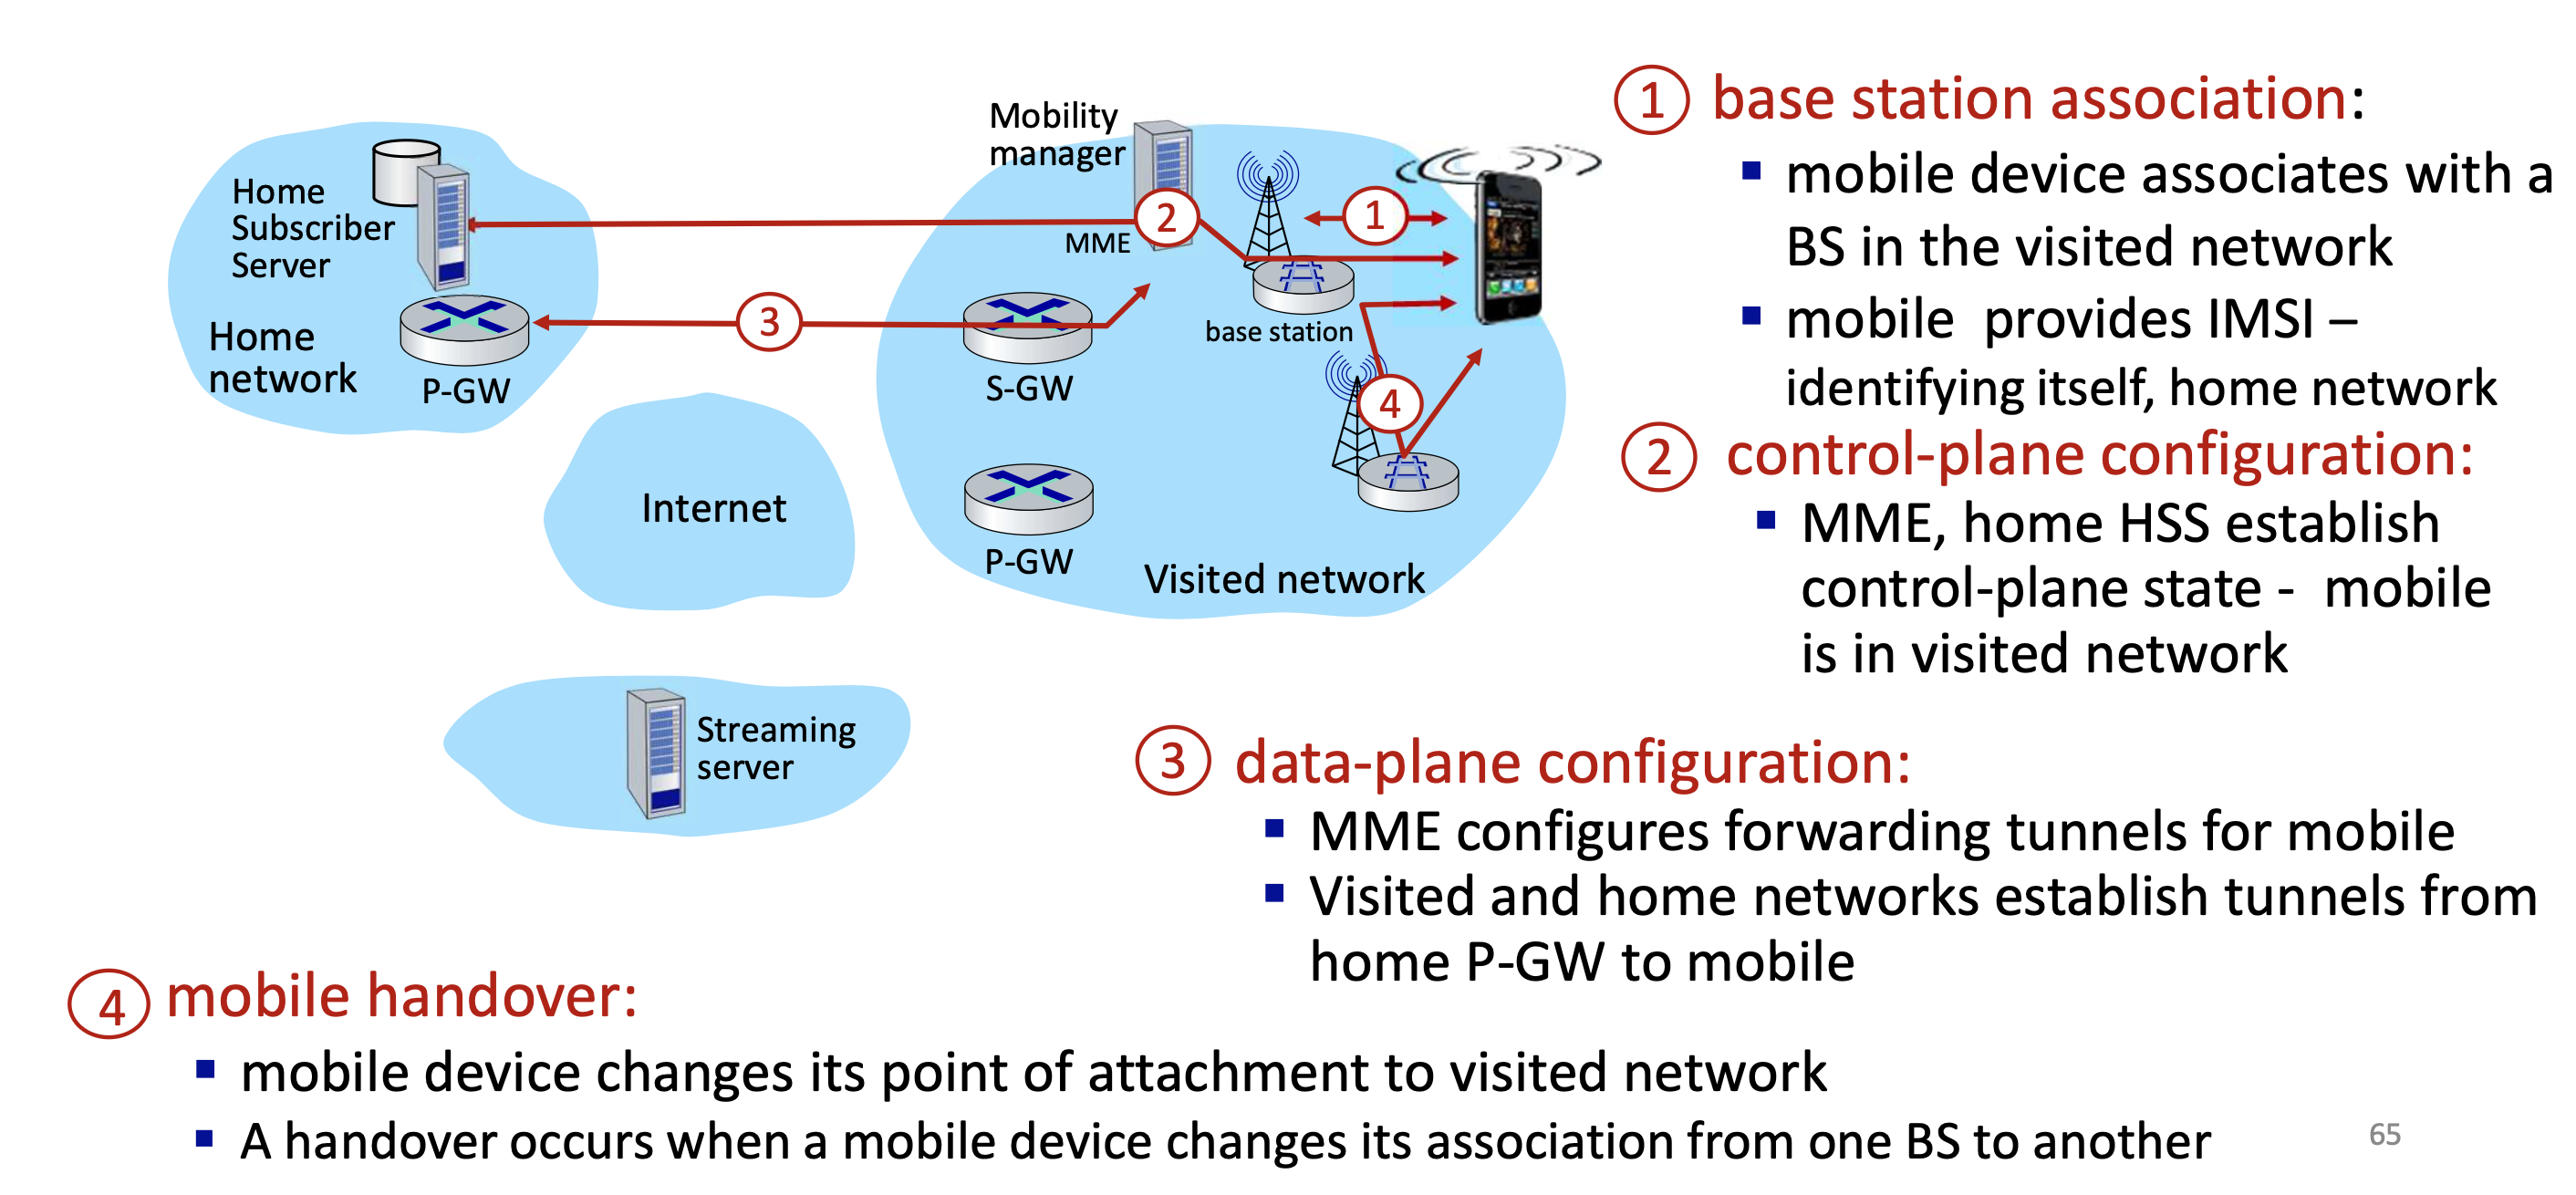
\includegraphics[keepaspectratio]{images/Pasted-image-20260313145859.png}}
\caption{Sequenza di messaggi durante un handover tra due Base Station
in 4G.}
\end{figure}

\begin{center}\rule{0.5\linewidth}{0.5pt}\end{center}

\section{Mobile IP e Impatto sui Protocolli di
Trasporto}\label{mobile-ip-e-impatto-sui-protocolli-di-trasporto}

L'architettura \textbf{Mobile IP} (RFC 5944), standardizzata circa
vent'anni fa, anticipava molti dei concetti oggi presenti nel 4G: il
\emph{home agent} univa i ruoli dell'attuale HSS e P-GW, mentre il
\emph{foreign agent} corrispondeva all'accoppiata MME/S-GW. La
registrazione avveniva tramite estensioni ICMP. All'epoca WiFi per i
dati e reti 2G/3G per la voce erano considerati sufficienti, e Mobile IP
non ha mai raggiunto una diffusione commerciale rilevante.

Sul fronte dell'impatto sui protocolli superiori, in teoria il layer
wireless dovrebbe essere trasparente: il modello \emph{best-effort} di
IP rimane invariato e TCP/UDP girano regolarmente su reti mobili. In
pratica le prestazioni degradano sensibilmente. Errori di bit sui link
radio e interruzioni transitorie durante gli handover vengono
interpretati da TCP come sintomi di congestione di rete, inducendolo a
ridurre la \emph{congestion window} in modo ingiustificato. A questo si
aggiungono la limitatezza di banda dei link wireless e i ritardi che
penalizzano il traffico in tempo reale.

\begin{center}\rule{0.5\linewidth}{0.5pt}\end{center}

\newpage

\chapter{Software Defined Networking
(SDN)}\label{software-defined-networking-sdn}

Questo paradigma architetturale segna il definitivo passaggio da un
sistema di protocolli puramente distribuiti a un framework di controllo
di rete completamente programmabile.

\begin{calloutdefinition}{Software Defined Networking}

Il \textbf{Software Defined Networking} è un approccio alla gestione
delle reti che sfrutta potenti meccanismi di astrazione per abilitare
configurazioni e operazioni dinamiche ed efficienti a livello
programmatico. La caratteristica distintiva è la separazione netta tra
\textbf{control plane} e \textbf{data plane}.

\end{calloutdefinition}

\begin{center}\rule{0.5\linewidth}{0.5pt}\end{center}

\section{L'Evoluzione dei Requisiti e la Complessità del
Traffico}\label{levoluzione-dei-requisiti-e-la-complessituxe0-del-traffico}

Sebbene il SDN sia spesso definito come un'idea radicalmente nuova, esso
nasce per risolvere problemi concreti dettati dai moderni trend
tecnologici: l'esplosione del \textbf{Cloud computing}, la gestione dei
\textbf{Big data}, il massiccio aumento del traffico mobile e la
diffusione pervasiva dell'\textbf{IoT} (Internet of Things). I
dispositivi moderni possiedono CPU più potenti, buffer più capienti e
link più veloci, ma il vero ostacolo non risiede nei puri volumi di
traffico, bensì nella sua \textbf{variabilità spaziale e temporale}: i
pattern di traffico sono diventati altamente dinamici, complessi e
strettamente sensibili alle applicazioni che li generano, rendendo
insufficiente la gestione statica.

La complessità e dinamicità del traffico sono alimentate da tre fenomeni
strutturali. Le architetture applicative moderne sono fortemente
distribuite: interrogano database multipli e server di backend,
generando enormi volumi di traffico orizzontale tra server che si
sommano al tradizionale traffico verticale client-server. La
proliferazione di piattaforme di \textbf{Unified Communications (UC)}
integra su un'unica infrastruttura servizi come chat, voce, video e
gestione della presenza, obbligando la rete a sostenere flussi paralleli
con requisiti di \textbf{QoS} radicalmente diversi. Infine, l'ascesa del
cloud computing ha alterato la località geografica del traffico: dati un
tempo confinati nel perimetro aziendale oggi attraversano ampie
\textbf{WAN} verso cloud remoti, sottoponendo i router enterprise a
carichi severi e imprevedibili.

La virtualizzazione aggrava ulteriormente il quadro: migrazioni,
replicazioni e failover di \textbf{Virtual Machines} causano forti
sbalzi di traffico orizzontale la cui posizione e intensità variano
costantemente. I dispositivi mobili aggiungono frequenti cambi di access
point e ritmi di utilizzo irregolari. Il risultato è che applicazioni
real-time necessitano bassa latenza, backup di massa privilegiano la
banda, e transazioni finanziarie richiedono garanzie di consegna ---
esigenze incompatibili con l'instradamento statico.

\begin{calloutnote}{Il dominio del traffico East-West}

Oltre il 70\% del traffico di rete odierno è di natura
\textbf{East-West}, ovvero circoscritto alle comunicazioni interne tra
server all'interno di un data center. I tradizionali data center a tre
livelli (Access, Aggregation, Core) sono però ottimizzati per il
traffico \textbf{North-South} (richieste client-server). Gestire
efficientemente il traffico East-West richiede selezione
ultra-flessibile dei path, load balancing efficace e riconfigurazioni
immediate.

\end{calloutnote}

\begin{center}\rule{0.5\linewidth}{0.5pt}\end{center}

\section{Limiti Strutturali delle Architetture
Tradizionali}\label{limiti-strutturali-delle-architetture-tradizionali}

Le reti convenzionali falliscono di fronte ai moderni scenari per tre
ragioni fondamentali. L'\textbf{architettura statica e frammentata} è il
primo problema: ogni protocollo risolve un problema isolato (routing,
spanning tree, ACL) moltiplicando la complessità operativa senza una
visione globale. L'\textbf{incoerenza delle policy} è il secondo: i
parametri vengono elaborati localmente, obbligando gli operatori ad
aggiornare manualmente ogni dispositivo con alto rischio di errata
configurazione. Il \textbf{vendor lock-in} è il terzo: la logica di
controllo è incapsulata in hardware proprietario privo di interfacce
aperte, che impedisce la programmabilità dell'infrastruttura.

La forza storica di Internet è stata l'architettura a livelli gerarchici
(Fisico, Link, Rete, Trasporto, Applicazione): la suddivisione in strati
fornisce astrazioni precise dei servizi e consente a ciascun livello di
evolversi indipendentemente. Tuttavia, queste astrazioni non sono state
applicate in egual misura a tutti i piani. Mentre il data plane gode di
logiche definite, il \textbf{control plane} tradizionale si è evoluto
caoticamente aggiungendo protocolli su protocolli a ogni nuovo requisito
tecnico. Costruito attorno a hardware chiusi con interfacce
proprietarie, il network management non segue i principi solidi
adottati, ad esempio, nei sistemi di database distribuiti: il risultato
è un groviglio ingestibile di regole che sopprime l'innovazione.

\begin{center}\rule{0.5\linewidth}{0.5pt}\end{center}

\section{La Separazione tra Data Plane e Control
Plane}\label{la-separazione-tra-data-plane-e-control-plane}

\begin{calloutdefinition}{Data Plane e Control Plane}

Il \textbf{Data Plane (Forwarding)} è l'atto meccanico e istantaneo di
smistare ogni singolo pacchetto in transito su una porta d'uscita del
router. Il \textbf{Control Plane (Routing)} è il processo decisionale,
su scale temporali molto più dilatate, attraverso cui si mappa il
tragitto completo sorgente-destinazione.

\end{calloutdefinition}

Nel tradizionale instradamento IP entrambi coesistono in un modello
\textbf{per-router control plane} fortemente accoppiato: gli algoritmi
risiedono in ogni nodo e calcolano localmente le tabelle di forwarding
in modo decentralizzato. Tale struttura fu ideata per garantire
resilienza, ma rende le moderne operazioni di \emph{Traffic Engineering}
estremamente difficili. I link weight sono l'unico ``manopola di
controllo'' disponibile. Si considerino tre scenari concreti su una rete
con nodi u, v, w, x, y, z:

\begin{callouttip}{Tre scenari impossibili con il routing tradizionale}

\textbf{Scenario 1 --- Percorso specifico}: l'operatore vuole che il
traffico da u a z segua il percorso u→v→w→z anziché il percorso più
breve u→x→y→z. L'unica leva è ridefinire i link weight affinché
l'algoritmo calcoli quella rotta --- ma non esiste garanzia che il
risultato sia quello voluto senza effetti collaterali sugli altri
flussi.

\textbf{Scenario 2 --- Load balancing}: l'operatore vuole dividere il
traffico da u a z equamente tra i due percorsi u→v→w→z e u→x→y→z. Non è
possibile con il routing basato su destinazione: l'algoritmo converge su
un unico percorso minimo.

\textbf{Scenario 3 --- Routing per-flusso}: il nodo w vuole instradare
verso z in modo diverso il traffico blu (proveniente da u) rispetto al
traffico rosso (proveniente da x). Non è possibile con il forwarding
basato sulla sola destinazione (LS, DV): la decisione dipende unicamente
dall'indirizzo di destinazione, non dal flusso.

\end{callouttip}

\begin{center}\rule{0.5\linewidth}{0.5pt}\end{center}

\section{Il Paradigma SDN: Centralizzazione Logica e
Programmabilità}\label{il-paradigma-sdn-centralizzazione-logica-e-programmabilituxe0}

La grande innovazione del SDN è il \textbf{Logically Centralized Control
Plane}: un controller interroga e supervisiona remotamente la topologia
globale calcolando le tabelle di forwarding per tutti i nodi. Mentre nel
modello classico ogni tabella è rigidamente calcolata come
\(T_{i} = SPF(Topology, link\_weights)\) ignorando metriche esterne, nel
modello SDN il controller calcola la funzione globale:

\[
\mathcal{F}: S(t) \rightarrow \{T_1, T_2, \ldots, T_n\}
\]

dove le tabelle di uscita derivano dallo stato \(S(t)\) che ingloba in
tempo reale topologia, traffico totale e vincoli di policy.

\begin{calloutimportant}{Architettura SDN e astrazione Match-Action}

Il SDN poggia su pilastri imprescindibili: una demarcazione netta tra
data plane e control plane; il control plane definisce il comportamento
strategico della rete mentre il data plane applica le direttive ai
pacchetti fisici; l'uso di switch elementari ad alte prestazioni
governati tramite l'astrazione \textbf{match-action} orientata ai flussi
(es. OpenFlow); il ricorso totale a protocolli aperti e programmabili.

\end{calloutimportant}

Il controller SDN comunica su due assi. La \textbf{Southbound API}
(tipicamente OpenFlow) è l'interfaccia verso il basso tra il controller
e gli switch del data plane, tramite cui vengono installate le regole di
forwarding nell'hardware. La \textbf{Northbound API} è l'interfaccia
verso l'alto che dialoga con le applicazioni di gestione (bilanciamento,
routing avanzato, access control), sviluppabili autonomamente da terze
parti indipendentemente dai produttori hardware.

\begin{calloutwarning}{L’illusione del server singolo}

Sebbene logicamente centralizzato, il \emph{SDN Controller} è
fisicamente implementato come un sistema fortemente distribuito. Ciò
assicura tolleranza agli errori, elevata scalabilità e robustezza contro
guasti singoli critici.

\end{calloutwarning}

\begin{center}\rule{0.5\linewidth}{0.5pt}\end{center}

\section{Architettura SDN: I Tre
Componenti}\label{architettura-sdn-i-tre-componenti}

L'architettura SDN si articola in tre livelli distinti con ruoli ben
separati.

\subsection{Data-Plane Switches}\label{data-plane-switches}

Gli switch del data plane sono dispositivi semplici e veloci, spesso
basati su hardware commodity a basso costo. Il loro unico compito è
applicare meccanicamente le regole di forwarding ai pacchetti in
transito secondo l'astrazione \textbf{match-action}: confrontano i campi
dell'intestazione del pacchetto con le regole nella flow table e
applicano l'azione corrispondente. Le flow table vengono calcolate e
installate da remoto dal controller, non localmente. Lo switch espone
un'API standardizzata (tipicamente OpenFlow) che definisce cosa è
controllabile dall'esterno e cosa no, e un protocollo per comunicare con
il controller.

\subsection{SDN Controller (Network Operating
System)}\label{sdn-controller-network-operating-system}

Il controller SDN svolge il ruolo di \textbf{sistema operativo di rete}:
mantiene una visione aggiornata dello stato globale della rete
(topologia, link attivi, tabelle di forwarding). È il punto di
mediazione tra le applicazioni che esprimono policy di alto livello e
gli switch che le devono applicare. Interagisce verso il basso tramite
la \textbf{Southbound API} con gli switch del data plane, e verso l'alto
tramite la \textbf{Northbound API} con le applicazioni di controllo.
Sebbene appaia come un'entità singola, è implementato come sistema
distribuito per garantire performance, scalabilità, tolleranza ai guasti
e robustezza.

\subsection{Network-Control
Applications}\label{network-control-applications}

Le applicazioni di controllo sono il vero ``cervello'' della rete:
implementano le funzioni di controllo (routing, access control, load
balancing, \ldots) sfruttando i servizi e le API esposte dal controller.
Il punto chiave è che sono \textbf{unbundled}: possono essere sviluppate
e fornite da soggetti terzi --- distinti sia dal produttore degli switch
hardware sia dal produttore del controller SDN. Questo disaccoppiamento
abilita un ecosistema aperto in cui l'innovazione a livello applicativo
è indipendente dall'hardware sottostante.

\begin{calloutnote}{Sintesi dell’architettura}

{\def\LTcaptype{none} % do not increment counter
\begin{longtable}[]{@{}
  >{\raggedright\arraybackslash}p{(\linewidth - 4\tabcolsep) * \real{0.3333}}
  >{\raggedright\arraybackslash}p{(\linewidth - 4\tabcolsep) * \real{0.4074}}
  >{\raggedright\arraybackslash}p{(\linewidth - 4\tabcolsep) * \real{0.2593}}@{}}
\toprule\noalign{}
\begin{minipage}[b]{\linewidth}\raggedright
Livello
\end{minipage} & \begin{minipage}[b]{\linewidth}\raggedright
Componente
\end{minipage} & \begin{minipage}[b]{\linewidth}\raggedright
Ruolo
\end{minipage} \\
\midrule\noalign{}
\endhead
\bottomrule\noalign{}
\endlastfoot
Alto & Network-control apps & ``Brains'': routing, load balancing, ACL
--- unbundled, terze parti \\
Medio & SDN Controller (Network OS) & Stato globale della rete;
northbound ↔ southbound \\
Basso & Data-plane switches & Match-action su flow table installate dal
controller \\
\end{longtable}
}

\end{calloutnote}

\begin{center}\rule{0.5\linewidth}{0.5pt}\end{center}

\section{Cronologia e Sviluppi
Storici}\label{cronologia-e-sviluppi-storici}

{\def\LTcaptype{none} % do not increment counter
\begin{longtable}[]{@{}
  >{\raggedright\arraybackslash}p{(\linewidth - 4\tabcolsep) * \real{0.3333}}
  >{\raggedright\arraybackslash}p{(\linewidth - 4\tabcolsep) * \real{0.3333}}
  >{\raggedright\arraybackslash}p{(\linewidth - 4\tabcolsep) * \real{0.3333}}@{}}
\toprule\noalign{}
\begin{minipage}[b]{\linewidth}\raggedright
\textbf{Periodo}
\end{minipage} & \begin{minipage}[b]{\linewidth}\raggedright
\textbf{Pietra Miliare}
\end{minipage} & \begin{minipage}[b]{\linewidth}\raggedright
\textbf{Dettagli}
\end{minipage} \\
\midrule\noalign{}
\endhead
\bottomrule\noalign{}
\endlastfoot
\textasciitilde2004 & Genesi ricercativa & Princeton, Stanford, Berkeley
avviano la ricerca su nuovi paradigmi di gestione del networking. \\
2008 & Nascita ufficiale SDN & NICIRA presenta NOX; OpenFlow nasce in
collaborazione con Stanford. \\
2011 & Standardizzazione & Fondazione dell'\textbf{Open Networking
Foundation (ONF)} con Google, Yahoo, Verizon, Cisco, HP, Dell. \\
2013 & Consacrazione scalabile & Picco di interesse all'Open Networking
Summit (1600 partecipanti). Google rende pubblica la propria
implementazione SDN sulla WAN globale. \\
2014 & Data center & VMware NSX e Cisco ACI portano SDN nei data center
globali. \\
2021+ & ML, 5G, P4 & Intent-Based Networking con AI/ML (Cisco DNA, Mist
AI). SDN come base del 5G. Linguaggio \textbf{P4} (Programming
Protocol-independent Packet Processors) per switch programmabili a line
speed. \\
\end{longtable}
}

\begin{center}\rule{0.5\linewidth}{0.5pt}\end{center}

\newpage

\chapter{Software Defined Networking (SDN) ---
Architettura}\label{software-defined-networking-sdn-architettura}

Il Software Defined Networking è un paradigma architetturale che separa
nettamente il \textbf{piano di controllo} (\emph{control plane}) dal
\textbf{piano dati} (\emph{data plane}). Questa separazione permette di
programmare il comportamento della rete in modo centralizzato,
eliminando la rigidità dei dispositivi di rete tradizionali che
incorporano sia la logica di instradamento che la funzione di
forwarding. La lezione approfondisce l'architettura interna di questi
due piani e i meccanismi con cui interagiscono.

\section{Motivazioni: Perché SDN?}\label{motivazioni-perchuxe9-sdn}

Il Software Defined Networking non è nato per risolvere un semplice
problema di capacità, ma per rispondere a una trasformazione strutturale
delle reti moderne. La domanda di rete --- alimentata da cloud
computing, big data, traffico mobile e IoT --- è cresciuta enormemente,
ma anche l'offerta ha tenuto il passo: CPU più veloci, buffer più
grandi, link ad alta capacità. Il vero problema, dunque, non è
quantitativo ma qualitativo: \textbf{la complessità si è spostata dal
volume alla variabilità}.

I pattern di traffico moderni sono \emph{time-variant} (cambiano nel
tempo), \emph{spatially dynamic} (cambiano nei percorsi) e
\emph{application-sensitive} (dipendono dal tipo di applicazione).
Questa variabilità richiede un controllo programmabile della rete, che
le architetture tradizionali non sono in grado di offrire.

\subsection{Dinamiche del Traffico
Moderno}\label{dinamiche-del-traffico-moderno}

Le applicazioni distribuite moderne accedono simultaneamente a
molteplici database e server backend, generando significativo traffico
``orizzontale'' (\emph{server-to-server}) in aggiunta al tradizionale
traffico ``verticale'' (\emph{client-server}). I servizi di Unified
Communications (UC) --- messaggistica, presenza, VoIP, videoconferenza
--- amplificano ulteriormente questa complessità, richiedendo alla rete
di supportare flussi concorrenti con requisiti di QoS eterogenei.

L'adozione massiva del cloud computing ha spostato traffico che un tempo
rimaneva all'interno delle reti enterprise verso data center remoti,
rendendo i carichi sui router enterprise imprevedibili. La
virtualizzazione dei server ha aggiunto un ulteriore strato: una singola
macchina fisica ospita multiple VM tra cui avvengono significative
comunicazioni (migrazione, replica, failover).

\begin{figure}
\centering
\pandocbounded{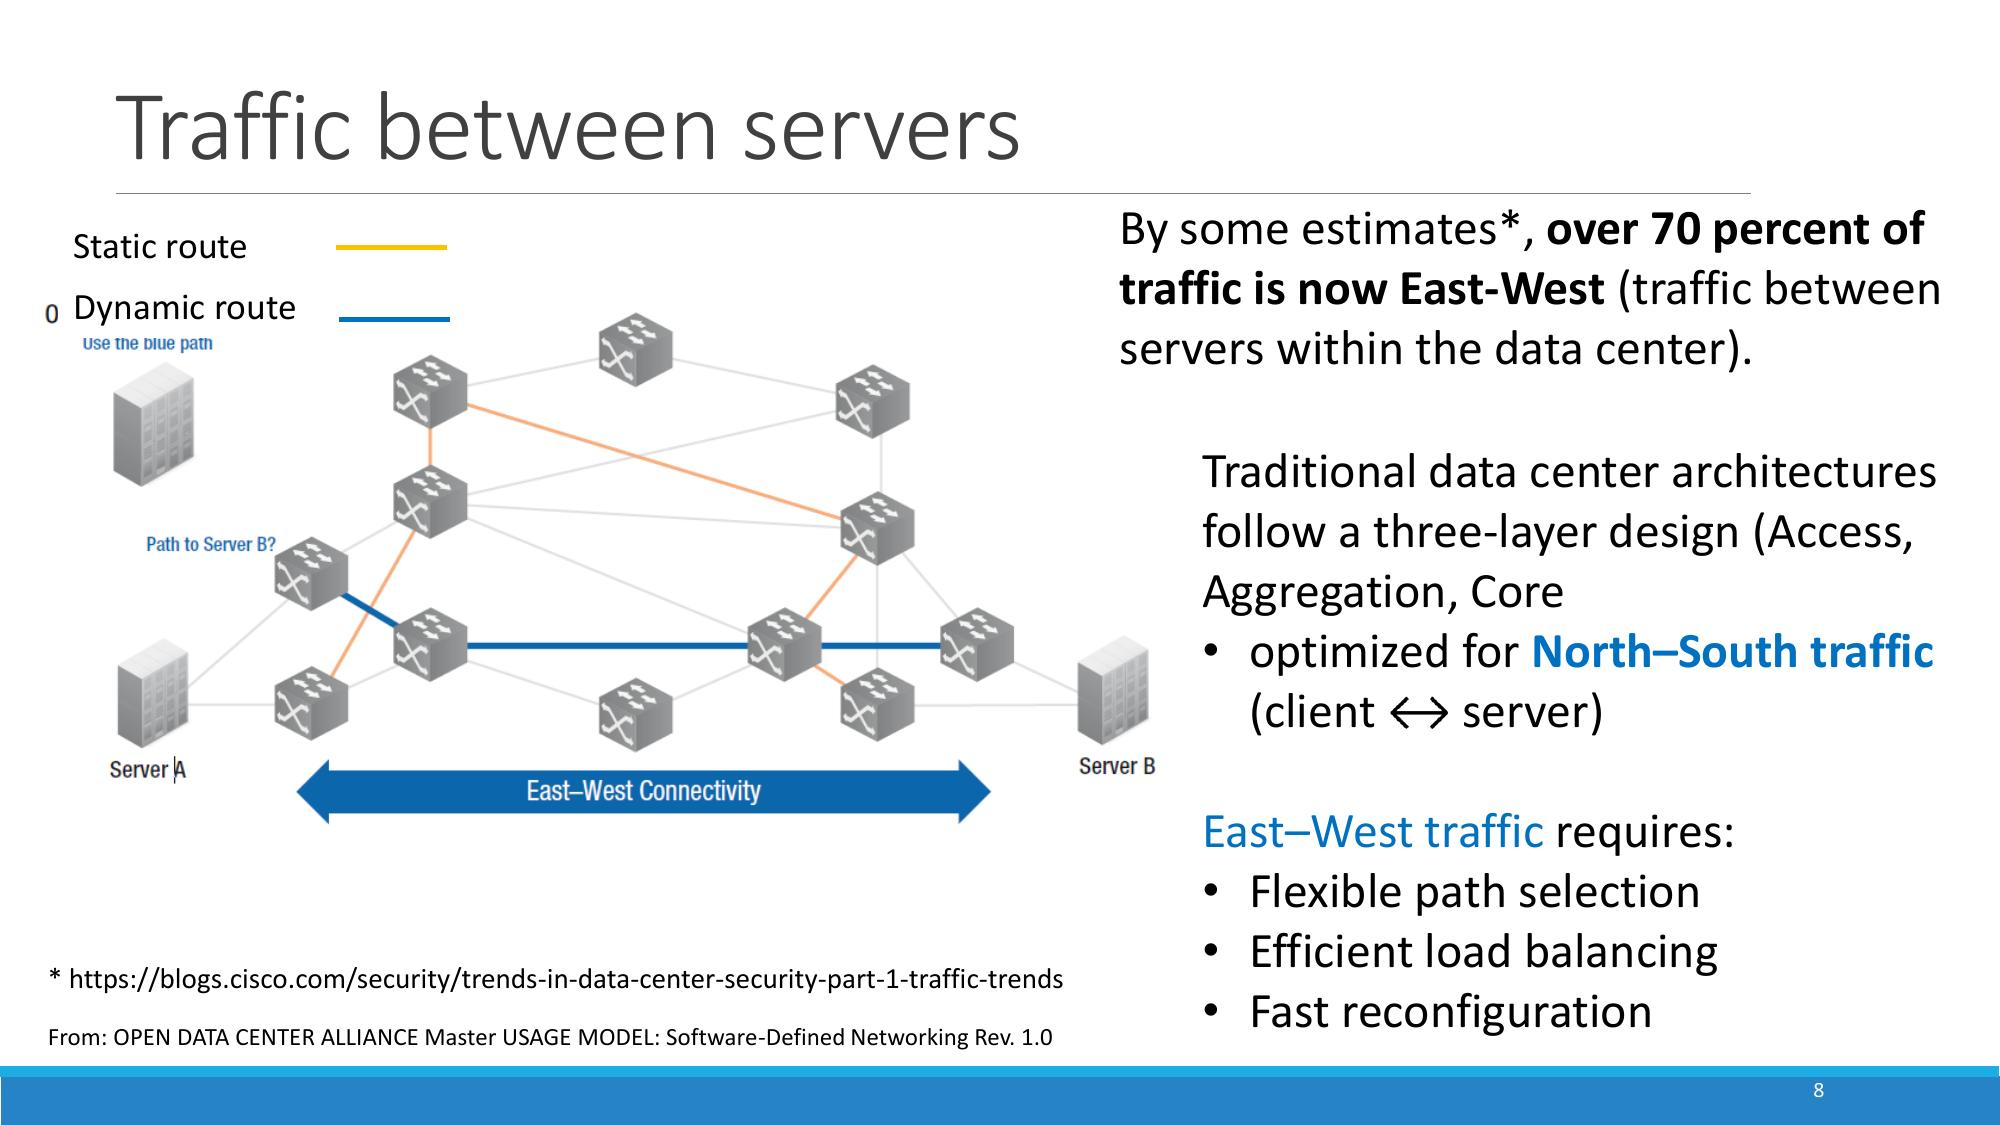
\includegraphics[keepaspectratio]{images/lezione-15-lab-sdn-architecture-img-01.jpg}}
\caption{0 --- Oltre il 70\% del traffico nei data center moderni è
East-West (tra server). Le architetture tradizionali a tre livelli
(Access, Aggregation, Core) erano ottimizzate per il traffico
North-South (client-server) e richiedono selezione flessibile dei
percorsi, load balancing efficiente e riconfigurazione rapida.}
\end{figure}

Il traffico mobile aggiunge un'ulteriore dimensione di imprevedibilità:
i dispositivi mobili generano carichi rapidamente mutevoli e cambiano
frequentemente il punto di connessione alla rete. Le applicazioni
moderne richiedono trattamento differenziato: le applicazioni real-time
(VoIP, videoconferenza) richiedono bassa latenza e alta priorità, mentre
i trasferimenti bulk (backup) richiedono ampia banda ma tollerano
ritardi.

\subsection{Limitazioni delle Reti
Tradizionali}\label{limitazioni-delle-reti-tradizionali}

Le tendenze descritte richiedono una gestione flessibile delle risorse
di rete, ma le architetture tradizionali mostrano tre limitazioni
strutturali:

\textbf{A) Architettura statica e complessa}: le reti tradizionali sono
costruite come collezione di protocolli indipendenti, ognuno pensato per
una funzione specifica e separata (routing, spanning tree, ACL, ecc.).
Il risultato è un control plane frammentato con complessità operativa
crescente.

\textbf{B) Inconsistenza delle policy e rigidità operativa}: le
modifiche di configurazione devono essere applicate manualmente su ogni
singolo dispositivo. Le policy vengono enforced localmente, non
globalmente, con alto rischio di misconfiguration.

\textbf{C) Dipendenza dal vendor e innovazione lenta}: la logica di
controllo è embedded in hardware proprietario, con interfacce chiuse.
Questo rende lento il deployment di nuovi servizi e limita la
programmabilità.

\begin{center}\rule{0.5\linewidth}{0.5pt}\end{center}

\section{Il Paradigma SDN}\label{il-paradigma-sdn}

\subsection{Separazione Control Plane / Data
Plane}\label{separazione-control-plane-data-plane}

Le funzioni di rete a livello network si dividono in due categorie
temporalmente molto diverse: il \textbf{forwarding} (spostare pacchetti
dall'input all'output appropriato) avviene su scala temporale dei
pacchetti (\emph{fast timescales}), mentre il \textbf{routing}
(determinare il percorso dei pacchetti da sorgente a destinazione)
avviene su scala degli eventi di controllo (\emph{slow timescales}). In
una rete tradizionale, queste due funzioni sono tightly coupled nello
stesso dispositivo.

\begin{calloutdefinition}{Software Defined Networking (SDN)}

Approccio alla gestione di rete che usa l'astrazione per abilitare una
configurazione e un'operazione della rete dinamica e programmaticamente
efficiente. Separa il control plane dal data plane, centralizzando
logicamente il primo in un controller remoto.

\end{calloutdefinition}

\subsubsection{Il Problema del Traffic Engineering
Tradizionale}\label{il-problema-del-traffic-engineering-tradizionale}

Nelle reti con routing distribuito, i router calcolano i percorsi
indipendentemente usando algoritmi come Dijkstra (link-state) o
Bellman-Ford (distance-vector). Il problema è che l'unico ``knob''
disponibile all'operatore sono i pesi dei link: se si vuole forzare il
traffico da u a z lungo il percorso uvwz invece di uxyz, bisogna
ricalcolare i pesi, e questo può influenzare altri flussi in modo
indesiderato.

\begin{figure}
\centering
\pandocbounded{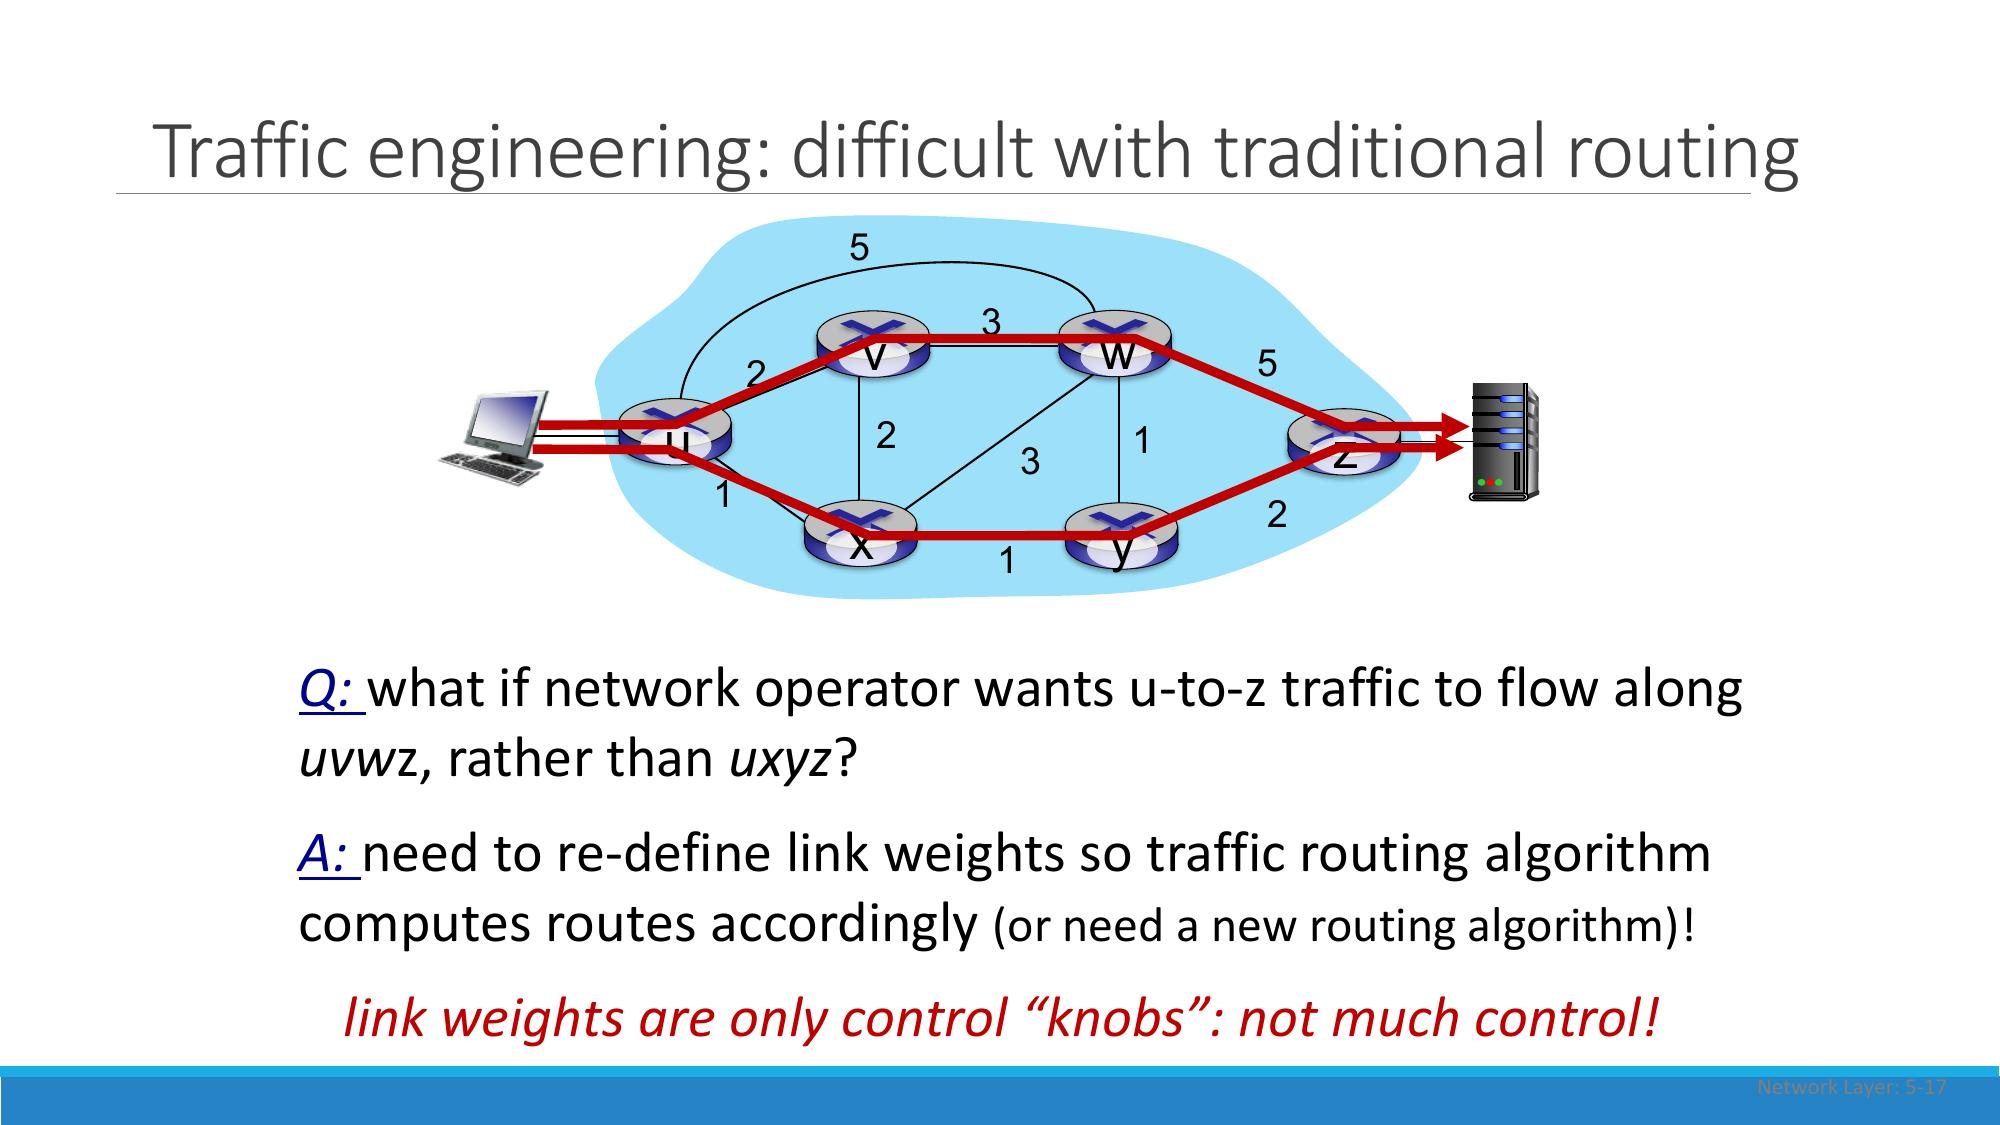
\includegraphics[keepaspectratio]{images/lezione-15-lab-sdn-architecture-img-02.jpg}}
\caption{0.1 --- Con il routing tradizionale, i link weights sono gli
unici ``knob'' di controllo. Non è possibile: (a) forzare percorsi
specifici senza alterare il routing globale, (b) fare load balancing su
più percorsi, (c) differenziare traffico di colori diversi sullo stesso
nodo.}
\end{figure}

SDN risolve questo problema spostando la logica di routing in un
controller centralizzato che ha visione globale della rete e può
installare regole arbitrarie in ogni switch.

\subsubsection{Control Plane Logicamente
Centralizzato}\label{control-plane-logicamente-centralizzato}

\begin{figure}
\centering
\pandocbounded{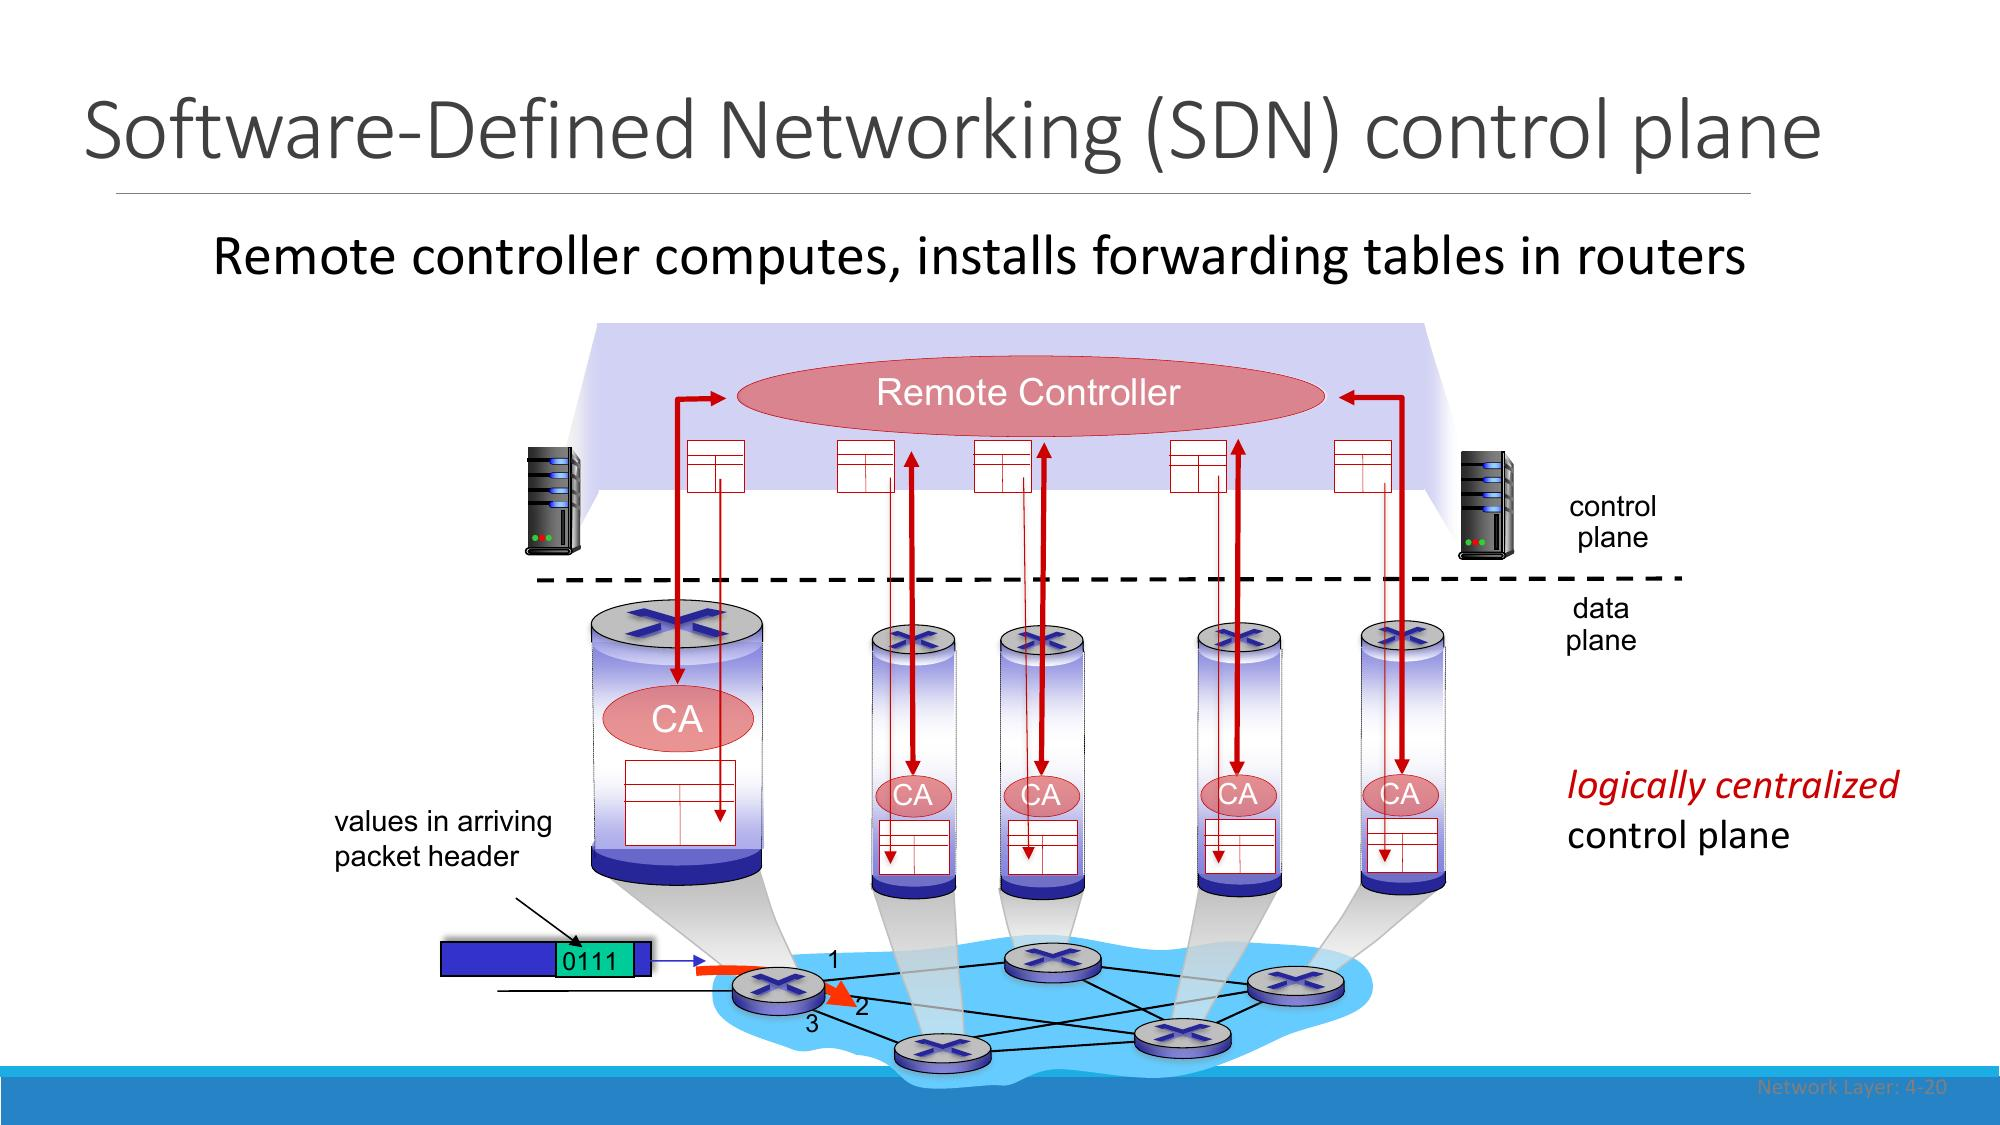
\includegraphics[keepaspectratio]{images/lezione-15-lab-sdn-architecture-img-03.jpg}}
\caption{0.2 --- Nel modello SDN, un Remote Controller logicamente
centralizzato calcola le forwarding table e le installa nei router. I
dispositivi del data plane (con etichetta CA, Controlled Agent) eseguono
le istruzioni ricevute senza logica di routing autonoma.}
\end{figure}

In una rete tradizionale, ogni router calcola la propria forwarding
table come: \[T_i = \text{SPF}(\text{Topology}, \text{link weights})\]
Il comportamento globale emerge da computazioni locali non coordinate.
Non vengono considerati la traffic demand (traffic matrix) né le policy
applicative.

In SDN, un controller centralizzato calcola:
\[\mathcal{F}: S(t) \rightarrow \{T_1, T_2, \ldots, T_n\}\] dove
\(S(t)\) include topologia, stato del traffico e policy. Le forwarding
table vengono calcolate in modo \textbf{consistente} su tutta la rete.

\subsubsection{I Quattro Pilastri di
SDN}\label{i-quattro-pilastri-di-sdn}

SDN si fonda su quattro idee principali:

\begin{enumerate}
\def\labelenumi{\arabic{enumi}.}
\tightlist
\item
  \textbf{Generalized flow-based forwarding}: il forwarding non si basa
  solo sull'indirizzo IP di destinazione, ma può usare qualsiasi campo
  dell'header (OpenFlow)
\item
  \textbf{Separazione control plane / data plane}: i dispositivi del
  data plane eseguono il forwarding senza prendere decisioni di routing
  autonome
\item
  \textbf{Control plane esterno agli switch}: la logica di controllo
  risiede nel controller, non nei dispositivi di rete
\item
  \textbf{Programmabilità}: le applicazioni di controllo implementano
  funzioni di rete (routing, access control, load balancing) usando le
  API del controller
\end{enumerate}

\subsection{Architettura SDN a Tre
Livelli}\label{architettura-sdn-a-tre-livelli}

\begin{figure}
\centering
\pandocbounded{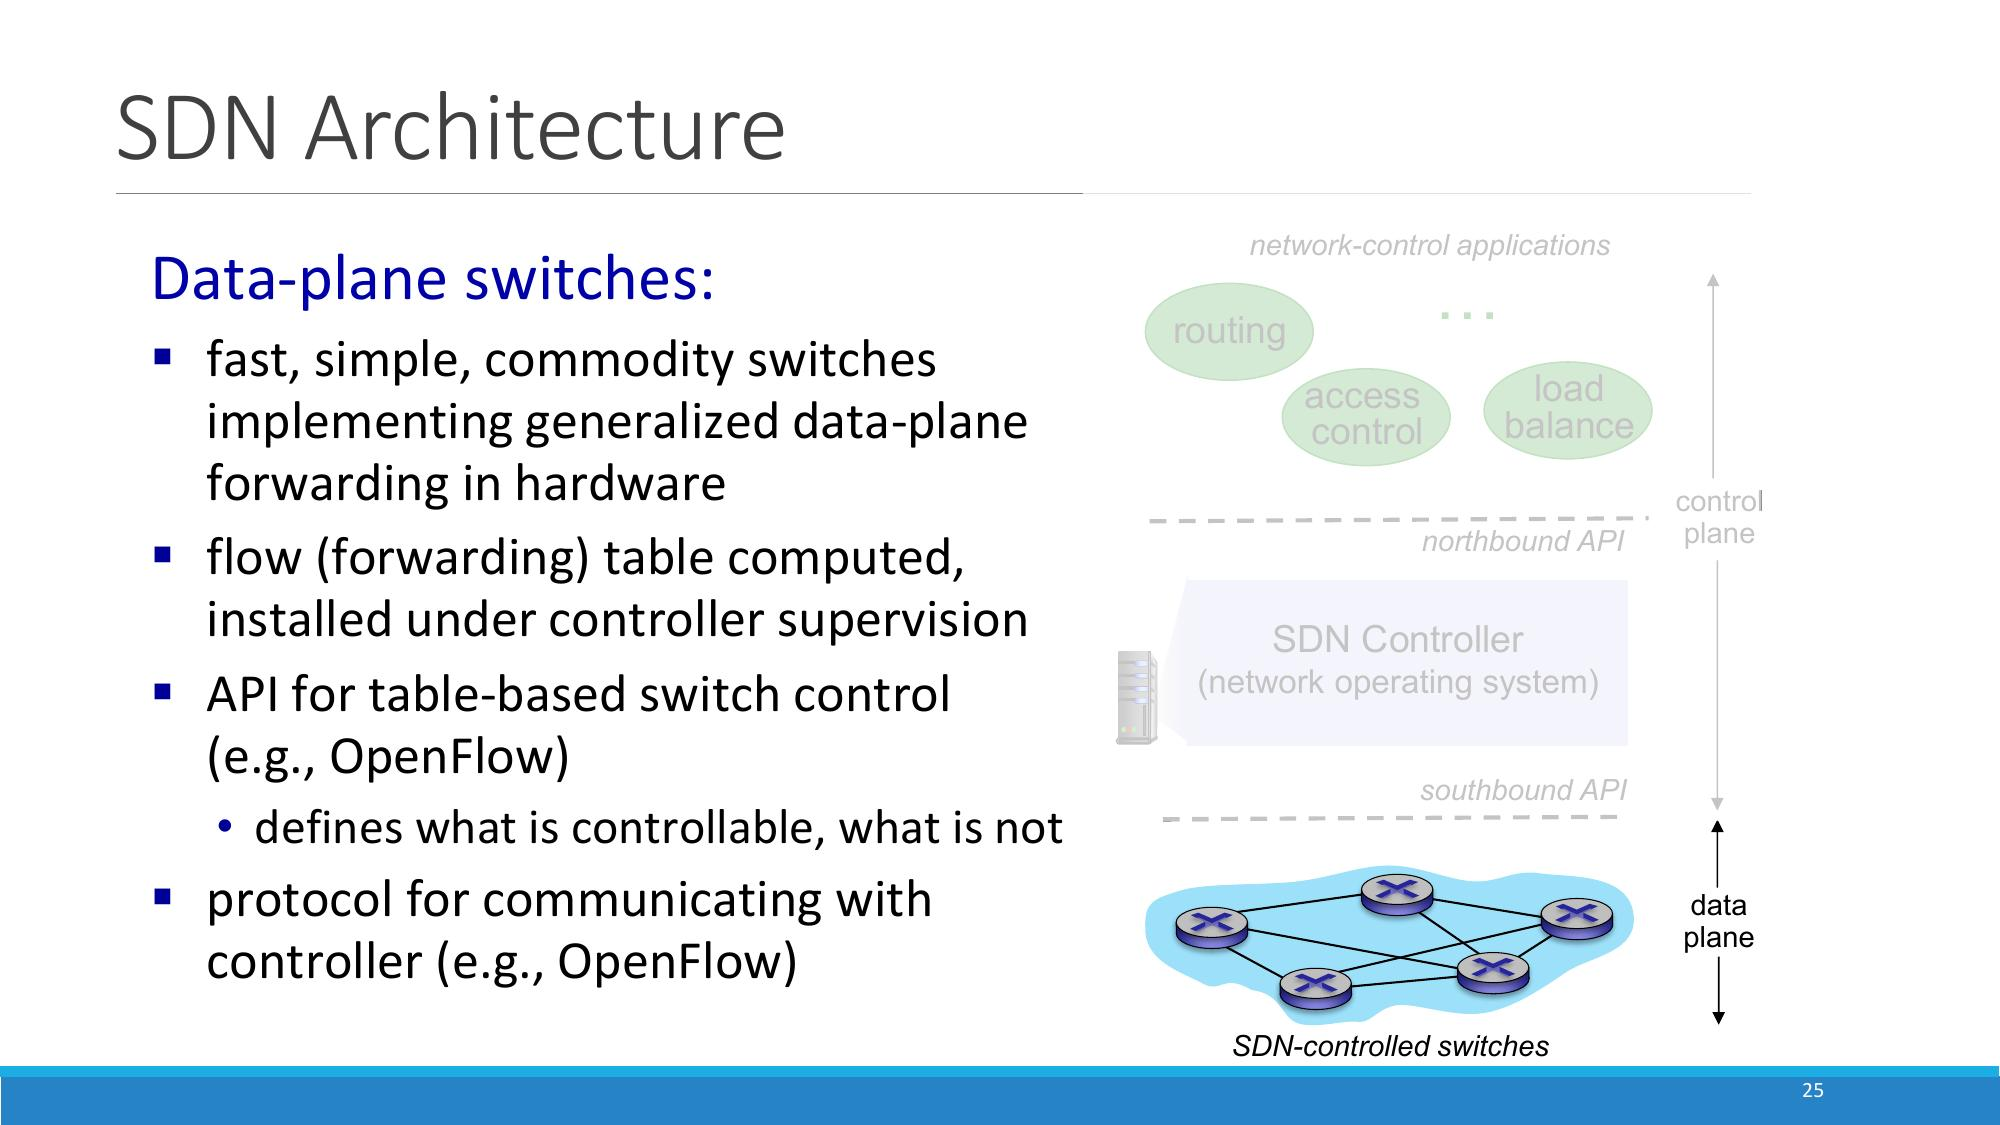
\includegraphics[keepaspectratio]{images/lezione-15-lab-sdn-architecture-img-04.jpg}}
\caption{0.3 --- L'architettura SDN è organizzata in tre livelli: le
applicazioni di controllo in cima, il controller (network OS) al centro,
e gli switch programmabili in basso. Le NorthBound API collegano
controller e applicazioni; le SouthBound API (es. OpenFlow) collegano
controller e switch.}
\end{figure}

\textbf{Data-plane switches}: switch veloci e semplici
(\emph{commodity}) che implementano il generalized forwarding in
hardware. Le flow table sono calcolate e installate sotto la
supervisione del controller. L'API per il controllo (es. OpenFlow)
definisce cosa è controllabile e cosa non lo è.

\textbf{SDN Controller} (\emph{network operating system}): mantiene le
informazioni di stato della rete, interagisce con le applicazioni via
NorthBound API e con gli switch via SouthBound API. È implementato come
sistema distribuito per performance, scalabilità, fault-tolerance e
robustezza.

\textbf{Network-control applications}: il ``cervello'' del sistema,
implementano le funzioni di controllo (routing, access control, load
balancing) usando i servizi di basso livello offerti dal controller.
Possono essere fornite da terze parti, separate dal vendor del
controller o degli switch.

\subsection{Breve Storia di SDN}\label{breve-storia-di-sdn}

{\def\LTcaptype{none} % do not increment counter
\begin{longtable}[]{@{}
  >{\raggedright\arraybackslash}p{(\linewidth - 2\tabcolsep) * \real{0.4286}}
  >{\raggedright\arraybackslash}p{(\linewidth - 2\tabcolsep) * \real{0.5714}}@{}}
\toprule\noalign{}
\begin{minipage}[b]{\linewidth}\raggedright
Anno
\end{minipage} & \begin{minipage}[b]{\linewidth}\raggedright
Evento
\end{minipage} \\
\midrule\noalign{}
\endhead
\bottomrule\noalign{}
\endlastfoot
\textasciitilde2004 & Ricerca su nuovi paradigmi di gestione (Princeton,
Stanford/Berkeley) \\
2008 & NOX Network OS (NICIRA), interfaccia OpenFlow
(Stanford/NICIRA) \\
2011 & Open Networking Foundation --- board: Google, Yahoo, Verizon;
membri: Cisco, HP, Dell \\
2013 & 1600 partecipanti all'Open Networking Summit; SDN usato nel WAN
di Google (B4) \\
2014 & SDN nei data center: VMware NSX, Cisco ACI \\
2021+ & SDN guidato da AI/ML (Cisco DNA Center, Juniper Mist AI), SDN in
reti 5G, IoT, edge; P4 per switch hardware programmabili \\
\end{longtable}
}

\begin{calloutnote}{Da protocolli distribuiti a controllo programmabile}

La traiettoria di SDN riflette una tendenza più ampia nell'informatica:
la separazione tra \emph{policy} (cosa fare) e \emph{meccanismo} (come
farlo). Così come i sistemi operativi hanno astratto l'hardware dai
programmi applicativi, SDN astrae l'infrastruttura di rete dalle
applicazioni di controllo, abilitando innovazione indipendente a ogni
livello.

\end{calloutnote}

\begin{center}\rule{0.5\linewidth}{0.5pt}\end{center}

\section{SDN Data Plane}\label{sdn-data-plane}

Il data plane, chiamato anche \emph{resource layer} o
\emph{infrastructure layer}, è composto da dispositivi di forwarding ---
switch fisici e virtuali --- che trasportano e processano i dati secondo
le decisioni del control plane. L'elemento chiave che distingue un
dispositivo SDN da un router tradizionale è l'assenza di software
autonomo per prendere decisioni di instradamento: il dispositivo esegue
soltanto le istruzioni che riceve dal controller.

\begin{figure}
\centering
\pandocbounded{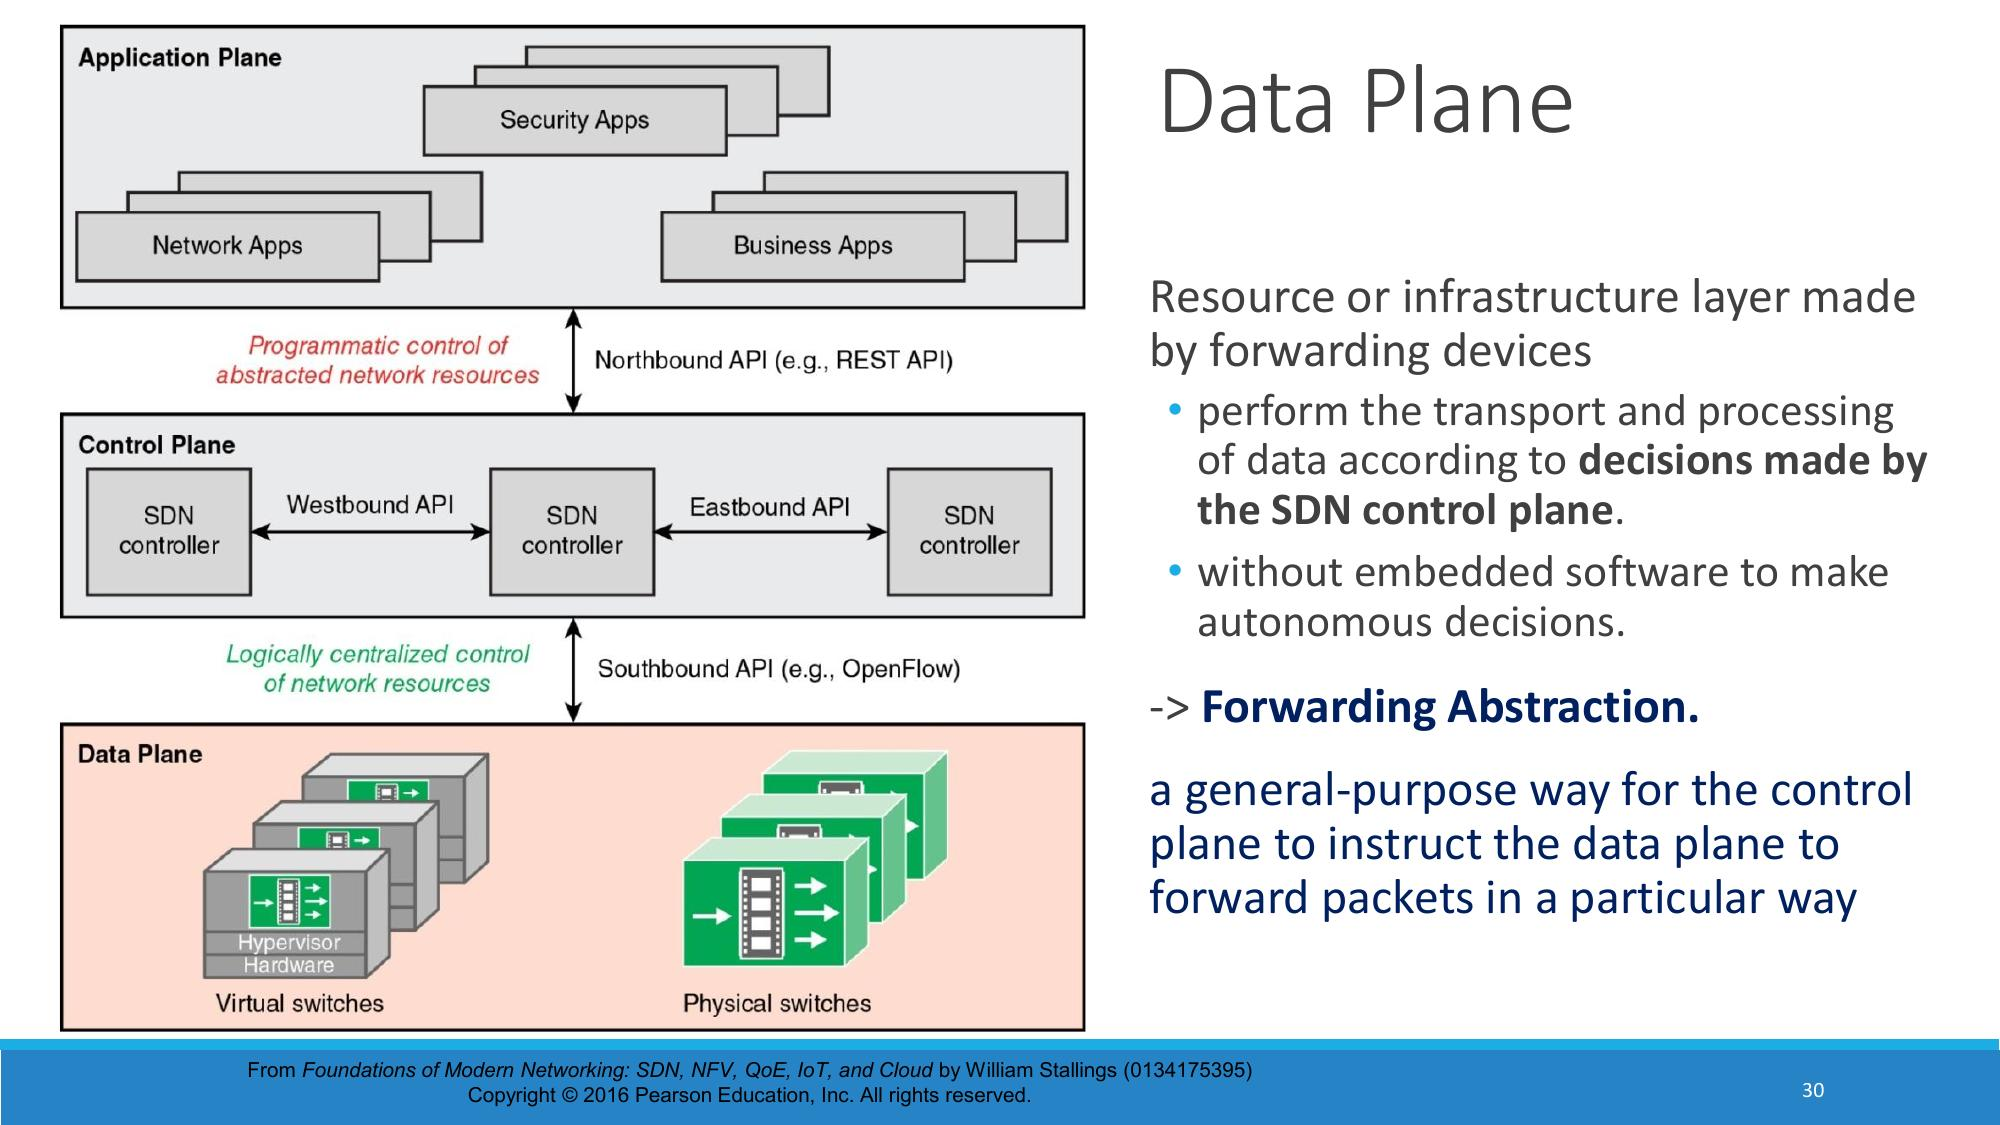
\includegraphics[keepaspectratio]{images/lezione-15-lab-sdn-architecture-img-05.jpg}}
\caption{1 --- L'architettura SDN stratificata: il Data Plane è il
livello inferiore, composto da switch che eseguono il forwarding secondo
le regole imposte dal Control Plane via SouthBound API (es. OpenFlow).}
\end{figure}

\begin{calloutdefinition}{Forwarding Abstraction}

Un meccanismo generico e standardizzato con cui il control plane
istruisce il data plane su come instradare i pacchetti. Non è legata a
un tipo specifico di dispositivo: vale tanto per router quanto per
switch o firewall.

\end{calloutdefinition}

\subsection{Forwarding Generalizzato e
Match+Action}\label{forwarding-generalizzato-e-matchaction}

Nel forwarding tradizionale basato sulla destinazione
(\emph{destination-based forwarding}), un router confronta l'indirizzo
IP di destinazione del pacchetto con la propria tabella di routing e lo
instrada di conseguenza. Il forwarding generalizzato di SDN generalizza
radicalmente questo concetto: qualsiasi campo dell'header del pacchetto
--- a livello link, rete o trasporto --- può essere usato come chiave di
corrispondenza (\emph{match}), e le azioni possibili sono molto più
ricche del semplice forwarding.

\begin{callouttip}{L’astrazione Match+Action}

Un pacchetto arriva allo switch → lo switch confronta i campi
dell'header con le voci della \textbf{flow table} → se trova
corrispondenza, esegue l'\textbf{azione} associata. Questa astrazione
unifica in un unico modello dispositivi che in passato erano separati:
router, switch, firewall, NAT.

\end{callouttip}

Le azioni possibili includono: - \textbf{drop}: scarta il pacchetto
(firewall) - \textbf{forward}: invia il pacchetto su una porta specifica
(router/switch) - \textbf{modify}: modifica campi dell'header (NAT, VLAN
rewriting) - \textbf{send to controller}: invia il pacchetto al
controller per decisione centralizzata

\subsection{Flow Table e Astrazione di
Flusso}\label{flow-table-e-astrazione-di-flusso}

Un \textbf{flusso} (\emph{flow}) è definito dall'insieme dei valori che
i campi header possono assumere. La \textbf{flow table} contiene regole
della forma:

{\def\LTcaptype{none} % do not increment counter
\begin{longtable}[]{@{}
  >{\raggedright\arraybackslash}p{(\linewidth - 2\tabcolsep) * \real{0.4800}}
  >{\raggedright\arraybackslash}p{(\linewidth - 2\tabcolsep) * \real{0.5200}}@{}}
\toprule\noalign{}
\begin{minipage}[b]{\linewidth}\raggedright
Componente
\end{minipage} & \begin{minipage}[b]{\linewidth}\raggedright
Descrizione
\end{minipage} \\
\midrule\noalign{}
\endhead
\bottomrule\noalign{}
\endlastfoot
\textbf{Match} & Pattern da confrontare con i campi header (wildcard
\texttt{*} per qualsiasi valore) \\
\textbf{Action} & Cosa fare con il pacchetto che corrisponde \\
\textbf{Priority} & Priorità per risolvere ambiguità tra regole
sovrapposte \\
\textbf{Counters} & Contatori di byte e pacchetti per statistica \\
\end{longtable}
}

I campi su cui si può effettuare il match coprono tre livelli OSI
contemporaneamente: porta di ingresso, MAC sorgente/destinazione, tipo
Ethernet, VLAN ID, IP sorgente/destinazione, protocollo IP, ToS, porte
TCP/UDP sorgente e destinazione. Questa flessibilità consente di
implementare policy di rete complesse con un singolo meccanismo
uniforme.

\begin{callouttip}{Esempi di regole OpenFlow}

\begin{itemize}
\tightlist
\item
  \textbf{Forwarding IP classico}: \texttt{IP\ Dst\ =\ 51.6.0.8} →
  \texttt{forward(port\ 6)} --- tutti i datagrammi verso quell'IP
  vengono instradati sulla porta 6.
\item
  \textbf{Firewall (blocca SSH)}: \texttt{TCP\ dst-port\ =\ 22} →
  \texttt{drop} --- blocca tutti i pacchetti TCP destinati alla porta
  22.
\item
  \textbf{Blocco per sorgente}: \texttt{IP\ Src\ =\ 128.119.1.1} →
  \texttt{drop} --- blocca tutto il traffico da quell'host.
\item
  \textbf{L2 forwarding}: \texttt{Eth\ Dst\ =\ 22:A7:23:11:E1:02} →
  \texttt{forward(port\ 3)} --- forwarding basato su MAC address.
\end{itemize}

\end{callouttip}

\begin{center}\rule{0.5\linewidth}{0.5pt}\end{center}

\subsection{OpenFlow}\label{openflow}

\textbf{OpenFlow} è il protocollo standard che implementa la
\emph{SouthBound API} di SDN. Definisce come il controller comunica con
i dispositivi di forwarding per installare, modificare e rimuovere
regole nella flow table. Il primo paper che lo ha introdotto è di Nick
McKeown et al.~(2008) e ha dato origine a un intero ecosistema gestito
oggi dalla \emph{Open Networking Foundation (ONF)}.

\begin{calloutdefinition}{OpenFlow}

Protocollo di comunicazione nelle architetture SDN che permette ai
controller di consegnare \emph{forwarding entries} ai dispositivi di
data plane (switch e router, fisici e virtuali). È la principale
implementazione della SouthBound API.

\end{calloutdefinition}

Sebbene l'adozione in ambienti di produzione rimanga limitata, OpenFlow
ha un valore fondamentale per la ricerca e la didattica, avendo ispirato
soluzioni più avanzate come \textbf{P4} (p4.org) per la programmazione
generalizzata del data plane.

\subsubsection{Struttura di una Flow Entry
OpenFlow}\label{struttura-di-una-flow-entry-openflow}

Ogni voce nella flow table OpenFlow ha tre campi fondamentali:

\begin{enumerate}
\def\labelenumi{\arabic{enumi}.}
\tightlist
\item
  \textbf{Match}: i campi header da confrontare (tutti i livelli)
\item
  \textbf{Action}: le operazioni da eseguire (forward, drop, modify
  header, encapsulate e invia al controller)
\item
  \textbf{Stats}: contatori di pacchetti e byte per monitoraggio
\end{enumerate}

\subsubsection{OpenFlow come Astrazione
Unificante}\label{openflow-come-astrazione-unificante}

\begin{callouttip}{Un solo modello per tutti i dispositivi}

{\def\LTcaptype{none} % do not increment counter
\begin{longtable}[]{@{}lll@{}}
\toprule\noalign{}
Dispositivo & Match & Action \\
\midrule\noalign{}
\endhead
\bottomrule\noalign{}
\endlastfoot
Router & Longest prefix IP dst & Forward su link \\
Switch L2 & MAC address destinazione & Forward o flood \\
Firewall & IP + TCP/UDP port & Permit o deny \\
NAT & IP address e port & Rewrite address e port \\
\end{longtable}
}

Tutti questi dispositivi, storicamente separati, diventano istanze della
stessa astrazione match+action con flow table diverse.

\end{callouttip}

\begin{center}\rule{0.5\linewidth}{0.5pt}\end{center}

\subsection{OpenFlow Switch e Flow Table
Pipeline}\label{openflow-switch-e-flow-table-pipeline}

Un OpenFlow switch ha tre componenti principali:

\begin{enumerate}
\def\labelenumi{\arabic{enumi}.}
\tightlist
\item
  \textbf{Porte I/O}: le interfacce fisiche attraverso cui entrano ed
  escono i pacchetti
\item
  \textbf{Flow Tables} (\emph{Datapath}): tabelle organizzate in
  pipeline per il processing dei pacchetti
\item
  \textbf{OpenFlow Channel}: il canale di comunicazione sicuro (TCP,
  opzionalmente TLS) con il controller
\end{enumerate}

\begin{figure}
\centering
\pandocbounded{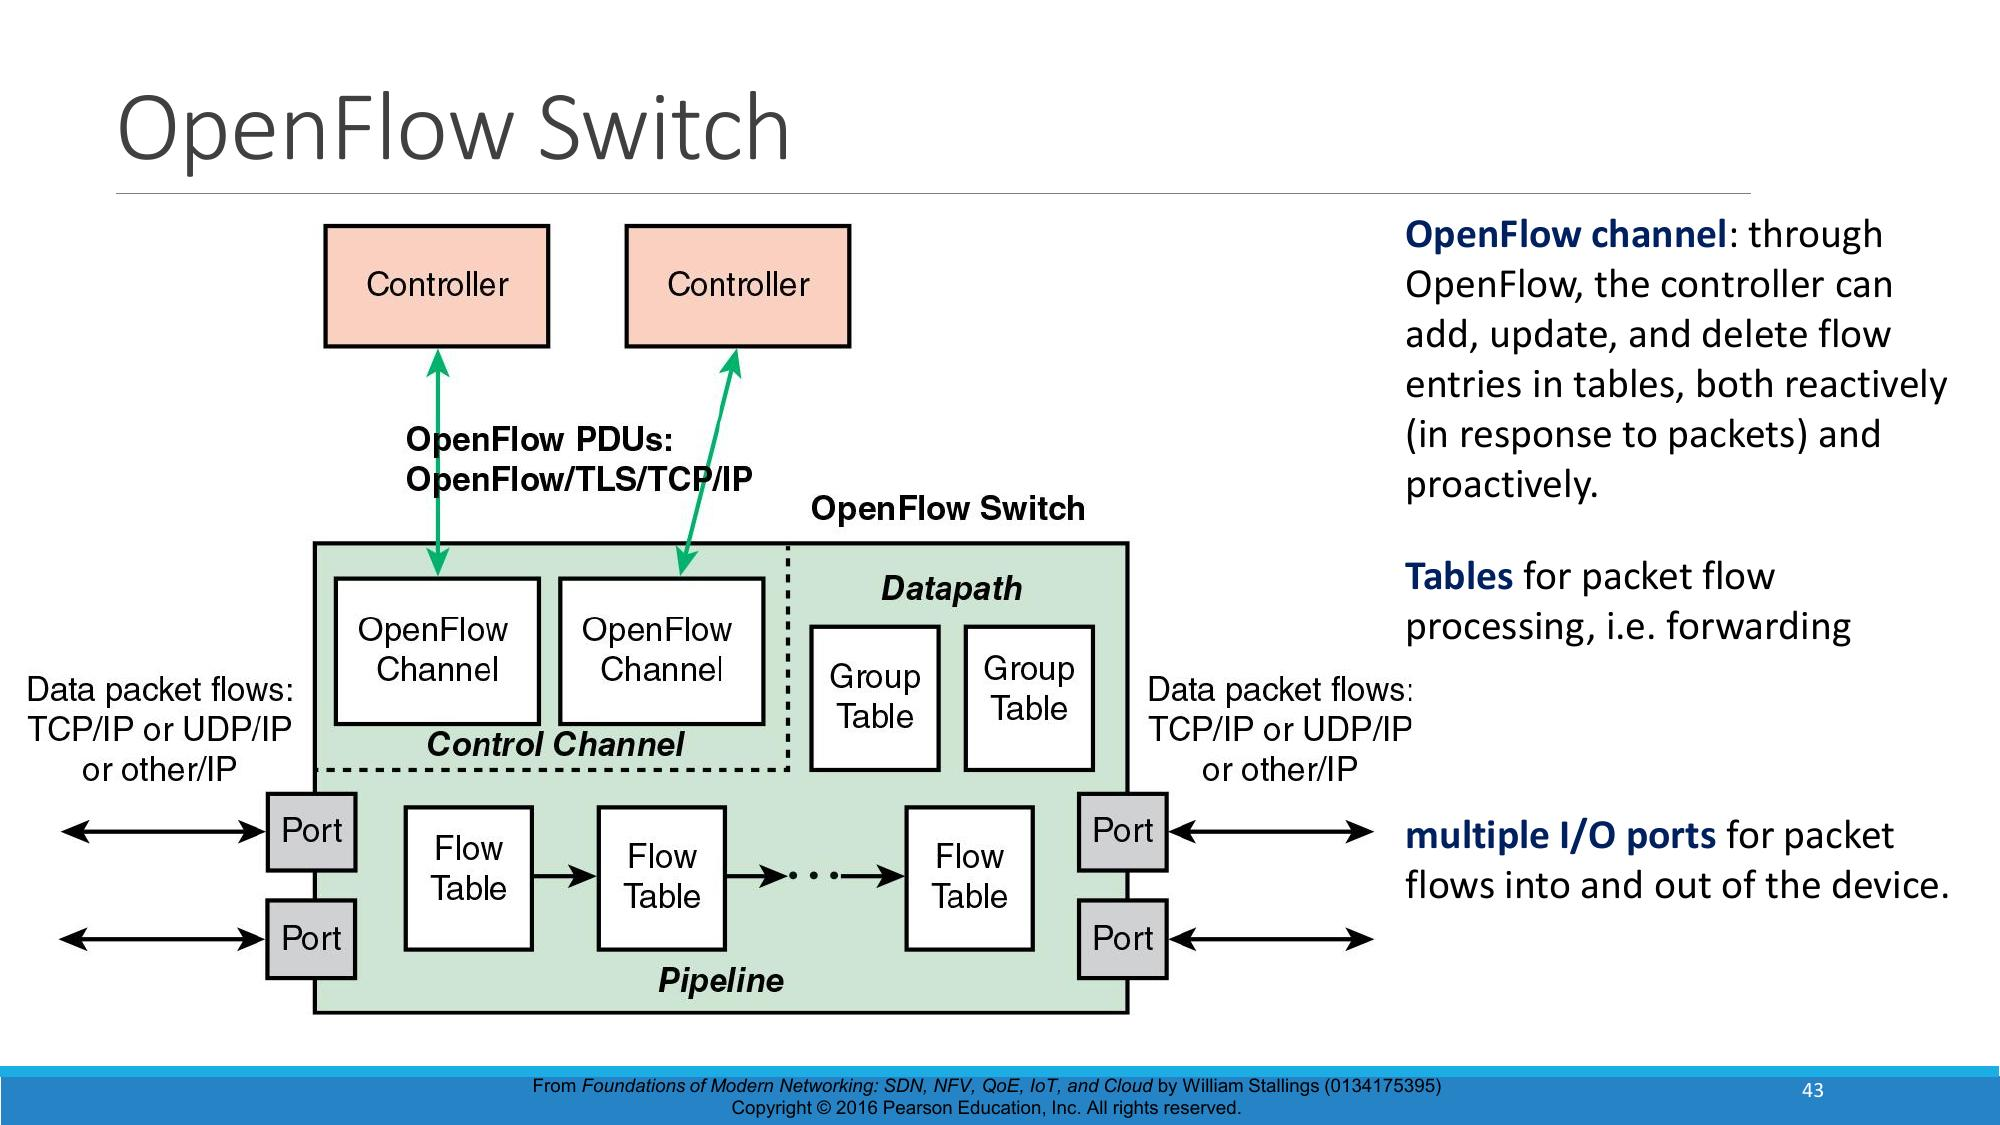
\includegraphics[keepaspectratio]{images/lezione-15-lab-sdn-architecture-img-06.jpg}}
\caption{2 --- L'OpenFlow Switch: il canale OpenFlow collega lo switch
al controller, che può aggiungere, aggiornare e rimuovere flow entries
sia in modo reattivo (in risposta ai pacchetti) che proattivo.}
\end{figure}

\subsubsection{Flow Table Pipeline}\label{flow-table-pipeline}

Uno switch può contenere \textbf{una o più flow table} organizzate in
\textbf{pipeline}. Le tabelle sono numerate sequenzialmente a partire da
0. Il pacchetto viene processato prima dalla tabella 0, e in base al
risultato del match può essere diretto ad altre tabelle, a una group
table, a una meter table, o infine all'uscita.

\[
\text{Packet in} \rightarrow [\text{Table 0}] \rightarrow [\text{Table 1}] \rightarrow \cdots \rightarrow [\text{Table N}] \rightarrow \text{Packet out}
\]

L'uso di più tabelle in pipeline offre al controller notevole
flessibilità: permette, ad esempio, di separare le regole di sicurezza
da quelle di routing in tabelle distinte, applicandole in sequenza.

\subsubsection{Processing Pipeline}\label{processing-pipeline}

Quando un pacchetto viene processato da una flow table: - Se c'è
\textbf{corrispondenza} con una o più entry, viene eseguita la regola
con \textbf{priorità più alta}. Le istruzioni possono aggiornare
l'action set, aggiornare metadata, eseguire azioni, o redirigere il
pacchetto con \texttt{Goto} a un'altra tabella. - Se c'è corrispondenza
solo con la \textbf{table-miss entry} (entry speciale per pacchetti
senza match), si può: (a) inviare al controller, (b) redirigere a
un'altra tabella, (c) scartare. - Se \textbf{non c'è alcun match} e non
esiste table-miss entry, il pacchetto viene \textbf{scartato}.

\begin{center}\rule{0.5\linewidth}{0.5pt}\end{center}

\subsection{Group Tables}\label{group-tables}

Oltre alle flow table, OpenFlow definisce le \textbf{group table}. Un
pacchetto che corrisponde a una flow entry può essere diretto non a una
singola porta di uscita, ma a un \emph{group entry}, che specifica come
il pacchetto deve essere gestito su più porte.

Ogni group entry ha: - Un \textbf{Group ID} univoco - Un \textbf{Group
Type} che definisce la semantica - Uno o più \textbf{action bucket} con
le azioni possibili

{\def\LTcaptype{none} % do not increment counter
\begin{longtable}[]{@{}
  >{\raggedright\arraybackslash}p{(\linewidth - 2\tabcolsep) * \real{0.4615}}
  >{\raggedright\arraybackslash}p{(\linewidth - 2\tabcolsep) * \real{0.5385}}@{}}
\toprule\noalign{}
\begin{minipage}[b]{\linewidth}\raggedright
Group Type
\end{minipage} & \begin{minipage}[b]{\linewidth}\raggedright
Comportamento
\end{minipage} \\
\midrule\noalign{}
\endhead
\bottomrule\noalign{}
\endlastfoot
\textbf{ALL} & Il pacchetto viene inviato a tutti i bucket
(multicast/broadcast) \\
\textbf{SELECT} & Il pacchetto viene inviato a un singolo bucket scelto
per load balancing o hashing \\
\end{longtable}
}

\begin{callouttip}{Group Table in azione}

\begin{itemize}
\tightlist
\item
  Group 1 (ALL): Output su Port 2 e Port 3 → flooding su entrambe le
  porte
\item
  Group 2 (SELECT): Output su Port 4 o Port 5 → bilanciamento del carico
  tra due link
\end{itemize}

\end{callouttip}

\begin{center}\rule{0.5\linewidth}{0.5pt}\end{center}

\section{SDN Control Plane}\label{sdn-control-plane}

Il control plane SDN è il livello di intelligenza della rete.
Centralizza la logica di instradamento, il calcolo dei percorsi e la
gestione delle policy in un componente software chiamato
\textbf{controller SDN}, che mantiene una visione globale e consistente
dello stato della rete.

\subsection{Componenti del Controller
SDN}\label{componenti-del-controller-sdn}

Il controller SDN è organizzato in tre strati funzionali:

\textbf{Strato di comunicazione (\emph{Communication Layer})}: gestisce
la comunicazione bidirezionale tra il controller e i dispositivi del
data plane. I protocolli utilizzati sono OpenFlow (SouthBound API),
SNMP, e altri.

\textbf{Strato di gestione dello stato di rete (\emph{Network-Wide State
Management})}: mantiene un database distribuito con le informazioni
sullo stato dell'intera rete: topologia dei link, informazioni sugli
host, flow table degli switch, statistiche. È il cuore del controller,
poiché fornisce la \emph{global network view} necessaria per decisioni
di routing ottimali.

\textbf{Strato di interfaccia verso le applicazioni (\emph{Interface
Layer})}: espone API (\emph{NorthBound API}) alle applicazioni di
controllo (routing, access control, load balancing, orchestrazione).
Queste API permettono alle applicazioni di interagire con la rete in
modo astratto, senza conoscere i dettagli del protocollo SouthBound.

\subsection{Protocollo OpenFlow ---
Messaggi}\label{protocollo-openflow-messaggi}

OpenFlow opera tra controller e switch tramite \textbf{TCP}
(opzionalmente cifrato con TLS). I messaggi sono divisi in tre classi:

\textbf{Controller → Switch:}

{\def\LTcaptype{none} % do not increment counter
\begin{longtable}[]{@{}
  >{\raggedright\arraybackslash}p{(\linewidth - 2\tabcolsep) * \real{0.5238}}
  >{\raggedright\arraybackslash}p{(\linewidth - 2\tabcolsep) * \real{0.4762}}@{}}
\toprule\noalign{}
\begin{minipage}[b]{\linewidth}\raggedright
Messaggio
\end{minipage} & \begin{minipage}[b]{\linewidth}\raggedright
Funzione
\end{minipage} \\
\midrule\noalign{}
\endhead
\bottomrule\noalign{}
\endlastfoot
\textbf{features} & Il controller interroga lo switch sulle sue
capacità, lo switch risponde \\
\textbf{configure} & Il controller legge o imposta parametri di
configurazione dello switch \\
\textbf{modify-state (FlowMod)} & Aggiunge, elimina o modifica flow
entries nelle tabelle OpenFlow \\
\textbf{packet-out} & Il controller invia un pacchetto incapsulato a una
porta specifica dello switch \\
\end{longtable}
}

\textbf{Switch → Controller:}

{\def\LTcaptype{none} % do not increment counter
\begin{longtable}[]{@{}
  >{\raggedright\arraybackslash}p{(\linewidth - 2\tabcolsep) * \real{0.5238}}
  >{\raggedright\arraybackslash}p{(\linewidth - 2\tabcolsep) * \real{0.4762}}@{}}
\toprule\noalign{}
\begin{minipage}[b]{\linewidth}\raggedright
Messaggio
\end{minipage} & \begin{minipage}[b]{\linewidth}\raggedright
Funzione
\end{minipage} \\
\midrule\noalign{}
\endhead
\bottomrule\noalign{}
\endlastfoot
\textbf{packet-in} & Lo switch trasferisce un pacchetto (e il suo
controllo) al controller \\
\textbf{flow-removed} & Notifica che una flow entry è stata eliminata
dallo switch \\
\textbf{port-status} & Informa il controller di un cambiamento di stato
su una porta \\
\end{longtable}
}

\begin{calloutwarning}{I network operator non programmano OpenFlow direttamente}

In pratica, gli operatori usano astrazioni di alto livello fornite dal
controller (es. intent framework in ONOS). La scrittura diretta di
messaggi OpenFlow è riservata allo sviluppo interno del controller.

\end{calloutwarning}

\subsection{Interazione Control Plane / Data Plane ---
Esempio}\label{interazione-control-plane-data-plane-esempio}

Un esempio concreto illustra la collaborazione tra i componenti. Si
consideri un guasto su un link della rete:

\begin{enumerate}
\def\labelenumi{\arabic{enumi}.}
\tightlist
\item
  Lo switch \textbf{S1} rileva il guasto e invia al controller un
  messaggio \textbf{port-status} per notificare il cambiamento di stato
  del link.
\item
  Il \textbf{controller SDN} riceve il messaggio e aggiorna il proprio
  database di stato dei link.
\item
  L'applicazione di routing \textbf{Dijkstra} (che si è registrata per
  ricevere notifiche sui cambiamenti di link) viene invocata.
\item
  Dijkstra accede al grafo della rete e alle informazioni di link-state
  nel controller e calcola i \textbf{nuovi percorsi ottimali}.
\item
  L'applicazione di routing interagisce con il componente di calcolo
  delle flow table nel controller per determinare le nuove regole da
  installare.
\item
  Il controller invia messaggi \textbf{FlowMod} via OpenFlow agli switch
  interessati per installare le nuove flow table.
\end{enumerate}

\begin{calloutnote}{SDN vs routing distribuito tradizionale}

In una rete tradizionale, i router eseguono OSPF o BGP e calcolano i
percorsi autonomamente scambiandosi informazioni. In SDN, questa logica
è centralizzata nel controller: questo semplifica il coordinamento, ma
richiede robustezza e alta disponibilità del controller stesso.

\end{calloutnote}

\begin{center}\rule{0.5\linewidth}{0.5pt}\end{center}

\subsection{Implementazioni di Controller
SDN}\label{implementazioni-di-controller-sdn}

{\def\LTcaptype{none} % do not increment counter
\begin{longtable}[]{@{}
  >{\raggedright\arraybackslash}p{(\linewidth - 2\tabcolsep) * \real{0.6667}}
  >{\raggedright\arraybackslash}p{(\linewidth - 2\tabcolsep) * \real{0.3333}}@{}}
\toprule\noalign{}
\begin{minipage}[b]{\linewidth}\raggedright
Controller
\end{minipage} & \begin{minipage}[b]{\linewidth}\raggedright
Note
\end{minipage} \\
\midrule\noalign{}
\endhead
\bottomrule\noalign{}
\endlastfoot
\textbf{NOX} & Primo controller SDN, riferimento storico \\
\textbf{Ryu} & Framework Python per SDN \\
\textbf{OpenDaylight (ODL)} & Controller open source enterprise-grade \\
\textbf{ONOS} & Open Network OS, forte enfasi su distribuzione e
scalabilità \\
\textbf{TeraFlow SDN} & Controller per reti cloud-native, progetto
ETSI \\
\end{longtable}
}

\subsubsection{OpenDaylight (ODL)}\label{opendaylight-odl}

OpenDaylight è uno dei controller SDN più diffusi in ambienti
enterprise. La sua architettura è stratificata:

\begin{itemize}
\tightlist
\item
  \textbf{Northbound API}: REST/RESTCONF/NETCONF per le applicazioni
  (Traffic Engineering, Firewalling, Load Balancing, Orchestration)
\item
  \textbf{Basic Network Functions}: moduli interni per topology
  processing, switch management, statistiche, host tracking, gestione
  regole di forwarding
\item
  \textbf{Service Abstraction Layer (SAL)}: il bus interno che
  interconnette applicazioni, servizi interni e protocolli SouthBound
\item
  \textbf{Southbound API}: OpenFlow, NETCONF, SNMP, OVSDB
\end{itemize}

\begin{callouttip}{SAL in ODL}

Il Service Abstraction Layer è l'elemento architetturale chiave di ODL:
agisce da mediatore tra il mondo delle applicazioni (Northbound) e i
protocolli di rete specifici (Southbound), rendendo il controller
agnostico rispetto al protocollo SouthBound utilizzato.

\end{callouttip}

\subsubsection{ONOS}\label{onos}

ONOS (\emph{Open Network Operating System}) enfatizza la separazione
delle applicazioni di controllo dal core del controller e la robustezza
distribuita:

\begin{itemize}
\tightlist
\item
  Le \textbf{applicazioni di controllo} (Traffic Engineering,
  Firewalling, Load Balancing) sono separate dal controller core e
  comunicano via Northbound API
\item
  L'\textbf{intent framework} permette alle applicazioni di specificare
  \emph{cosa} si vuole ottenere (es. connettività tra due host)
  piuttosto che \emph{come} (es. quale percorso usare): il controller si
  occupa di tradurre l'intent in flow rules concrete
\item
  Il \textbf{distributed core} garantisce alta disponibilità e
  scalabilità attraverso replicazione e consensus distribuito
\end{itemize}

\begin{center}\rule{0.5\linewidth}{0.5pt}\end{center}

\section{Forwarding e Topology
Discovery}\label{forwarding-e-topology-discovery}

Un aspetto cruciale in una rete SDN è come il controller costruisce la
conoscenza della topologia e come gestisce il forwarding dei pacchetti
prima che le flow table siano popolate.

\subsection{Path Computation}\label{path-computation}

\begin{figure}
\centering
\pandocbounded{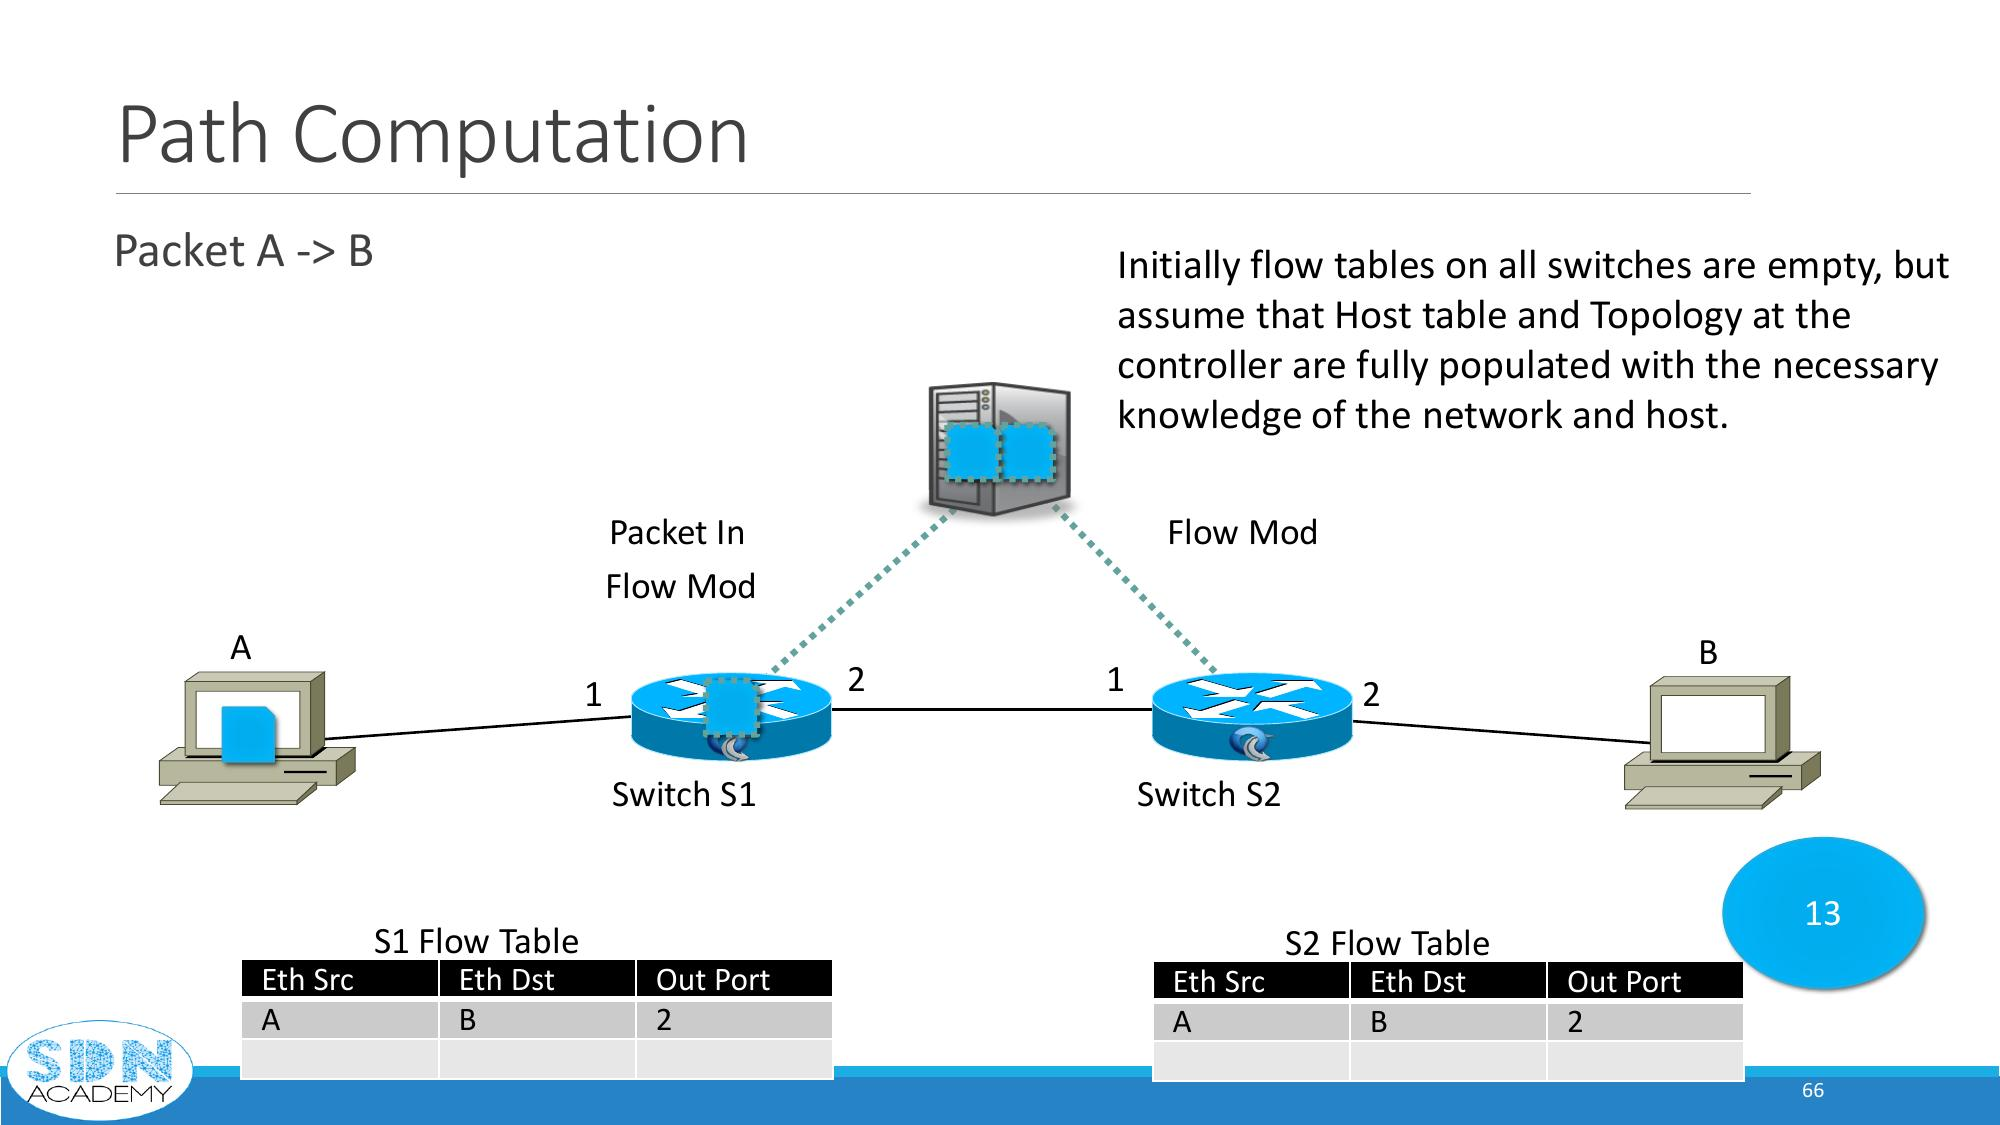
\includegraphics[keepaspectratio]{images/lezione-15-lab-sdn-architecture-img-07.jpg}}
\caption{3 --- Path computation: le flow table degli switch sono
inizialmente vuote. Il primo pacchetto da A a B genera un Packet-In; il
controller calcola il percorso e installa le regole via FlowMod.}
\end{figure}

Quando un pacchetto arriva a uno switch e non trova corrispondenza nella
flow table (\emph{table-miss}), lo switch lo invia al controller tramite
un messaggio \textbf{Packet-In}. Il controller, disponendo di una Host
Table e di una Topology Table già popolate, calcola il percorso ottimale
da sorgente a destinazione e invia messaggi \textbf{FlowMod} agli switch
lungo il percorso.

\begin{calloutwarning}{Ordine di installazione delle flow entries}

I messaggi FlowMod vengono inviati in \textbf{ordine inverso}: prima
allo switch più vicino alla destinazione, poi risalendo verso la
sorgente. Questo garantisce che quando il pacchetto arriva al secondo
switch, la regola sia già installata, evitando un secondo Packet-In al
controller.

\end{calloutwarning}

Una volta installate le regole, tutti i pacchetti successivi dello
stesso flusso vengono gestiti direttamente dagli switch, senza passare
dal controller.

\begin{center}\rule{0.5\linewidth}{0.5pt}\end{center}

\subsection{Routing Centralizzato}\label{routing-centralizzato}

In una rete tradizionale, la funzione di routing è distribuita tra i
router, ognuno dei quali mantiene la propria tabella di routing e
partecipa a protocolli come OSPF. In SDN, è naturale centralizzare
questa funzione nel controller, che:

\begin{itemize}
\tightlist
\item
  Ha una visione \textbf{globale e coerente} dello stato della rete
\item
  Può implementare \textbf{policy application-aware} (es. preferire
  certi link per certi tipi di traffico)
\item
  Libera gli switch dal burden computazionale e di storage del routing,
  migliorandone le prestazioni
\end{itemize}

Il routing centralizzato svolge due funzioni distinte:

\begin{enumerate}
\def\labelenumi{\arabic{enumi}.}
\tightlist
\item
  \textbf{Link/Topology Discovery}: il controller deve conoscere i link
  tra gli switch del data plane (non standardizzata in OpenFlow, ogni
  implementazione ha il proprio approccio)
\item
  \textbf{Topology Manager}: mantiene la topologia aggiornata e calcola
  i percorsi più brevi tra nodi
\end{enumerate}

\begin{center}\rule{0.5\linewidth}{0.5pt}\end{center}

\subsection{Inizializzazione degli
Switch}\label{inizializzazione-degli-switch}

\begin{figure}
\centering
\pandocbounded{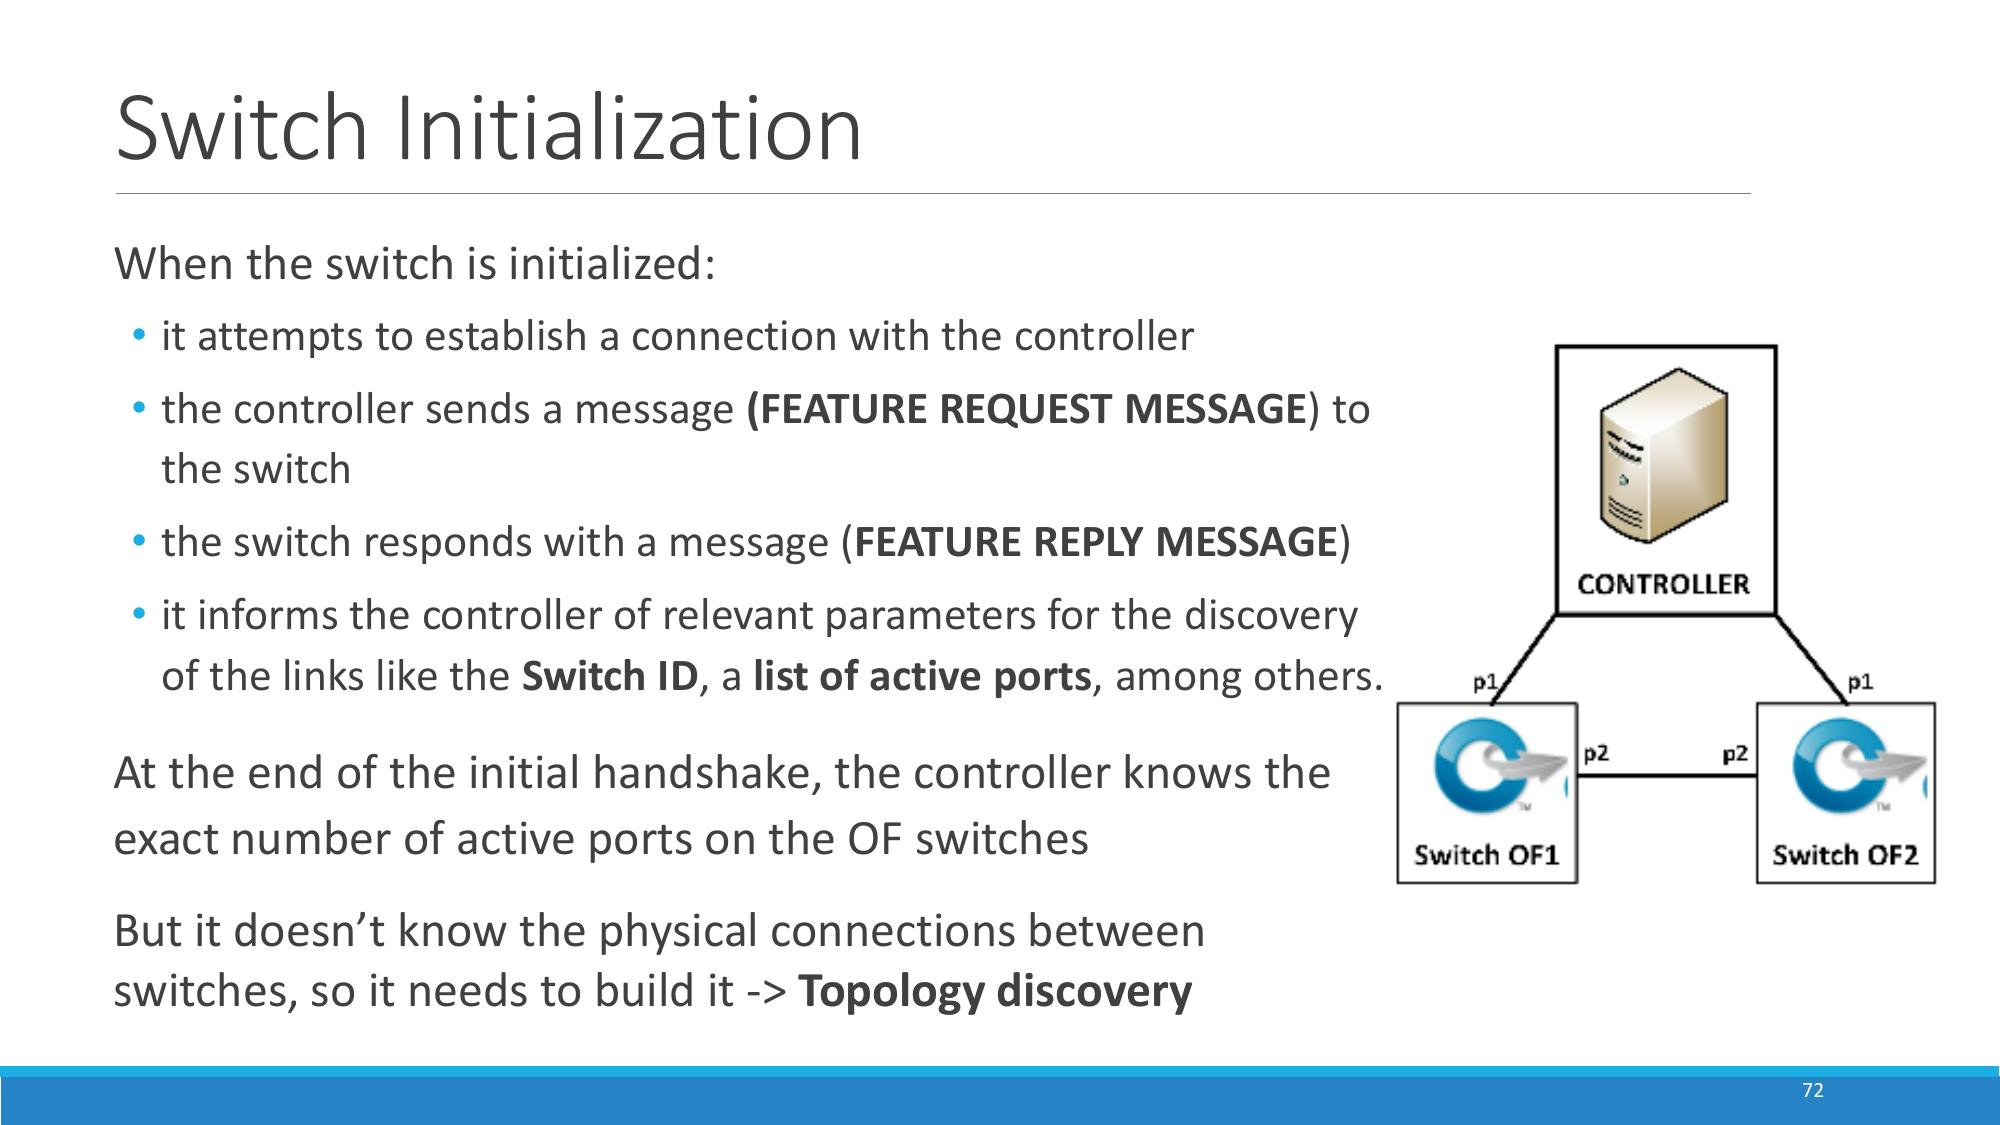
\includegraphics[keepaspectratio]{images/lezione-15-lab-sdn-architecture-img-08.jpg}}
\caption{4 --- Switch Initialization: al boot, lo switch stabilisce una
connessione TCP con il controller. Lo scambio Feature Request / Feature
Reply comunica al controller i parametri dello switch (Switch ID, porte
attive).}
\end{figure}

Quando uno switch OpenFlow viene acceso, esegue una procedura di
handshake con il controller:

\begin{enumerate}
\def\labelenumi{\arabic{enumi}.}
\tightlist
\item
  Lo switch tenta di stabilire una \textbf{connessione TCP} con
  l'indirizzo del controller (pre-configurato)
\item
  Il controller invia un messaggio \textbf{FEATURE REQUEST}
\item
  Lo switch risponde con un messaggio \textbf{FEATURE REPLY} contenente:
  Switch ID, lista delle porte attive, e altri parametri rilevanti
\end{enumerate}

Al termine dell'handshake, il controller sa esattamente quante porte
attive ha ogni switch, ma \textbf{non conosce ancora le connessioni
fisiche tra switch}. Per questo è necessaria la topology discovery.

\begin{center}\rule{0.5\linewidth}{0.5pt}\end{center}

\subsection{Topology Discovery con
LLDP}\label{topology-discovery-con-lldp}

La topology discovery in reti OpenFlow si basa sul \textbf{Link Layer
Discovery Protocol (LLDP)}, standardizzato da IEEE nel 2005 e 2009. LLDP
è un protocollo \emph{vendor-neutral} che opera al Livello 2 del modello
OSI e permette a un dispositivo di annunciare la propria identità e le
proprie capacità ai dispositivi adiacenti.

Gli switch OpenFlow hanno due configurazioni iniziali che abilitano la
topology discovery: 1. \textbf{Indirizzo del controller}: ogni switch ha
pre-configurato l'IP e la porta TCP del controller, a cui si connette al
boot 2. \textbf{Flow rule per LLDP}: ogni switch ha una regola
pre-installata che invia al controller (via Packet-In) qualsiasi frame
LLDP ricevuto

\subsubsection{Struttura del Frame LLDP}\label{struttura-del-frame-lldp}

\begin{figure}
\centering
\pandocbounded{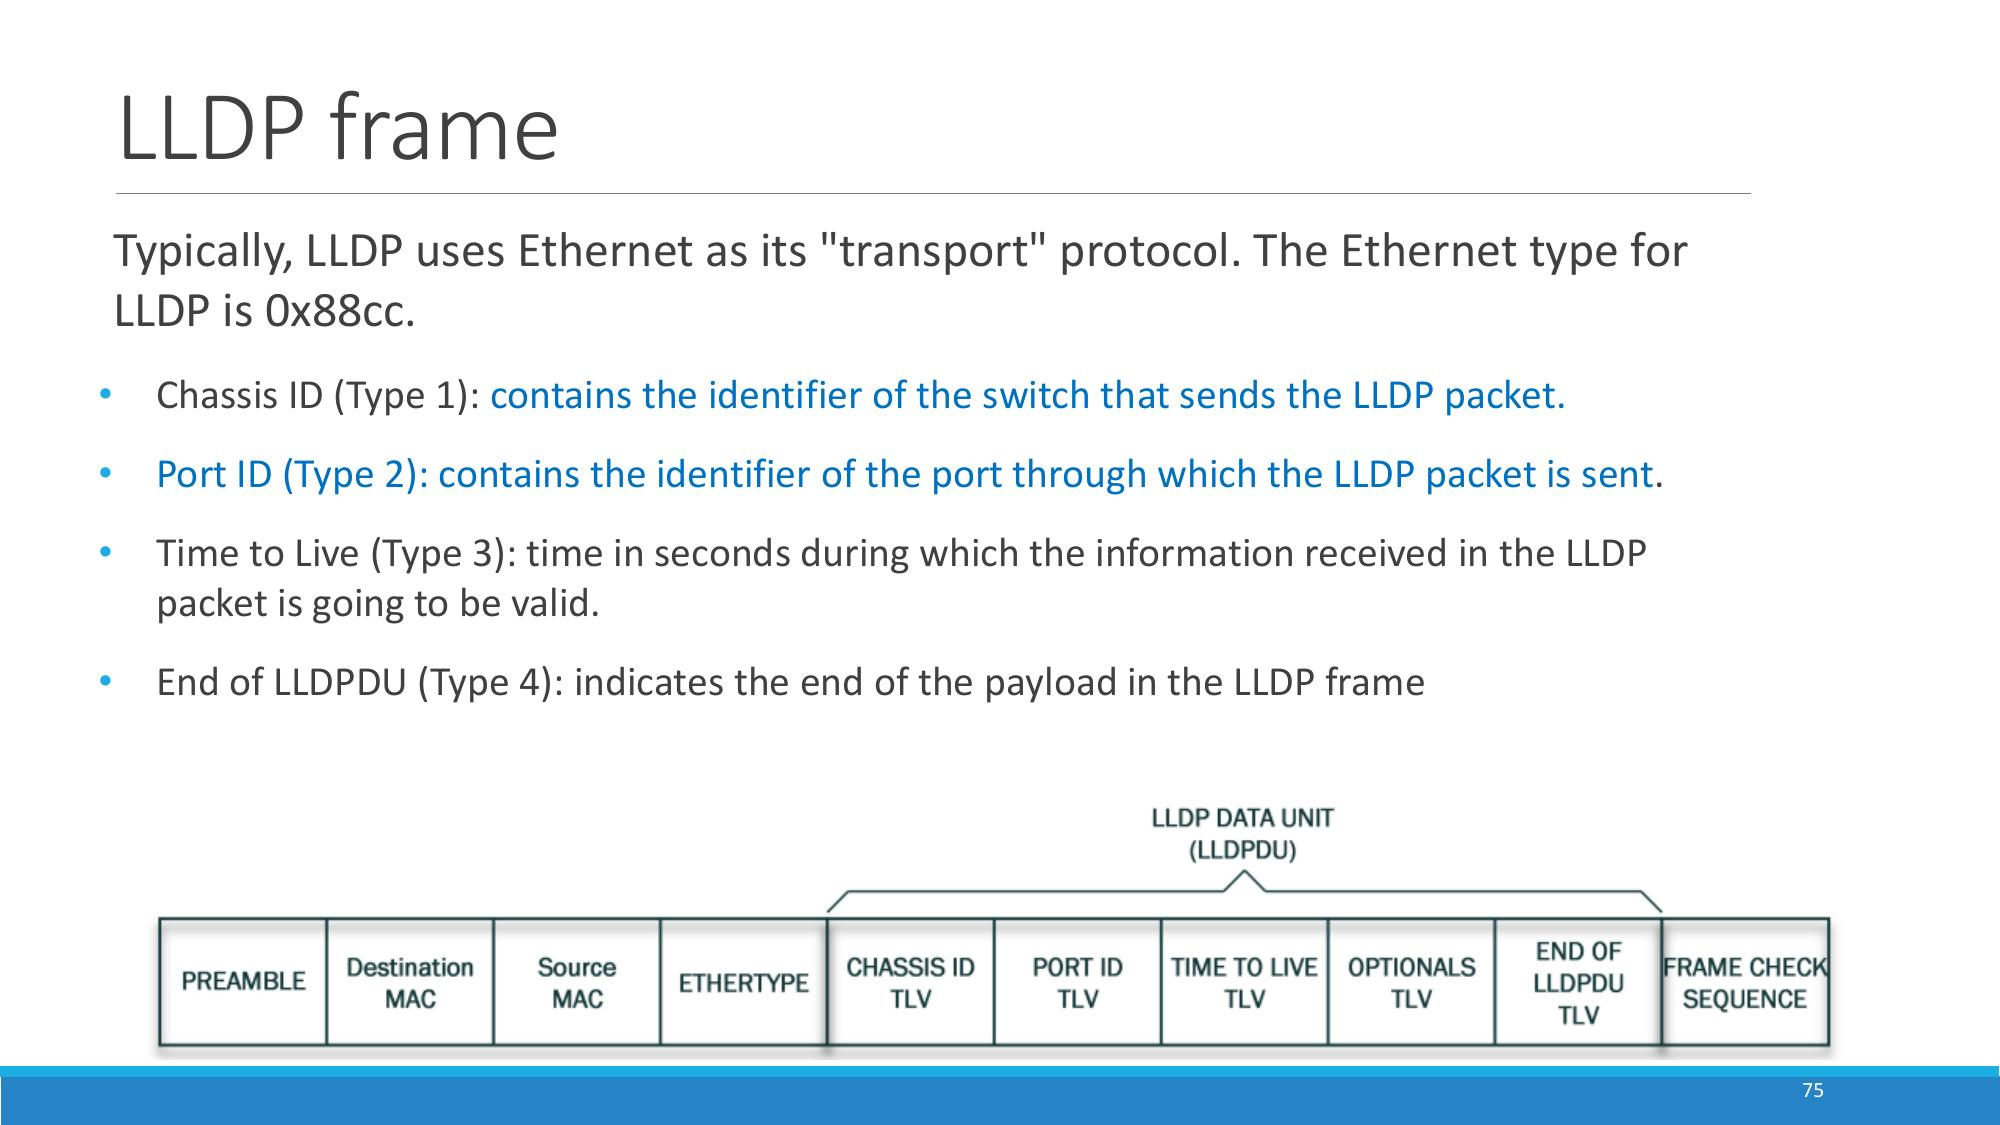
\includegraphics[keepaspectratio]{images/lezione-15-lab-sdn-architecture-img-09.jpg}}
\caption{5 --- Struttura del frame LLDP. Il tipo Ethernet è 0x88cc. I
TLV (Type-Length-Value) fondamentali sono: Chassis ID (switch mittente),
Port ID (porta mittente), TTL, End of LLDPDU.}
\end{figure}

Il frame LLDP usa Ethernet come protocollo di trasporto (EtherType
\texttt{0x88cc}) e contiene i seguenti campi TLV
(\emph{Type-Length-Value}):

{\def\LTcaptype{none} % do not increment counter
\begin{longtable}[]{@{}
  >{\raggedright\arraybackslash}p{(\linewidth - 4\tabcolsep) * \real{0.2273}}
  >{\raggedright\arraybackslash}p{(\linewidth - 4\tabcolsep) * \real{0.2727}}
  >{\raggedright\arraybackslash}p{(\linewidth - 4\tabcolsep) * \real{0.5000}}@{}}
\toprule\noalign{}
\begin{minipage}[b]{\linewidth}\raggedright
TLV
\end{minipage} & \begin{minipage}[b]{\linewidth}\raggedright
Tipo
\end{minipage} & \begin{minipage}[b]{\linewidth}\raggedright
Contenuto
\end{minipage} \\
\midrule\noalign{}
\endhead
\bottomrule\noalign{}
\endlastfoot
Chassis ID & 1 & Identificatore dello switch che invia il frame LLDP \\
Port ID & 2 & Identificatore della porta attraverso cui il frame viene
inviato \\
Time to Live & 3 & Validità in secondi delle informazioni contenute nel
frame \\
End of LLDPDU & 4 & Marcatore di fine payload \\
\end{longtable}
}

\subsubsection{Processo di Topology
Discovery}\label{processo-di-topology-discovery}

Il processo si svolge in quattro passi:

\begin{enumerate}
\def\labelenumi{\arabic{enumi}.}
\tightlist
\item
  Il controller genera un \textbf{Packet-Out} per ogni porta attiva su
  ogni switch scoperto, incapsulando al suo interno un frame LLDP con il
  Chassis ID e il Port ID dello switch sorgente.
\item
  Quando uno switch OF riceve un messaggio Packet-Out con un frame LLDP,
  lo \textbf{forwarda} sulla porta specificata nel Port ID verso lo
  switch adiacente.
\item
  Lo switch adiacente, ricevendo il frame LLDP su una porta non di
  controllo, lo \textbf{incapsula in un Packet-In} indirizzato al
  controller, includendo i propri Switch ID e Port ID come metadata.
\item
  Il controller riceve il Packet-In ed \textbf{estrae le informazioni}:
  conosce ora lo Switch ID e Port ID del frame LLDP (mittente originale)
  e lo Switch ID e Port ID del Packet-In (ricevente). Da questi dati
  deduce che esiste un link tra quei due switch su quelle specifiche
  porte.
\end{enumerate}

\begin{callouttip}{Scalabilità della topology discovery}

In una rete con \(S\) switch e un totale di \(P\) porte attive, il
numero di messaggi Packet-Out inviati dal controller è pari a \(P\) (uno
per porta attiva su ciascuno switch). L'intero processo viene eseguito
periodicamente per rilevare cambiamenti nella topologia.

\end{callouttip}

\begin{calloutnote}{Topology Discovery non standardizzata}

Il meccanismo di topology discovery non è standardizzato in OpenFlow:
ogni implementazione di controller (ODL, ONOS, Ryu) può adottare
varianti proprie. La procedura basata su LLDP descritta qui è quella
tipicamente usata.

\end{calloutnote}

\begin{center}\rule{0.5\linewidth}{0.5pt}\end{center}

\subsection{Host Reachability}\label{host-reachability}

La scoperta della raggiungibilità degli host avviene in modo simile alla
topology discovery, ma è \textbf{event-driven}: viene tipicamente
scatenata da traffico sconosciuto che entra nel dominio SDN da un host
collegato o da un router vicino.

Quando un host A invia il primo pacchetto verso B e lo switch non ha una
regola corrispondente, invia un Packet-In al controller. Il controller:
1. Registra nella \textbf{Host Table} l'indirizzo Ethernet di A, lo
switch a cui è collegato, e la porta 2. Calcola il percorso verso B (se
B è già nella Host Table) oppure avvia una procedura di discovery

La Host Table cresce progressivamente man mano che gli host comunicano,
costruendo una mappa completa della rete.

\newpage

\chapter{SDN Applications e P4
Language}\label{sdn-applications-e-p4-language}

Questa lezione affronta tre casi d'uso concreti dell'{[}{[}Lezione 15 -
(Lab) SDN Architecture{]}{]}: il caso reale di \textbf{B4}, la rete WAN
globale di Google; il linguaggio \textbf{P4} per la programmazione del
data plane; e il paradigma del \textbf{Service Function Chaining}. Il
filo conduttore è la progressione da una rete tradizionale --- rigida,
sovradimensionata, costosa --- verso un'infrastruttura completamente
programmabile, dove sia il piano di controllo che il piano dati sono
definiti via software.

\begin{center}\rule{0.5\linewidth}{0.5pt}\end{center}

\section{B4 --- La WAN Software-Defined di
Google}\label{b4-la-wan-software-defined-di-google}

\subsection{Il problema: WAN tradizionali e loro
limiti}\label{il-problema-wan-tradizionali-e-loro-limiti}

Le reti WAN tradizionali nascono attorno a un principio di
conservatività: i link intercontinentali sono costosi, la perdita di
pacchetti è inaccettabile, e dunque si impiegano router di fascia
altissima con un significativo sovrapprovisionamento della capacità. Il
risultato è che i link WAN vengono utilizzati mediamente al
\textbf{30--40\%} della loro capacità, richiedendo un overprovisioning
di 2--3x. Questo approccio tende inoltre a trattare tutto il traffico
allo stesso modo: tutte le applicazioni sono considerate ugualmente
importanti, senza distinzione di priorità o sensibilità alla latenza.

Google si è trovata davanti a una proiezione di costo insostenibile:
crescere seguendo il modello tradizionale significava pagare 2--3 volte
il costo di una WAN pienamente utilizzata. La soluzione è stata
ridisegnare completamente la rete inter-datacenter.

\subsection{Cos'è B4}\label{cosuxe8-b4}

\textbf{B4} è la rete WAN globale proprietaria di Google, che connette i
suoi datacenter tra loro --- non è la rete Internet-facing per il
traffico degli utenti. Google gestisce in realtà due backbone separati:
\textbf{B2}, che porta il traffico Internet verso gli utenti (e cresce
alla velocità di Internet), e \textbf{B4}, che gestisce il traffico
inter-datacenter (cresciuto di 10x in 3,5 anni al momento della
pubblicazione del paper originale).

\begin{figure}
\centering
\pandocbounded{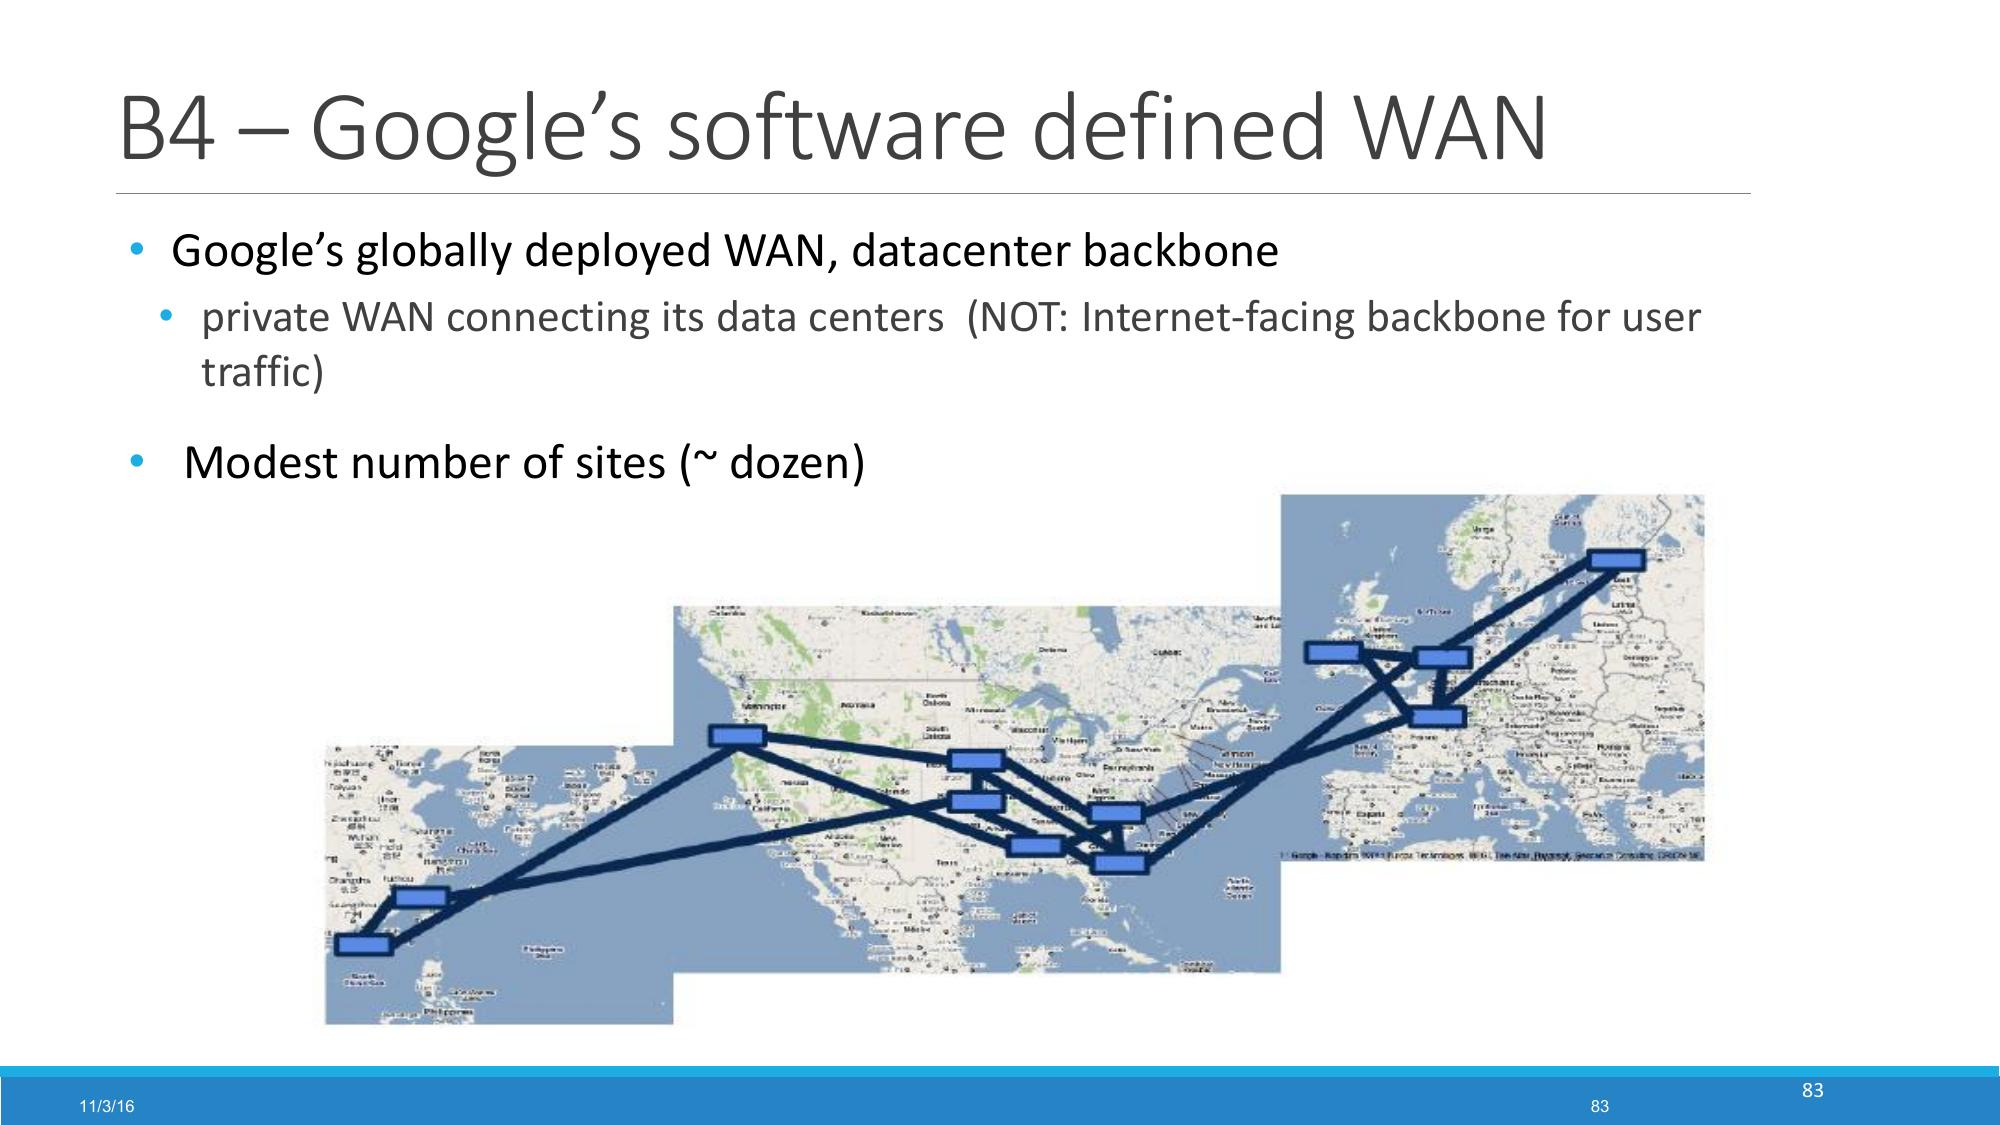
\includegraphics[keepaspectratio]{images/lezione-16-lab-sdn-applications-e-p4-language-img-01.jpg}}
\caption{La rete B4 connette una dozzina di siti (datacenter) in tutto
il mondo tramite link privati intercontinentali.}
\end{figure}

\begin{figure}
\centering
\pandocbounded{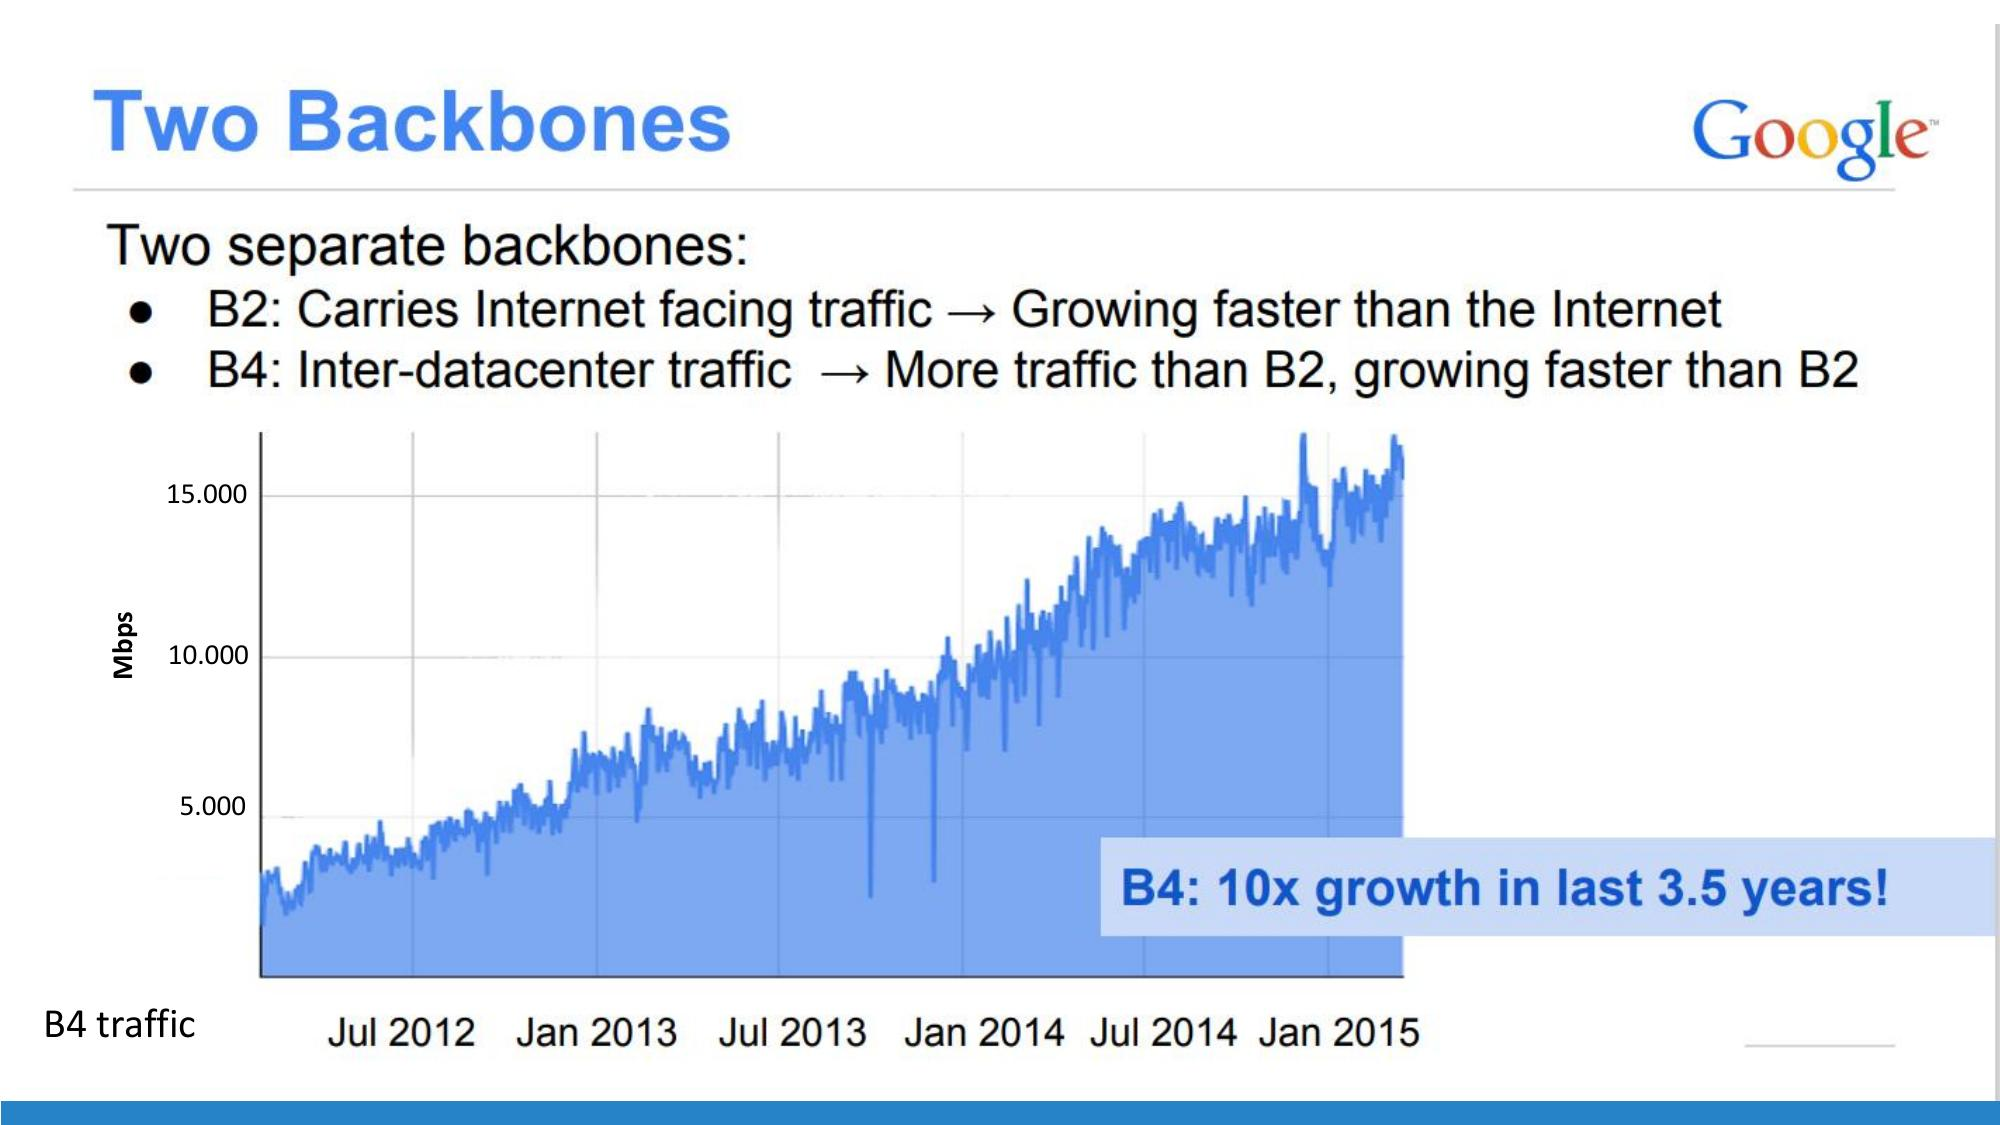
\includegraphics[keepaspectratio]{images/lezione-16-lab-sdn-applications-e-p4-language-img-02.jpg}}
\caption{Traffico B4 dal 2012 al 2015: crescita di 10x in 3.5 anni, con
B4 che supera B2 per volume.}
\end{figure}

\subsection{Caratteristiche del traffico
B4}\label{caratteristiche-del-traffico-b4}

Il traffico che percorre B4 non è omogeneo. Le slide distinguono tre
categorie principali, ordinate per sensibilità alla latenza e volume:

{\def\LTcaptype{none} % do not increment counter
\begin{longtable}[]{@{}
  >{\raggedright\arraybackslash}p{(\linewidth - 6\tabcolsep) * \real{0.2500}}
  >{\raggedright\arraybackslash}p{(\linewidth - 6\tabcolsep) * \real{0.2500}}
  >{\raggedright\arraybackslash}p{(\linewidth - 6\tabcolsep) * \real{0.2500}}
  >{\raggedright\arraybackslash}p{(\linewidth - 6\tabcolsep) * \real{0.2500}}@{}}
\toprule\noalign{}
\begin{minipage}[b]{\linewidth}\raggedright
Tipo di traffico
\end{minipage} & \begin{minipage}[b]{\linewidth}\raggedright
Volume
\end{minipage} & \begin{minipage}[b]{\linewidth}\raggedright
Sensibilità latenza
\end{minipage} & \begin{minipage}[b]{\linewidth}\raggedright
Priorità
\end{minipage} \\
\midrule\noalign{}
\endhead
\bottomrule\noalign{}
\endlastfoot
Replicazione dati utente verso datacenter remoti & Basso & Alta &
Alta \\
Accesso remoto a storage per computazione distribuita & Medio & Media &
Media \\
Sincronizzazione di stato tra datacenter (bulk transfer) & Alto & Bassa
& Bassa \\
\end{longtable}
}

Questa eterogeneità è cruciale: il traffico di tipo 3 è elastico ---
tollera riduzioni temporanee di banda e persino fallimenti --- e
costituisce la maggior parte del volume. Questo rende B4 \textbf{adatto
al traffic engineering aggressivo}: si può rimandare o rallentare il
traffico a bassa priorità per fare spazio a quello critico.

\begin{callouttip}{L’insight chiave di B4}

Il traffico inter-datacenter è prevalentemente \emph{bulk} ed
\emph{elastico}. A differenza del traffico utente, non ha bisogno di
garanzie di bassa latenza costante. Questo apre la strada a
ottimizzazioni aggressive della banda che sarebbero impossibili su una
WAN tradizionale.

\end{callouttip}

\subsection{Caratteristiche di progetto di
B4}\label{caratteristiche-di-progetto-di-b4}

B4 si distingue dalla WAN tradizionale per quattro proprietà
fondamentali.

La prima è la \textbf{domanda di banda elastica}: le applicazioni
tollerano failure temporanei e riduzioni di banda, il che permette di
ottimizzare l'utilizzo senza sacrificare l'esperienza utente.

La seconda è il \textbf{numero moderato di siti}: poche decine di siti
significa che le tabelle di routing restano piccole e gestibili --- non
serve la scalabilità da centinaia di migliaia di rotte tipica di un
router ISP.

La terza è il \textbf{controllo fine-grained delle applicazioni}: le
applicazioni stesse comunicano le loro priorità e possono controllare i
burst, eliminando la necessità di overprovisioning dei link.

La quarta è la \textbf{sensibilità al costo}: i link intercontinentali
privati sono estremamente costosi e devono essere utilizzati al 100\%
della capacità disponibile. Non ci si può permettere il lusso del
30--40\% di utilizzo tipico delle WAN tradizionali.

\begin{center}\rule{0.5\linewidth}{0.5pt}\end{center}

\subsection{Architettura SDN di B4}\label{architettura-sdn-di-b4}

La transizione di Google verso SDN è avvenuta in tre stadi progressivi,
che illustrano perfettamente la metodologia di migrazione graduale.

\subsubsection{Stadio 1 --- Rete di
partenza}\label{stadio-1-rete-di-partenza}

Nella configurazione iniziale, i \emph{site} (nodi WAN) comunicano tra
loro tramite protocolli distribuiti tradizionali: iBGP e ISIS per il
routing interno ai siti, eBGP tra i siti. I \emph{cluster} (reti
datacenter) sono collegati ai siti tramite router BGP. Il controllo è
interamente distribuito --- nessun controller centralizzato.

\begin{figure}
\centering
\pandocbounded{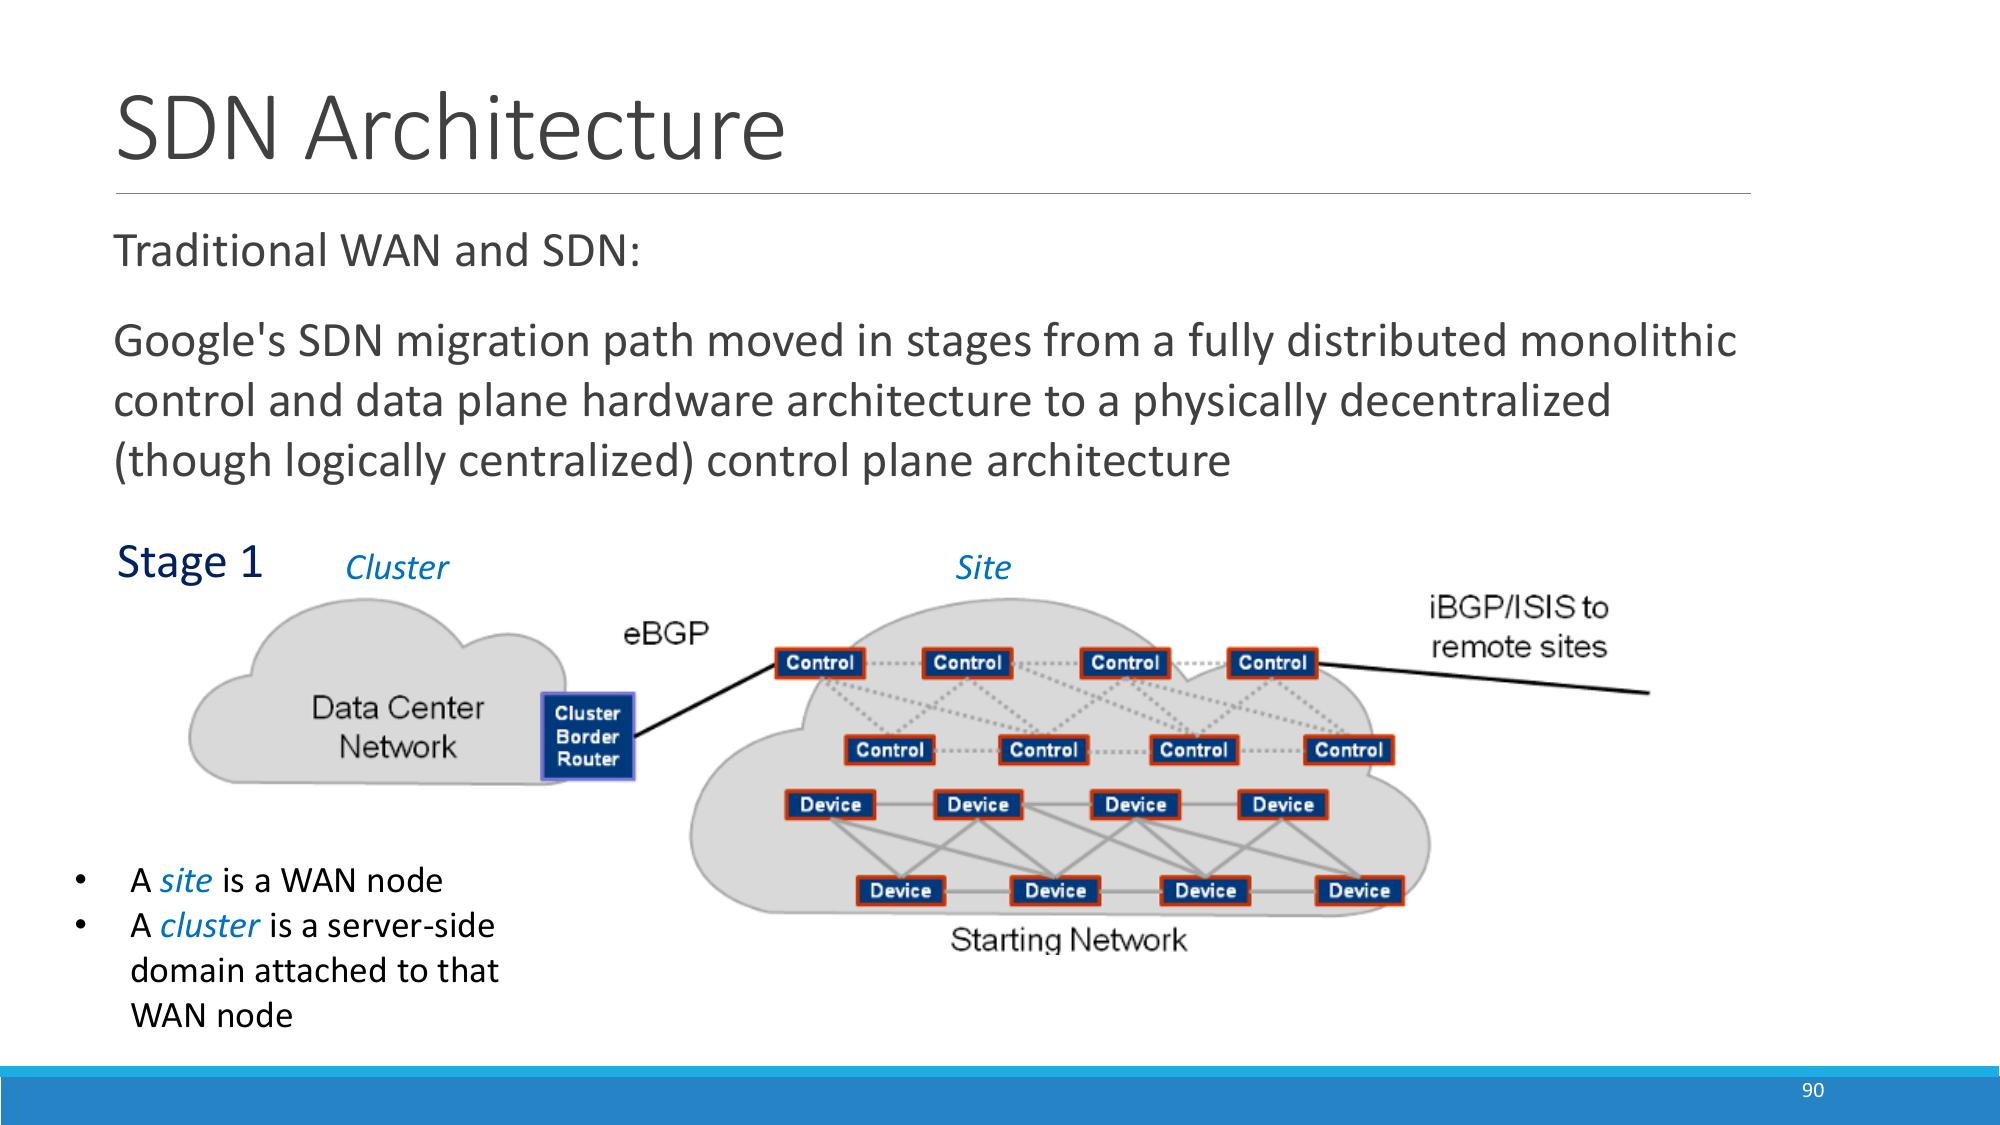
\includegraphics[keepaspectratio]{images/lezione-16-lab-sdn-applications-e-p4-language-img-03.jpg}}
\caption{Stage 1: la rete di partenza, con controllo distribuito basato
su BGP/ISIS. Un sito è un nodo WAN; un cluster è il dominio server
collegato a quel nodo.}
\end{figure}

\subsubsection{Stadio 2 --- Deployment parziale di
OpenFlow}\label{stadio-2-deployment-parziale-di-openflow}

Nella fase intermedia, viene introdotto per alcuni switch il controller
OpenFlow, affiancato da Quagga (il software di routing BGP/ISIS) e da un
modulo ``Glue'' che coordina i due sistemi. Il consenso tra istanze
ridondanti del controller è gestito tramite \textbf{Paxos}, garantendo
fault tolerance. La rete è in uno stato ibrido: alcuni switch sono già
controllati da OpenFlow, altri ancora dal piano di controllo distribuito
tradizionale.

\begin{figure}
\centering
\pandocbounded{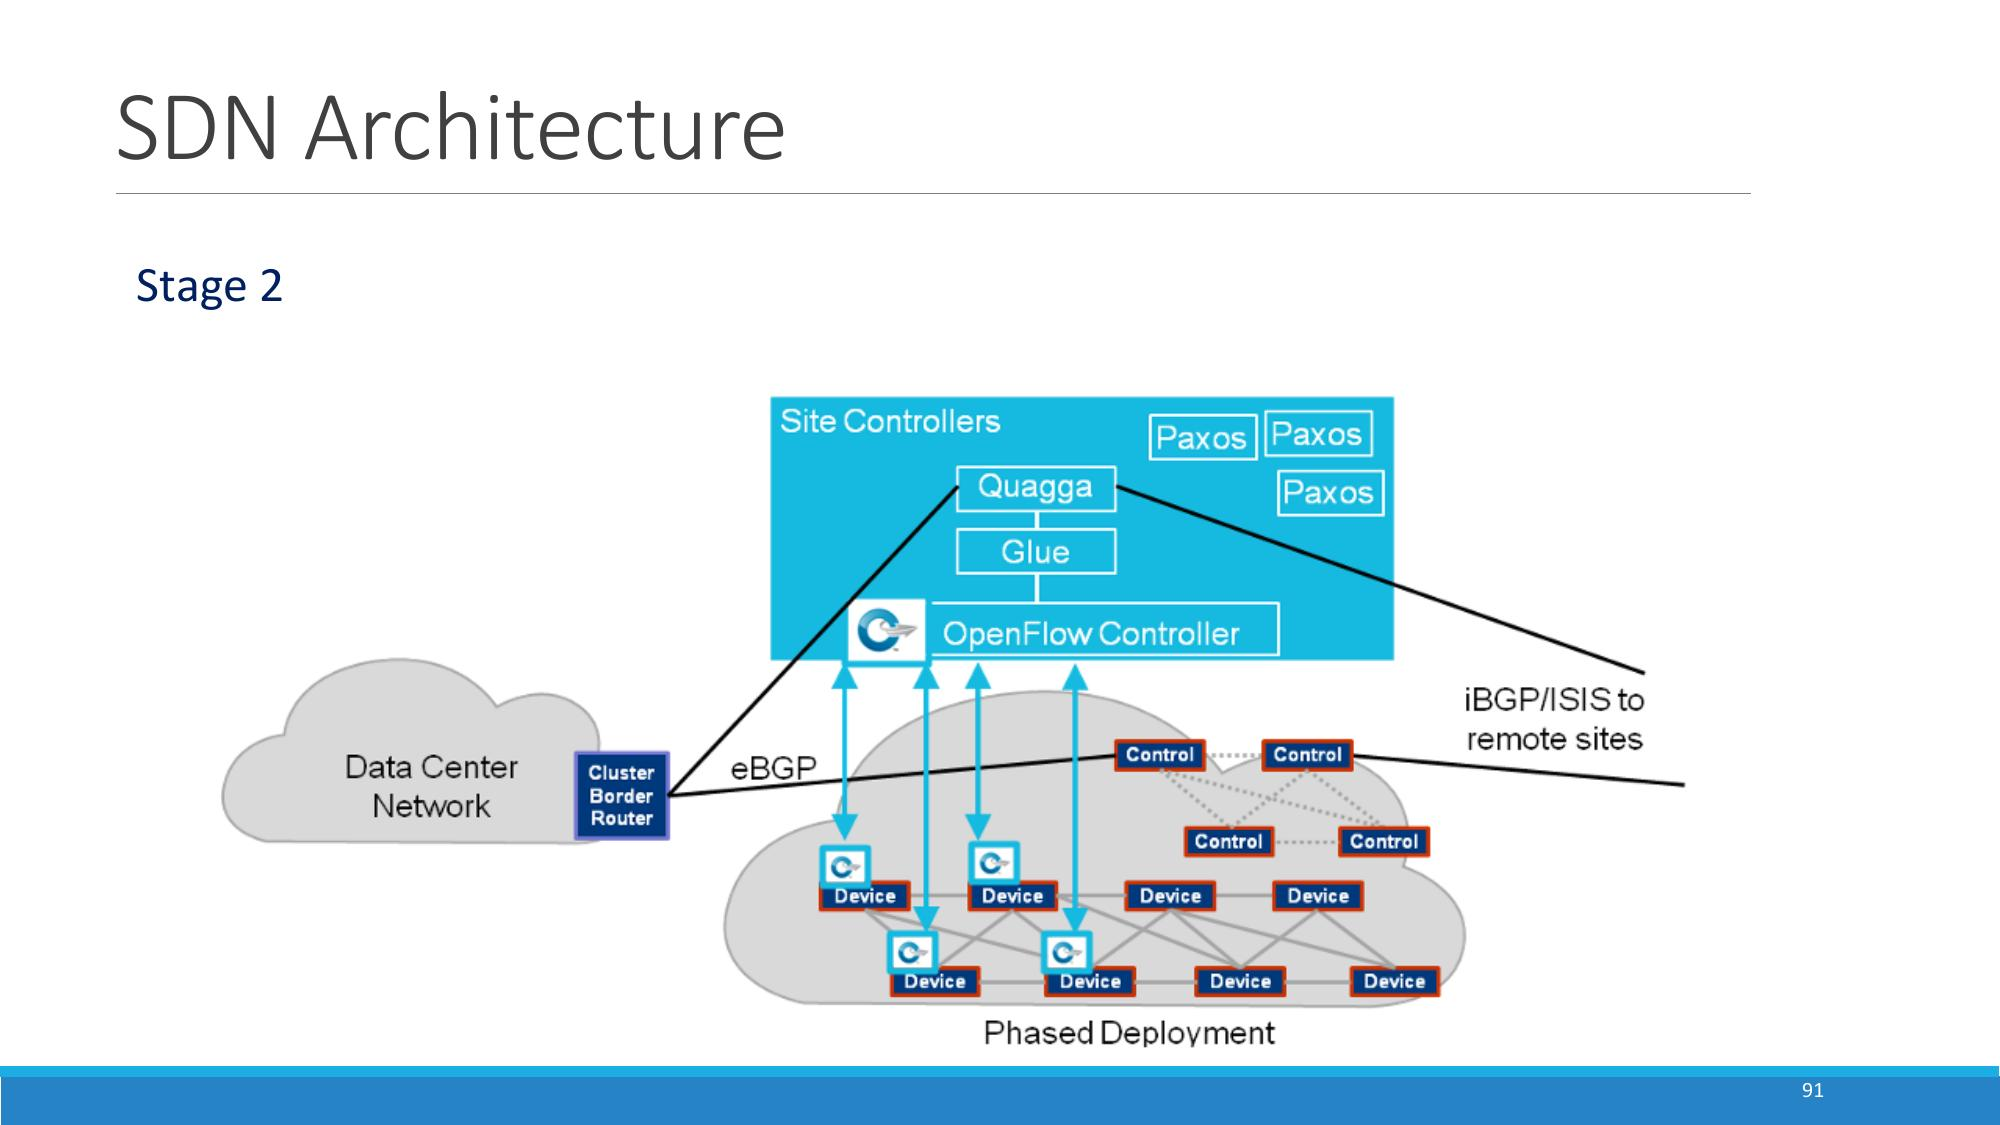
\includegraphics[keepaspectratio]{images/lezione-16-lab-sdn-applications-e-p4-language-img-04.jpg}}
\caption{Stage 2: deployment graduale. I Site Controllers con OpenFlow
coesistono con i nodi di controllo tradizionale. Paxos garantisce la
fault tolerance del controller.}
\end{figure}

\subsubsection{Stadio 3 --- Architettura
target}\label{stadio-3-architettura-target}

Nella configurazione finale, tutti gli switch sono controllati da
OpenFlow. Viene aggiunto il \textbf{Central TE Server} (Traffic
Engineering Server) come applicazione globale che ottimizza l'intera
rete. Il layer di controllo è fisicamente distribuito ma logicamente
centralizzato.

\begin{figure}
\centering
\pandocbounded{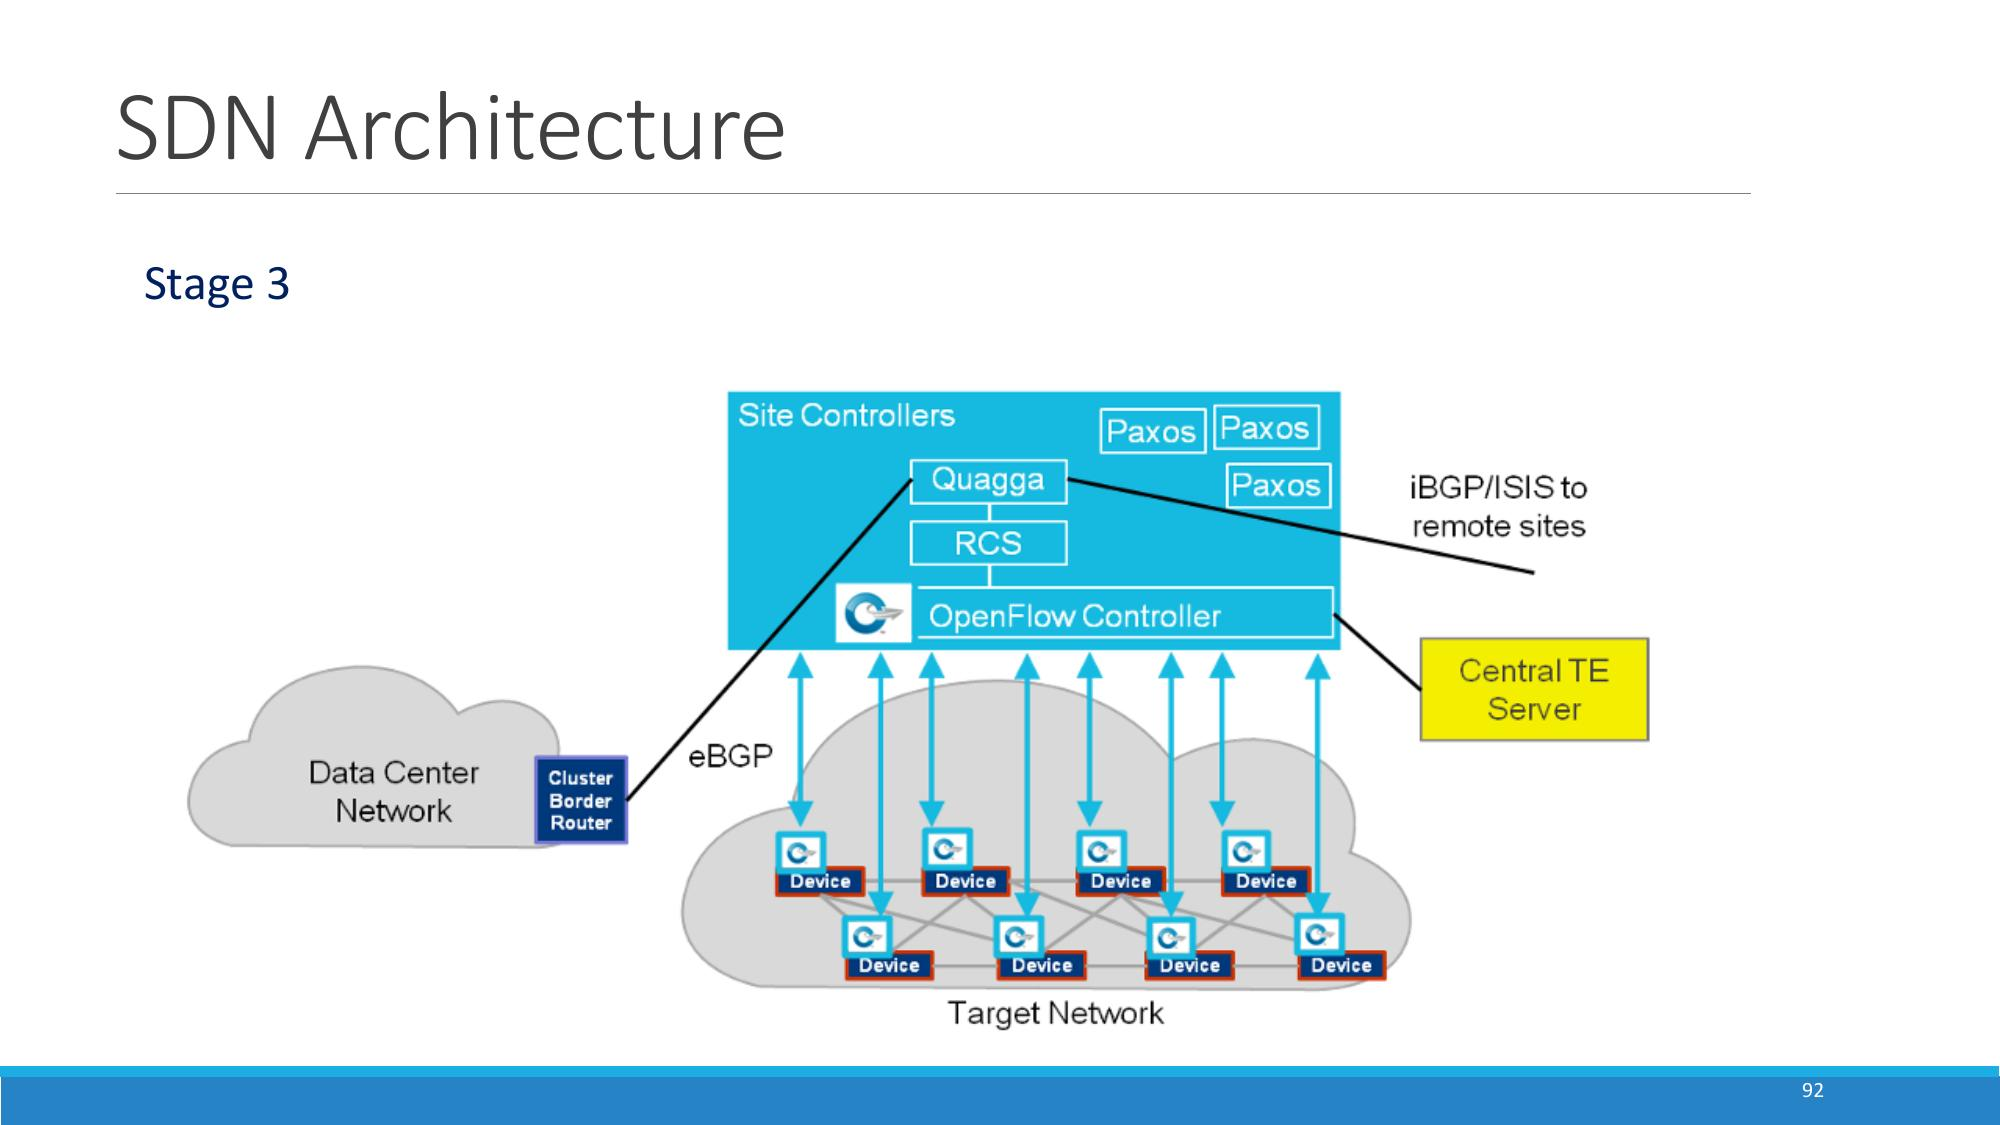
\includegraphics[keepaspectratio]{images/lezione-16-lab-sdn-applications-e-p4-language-img-05.jpg}}
\caption{Stage 3: rete target. Tutti i dispositivi sono controllati via
OpenFlow. Il Central TE Server fornisce ottimizzazione globale del
traffico.}
\end{figure}

\subsubsection{Integrazione con BGP e piano di controllo
tradizionale}\label{integrazione-con-bgp-e-piano-di-controllo-tradizionale}

Anche nell'architettura finale, BGP non scompare completamente. Ogni
cluster mantiene router BGP che si appoggiano agli switch B4 tramite
eBGP. BGP viene mantenuto per due ragioni pratiche: la familiarità degli
operatori con il protocollo (già in uso prima di SDN) e la necessità di
un deployment graduale e reversibile. BGP gestisce la
\emph{raggiungibilità} (reachability), mentre il \textbf{traffic
engineering} --- ovvero la selezione dei percorsi e l'allocazione della
banda --- è delegato interamente al sistema centralizzato SDN.

\begin{figure}
\centering
\pandocbounded{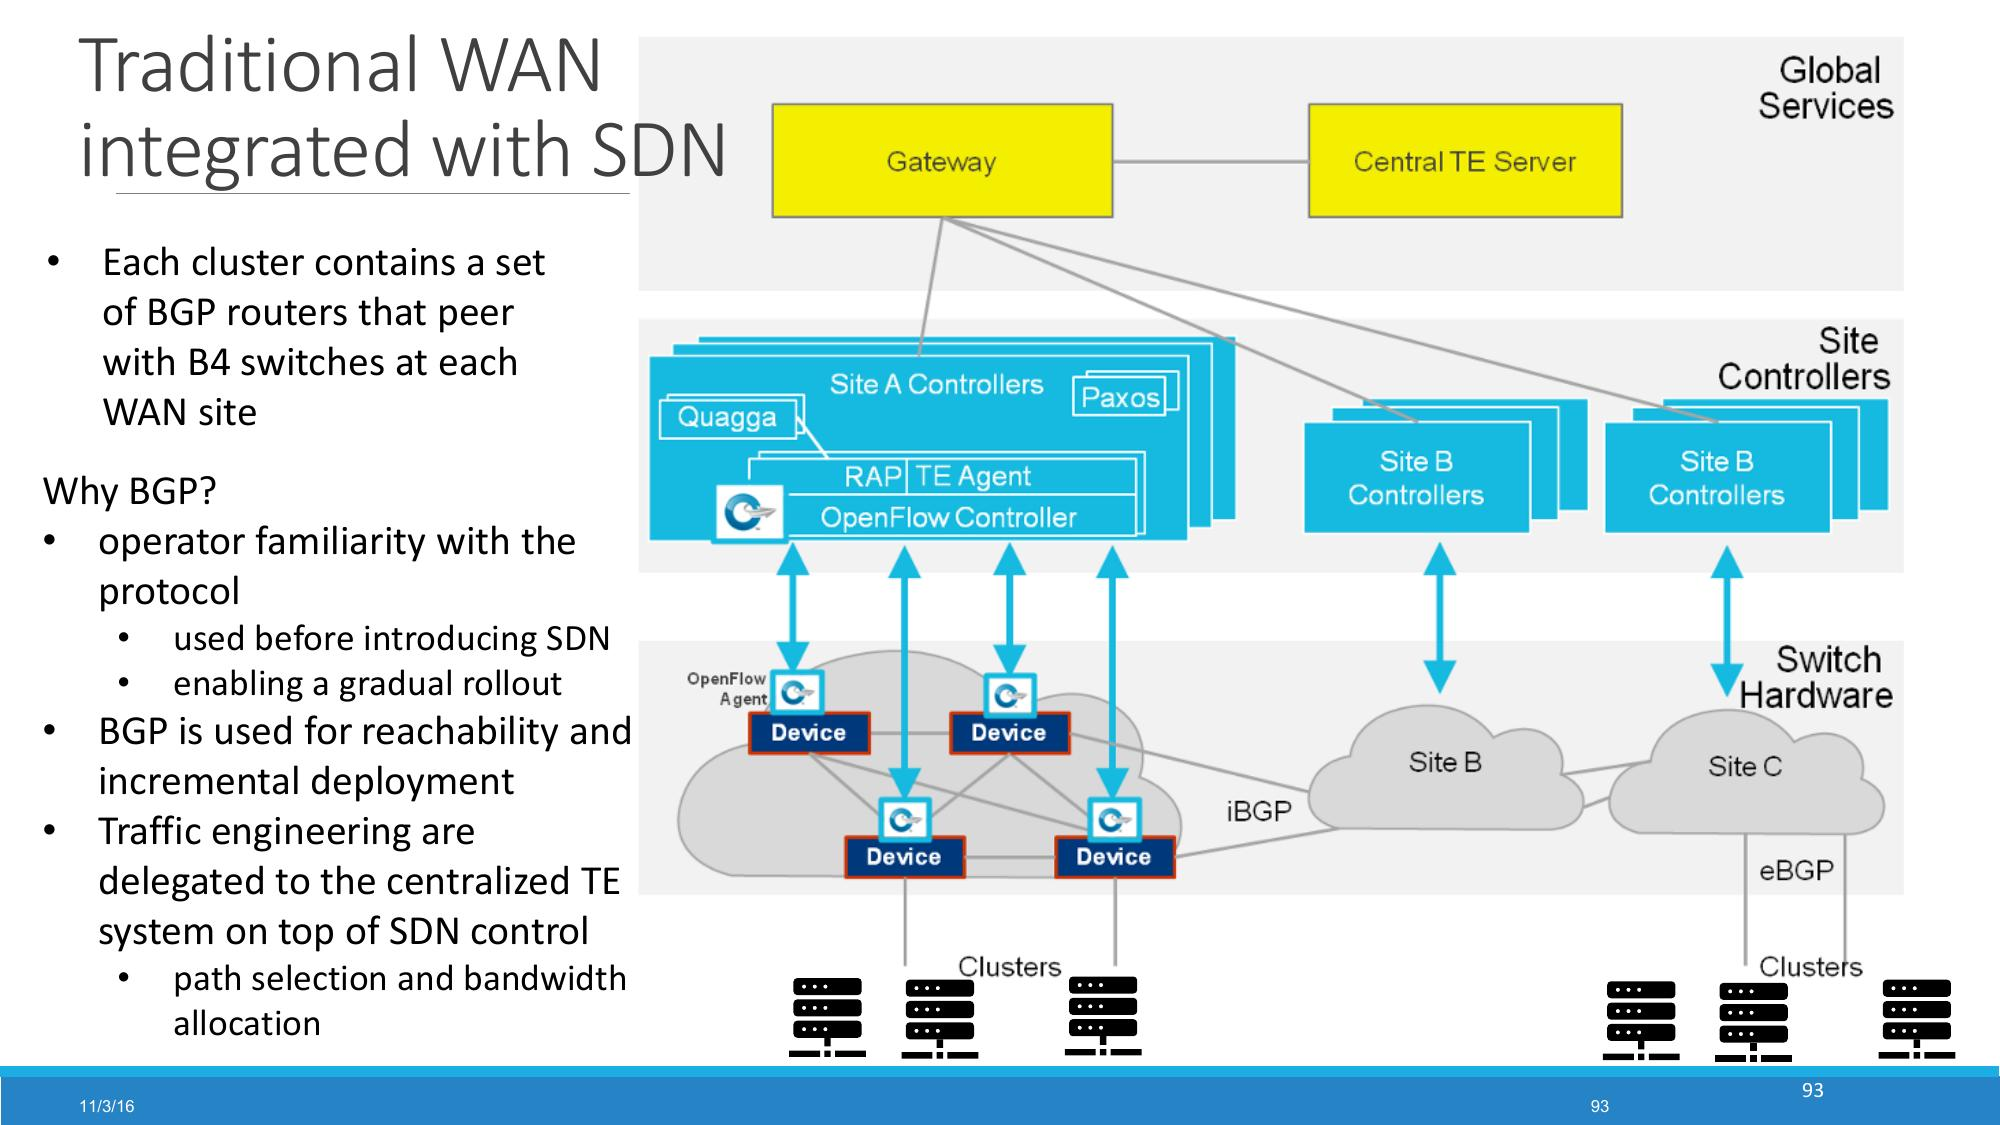
\includegraphics[keepaspectratio]{images/lezione-16-lab-sdn-applications-e-p4-language-img-06.jpg}}
\caption{L'architettura completa: BGP per la raggiungibilità, TE Server
centralizzato per l'ottimizzazione del traffico. Gateway, Site
Controllers e Switch Hardware interagiscono tramite OpenFlow.}
\end{figure}

\begin{calloutnote}{Perché mantenere BGP?}

BGP non è la scelta tecnicamente ``più pulita'' in un sistema SDN puro,
ma è mantenuto per due motivi pragmatici: (1) gli operatori lo conoscono
bene e lo usavano già prima di SDN, facilitando una transizione
graduale; (2) permette un rollout incrementale --- si può migrare un
sito alla volta senza interrompere il servizio.

\end{calloutnote}

\subsection{Panoramica dell'architettura
B4}\label{panoramica-dellarchitettura-b4}

L'architettura B4 si articola su tre layer sovrapposti.

Lo \textbf{Switch Hardware} è hardware custom di Google, progettato con
silicio commodity ma senza software di controllo complesso. La riduzione
del numero di siti elimina la necessità di grandi tabelle di forwarding;
il controllo applicativo fine-grained riduce la necessità di grandi
buffer.

Il \textbf{Control Layer} è composto da \emph{Network Control Servers}
(NCS) che ospitano sia gli \textbf{OpenFlow Controllers} (OFC) sia le
\textbf{Network Control Applications} (NCA). Gli OFC mantengono lo stato
della rete in base alle direttive delle NCA e agli eventi degli switch,
e istruiscono gli switch ad aggiornare le tabelle di forwarding. Per la
fault tolerance, un'istanza Paxos per sito elegge il controller primario
tra più repliche fisiche su server differenti.

Il \textbf{Global Layer} contiene le applicazioni logicamente
centralizzate: l'\textbf{SDN Gateway} e il \textbf{TE Server}. L'SDN
Gateway astrae i dettagli di OpenFlow e dell'hardware degli switch per
il TE Server --- ogni sito B4 può avere centinaia di porte fisiche, ma
il Gateway le aggrega in un'astrazione a livello di sito. Il TE Server
opera su questa visione globale per calcolare path e allocazioni di
banda.

\begin{center}\rule{0.5\linewidth}{0.5pt}\end{center}

\subsection{Traffic Engineering in B4}\label{traffic-engineering-in-b4}

Il Traffic Engineering (TE) è il meccanismo attraverso cui B4 realizza
l'utilizzo vicino al 100\% dei link. L'obiettivo del TE Server è
\textbf{condividere la banda tra applicazioni concorrenti},
possibilmente usando percorsi multipli.

\begin{figure}
\centering
\pandocbounded{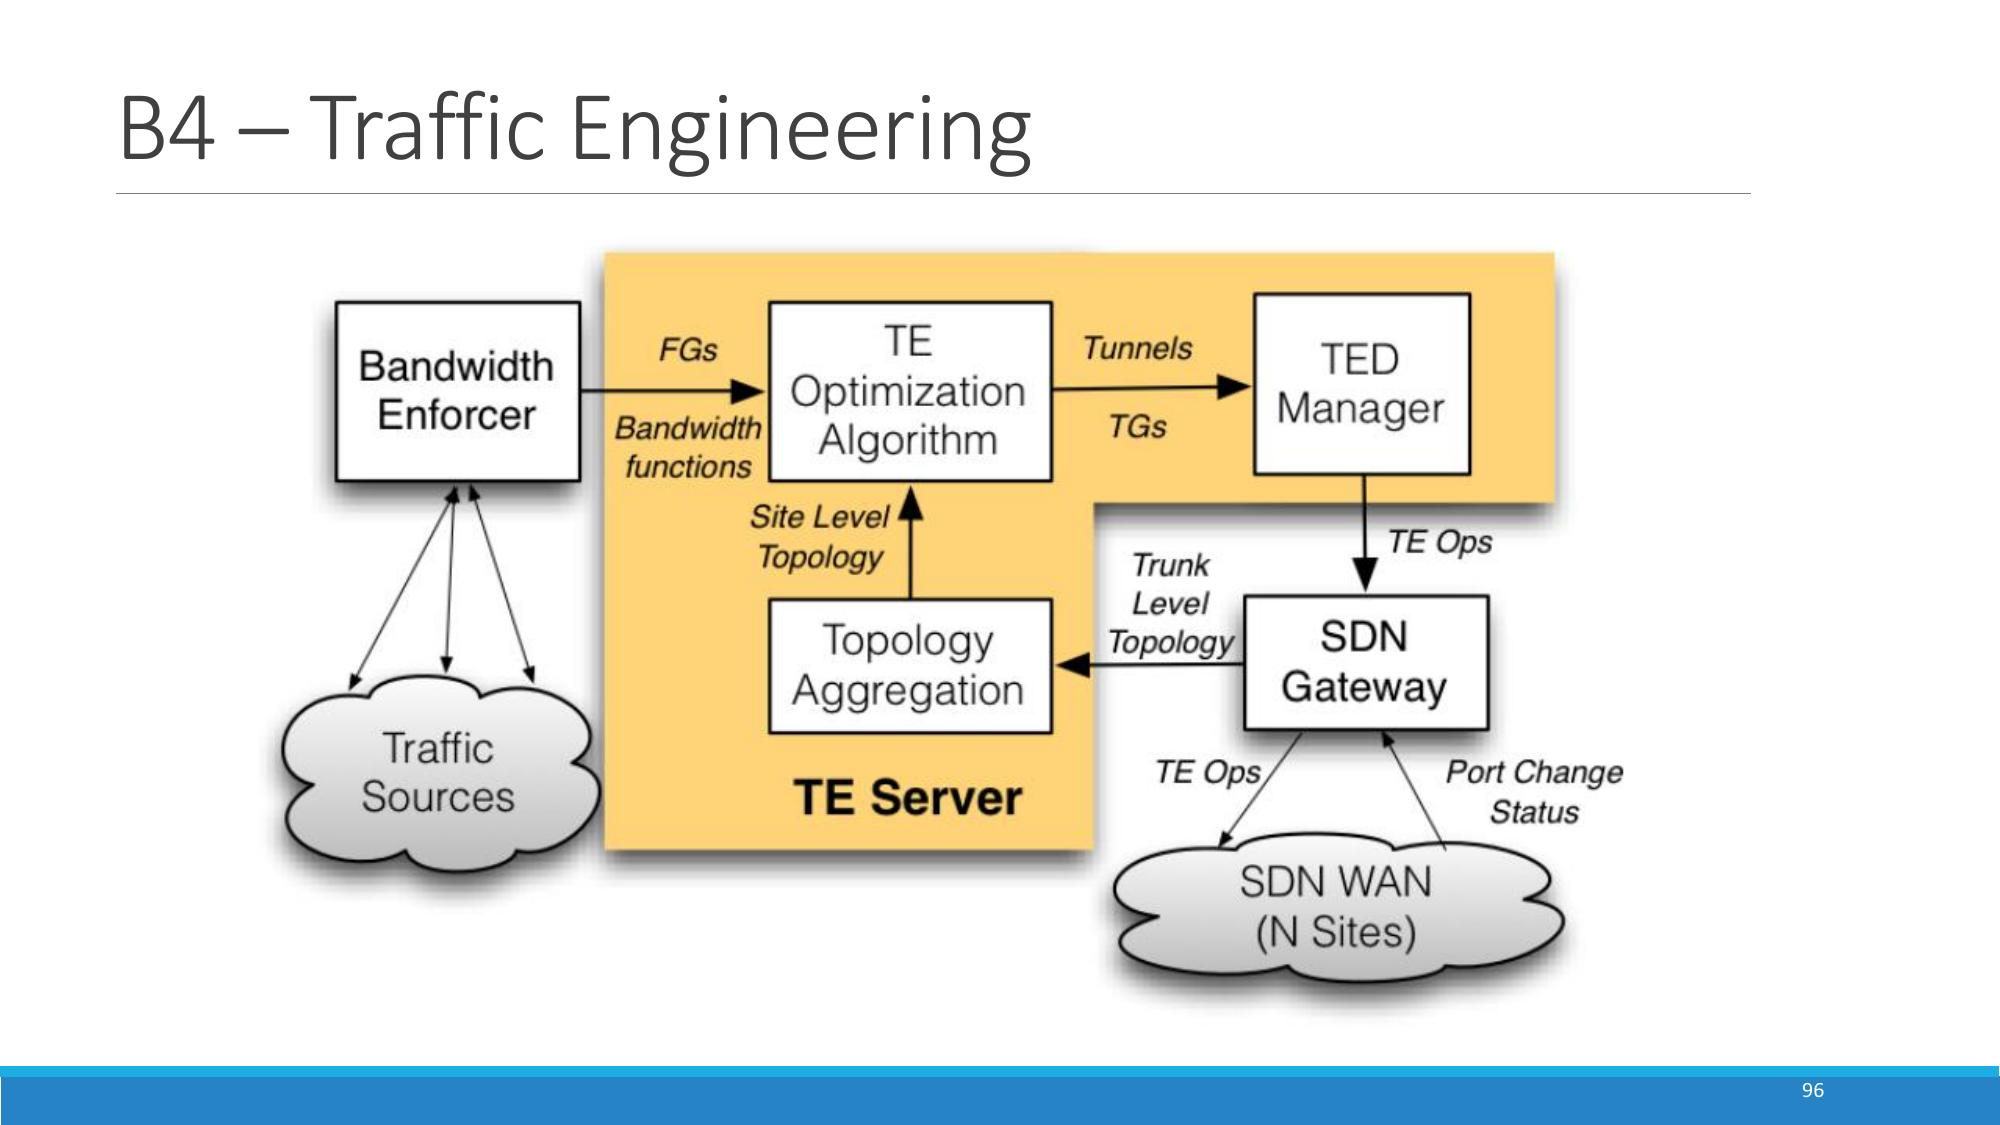
\includegraphics[keepaspectratio]{images/lezione-16-lab-sdn-applications-e-p4-language-img-07.jpg}}
\caption{Il TE Server riceve Flow Groups e funzioni di banda dal
Bandwidth Enforcer, ottimizza e produce Tunnels/Tunnel Groups che
vengono poi installati nella rete via SDN Gateway e OFC.}
\end{figure}

Il TE Server lavora su due astrazioni principali.

In \textbf{input} riceve: (1) la \emph{topologia di rete} come grafo di
siti e connessioni sito-a-sito, che riduce enormemente la dimensione del
problema rispetto a una topologia a livello di porta; (2) i \emph{flow
group} (FG), ciascuno definito come una tupla composta da sito sorgente,
sito destinazione e classe QoS. Il TE non lavora a livello di singola
applicazione --- aggrega il traffico per sito e classe di servizio. Il
\textbf{Bandwidth Enforcer} è un componente esterno che specifica le
funzioni di banda per ogni applicazione, derivate da pesi statici
configurati dall'amministratore.

In \textbf{output} produce: \emph{Tunnel} --- percorsi a livello di sito
come sequenze di siti (es. A→B→C), implementati tramite IP-in-IP
encapsulation --- e \emph{Tunnel Group} (TG), che mappano i flow group
sui tunnel disponibili.

\begin{calloutdefinition}{Tunnel in B4}

Un Tunnel rappresenta un percorso a livello di sito nella rete. È una
sequenza di siti (es. Amsterdam → Frankfurt → Warsaw) implementata con
incapsulamento IP-in-IP. Non coincide con un link fisico: può
attraversare più switch e link interni a ogni sito.

\end{calloutdefinition}

I Tunnel Group e i relativi Tunnel e Flow Group vengono inviati dall'SDN
Gateway agli OFC, che li installano negli switch via OpenFlow.

\subsubsection{Forwarding Multipath}\label{forwarding-multipath}

Per sfruttare pienamente la banda disponibile, B4 utilizza il
\textbf{forwarding multipath}: un flusso destinato a una subnet può
essere distribuito su più tunnel in parallelo. Lo switch usa una
funzione di hash sugli header del pacchetto (modulo il numero di entry
ACL) per distribuire equamente i flussi tra i tunnel disponibili,
garantendo che pacchetti dello stesso flusso seguano lo stesso percorso
(evitando riordinamento).

\begin{figure}
\centering
\pandocbounded{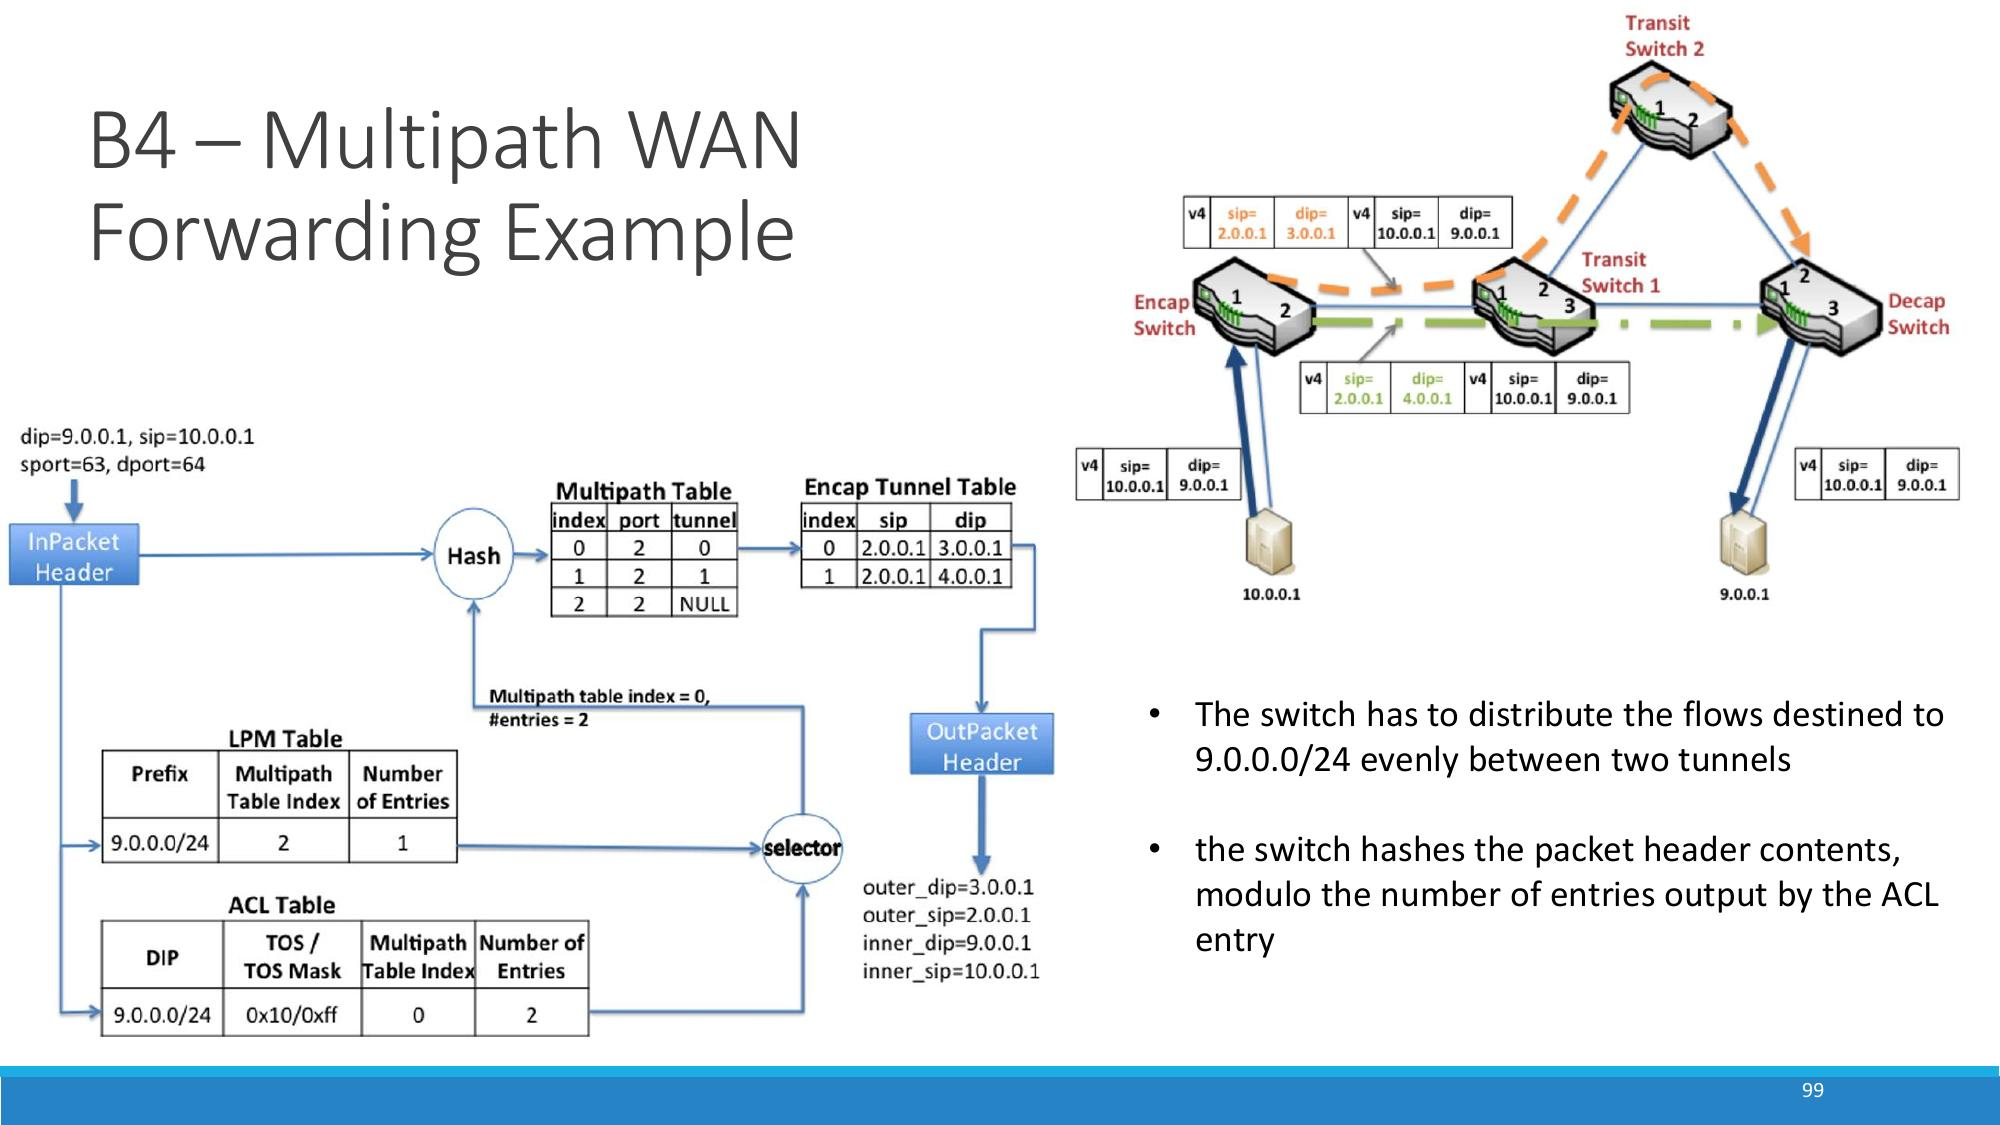
\includegraphics[keepaspectratio]{images/lezione-16-lab-sdn-applications-e-p4-language-img-08.jpg}}
\caption{Esempio di forwarding multipath: i flussi verso 9.0.0.0/24
vengono distribuiti equamente tra due tunnel tramite hash degli header
del pacchetto.}
\end{figure}

\begin{calloutnote}{Risultati di B4}

Grazie all'architettura SDN, Google ha raggiunto un utilizzo dei link
vicino al \textbf{100\%} per i carichi elastici --- contro il 30--40\%
delle WAN tradizionali. Questo ha permesso di ridurre costi e
complessità dell'infrastruttura, eliminando il sovrapprovisionamento da
2--3x. Ulteriori miglioramenti successivi hanno introdotto topologie
gerarchiche e algoritmi TE decentralizzati per migliorare scalabilità e
disponibilità.

\end{calloutnote}

\begin{center}\rule{0.5\linewidth}{0.5pt}\end{center}

\section{Verso un Data Plane
Programmabile}\label{verso-un-data-plane-programmabile}

\subsection{Limiti di OpenFlow}\label{limiti-di-openflow}

OpenFlow ha dimostrato il valore della separazione tra control plane e
data plane, ma presenta limiti intrinseci al crescere delle esigenze. Il
protocollo è nato semplice --- circa 12 header field --- ma la specifica
è cresciuta fino a \textasciitilde40 campi, aumentando la complessità.
Soprattutto, i datacenter moderni richiedono nuove forme di
encapsulamento dei pacchetti (VXLAN, NVGRE, ecc.) che OpenFlow non
supporta in modo flessibile.

Il problema più profondo è concettuale: la vera programmabilità di rete
richiederebbe la capacità di definire e modificare sia gli algoritmi del
control plane sia quelli del \textbf{data plane}. Gli operatori di rete
dovrebbero poter definire entrambi autonomamente, senza coinvolgere i
progettisti originali dell'hardware. OpenFlow permette di
\emph{installare regole} nel data plane, ma non di \emph{riprogrammare}
il data plane stesso.

\begin{callouttip}{La distinzione cruciale}

OpenFlow controlla \emph{cosa fanno} le tabelle di un data plane fisso.
P4 permette di definire \emph{come è fatto} il data plane stesso ---
quali header riconoscere, come processarli, quali azioni eseguire.

\end{callouttip}

\begin{center}\rule{0.5\linewidth}{0.5pt}\end{center}

\section{P4 Language}\label{p4-language}

\subsection{Cos'è P4}\label{cosuxe8-p4}

\textbf{P4} (\emph{Programming Protocol-Independent Packet Processors})
è un linguaggio di programmazione \emph{domain-specific} progettato per
dispositivi di rete. Il suo nome cattura l'essenza del progetto:
permette di programmare il processamento dei pacchetti in modo
indipendente dal protocollo sottostante.

P4 estende il paradigma match-action introdotto da OpenFlow, ma lo porta
a un livello superiore: invece di installare regole in tabelle
predefinite dall'hardware, con P4 il programmatore \textbf{definisce le
tabelle stesse}, i campi degli header da estrarre, le azioni possibili e
il flusso di controllo tra le tabelle.

\begin{calloutdefinition}{P4 — Proprietà fondamentali}

Un programma P4 descrive integralmente il comportamento atteso nel data
plane: - \textbf{Headers}: tutti gli header dei pacchetti e i campi
rilevanti per il matching - \textbf{Actions}: l'insieme di tutte le
azioni possibili supportate dalle tabelle - \textbf{Tables}: l'insieme
delle tabelle di matching e il flusso di controllo tra esse

In aggiunta agli header standard, i progettisti di rete possono definire
header per protocolli personalizzati.

\end{calloutdefinition}

P4 è stato concepito nel 2013 da un team accademico-industriale e
presentato all'ACM SIGCOMM 2014. La standardizzazione è coordinata dal
\textbf{P4 Language Consortium} (specifiche su \texttt{p4.org/specs}).

\subsection{Vantaggi e applicazioni di
P4}\label{vantaggi-e-applicazioni-di-p4}

P4 permette di \textbf{personalizzare il processamento dei pacchetti
senza modifiche hardware}, accelerando drasticamente il ciclo di
innovazione dei protocolli di rete. Le applicazioni principali
includono: SDN avanzato, monitoring e telemetria di rete,
implementazioni custom di sicurezza e firewall.

Il vantaggio competitivo rispetto all'approccio tradizionale è la
separazione tra il \emph{cosa} (il programma P4, scritto dall'utente) e
il \emph{come} (l'hardware o il compilatore, forniti dal vendor): lo
stesso programma può essere compilato per switch P4, SmartNIC, o
software su host.

\subsection{Compilazione e target P4}\label{compilazione-e-target-p4}

\begin{figure}
\centering
\pandocbounded{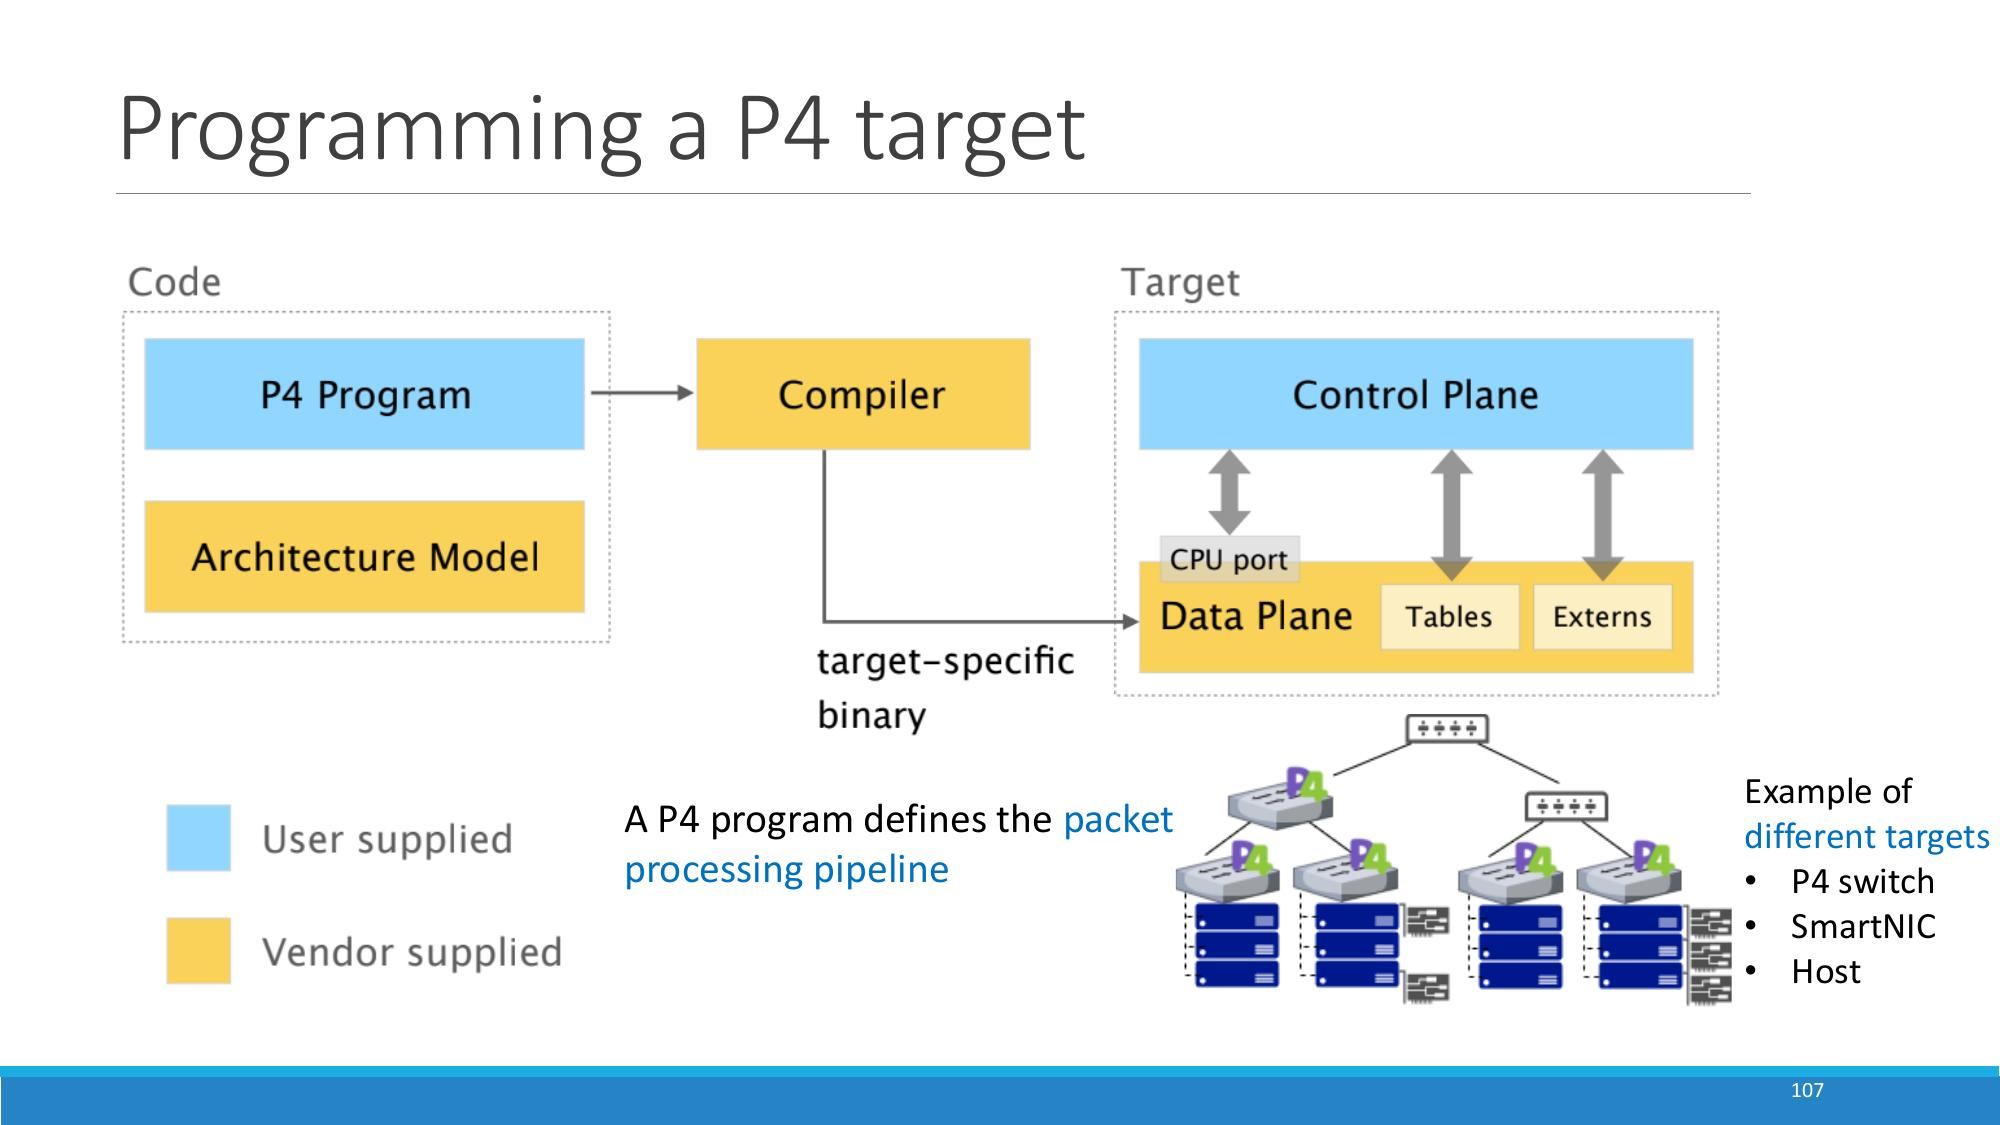
\includegraphics[keepaspectratio]{images/lezione-16-lab-sdn-applications-e-p4-language-img-09.jpg}}
\caption{Il programmatore scrive un P4 Program; il compilatore
vendor-specifico genera una configurazione del data plane e un'API per
il control plane (P4Runtime).}
\end{figure}

Un programma P4 viene scritto dal programmatore in termini
dell'\textbf{Architecture Model} --- una specifica astratta del target,
fornita dal vendor. Il \textbf{compilatore P4}, anch'esso
vendor-specifico, prende in input il programma e il modello
architetturale e produce:

\begin{itemize}
\tightlist
\item
  Una \textbf{configurazione del data plane} che implementa la logica di
  forwarding descritta nel programma.
\item
  Un'\textbf{API} per gestire lo stato degli oggetti del data plane dal
  control plane.
\end{itemize}

L'interazione a runtime tra control plane e data plane avviene tramite
\textbf{P4Runtime}, una specifica standard per controllare gli elementi
del data plane definiti da un programma P4. Il control plane popola le
tabelle con le regole; quando arriva un match, l'azione selezionata
viene eseguita con i parametri specificati dalla regola corrispondente.

I target supportati includono switch P4, SmartNIC e host software --- la
stessa logica di forwarding può essere eseguita su hardware diversissimi
semplicemente ricompilando.

\subsection{Struttura di un programma
P4}\label{struttura-di-un-programma-p4}

Un programma P4 è composto da tre componenti principali, che
corrispondono alle tre fasi del ciclo di vita di un pacchetto nel data
plane.

\begin{figure}
\centering
\pandocbounded{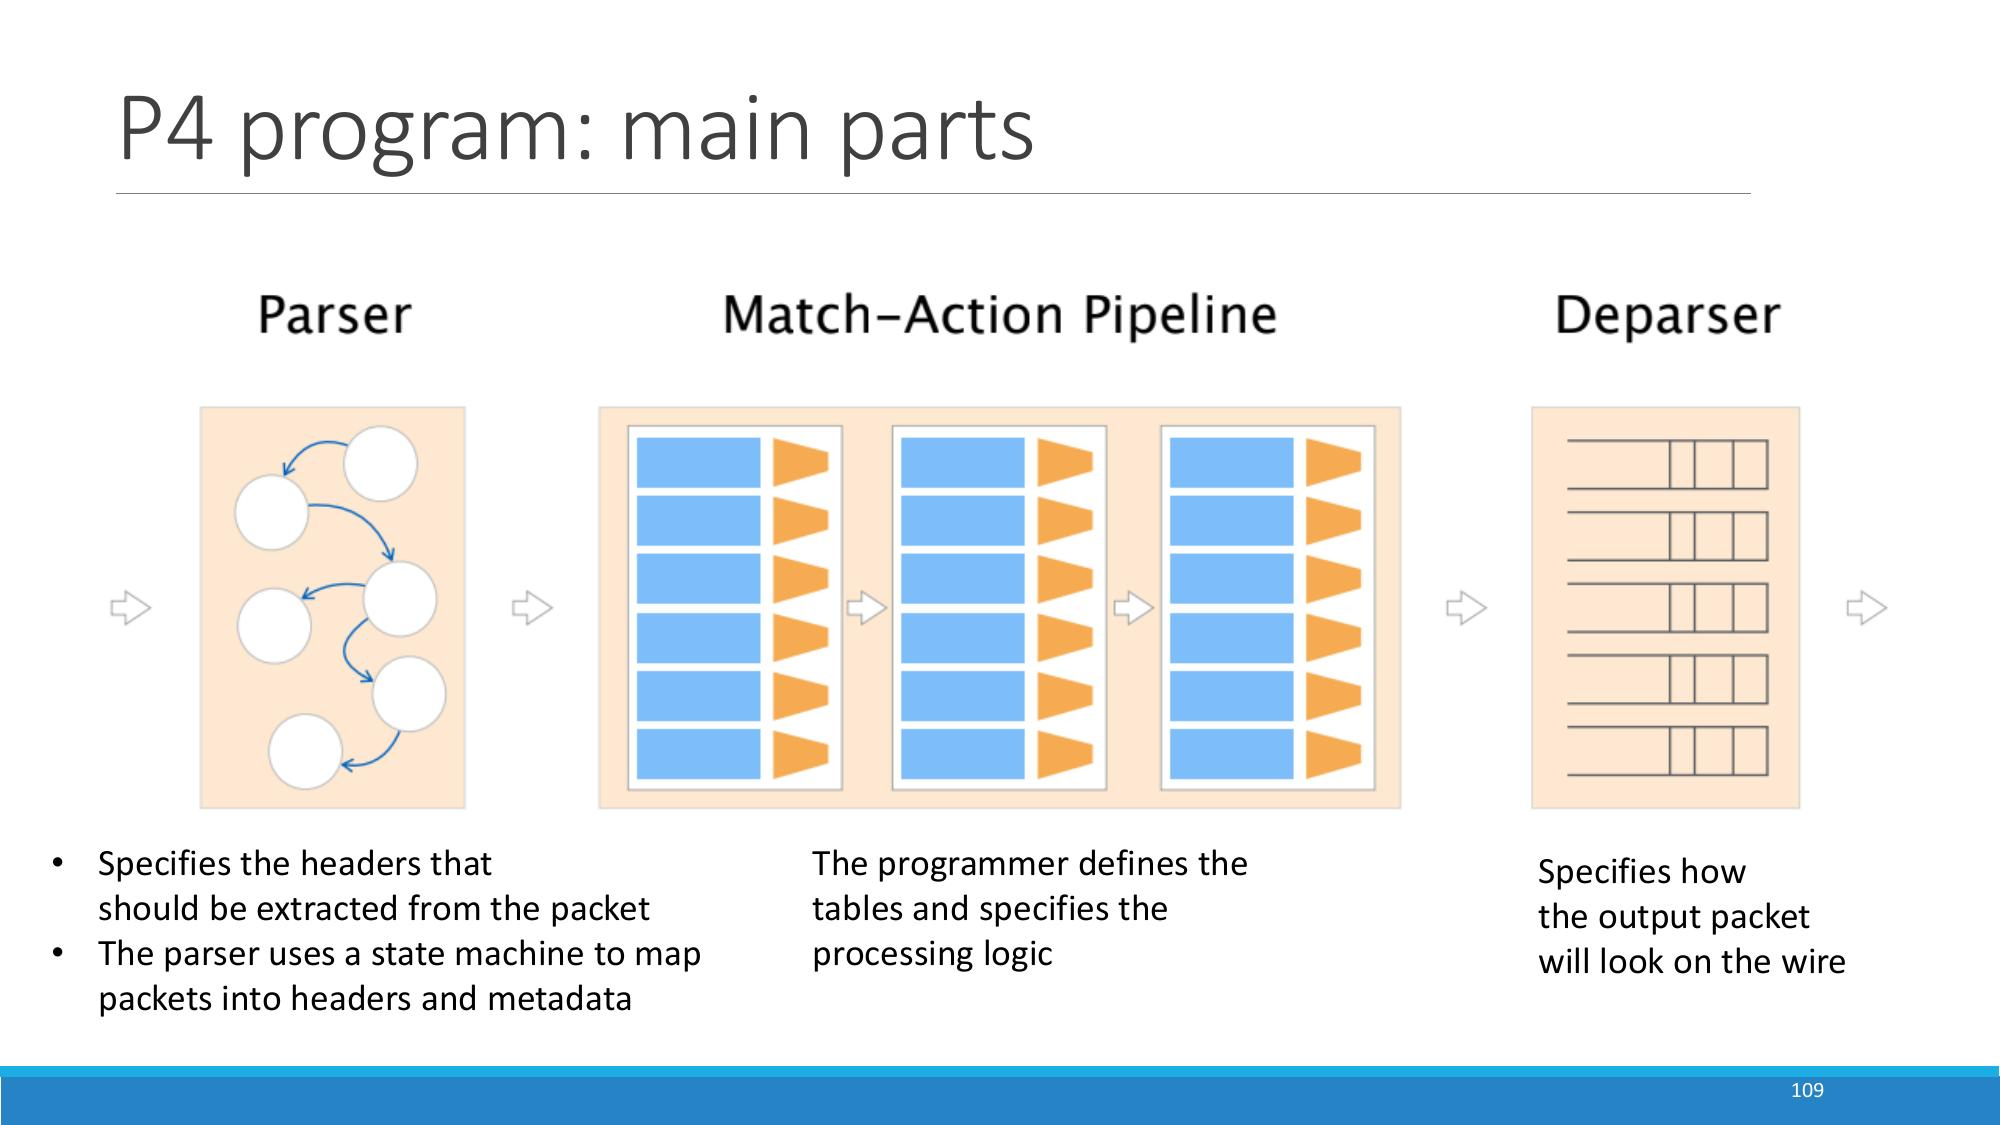
\includegraphics[keepaspectratio]{images/lezione-16-lab-sdn-applications-e-p4-language-img-10.jpg}}
\caption{Pipeline P4: il Parser estrae gli header (state machine), la
Match-Action Pipeline applica le regole, il Deparser ricostruisce il
pacchetto per il wire.}
\end{figure}

\subsubsection{Parser}\label{parser}

Il \textbf{Parser} specifica come estrarre gli header dai pacchetti in
ingresso. Usa una \textbf{macchina a stati} per mappare il flusso di
byte in strutture header e metadata. Per esempio, si parte dallo stato
\texttt{start}, si estrae l'header Ethernet, e in base al campo
\texttt{eth\_type} si transita allo stato \texttt{parse\_ipv4} (per
pacchetti IP) oppure si accetta direttamente il pacchetto.

\begin{Shaded}
\begin{Highlighting}[]
\NormalTok{header ethernet\_t \{}
\NormalTok{    bit\textless{}48\textgreater{} dst\_addr;}
\NormalTok{    bit\textless{}48\textgreater{} src\_addr;}
\NormalTok{    bit\textless{}16\textgreater{} eth\_type;}
\NormalTok{\}}

\NormalTok{header ipv4\_t \{}
\NormalTok{    bit\textless{}4\textgreater{}  version;}
\NormalTok{    bit\textless{}4\textgreater{}  ihl;}
\NormalTok{    bit\textless{}8\textgreater{}  diffserv;}
\NormalTok{    bit\textless{}16\textgreater{} totalLen;}
\NormalTok{    bit\textless{}16\textgreater{} identification;}
\NormalTok{    bit\textless{}3\textgreater{}  flags;}
\NormalTok{    bit\textless{}13\textgreater{} fragOffset;}
\NormalTok{    bit\textless{}8\textgreater{}  ttl;}
\NormalTok{    bit\textless{}8\textgreater{}  protocol;}
\NormalTok{    bit\textless{}16\textgreater{} hdrChecksum;}
\NormalTok{    bit\textless{}32\textgreater{} srcAddr;}
\NormalTok{    bit\textless{}32\textgreater{} dstAddr;}
\NormalTok{\}}

\NormalTok{parser MyParser(packet\_in packet,}
\NormalTok{                out headers\_t hdr,}
\NormalTok{                inout metadata\_t meta) \{}

\NormalTok{    state start \{}
\NormalTok{        packet.extract(hdr.ethernet);}
\NormalTok{        transition select(hdr.ethernet.eth\_type) \{}
\NormalTok{            0x0800: parse\_ipv4;}
\NormalTok{            default: accept;}
\NormalTok{        \}}
\NormalTok{    \}}

\NormalTok{    state parse\_ipv4 \{}
\NormalTok{        packet.extract(hdr.ipv4);}
\NormalTok{        transition accept;}
\NormalTok{    \}}
\NormalTok{\}}
\end{Highlighting}
\end{Shaded}

Gli header vengono dichiarati con campi a larghezza fissa (es.
\texttt{bit\textless{}48\textgreater{}} per un MAC address). La
struttura \texttt{headers\_t} li raggruppa in un unico oggetto che
attraversa tutta la pipeline.

\subsubsection{Match-Action Pipeline}\label{match-action-pipeline}

Il programmatore definisce le \textbf{tabelle di matching} e la logica
di processamento. Ogni tabella specifica i campi su cui fare match, le
azioni possibili, e la dimensione massima. Quando un pacchetto arriva,
viene confrontato con le regole della tabella (installate dal control
plane); se trova un match, l'azione associata viene eseguita con i
parametri specificati dalla regola.

\begin{calloutnote}{Differenza rispetto a OpenFlow}

In OpenFlow, le tabelle sono fisse nell'hardware: l'operatore può solo
popolarle con regole. In P4, le tabelle stesse sono definite nel
programma: il programmatore decide quante tabelle ci sono, su quali
campi fare match, e quali azioni sono disponibili. Questo abilita
protocolli completamente nuovi senza modificare l'hardware.

\end{calloutnote}

\subsubsection{Deparser}\label{deparser}

Il \textbf{Deparser} specifica come ricostruire il pacchetto per
l'output sul wire. Definisce l'ordine in cui gli header modificati
vengono serializzati nel flusso di byte in uscita, permettendo anche di
aggiungere o rimuovere header (es. per encapsulamento/decapsulamento).

\begin{calloutnote}{Sintesi del modello P4}

P4 porta la programmabilità al data plane con un modello coerente:
Parser (deserializzazione) → Match-Action Pipeline (processamento) →
Deparser (serializzazione). Il control plane (via P4Runtime) si occupa
solo di popolare le tabelle; tutta la logica di parsing e azione è
definita staticamente nel programma P4 e compilata nell'hardware.

\end{calloutnote}

\begin{center}\rule{0.5\linewidth}{0.5pt}\end{center}

\section{Service Function Chaining}\label{service-function-chaining}

\subsection{Il problema: comporre funzioni di
rete}\label{il-problema-comporre-funzioni-di-rete}

Le reti moderne non applicano ai pacchetti una singola trasformazione,
ma una sequenza di elaborazioni: un pacchetto che entra da Internet può
dover attraversare un firewall, un sistema di intrusion detection (IDS),
e un load balancer prima di raggiungere il server applicativo. Ciascuna
di queste elaborazioni è una \textbf{Network Function} --- una capacità
di processamento dei pacchetti fornita da un dispositivo di rete.

\begin{calloutdefinition}{Service Function Chaining (SFC)}

Il \textbf{Service Function Chaining} è il paradigma per definire e
gestire servizi di rete come catene ordinate di funzioni di rete. Una
catena definisce come un flusso di traffico deve essere processato per
raggiungere obiettivi di sicurezza, performance o QoS.

Esempi di funzioni di rete: NAT, firewall, IDS, DNS, caching, DDoS
protection, load balancer.

\end{calloutdefinition}

Nelle reti tradizionali, le service chain sono implementate
topologicamente: i dispositivi fisici sono cablati in sequenza, e il
traffico li attraversa nell'ordine fisico. Questo rende l'aggiornamento
o il cambiamento delle chain estremamente rigido e costoso.

\subsection{SFC con SDN}\label{sfc-con-sdn}

\begin{figure}
\centering
\pandocbounded{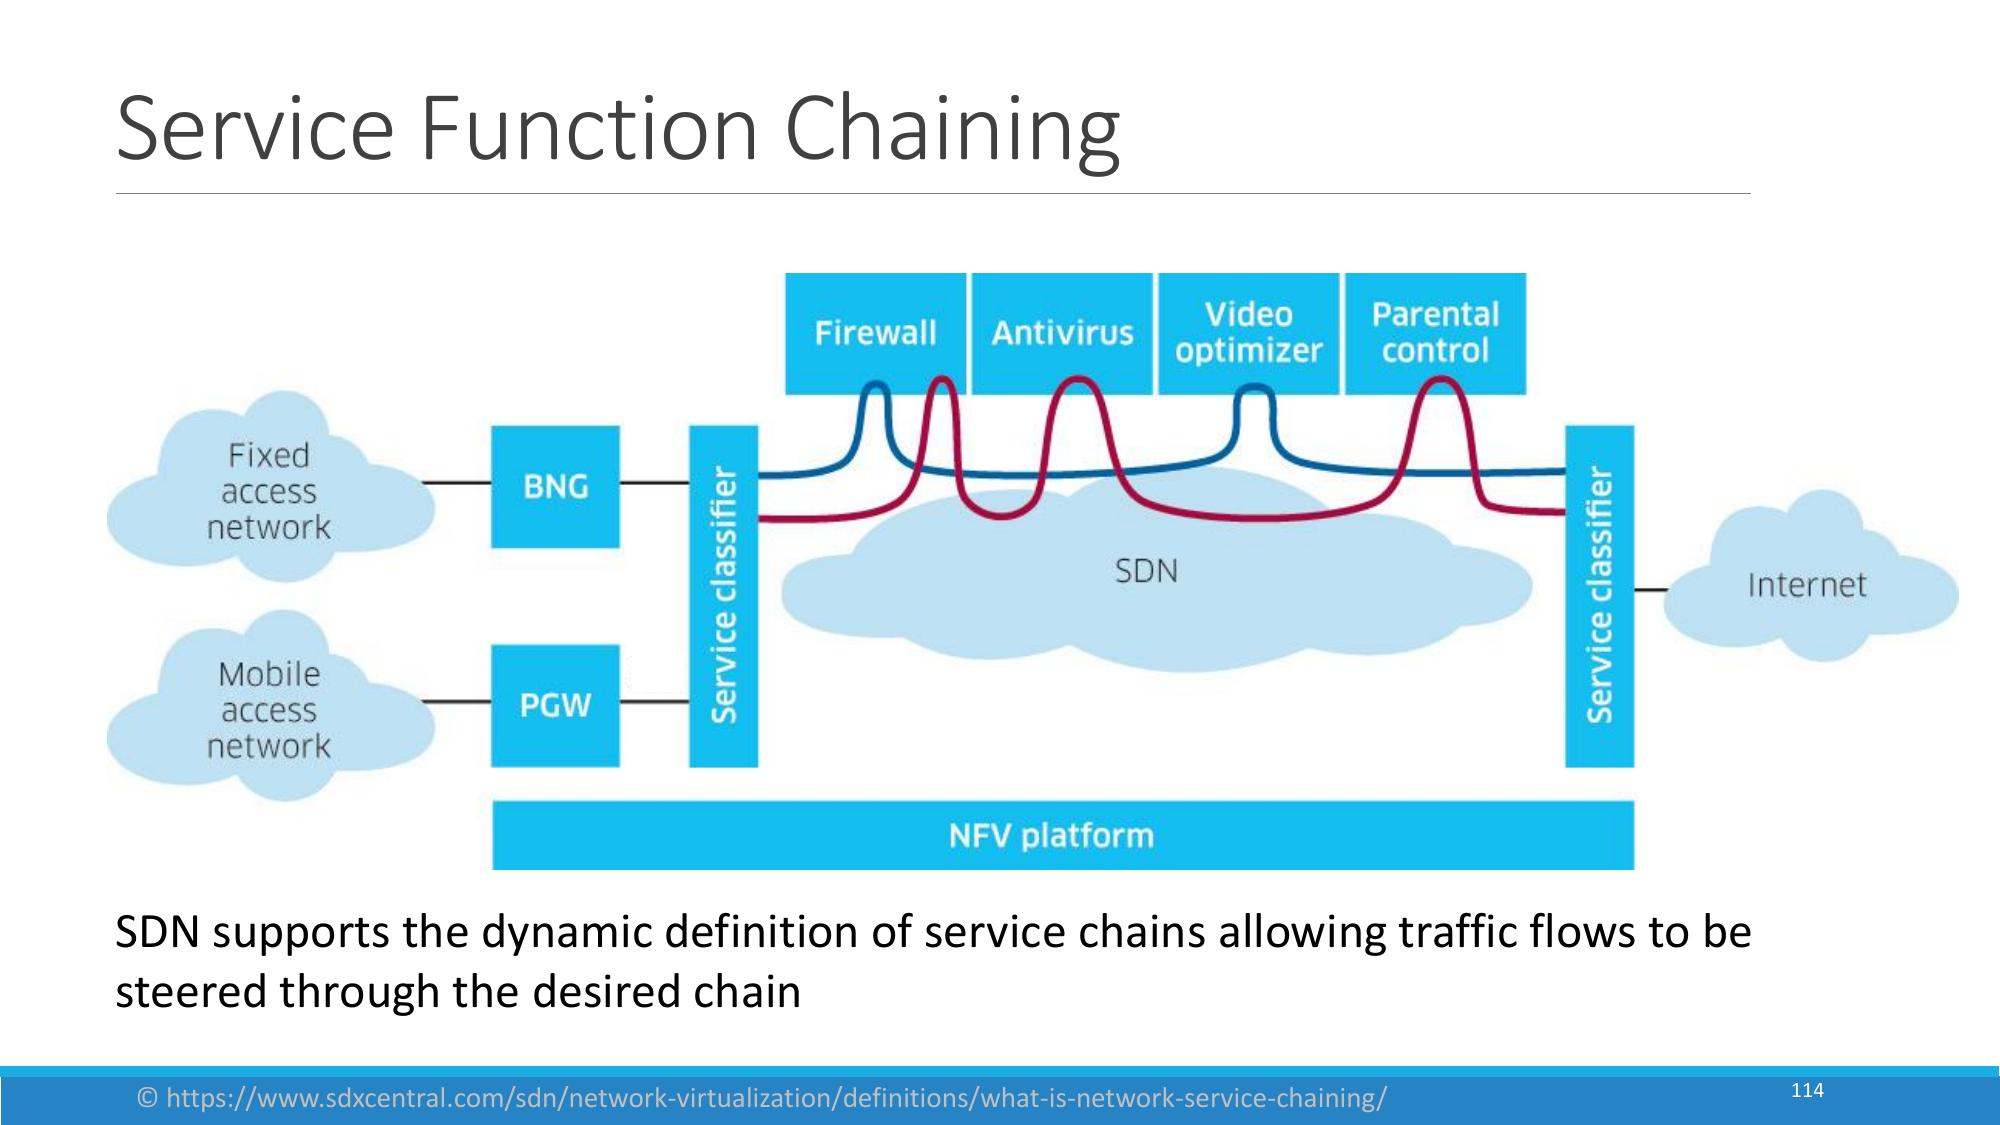
\includegraphics[keepaspectratio]{images/lezione-16-lab-sdn-applications-e-p4-language-img-11.jpg}}
\caption{SDN permette la definizione dinamica di service chain: il
traffico viene instradato dal Service Classifier attraverso le funzioni
desiderate (Firewall, Antivirus, Video Optimizer, Parental Control) su
una piattaforma NFV, senza richiedere ricablaggio fisico.}
\end{figure}

SDN risolve il problema della rigidità. Con SDN, le service chain sono
\textbf{definite programmaticamente}: il controller SDN configura le
regole di forwarding affinché i pacchetti attraversino le funzioni
desiderate nell'ordine corretto, indipendentemente dalla topologia
fisica. Un \textbf{Service Classifier} identifica i flussi e li instrada
sulla chain appropriata; alla fine della chain, un secondo
classificatore rilascia il traffico verso la destinazione finale.

Questo approccio si integra naturalmente con la \textbf{Network Function
Virtualization} (NFV): le funzioni di rete non devono essere
implementate su hardware dedicato, ma possono girare come istanze
software su una piattaforma NFV. SDN + NFV insieme abilitano chain
completamente virtuali, modificabili in tempo reale senza intervento
fisico.

\begin{callouttip}{SDN + NFV: perché si completano}

NFV virtualizza le funzioni di rete (le rende software). SDN controlla
il forwarding e permette di comporre queste funzioni in catene
dinamiche. Insieme, eliminano sia la dipendenza dall'hardware dedicato
sia la rigidità topologica delle reti tradizionali.

\end{callouttip}

\begin{center}\rule{0.5\linewidth}{0.5pt}\end{center}

\section{Sintesi}\label{sintesi}

\begin{calloutnote}{Punti chiave della lezione}

Il routing tradizionale offre un controllo troppo grossolano: i pesi dei
link e il forwarding destination-based non bastano per traffic
engineering fine-grained e controllo delle policy.

\textbf{B4} dimostra che SDN consente utilizzo vicino al 100\% dei link
WAN inter-datacenter, contro il 30--40\% delle WAN tradizionali ---
abbattendo costi e complessità. L'architettura è fisicamente distribuita
ma logicamente centralizzata, con un TE Server globale che ottimizza
l'intera rete.

\textbf{OpenFlow} è uno dei possibili meccanismi southbound di SDN ---
non è SDN stesso. I suoi limiti (data plane fisso, header predefiniti)
hanno portato allo sviluppo di P4.

\textbf{P4} estende la programmabilità al data plane: non solo installa
regole, ma permette di definire il parser, le tabelle, le azioni e il
deparser. Il risultato è un data plane completamente personalizzabile,
compilato per hardware diversi tramite un compilatore vendor-specifico.

\textbf{Service Function Chaining} con SDN permette di comporre funzioni
di rete (firewall, IDS, load balancer\ldots) in catene dinamiche, senza
ricablaggio fisico --- specialmente potente in combinazione con NFV.

\end{calloutnote}

\newpage

\chapter{Network Function
Virtualization}\label{network-function-virtualization}

La \textbf{Network Function Virtualization} (NFV) rappresenta uno dei
cambiamenti di paradigma più significativi nell'ingegneria delle reti
degli ultimi anni. L'idea fondamentale è semplice ma rivoluzionaria:
spostare le funzioni di rete --- firewall, bilanciatori di carico,
gateway --- dall'hardware proprietario dedicato a software eseguito su
infrastruttura virtualizzata generica. Questa lezione ripercorre il
problema che NFV risolve, i suoi benefici, la sua architettura e come i
servizi di rete vengono effettivamente composti e distribuiti.

\begin{center}\rule{0.5\linewidth}{0.5pt}\end{center}

\section{Il problema: middlebox e rigidità
hardware}\label{il-problema-middlebox-e-rigidituxe0-hardware}

\subsection{Un mondo di middlebox}\label{un-mondo-di-middlebox}

Le reti tradizionali non sono composte solo da router e switch. Accanto
a questi elementi ``trasparenti'' proliferano i \textbf{middlebox}:
dispositivi che eseguono funzioni di elaborazione avanzata oltre al
semplice inoltro dei pacchetti. Firewall, sistemi di rilevamento delle
intrusioni (NIDS), media gateway, load balancer, proxy, VPN gateway, WAN
optimizer --- in una grande impresa con oltre 80.000 utenti su decine di
siti, questi apparati possono essere addirittura più numerosi dei router
tradizionali.

\begin{callouttip}{Dati da una grande enterprise (Sekar et al., 2011)}

{\def\LTcaptype{none} % do not increment counter
\begin{longtable}[]{@{}ll@{}}
\toprule\noalign{}
Tipo di apparato & Numero \\
\midrule\noalign{}
\endhead
\bottomrule\noalign{}
\endlastfoot
Firewall & 166 \\
NIDS & 127 \\
Media gateway & 110 \\
Load balancer & 67 \\
Proxy & 66 \\
VPN gateway & 45 \\
WAN Optimizer & 44 \\
\textbf{Totale middlebox} & \textbf{636} \\
Totale router & \textasciitilde900 \\
\end{longtable}
}

I middlebox sono quasi pari in numero ai router: la rete è molto più di
semplice forwarding.

\end{callouttip}

\subsection{Il modello tradizionale e i suoi
limiti}\label{il-modello-tradizionale-e-i-suoi-limiti}

Nell'industria delle telecomunicazioni tradizionale, ogni funzione di
rete corrisponde a un \textbf{apparato hardware proprietario} dedicato.
Il firewall è un box fisico, il load balancer è un altro box fisico, e
così via. Questo modello impone vincoli severi:

\begin{itemize}
\tightlist
\item
  Le funzioni devono essere concatenate in un ordine preciso, riflesso
  nella topologia fisica della rete (es. il traffico deve passare prima
  per il firewall e poi per il load balancer --- non si può cambiare
  senza ricablare).
\item
  I fornitori devono garantire alti standard di qualità, performance e
  conformità ai protocolli, con cicli di sviluppo prodotto molto lunghi.
\item
  Il risultato è una \textbf{scarsa agilità}: aggiungere una nuova
  funzione o scalare una esistente richiede acquisto di nuovo hardware,
  deployment manuale e formazione del personale.
\end{itemize}

Contemporaneamente, gli utenti richiedono servizi sempre più
diversificati e di breve durata. Ogni nuovo servizio richiede nuovo
hardware, deployment manuale e nuove competenze. Le reti diventano
complesse, difficili da scalare e costose da operare: i costi
\textbf{CAPEX} (\emph{Capital Expenditure}, l'investimento in hardware e
infrastruttura fisica) e \textbf{OPEX} (\emph{Operational Expenditure},
i costi operativi di energia, manutenzione e personale) crescono, ma i
ricavi no.

\begin{calloutwarning}{Il nodo del problema}

Il modello hardware-based è per natura \emph{lento e rigido}. I provider
di servizi Internet (Google, Amazon, Facebook) hanno invece dimostrato
che un approccio \emph{software-based} è \emph{veloce e flessibile}. NFV
nasce dalla volontà di portare questo modello software dentro le reti di
telecomunicazione.

\end{calloutwarning}

\begin{center}\rule{0.5\linewidth}{0.5pt}\end{center}

\section{NFV: l'idea fondamentale}\label{nfv-lidea-fondamentale}

Nel 2012, i principali operatori globali (AT\&T, Telefónica, Verizon e
altri) avviarono un'iniziativa presso \textbf{ETSI} (European
Telecommunications Standards Institute), dando vita all'Industry
Specification Group for NFV. L'obiettivo: trasformare le reti attraverso
la virtualizzazione.

\subsection{Decoupling tra funzioni e
hardware}\label{decoupling-tra-funzioni-e-hardware}

Il principio cardine di NFV è il \textbf{disaccoppiamento}
(\emph{decoupling}) tra le funzioni di rete e l'hardware su cui girano.
Le funzioni non sono più implementate in appliance fisiche dedicate, ma
come \textbf{software} eseguito su infrastruttura virtualizzata standard
(macchine virtuali o container su server COTS --- \emph{Commercial
Off-The-Shelf}).

\begin{figure}
\centering
\pandocbounded{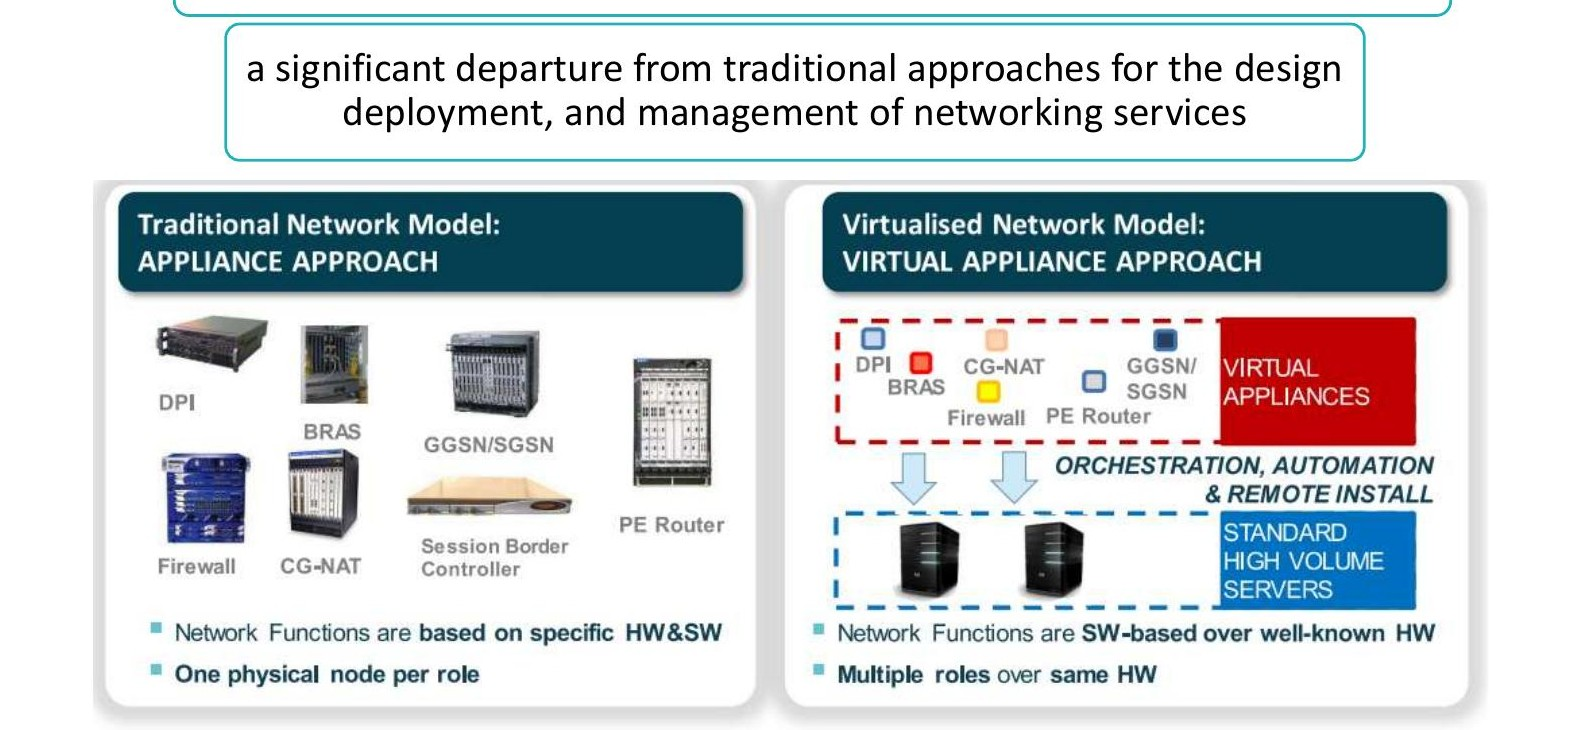
\includegraphics[keepaspectratio]{images/lezione-20-lab-network-function-virtualization-img-01.jpg}}
\caption{A sinistra, il modello tradizionale: ogni funzione (DPI,
Firewall, BRAS, CG-NAT\ldots) richiede HW specifico e un solo ruolo per
nodo. A destra, il modello NFV: le stesse funzioni girano come software
su server standard ad alto volume, orchestrate in modo automatico e
remoto.}
\end{figure}

Nel modello tradizionale le funzioni di rete sono basate su HW e SW
proprietari, con un nodo fisico per ogni ruolo. Nel modello NFV le
funzioni sono implementate in software su hardware commodity, e più
ruoli possono coesistere sullo stesso server fisico.

\begin{center}\rule{0.5\linewidth}{0.5pt}\end{center}

\section{Vantaggi di NFV}\label{vantaggi-di-nfv}

NFV introduce tre famiglie di benefici fondamentali:

\textbf{Flessibilità}: le funzioni possono essere deployate ovunque
nell'infrastruttura e spostate dinamicamente in base alle esigenze,
grazie all'allocazione flessibile delle risorse hardware condivise
(\emph{hardware pool}).

\textbf{Scalabilità ed efficienza}: la capacità dedicata a ciascuna
funzione può essere modificata dinamicamente (\emph{scaling up/down}) in
base al carico effettivo, migliorando l'utilizzo delle risorse. Non è
più necessario acquistare hardware ridondante per gestire i picchi: si
alloca più capacità software quando serve e la si riduce quando non
serve.

\textbf{Innovazione accelerata}: il ciclo di sviluppo di un nuovo
servizio di rete si accorcia drasticamente, perché non richiede
procurement hardware ma soltanto deployment software.

\begin{calloutnote}{NFV introduce anche nuove sfide}

La virtualizzazione porta con sé problemi nuovi: gestione del ciclo di
vita delle funzioni, orchestrazione, performance (overhead della
virtualizzazione), sicurezza dell'infrastruttura condivisa, e il
complesso problema del \emph{placement} delle funzioni virtualizzate.

\end{calloutnote}

\begin{center}\rule{0.5\linewidth}{0.5pt}\end{center}

\section{Da funzioni di rete a servizi di
rete}\label{da-funzioni-di-rete-a-servizi-di-rete}

\subsection{Composizione di funzioni}\label{composizione-di-funzioni}

Una singola funzione (es. un firewall) non è sufficiente a realizzare un
servizio reale. I servizi richiedono la \textbf{composizione di più
funzioni} applicate in sequenza al traffico. In un servizio tipico, un
utente che accede a Internet deve attraversare: firewall → antivirus →
video optimizer → parental control. Sequenze diverse possono applicarsi
a traffici diversi.

\begin{figure}
\centering
\pandocbounded{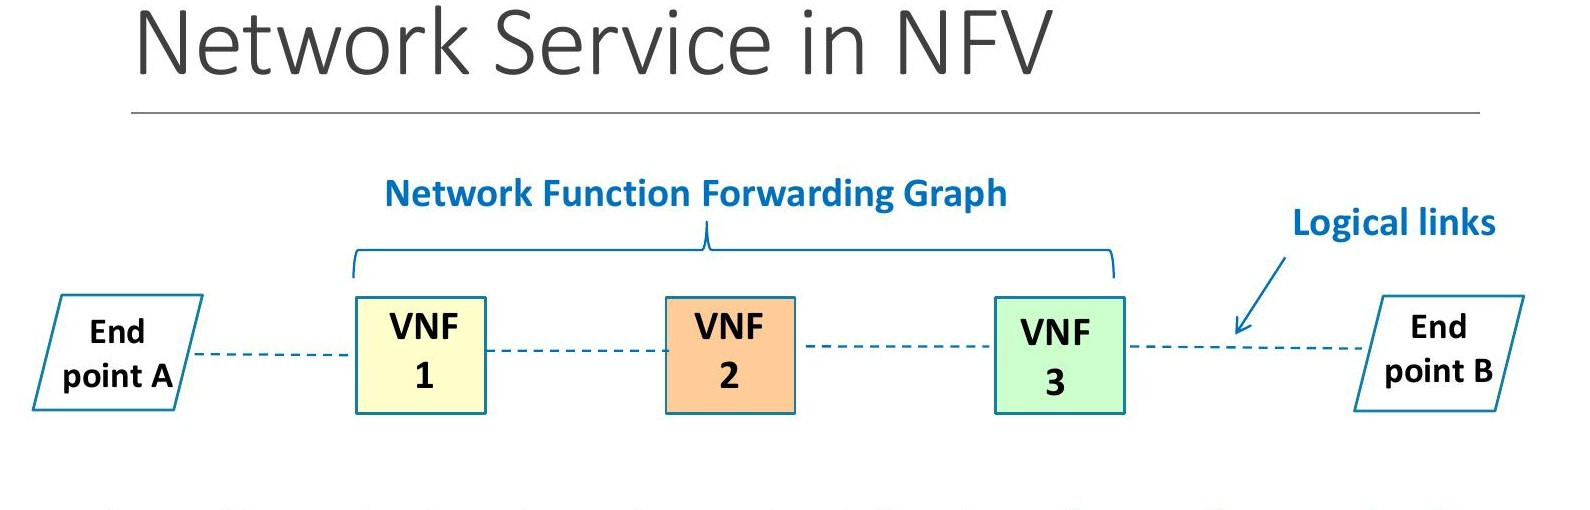
\includegraphics[keepaspectratio]{images/lezione-20-lab-network-function-virtualization-img-02.jpg}}
\caption{Un servizio di rete minimo: il traffico dell'utente attraversa
in sequenza Firewall, NAT e Load Balancer prima di raggiungere il Web
Service.}
\end{figure}

In un'infrastruttura reale, non tutto il traffico segue la stessa
catena: il servizio non è una pipeline fissa ma una composizione
flessibile di funzioni, dipendente dai requisiti del flusso. Questo pone
la domanda: come modificare le rotte per applicare trattamenti
differenziati a flussi diversi? La risposta è {[}{[}Software Defined
Networking{]}{]} (SDN), che fornisce il piano di controllo per il
service chaining.

\begin{figure}
\centering
\pandocbounded{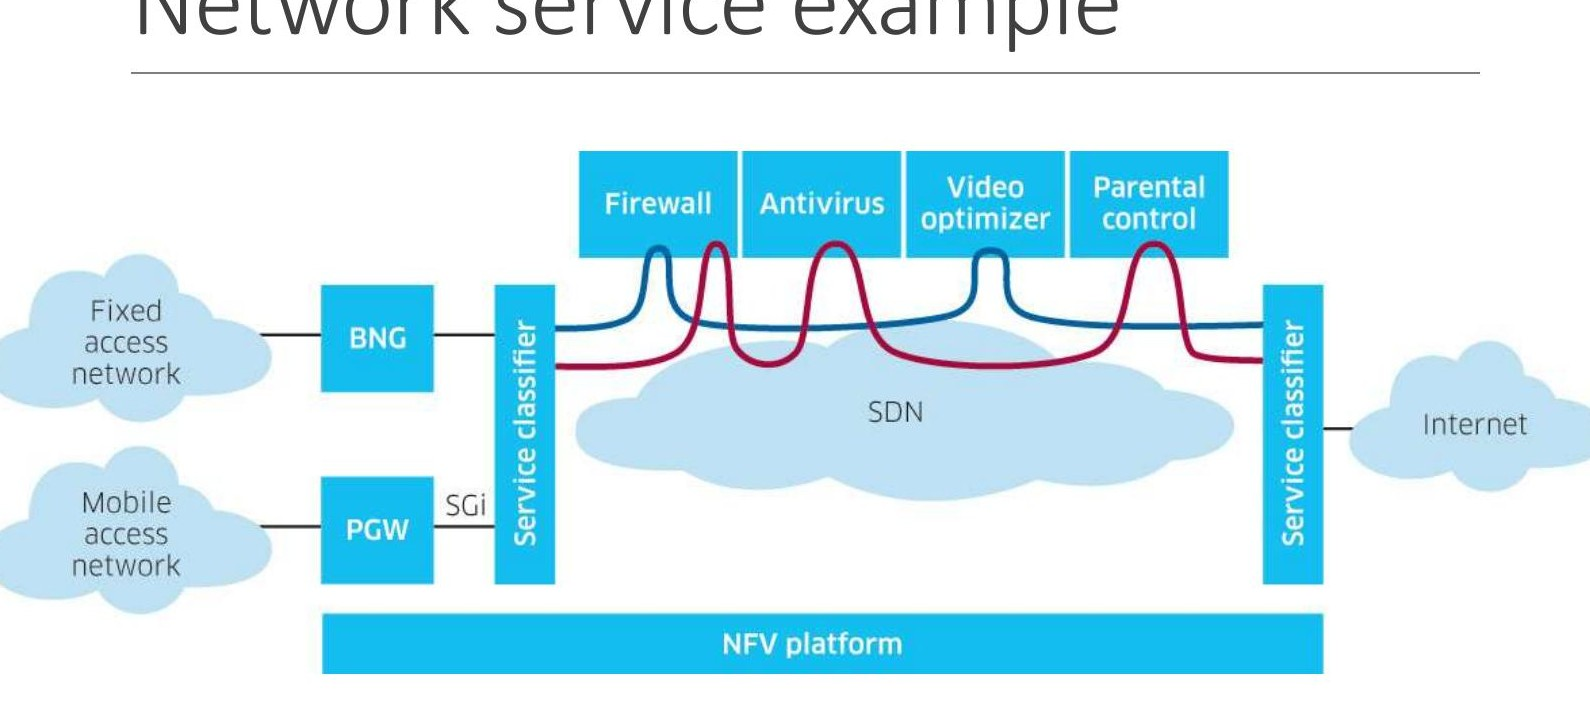
\includegraphics[keepaspectratio]{images/lezione-20-lab-network-function-virtualization-img-03.jpg}}
\caption{Le reti fissa e mobile convergono su una piattaforma NFV. Un
service classifier instrada il traffico attraverso funzioni diverse
(Firewall, Antivirus, Video optimizer, Parental control) via SDN, prima
di raggiungere Internet.}
\end{figure}

\subsection{Network Function Forwarding Graph
(NF-FG)}\label{network-function-forwarding-graph-nf-fg}

In NFV, un servizio di rete end-to-end è formalizzato come un
\textbf{grafo di forwarding} di funzioni di rete e punti terminali.
Questo è ciò che un operatore fornisce ai propri clienti.

\begin{figure}
\centering
\pandocbounded{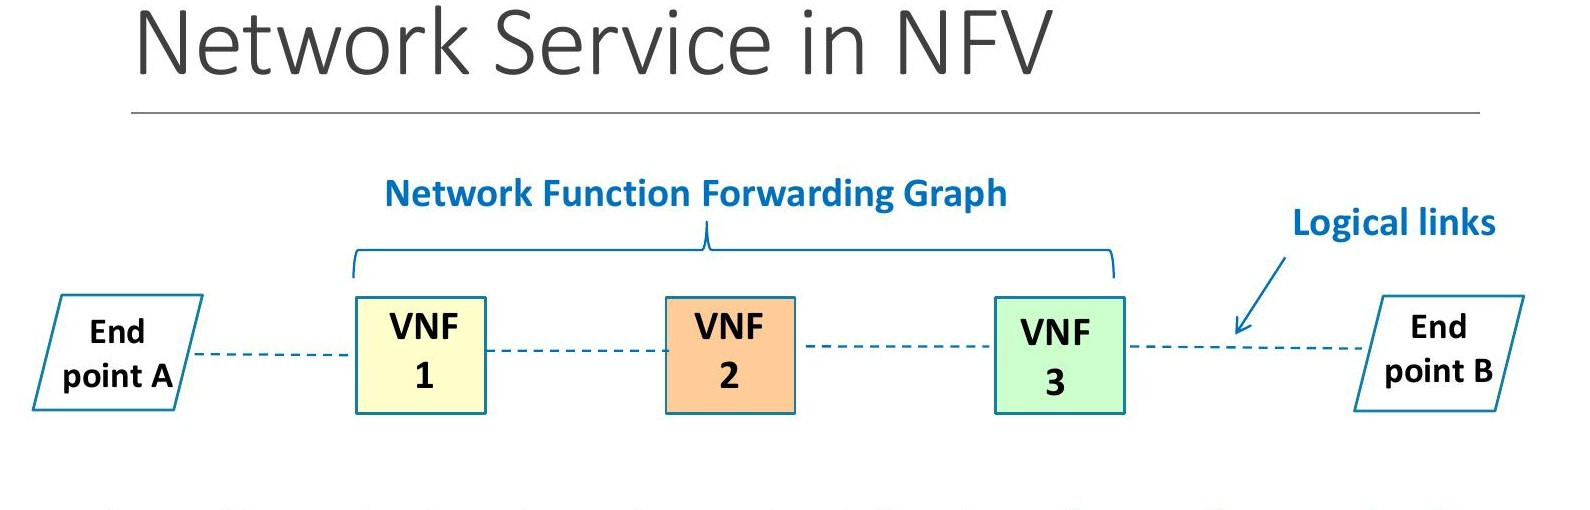
\includegraphics[keepaspectratio]{images/lezione-20-lab-network-function-virtualization-img-04.jpg}}
\caption{Un servizio end-to-end è un grafo: l'endpoint A è connesso
all'endpoint B attraverso VNF 1, VNF 2 e VNF 3 via link logici.}
\end{figure}

\begin{calloutdefinition}{VNF — Virtualized Network Function}

Una \textbf{Virtualized Network Function} (VNF) è l'implementazione
software di una funzione di rete tradizionalmente realizzata in hardware
dedicato (firewall, load balancer, NAT, ecc.), eseguita su risorse
virtualizzate (VM o container).

\end{calloutdefinition}

La separazione fondamentale introdotta da NF-FG è tra: - la
\textbf{definizione logica del servizio}: il grafo descrive quali
funzioni servono e come sono connesse (link logici) - il
\textbf{deployment fisico}: i link logici sono supportati da percorsi
fisici attraverso reti di infrastruttura distinte

\begin{figure}
\centering
\pandocbounded{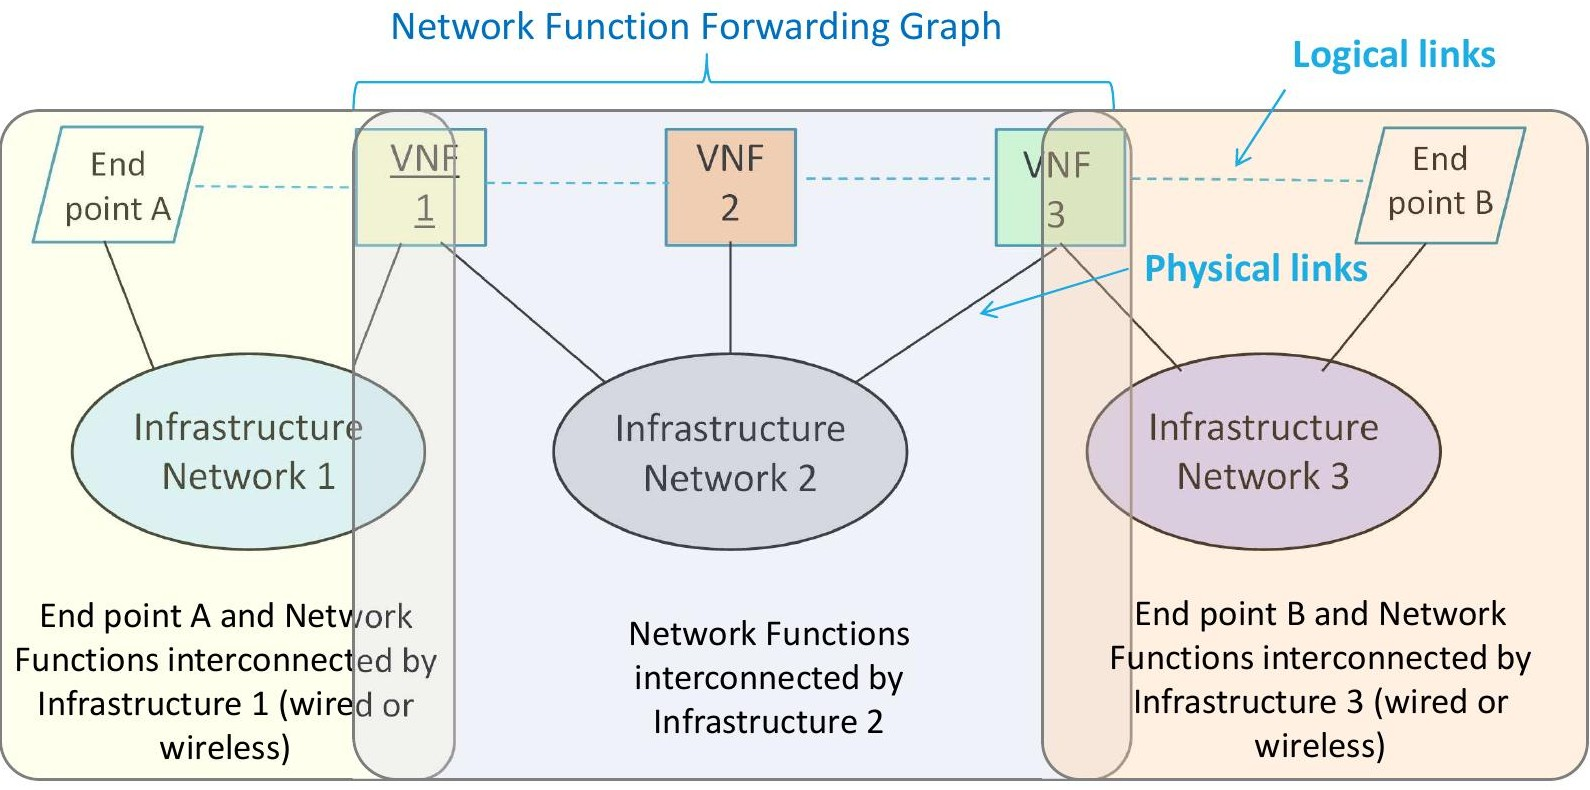
\includegraphics[keepaspectratio]{images/lezione-20-lab-network-function-virtualization-img-05.jpg}}
\caption{Il grafo logico del servizio (VNF 1, VNF 2, VNF 3 con link
tratteggiati) è mappato su tre reti di infrastruttura fisiche distinte.
La separazione logico/fisico è il principio chiave.}
\end{figure}

\subsection{VNF-FG nidificati e PoP}\label{vnf-fg-nidificati-e-pop}

Le VNF girano su nodi fisici chiamati \textbf{PoP} (\emph{Points of
Presence}). I grafi di forwarding possono essere nidificati: un VNF-FG
può essere costruito componendo altri VNF-FG (esempio: VNF-FG-2 composto
da VNF-2A, VNF-2B e VNF-2C), consentendo la definizione di servizi
gerarchici e riutilizzabili.

\begin{figure}
\centering
\pandocbounded{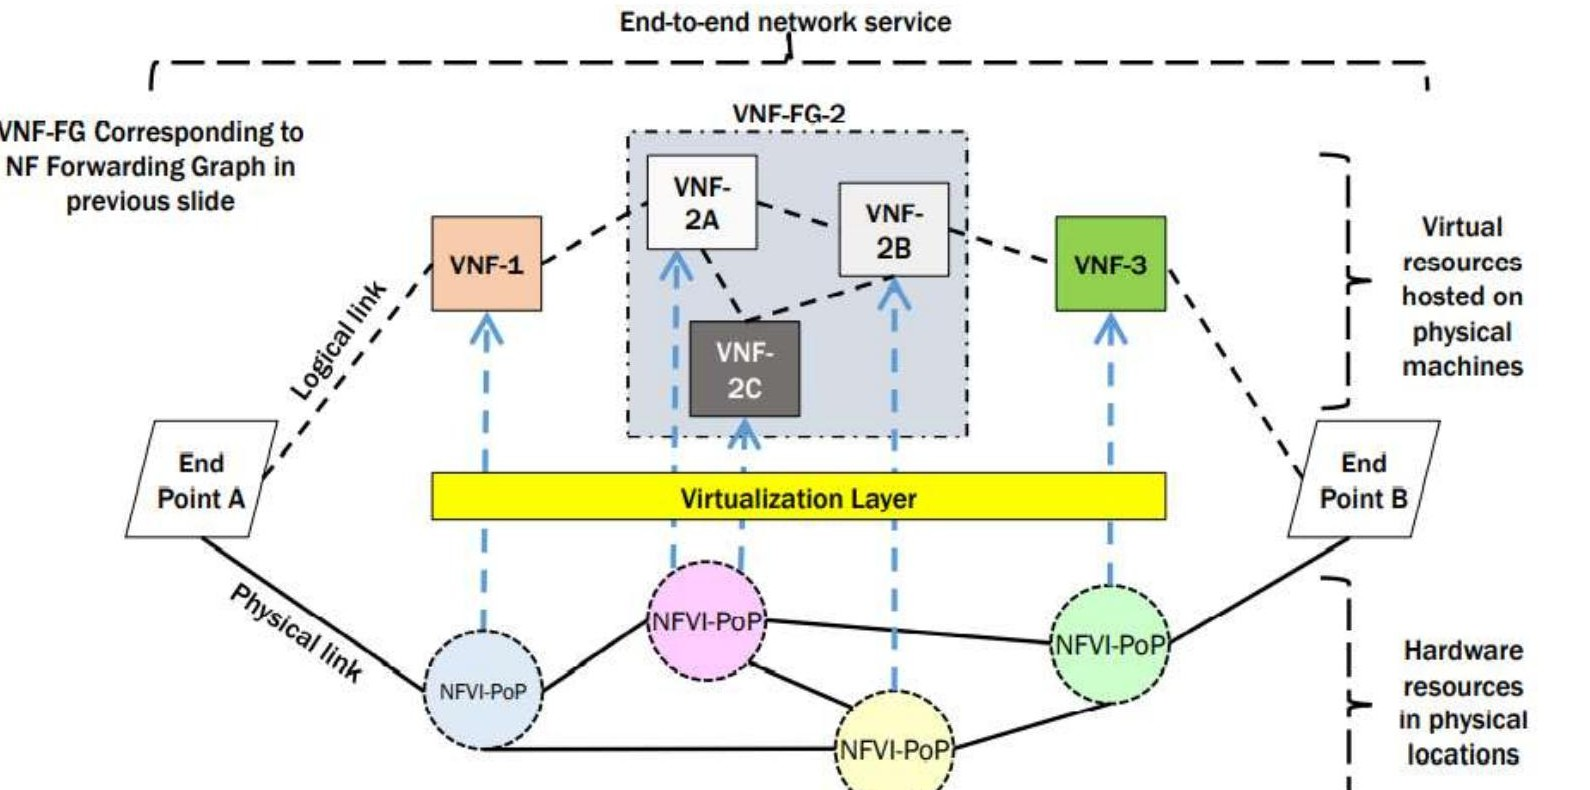
\includegraphics[keepaspectratio]{images/lezione-20-lab-network-function-virtualization-img-06.jpg}}
\caption{Il servizio end-to-end (tra End Point A e B) è un VNF-FG
composto da VNF-1, dal sotto-grafo VNF-FG-2 (con VNF-2A, VNF-2B, VNF-2C)
e VNF-3. Le VNF girano su PoP fisici (NFVI-PoP) tramite un livello di
virtualizzazione.}
\end{figure}

\begin{center}\rule{0.5\linewidth}{0.5pt}\end{center}

\section{Il problema del VNF
Placement}\label{il-problema-del-vnf-placement}

Dato un servizio di rete composto da più VNF, occorre decidere
\textbf{dove deployare ciascuna funzione} nell'infrastruttura fisica.
Questo è il problema del \emph{VNF chain placement}, uno dei problemi di
ottimizzazione centrali in NFV.

Gli obiettivi di ottimizzazione tipici sono: - minimizzare la latenza
end-to-end - minimizzare i costi di deployment - massimizzare la banda
residua - risparmiare energia

Soggetti ai vincoli di: - capacità computazionale dei nodi - banda
disponibile sui link - requisiti di QoS (latenza massima, banda minima)

\begin{callouttip}{VNF placement e 5G Network Slicing}

Il VNF placement è particolarmente rilevante nel contesto del
{[}{[}5G{]}{]} e del \textbf{network slicing}: ogni slice deve avere una
catena di VNF dedicata con garanzie di isolamento e QoS. L'orchestratore
deve risolvere il problema di placement per ogni slice
contemporaneamente, spesso con obiettivi conflittuali.

\end{callouttip}

Gli approcci risolutivi spaziano dalla \textbf{programmazione
matematica} (ILP, MILP) alle \textbf{euristiche} e
\textbf{metaeuristiche} (Algoritmi Genetici), fino al \textbf{Deep
Reinforcement Learning} per scenari dinamici.

\subsection{Nuove sfide: hardware
programmabile}\label{nuove-sfide-hardware-programmabile}

Le VNF possono essere deployate non solo su server, ma anche su
\textbf{dispositivi di rete programmabili}, ciascuno con un profilo
prestazionale diverso:

{\def\LTcaptype{none} % do not increment counter
\begin{longtable}[]{@{}
  >{\raggedright\arraybackslash}p{(\linewidth - 4\tabcolsep) * \real{0.3333}}
  >{\raggedright\arraybackslash}p{(\linewidth - 4\tabcolsep) * \real{0.3333}}
  >{\raggedright\arraybackslash}p{(\linewidth - 4\tabcolsep) * \real{0.3333}}@{}}
\toprule\noalign{}
\begin{minipage}[b]{\linewidth}\raggedright
Dispositivo
\end{minipage} & \begin{minipage}[b]{\linewidth}\raggedright
Latenza per pacchetto
\end{minipage} & \begin{minipage}[b]{\linewidth}\raggedright
Caratteristiche
\end{minipage} \\
\midrule\noalign{}
\endhead
\bottomrule\noalign{}
\endlastfoot
Programmable switch & 1--2 µs & Velocissimo, ma memoria e flessibilità
limitate \\
Server (COTS) & 1--10 µs & Flessibile, ma più lento \\
SmartNIC & 10--100+ µs & Soluzione intermedia \\
\end{longtable}
}

La scelta del dispositivo su cui deployare ciascuna VNF aggiunge una
dimensione ulteriore al problema di placement.

\begin{center}\rule{0.5\linewidth}{0.5pt}\end{center}

\section{L'architettura NFV}\label{larchitettura-nfv}

L'architettura di riferimento NFV, standardizzata da ETSI, è organizzata
in tre blocchi principali: l'\textbf{infrastruttura} (NFVI), le
\textbf{funzioni virtualizzate} (VNF) e il \textbf{sistema di gestione e
orchestrazione} (NFV-MANO).

\begin{figure}
\centering
\pandocbounded{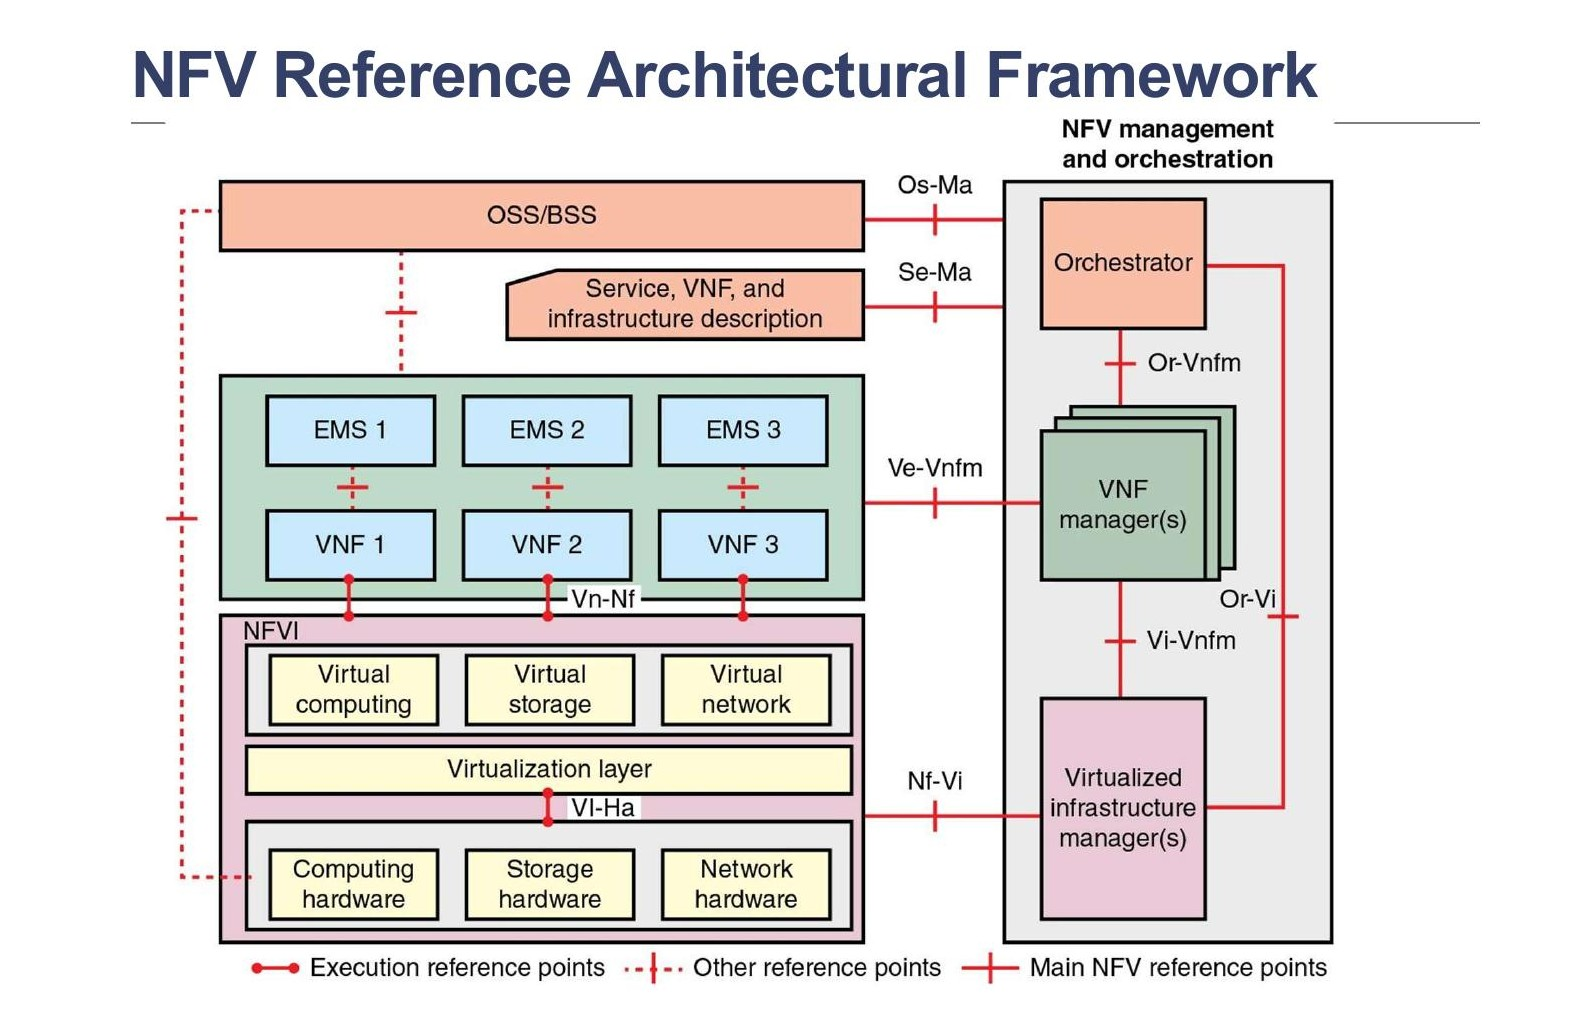
\includegraphics[keepaspectratio]{images/lezione-20-lab-network-function-virtualization-img-07.jpg}}
\caption{Il framework architetturale di riferimento NFV secondo
ETSI/Stallings. Le frecce indicano i reference point: Or-Vi, Or-Vnfm,
Ve-Vnfm, Vi-Vnfm, Nf-Vi, Se-Ma, Os-Ma.}
\end{figure}

\subsection{NFV Infrastructure (NFVI)}\label{nfv-infrastructure-nfvi}

L'\textbf{NFVI} è la totalità delle risorse hardware e software che
costituiscono l'ambiente di esecuzione delle VNF. Virtualizza risorse
fisiche di computing, storage e networking raggruppandole in
\emph{resource pool}.

È composta da tre domini:

\begin{itemize}
\tightlist
\item
  \textbf{Compute domain}: fornisce server COTS ad alto volume e
  storage.
\item
  \textbf{Hypervisor domain}: media le risorse del compute domain alle
  VM (o container) delle VNF, fornendo un'astrazione dell'hardware. Oggi
  le VNF sono spesso eseguite in container → \textbf{Cloud Native
  Functions (CNF)}.
\item
  \textbf{Infrastructure network domain}: switch generici ad alto volume
  interconnessi in una rete configurabile per erogare servizi di rete.
\end{itemize}

\begin{figure}
\centering
\pandocbounded{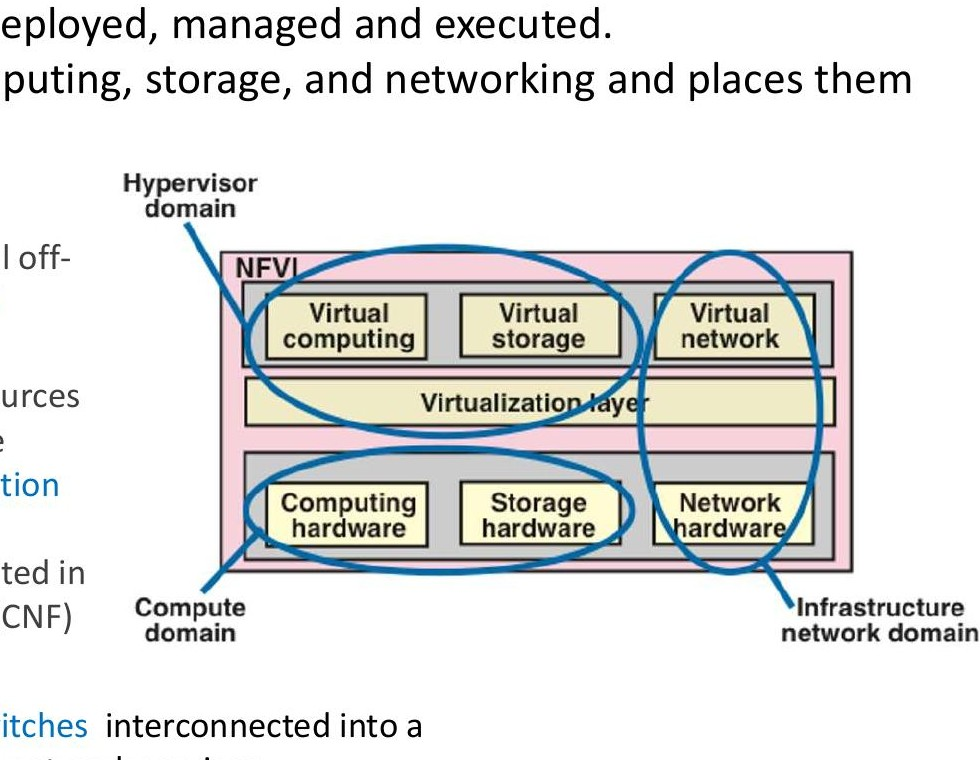
\includegraphics[keepaspectratio]{images/lezione-20-lab-network-function-virtualization-img-08.jpg}}
\caption{L'NFVI si stratifica in tre livelli: hardware fisico (compute,
storage, network hardware), virtualizzazione (hypervisor/virtualization
layer) e risorse virtuali (virtual computing, storage, network).}
\end{figure}

L'NFVI può distribuirsi su più \textbf{NFVI-PoP} (\emph{Network Function
Virtualization Infrastructure Point of Presence}): posizioni fisiche
dove sono deployate le risorse di infrastruttura NFV. Due tipi di rete
interconnettono i PoP: - \textbf{NFVI-PoP network}: connette le risorse
all'interno di un PoP. - \textbf{Transport network}: interconnette i
vari NFVI-PoP tra loro e verso l'esterno.

\subsubsection{vSwitch}\label{vswitch}

All'interno di un PoP, le VM sono collegate a interfacce virtuali
(\textbf{VIF}). Un \textbf{virtual switch} (vSwitch) è un programma
software che emula uno switch di livello 2, fornendo connettività tra le
VIF e le interfacce fisiche (PIF), oltre a gestire il traffico tra VIF
sullo stesso host fisico. L'esempio più noto è \textbf{Open vSwitch}
(OVS), che supporta OpenFlow e può integrarsi con switch fisici.

\subsubsection{Opzioni di
virtualizzazione}\label{opzioni-di-virtualizzazione}

Le VNF possono essere eseguite in \textbf{macchine virtuali} (VM) o in
\textbf{container}. La differenza fondamentale:

\begin{figure}
\centering
\pandocbounded{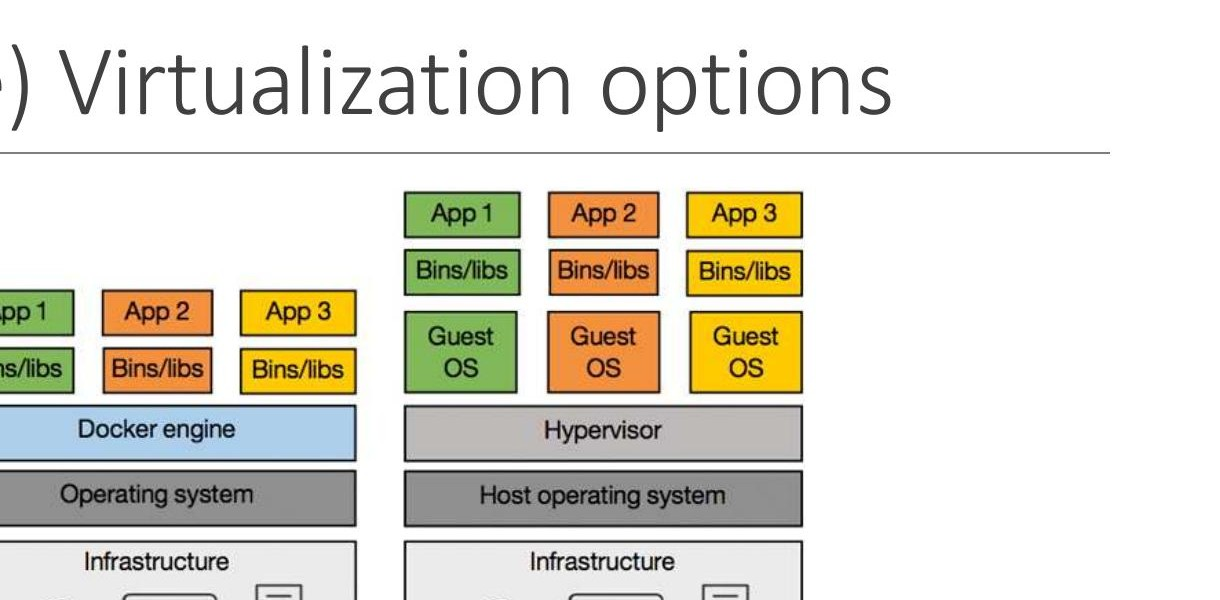
\includegraphics[keepaspectratio]{images/lezione-20-lab-network-function-virtualization-img-09.jpg}}
\caption{A sinistra i container: condividono il kernel dell'host,
isolati in userspace tramite Docker engine. A destra le VM: includono un
guest OS completo sopra l'hypervisor.}
\end{figure}

\begin{calloutdefinition}{Container vs VM}

I \textbf{container} includono l'applicazione e le sue dipendenze ma
condividono il kernel dell'host OS, girando come processi isolati in
userspace. Le \textbf{VM} includono invece l'applicazione, le librerie
necessarie e un intero guest OS, con un overhead maggiore ma un
isolamento più forte.

\end{calloutdefinition}

\subsection{NFV Management and Orchestration
(NFV-MANO)}\label{nfv-management-and-orchestration-nfv-mano}

Il \textbf{MANO} è il framework che gestisce e orchestra tutte le
risorse nell'ambiente NFV. Comprende:

\subsubsection{NFV Orchestrator (NFVO)}\label{nfv-orchestrator-nfvo}

Responsabile di installare e configurare nuovi \textbf{Network Service
(NS)} e pacchetti VNF, gestire il ciclo di vita dei servizi di rete e le
risorse globali. Opera su due piani: - \textbf{Network services
orchestration}: gestisce/coordina la creazione di servizi end-to-end tra
VNF diverse, può istanziare nuovi VNFM. - Esempi di implementazioni open
source: \textbf{OSM MANO} (ETSI) e \textbf{ONAP} (Linux Foundation).

\subsubsection{VNF Manager (VNFM)}\label{vnf-manager-vnfm}

Gestisce il \textbf{ciclo di vita delle istanze VNF}: - istanziazione
(con configurazione iniziale se richiesta dal deployment template) -
scaling out/in e up/down - raccolta di misure di performance dell'NFVI e
correlazione con eventi/fault VNF - healing automatico o assistito -
terminazione dell'istanza

\subsubsection{Virtualized Infrastructure Manager
(VIM)}\label{virtualized-infrastructure-manager-vim}

Il \textbf{VIM} controlla e gestisce l'interazione delle VNF con le
risorse fisiche (computing, storage, network) e la loro
virtualizzazione, tipicamente all'interno del dominio infrastrutturale
di un singolo operatore. Piattaforme IaaS come \textbf{OpenStack}
fungono da VIM. Un MANO può orchestrare più VIM.

\subsection{Repository MANO}\label{repository-mano}

Il sistema MANO utilizza quattro repository:

{\def\LTcaptype{none} % do not increment counter
\begin{longtable}[]{@{}
  >{\raggedright\arraybackslash}p{(\linewidth - 2\tabcolsep) * \real{0.5000}}
  >{\raggedright\arraybackslash}p{(\linewidth - 2\tabcolsep) * \real{0.5000}}@{}}
\toprule\noalign{}
\begin{minipage}[b]{\linewidth}\raggedright
Repository
\end{minipage} & \begin{minipage}[b]{\linewidth}\raggedright
Contenuto
\end{minipage} \\
\midrule\noalign{}
\endhead
\bottomrule\noalign{}
\endlastfoot
\textbf{Network services catalog} & Template di deployment dei network
service in termini di VNF e virtual link \\
\textbf{VNF catalog} & VNF Descriptor (VNFD): descrive deployment e
behavior di ogni VNF \\
\textbf{NFVI resources} & Lista delle risorse NFVI utilizzate per i
servizi NFV attivi \\
\textbf{NFV instances} & Dettagli sulle istanze di network service e VNF
in esecuzione \\
\end{longtable}
}

\begin{center}\rule{0.5\linewidth}{0.5pt}\end{center}

\section{Network Service Descriptor: un
esempio}\label{network-service-descriptor-un-esempio}

Il deployment di un network service è descritto tramite un
\textbf{Network Service Descriptor (NSD)}, un documento strutturato
(tipicamente JSON/YAML) che specifica la composizione del servizio.

\begin{callouttip}{NSD per un servizio iperf (client-server)}

\begin{Shaded}
\begin{Highlighting}[]
\FunctionTok{\{}
  \DataTypeTok{"name"}\FunctionTok{:} \StringTok{"iperf{-}NSD"}\FunctionTok{,}
  \DataTypeTok{"vendor"}\FunctionTok{:} \StringTok{"fokus"}\FunctionTok{,}
  \DataTypeTok{"version"}\FunctionTok{:} \StringTok{"0.1{-}ALPHA"}\FunctionTok{,}
  \DataTypeTok{"vnfd"}\FunctionTok{:} \OtherTok{[} \ErrorTok{...} \OtherTok{]}\FunctionTok{,}
  \DataTypeTok{"vld"}\FunctionTok{:} \OtherTok{[} \FunctionTok{\{} \DataTypeTok{"name"}\FunctionTok{:} \StringTok{"private"} \FunctionTok{\}} \OtherTok{]}\FunctionTok{,}
  \DataTypeTok{"vnf\_dependency"}\FunctionTok{:} \OtherTok{[}
    \FunctionTok{\{}
      \DataTypeTok{"source"}\FunctionTok{:} \FunctionTok{\{} \DataTypeTok{"name"}\FunctionTok{:} \StringTok{"iperf{-}server"} \FunctionTok{\},}
      \DataTypeTok{"target"}\FunctionTok{:} \FunctionTok{\{} \DataTypeTok{"name"}\FunctionTok{:} \StringTok{"iperf{-}client"} \FunctionTok{\},}
      \DataTypeTok{"parameters"}\FunctionTok{:} \OtherTok{[}\StringTok{"private"}\OtherTok{]}
    \FunctionTok{\}}
  \OtherTok{]}
\FunctionTok{\}}
\end{Highlighting}
\end{Shaded}

{\def\LTcaptype{none} % do not increment counter
\begin{longtable}[]{@{}
  >{\raggedright\arraybackslash}p{(\linewidth - 2\tabcolsep) * \real{0.5000}}
  >{\raggedright\arraybackslash}p{(\linewidth - 2\tabcolsep) * \real{0.5000}}@{}}
\toprule\noalign{}
\begin{minipage}[b]{\linewidth}\raggedright
Campo
\end{minipage} & \begin{minipage}[b]{\linewidth}\raggedright
Significato
\end{minipage} \\
\midrule\noalign{}
\endhead
\bottomrule\noalign{}
\endlastfoot
\texttt{name} & Nome del Network Service \\
\texttt{vendor} & Provider del servizio \\
\texttt{vnfd} & Lista delle VNF che compongono il servizio \\
\texttt{vld} & Virtual Link: connettività tra VNF \\
\texttt{vnf\_dependency} & Dipendenza tra VNF: l'iperf-server deve
fornire il proprio IP all'iperf-client \\
\end{longtable}
}

\end{callouttip}

Il VNFD per ogni VNF specifica: immagine VM, risorse (flavour), virtual
link, lifecycle events (script da eseguire all'istanziazione:
\texttt{install.sh}, \texttt{start-srv.sh}) e configurazione.

\begin{center}\rule{0.5\linewidth}{0.5pt}\end{center}

\section{Casi d'uso}\label{casi-duso}

NFV è applicabile sia alle funzioni del \textbf{piano dati} che a quelle
del \textbf{piano di controllo} nelle reti mobili e fisse:

\begin{itemize}
\tightlist
\item
  \textbf{Traffic analysis}: DPI (\emph{Deep Packet Inspection}),
  misurazione QoE
\item
  \textbf{Application-level optimization}: cache server, load balancer,
  application accelerator
\item
  \textbf{Sicurezza}: firewall, virus scanner, IDS, spam protection,
  gateway IPsec/SSL VPN
\item
  \textbf{Nodi di rete mobile}: HLR/HSS, MME, SGSN, PDN-GW, eNodeB (sia
  il core EPC che la RAN possono essere in larga parte virtualizzati)
\item
  \textbf{Infrastruttura di rete}: broadband gateway, CG-NAT, router
\item
  \textbf{Edge \& Home}: home router, set-top box
\item
  \textbf{Controllo \& Gestione}: AAA server, policy control, sistemi di
  charging
\end{itemize}

\begin{center}\rule{0.5\linewidth}{0.5pt}\end{center}

\section{Sintesi}\label{sintesi-1}

\begin{calloutnote}{NFV in sintesi}

Nelle reti tradizionali, ogni dispositivo è deployato su piattaforme
proprietarie/chiuse. Gli elementi di rete sono box chiusi, l'hardware
non può essere condiviso, e ogni device richiede hardware aggiuntivo per
aumentare la capacità --- hardware che rimane inattivo quando il sistema
è sotto carico.

Con NFV, gli elementi di rete sono \textbf{applicazioni indipendenti}
deployate in modo flessibile su una piattaforma unificata di server
standard, storage e switch commodity. Software e hardware sono
disaccoppiati, e la capacità per ogni applicazione viene aumentata o
ridotta aggiungendo o riducendo risorse virtuali.

I benefici principali: \textbf{flessibilità}, \textbf{innovazione più
rapida}, possibilità di \textbf{scalare i servizi rapidamente} su/giù
secondo le necessità.

\end{calloutnote}

\newpage

\chapter{Lezione 21 --- (Lab) Network Emulator con
ComNetsEmu}\label{lezione-21-lab-network-emulator-con-comnetsemu}

\section{Laboratorio: Network Emulator con
ComNetsEmu}\label{laboratorio-network-emulator-con-comnetsemu}

Questa lezione di laboratorio introduce \textbf{ComNetsEmu}, un
emulatore di reti progettato per sperimentare ambienti {[}{[}SDN{]}{]}
({[}{[}Software-Defined Networking{]}{]}) e {[}{[}NFV{]}{]}
({[}\hyperref[network-function-virtualization]{Network Function
Virtualization}{]}) su un singolo computer. Prima di avviare gli
esperimenti è necessario installare e configurare l'ambiente: questa
guida accompagna passo per passo dall'installazione fino all'esecuzione
del primo esempio funzionante.

\begin{center}\rule{0.5\linewidth}{0.5pt}\end{center}

\subsection{Cos'è ComNetsEmu}\label{cosuxe8-comnetsemu}

\textbf{ComNetsEmu} è un ambiente software-based progettato come
\emph{testbed} e emulatore di reti, sviluppato da TU Dresden e
Università di Trento come progetto open source. Il suo obiettivo
principale è rendere possibile l'emulazione di scenari significativi di
SDN e NFV su un singolo laptop, abbassando la barriera di accesso alla
sperimentazione su reti programmatiche.

\begin{calloutnote}{Caratteristiche chiave}

\begin{itemize}
\tightlist
\item
  \textbf{Semplicità}: setup leggero, rapido e automatizzato
\item
  \textbf{Riproducibilità e condivisibilità}: usa template
  human-friendly (Vagrantfile)
\item
  \textbf{Tecnologie state-of-the-art senza complessità aggiuntiva}:
  permette di testare concetti avanzati in modo accessibile
\item
  \textbf{Estensibilità}: progettato per essere ampliato con nuovi
  esempi e applicazioni
\end{itemize}

\end{calloutnote}

ComNetsEmu è costruito come un'estensione di \textbf{Mininet}, il
popolare emulatore di reti per Linux, al quale aggiunge il supporto per
container Docker come unità di elaborazione virtuali. La combinazione di
Mininet (per l'emulazione del piano dati) e Docker (come soluzione NFVI)
in un unico framework integrato è il tratto distintivo di ComNetsEmu.

\begin{center}\rule{0.5\linewidth}{0.5pt}\end{center}

\subsection{Fondamenti: Mininet}\label{fondamenti-mininet}

Prima di installare ComNetsEmu è utile capire come funziona Mininet, su
cui si basa.

\textbf{Mininet} è un emulatore di rete che fa girare un insieme di
host, switch, router e link su un singolo kernel Linux. Utilizza la
virtualizzazione leggera per fare sembrare una macchina singola come una
rete completa. Supporta {[}\hyperref[openflow]{OpenFlow}{]} per
l'emulazione di reti SDN.

\begin{figure}
\centering
\pandocbounded{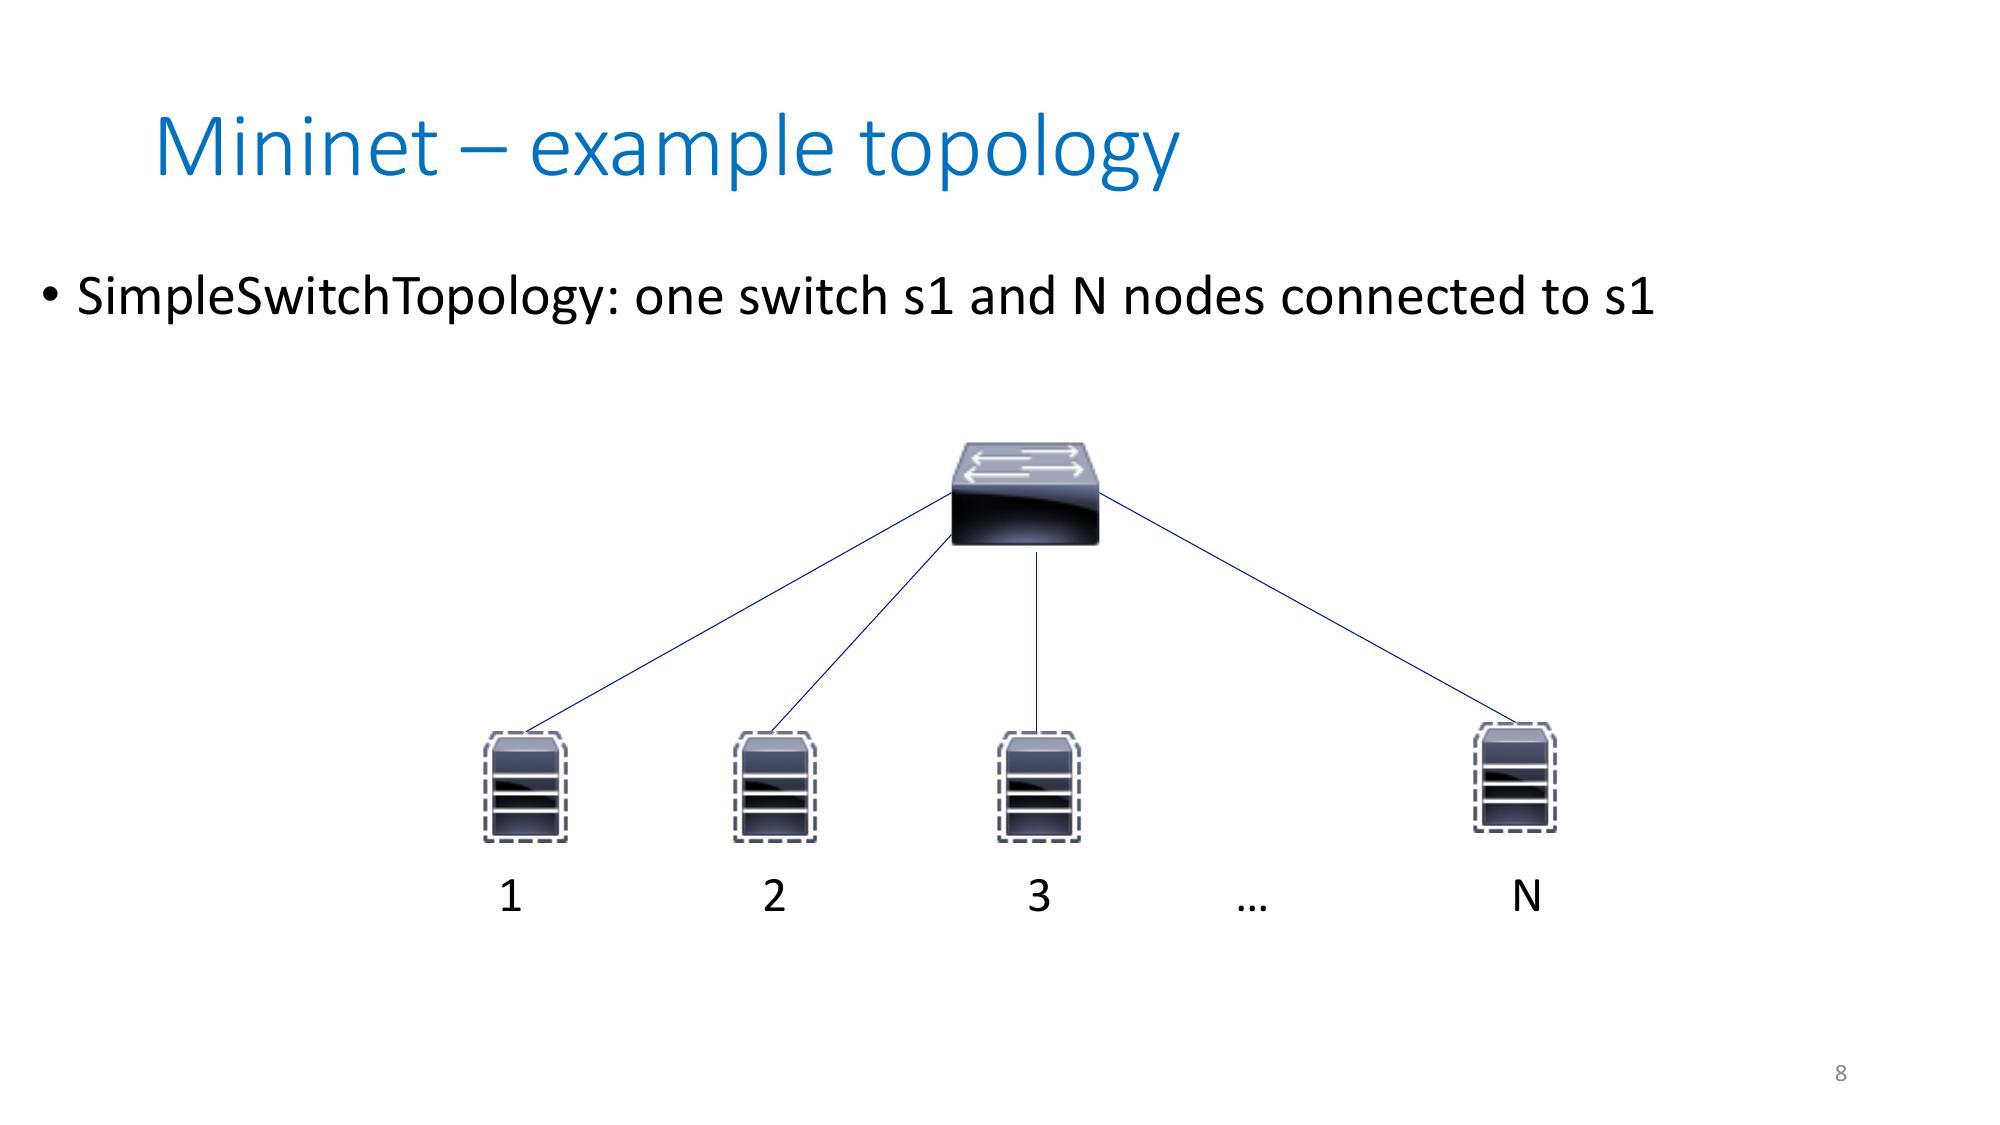
\includegraphics[keepaspectratio]{images/lezione-21-lab-network-emulator-con-comnetsemu-img-01.jpg}}
\caption{Il sito ufficiale di Mininet (http://mininet.org/) con la sua
documentazione, walkthrough e API di riferimento.}
\end{figure}

\subsubsection{Come funziona internamente
Mininet}\label{come-funziona-internamente-mininet}

Gli host di Mininet sono \textbf{processi} che condividono lo stesso
kernel OS, gli stessi PID e file system. Ogni host ha però uno stack di
rete \textbf{indipendente}, realizzato tramite i \emph{network
namespace} di Linux.

\begin{calloutdefinition}{Network Namespace}

Un \emph{network namespace} fornisce uno stack di rete isolato. I
processi al suo interno hanno il proprio set di risorse di rete:
interfacce virtuali, tabelle ARP, tabelle di routing. Un nodo virtuale
di rete è semplicemente una shell in un network namespace.

\end{calloutdefinition}

\subsubsection{Topologie in Mininet}\label{topologie-in-mininet}

Una topologia Mininet è composta da entità come \texttt{Host},
\texttt{Switch}, \texttt{Controller} e \texttt{Link}. È possibile creare
topologie custom tramite script Python estendendo la classe
\texttt{mininet.topo.Topo} e sovrascrivendo il metodo \texttt{build()}.

Il comando più semplice per avviare Mininet con una topologia di default
è:

\begin{Shaded}
\begin{Highlighting}[]
\FunctionTok{sudo}\NormalTok{ mn}
\end{Highlighting}
\end{Shaded}

Questo inizializza una topologia predefinita e lancia la CLI
interattiva.

\paragraph{Esempio:
SimpleSwitchTopology}\label{esempio-simpleswitchtopology}

\begin{figure}
\centering
\pandocbounded{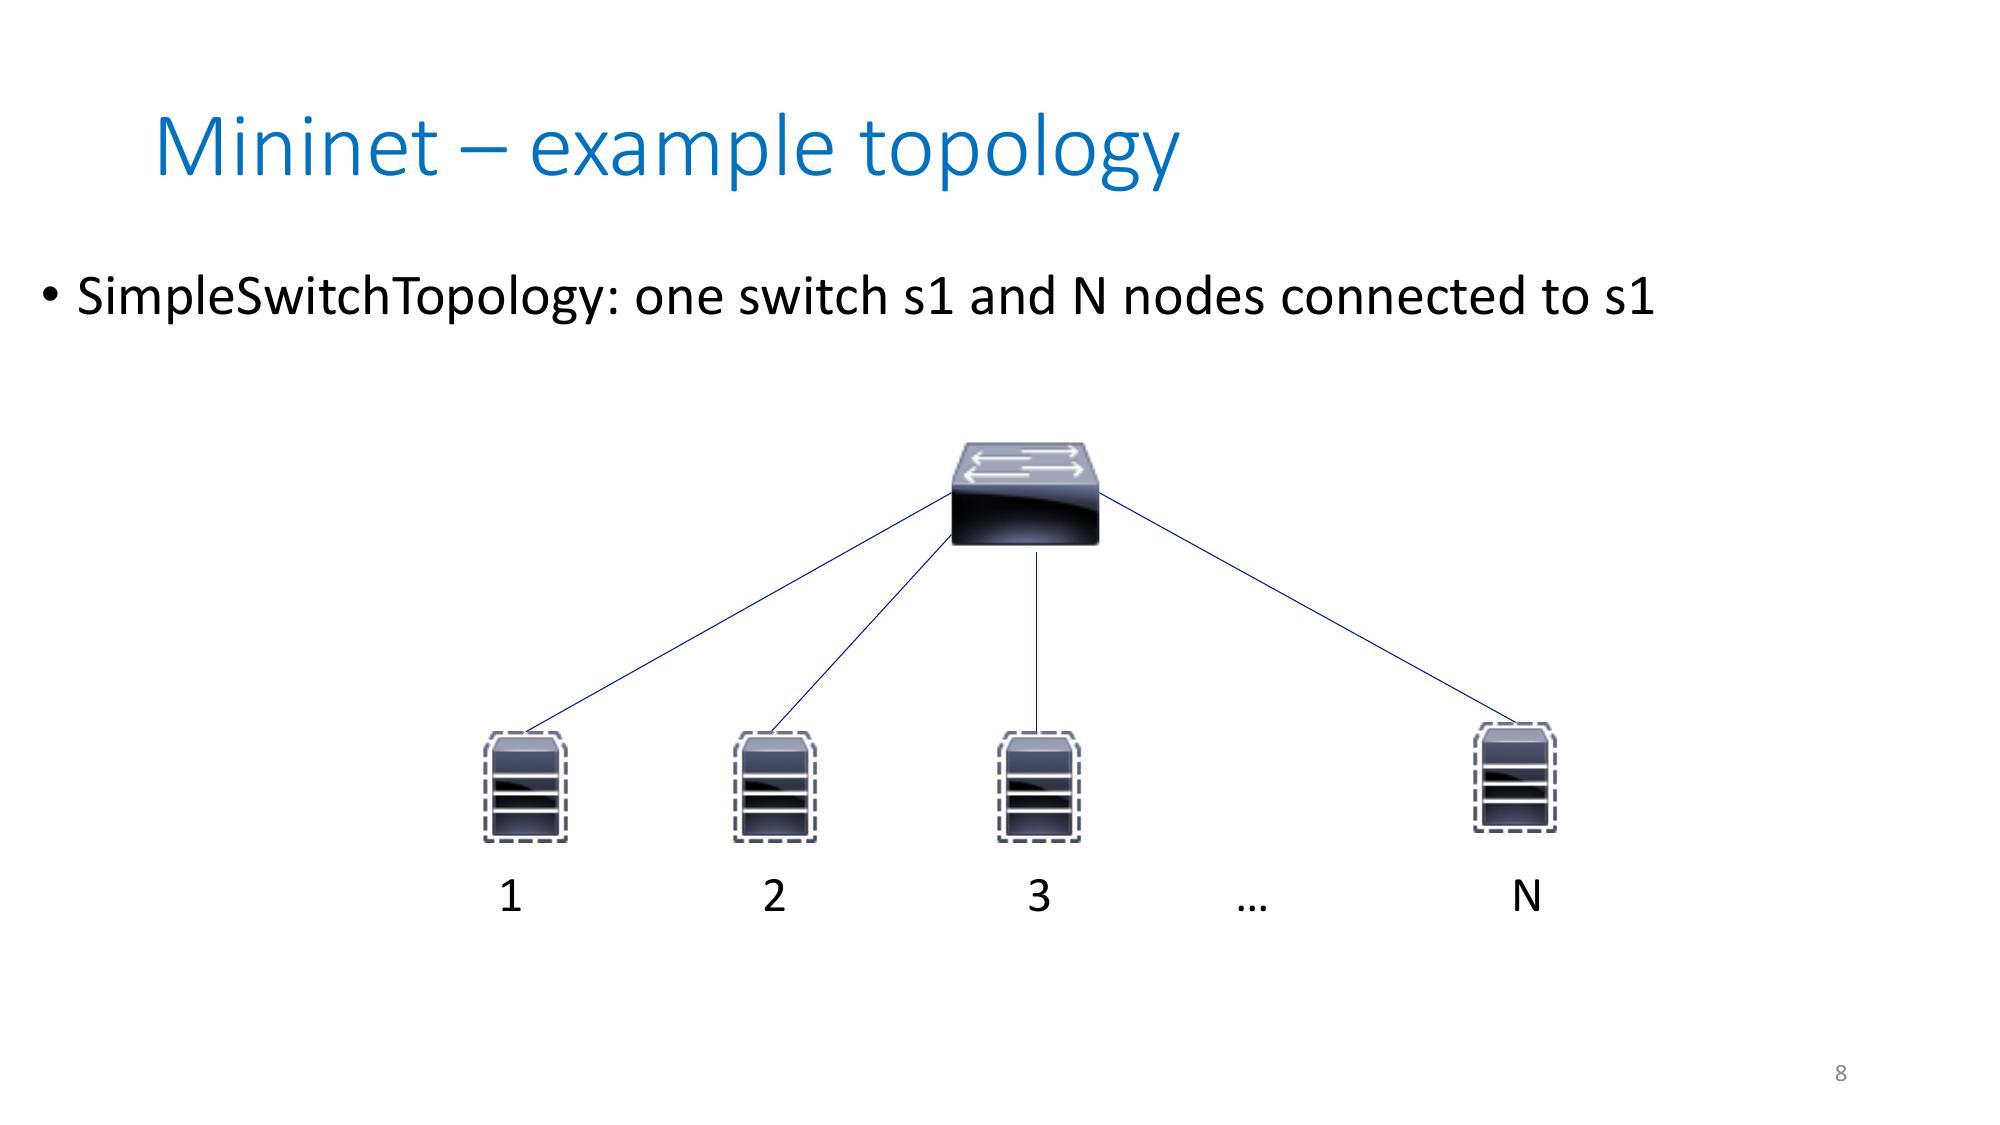
\includegraphics[keepaspectratio]{images/lezione-21-lab-network-emulator-con-comnetsemu-img-02.jpg}}
\caption{SimpleSwitchTopology: uno switch centrale connesso a N host
tramite link individuali.}
\end{figure}

\begin{callouttip}{Principali classi e metodi Mininet}

\begin{itemize}
\tightlist
\item
  \texttt{Topo.addSwitch()} --- aggiunge uno switch alla topologia
\item
  \texttt{Topo.addHost()} --- aggiunge un host alla topologia
\item
  \texttt{Topo.addLink()} --- aggiunge un link bidirezionale
\item
  \texttt{Mininet.start()} / \texttt{Mininet.stop()} --- avvia/ferma la
  rete
\item
  \texttt{Mininet.pingAll()} --- testa la connettività fra tutti i nodi
\item
  Documentazione API: http://mininet.org/api/annotated.html
\end{itemize}

\end{callouttip}

\subsubsection{CLI di Mininet}\label{cli-di-mininet}

La \textbf{CLI} di Mininet è uno strumento interattivo molto utile
durante gli esperimenti. Si invoca passando l'oggetto rete al
costruttore \texttt{CLI(net)}. I comandi principali sono:

\begin{verbatim}
mininet> net             # mostra la topologia
mininet> pingall         # testa la connettività tra tutti i nodi
mininet> h1 ping h2      # ping da h1 verso h2
mininet> h1 ip a         # mostra le interfacce di h1
mininet> iperf h1 h2     # misura il throughput tra h1 e h2
mininet> links           # mostra tutti i link attivi
mininet> h1 ip link show type veth   # mostra le interfacce veth di h1
mininet> sh ovs-vsctl show           # mostra la configurazione del virtual switch
\end{verbatim}

\subsubsection{Veth pairs e piano dati}\label{veth-pairs-e-piano-dati}

Ogni host Mininet può avere un'interfaccia Ethernet virtuale chiamata
\textbf{veth} (\emph{Virtual Ethernet Device}). I dispositivi veth
vengono sempre creati in coppie interconnesse: i pacchetti trasmessi su
un'interfaccia sono immediatamente ricevuti dall'altra. Si può pensare a
un veth come a un cavo Ethernet reale che collega due dispositivi.

\begin{figure}
\centering
\pandocbounded{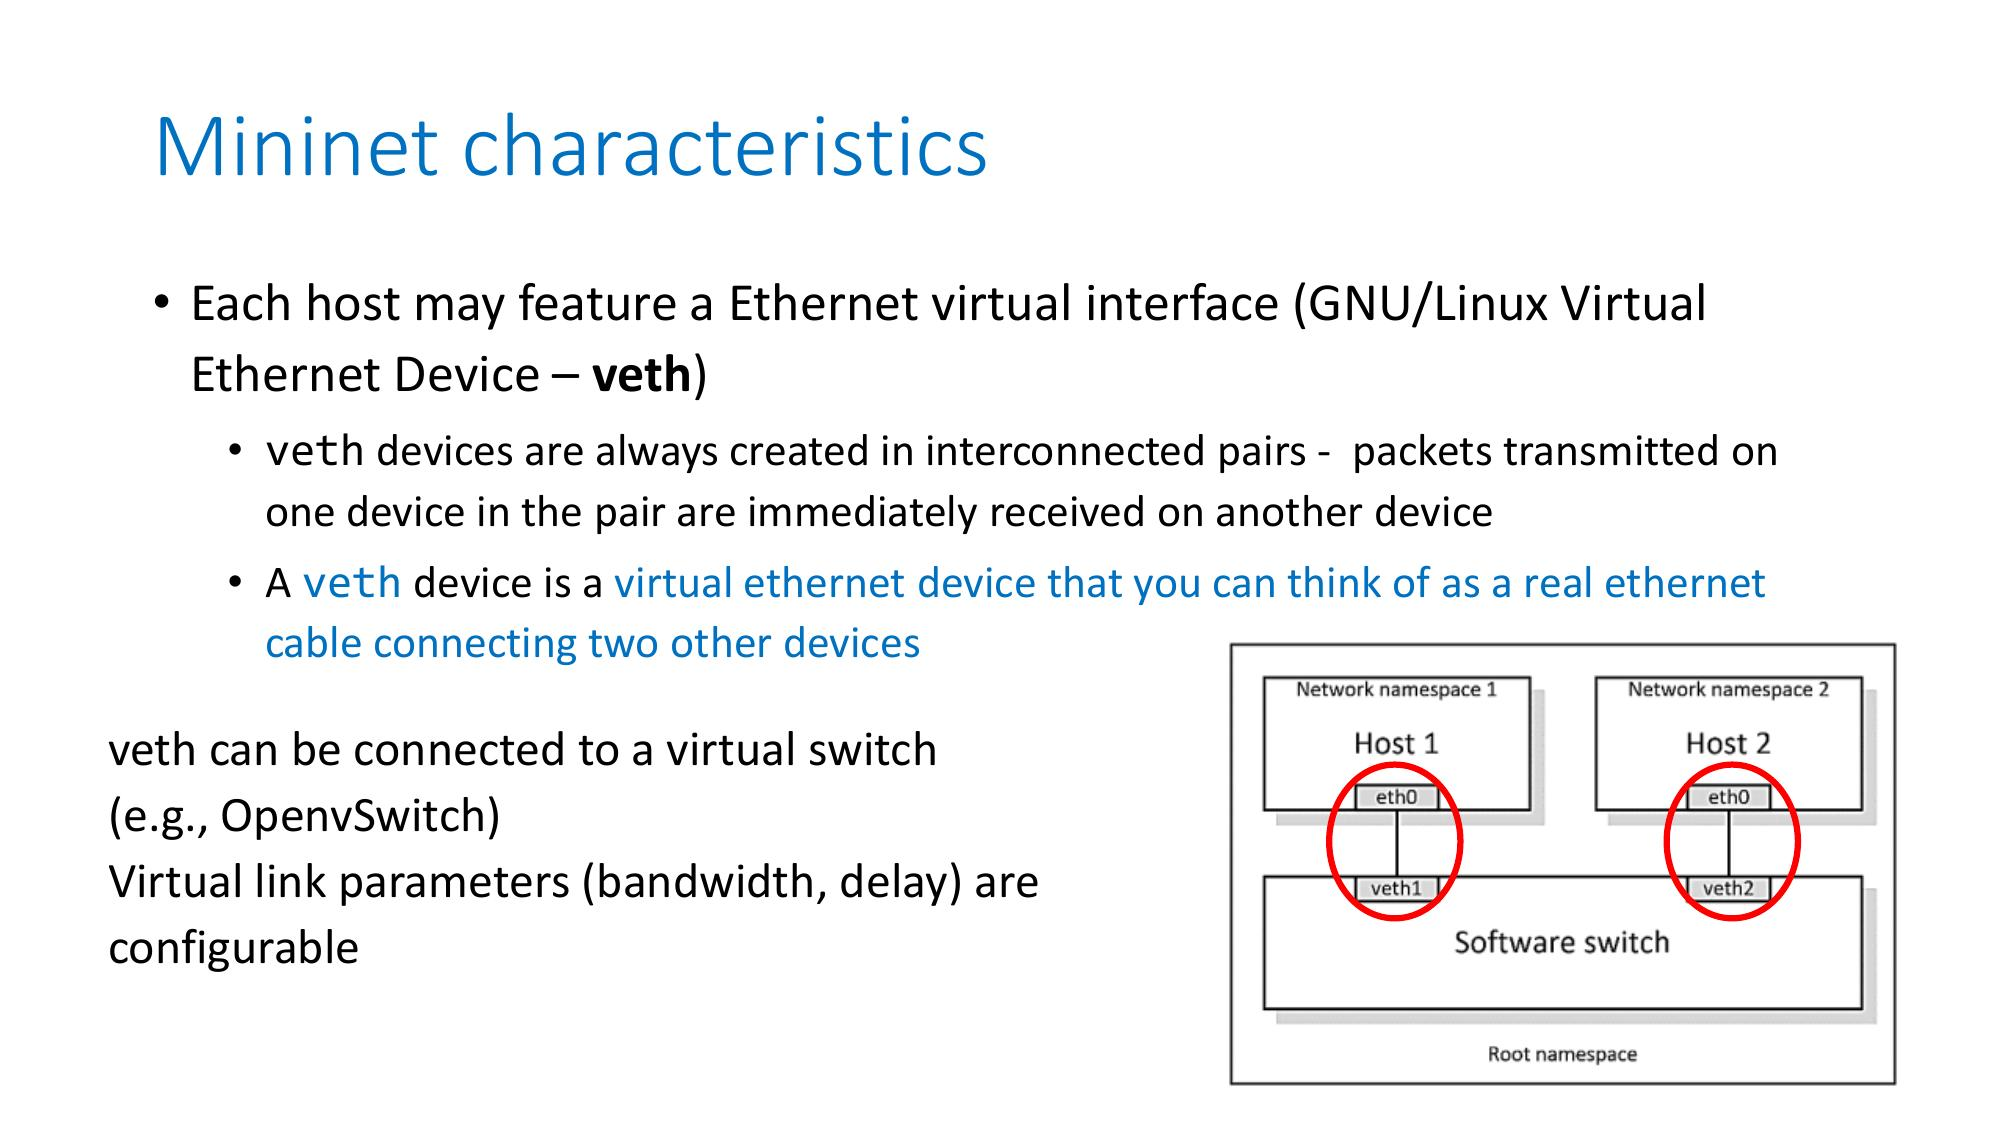
\includegraphics[keepaspectratio]{images/lezione-21-lab-network-emulator-con-comnetsemu-img-03.jpg}}
\caption{Architettura delle veth pairs: Host 1 e Host 2 hanno ciascuno
il proprio network namespace con interfacce veth collegate tramite un
software switch nel Root Namespace.}
\end{figure}

Le coppie veth possono essere connesse a un virtual switch (ad esempio
\textbf{OpenvSwitch}). I parametri del link virtuale come bandwidth e
delay sono configurabili.

\begin{figure}
\centering
\pandocbounded{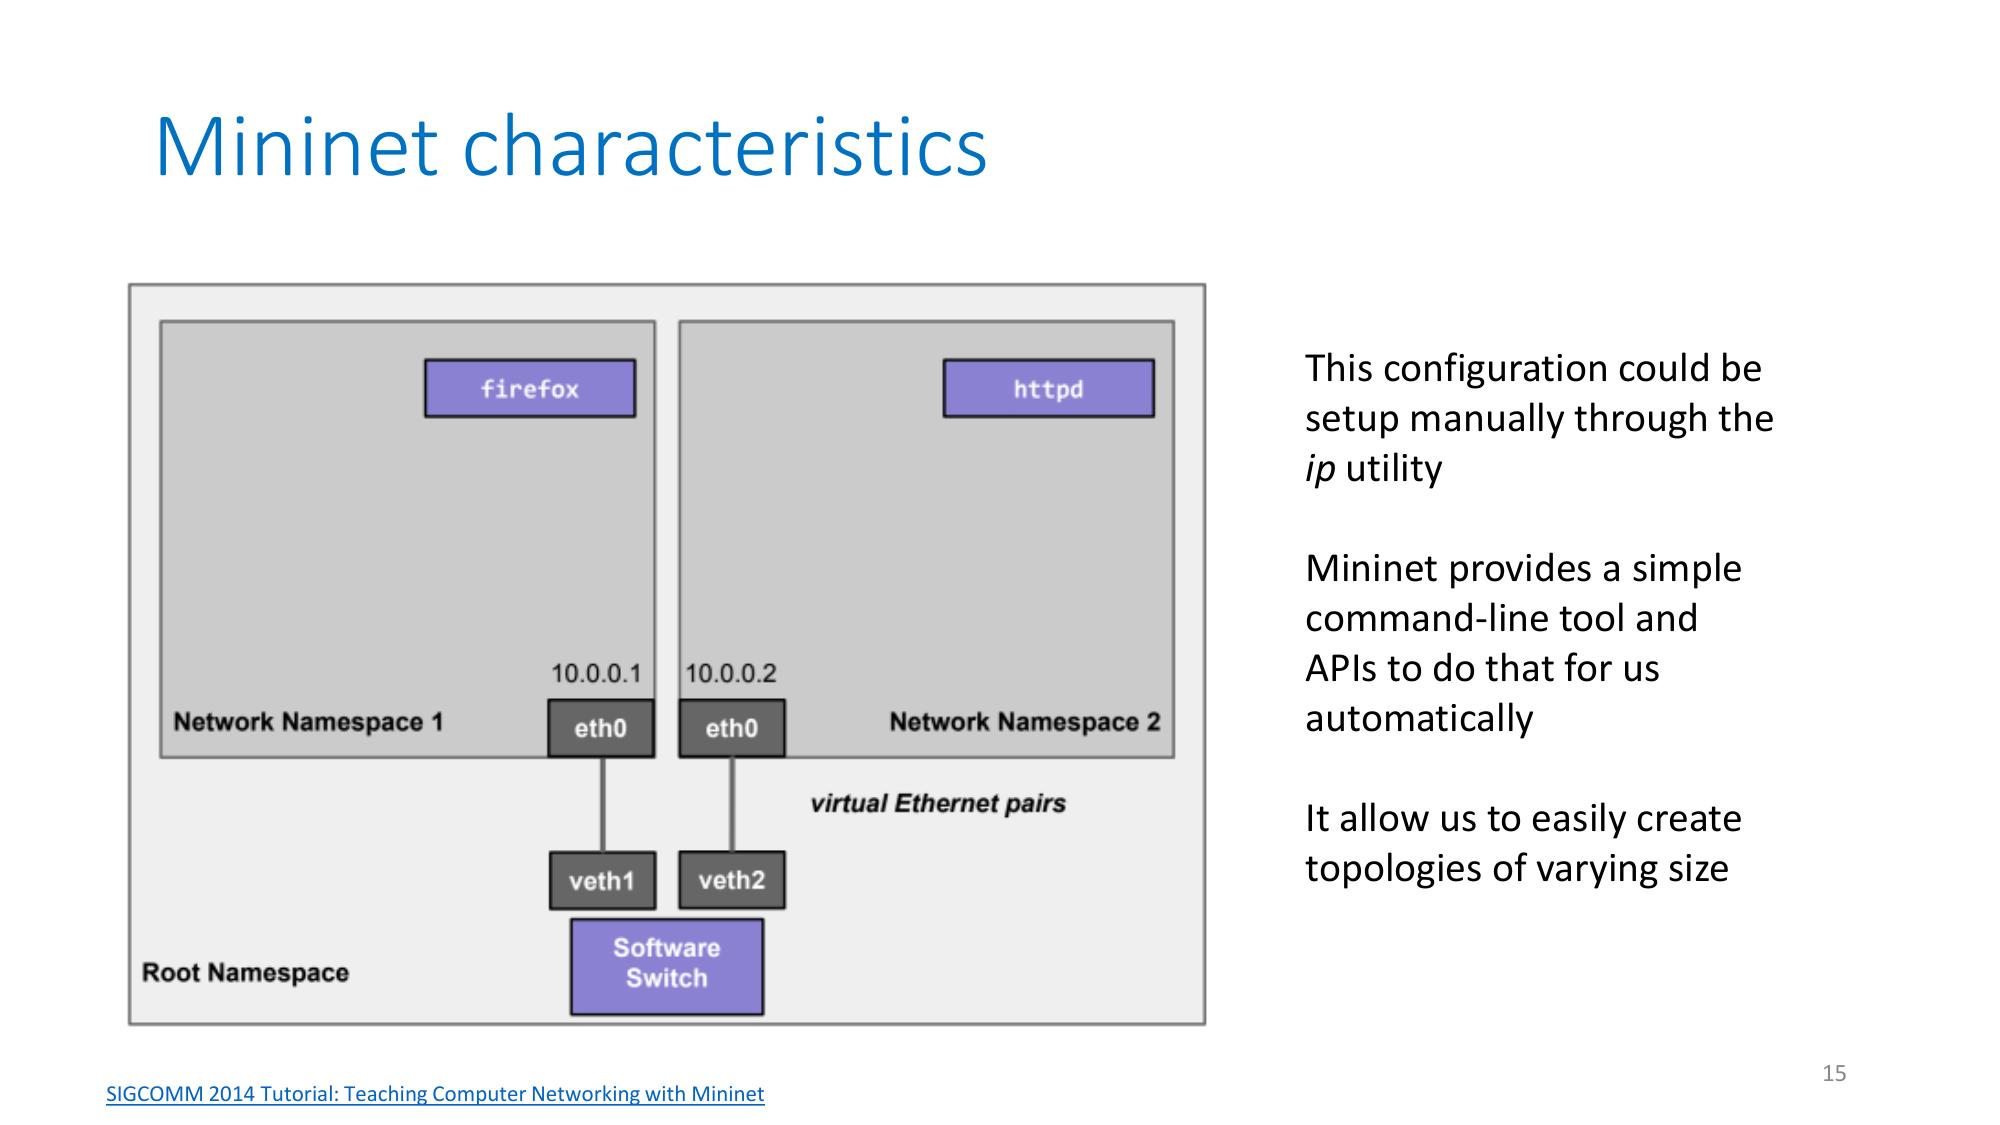
\includegraphics[keepaspectratio]{images/lezione-21-lab-network-emulator-con-comnetsemu-img-04.jpg}}
\caption{Il piano dati di Mininet: due namespace separati collegati
tramite virtual Ethernet pairs e un Software Switch nel Root Namespace.
Mininet gestisce automaticamente questa configurazione al posto
dell'utility \protect\texttt{ip}.}
\end{figure}

\paragraph{Linux Traffic Control (tc)}\label{linux-traffic-control-tc}

Mininet usa \texttt{tc} (\emph{traffic control}) per configurare le
caratteristiche dei link virtuali:

\begin{Shaded}
\begin{Highlighting}[]
\CommentTok{\#\# Aggiunge 100ms di delay + jitter di ±10ms sull\textquotesingle{}interfaccia eth0}
\ExtensionTok{tc}\NormalTok{ qdisc add dev eth0 root netem delay 100ms 10ms}

\CommentTok{\#\# Da dentro Mininet, su h1:}
\ExtensionTok{h1}\NormalTok{ tc qdisc add dev h1{-}eth0 root netem delay 100ms 10ms}
\ExtensionTok{h1}\NormalTok{ tc qdisc show dev h1{-}eth0}
\ExtensionTok{h1}\NormalTok{ tc qdisc del dev h1{-}eth0 root}
\end{Highlighting}
\end{Shaded}

\begin{center}\rule{0.5\linewidth}{0.5pt}\end{center}

\subsection{Architettura di
ComNetsEmu}\label{architettura-di-comnetsemu}

ComNetsEmu estende Mininet sostituendo il tipo di host di default con
\textbf{container Docker}. Questo approccio si chiama
\emph{Docker-in-Docker} (o \emph{sibling containers}): si ha un
\texttt{DockerHost} con container Docker interni che emulano host fisici
che eseguono applicazioni containerizzate.

\begin{figure}
\centering
\pandocbounded{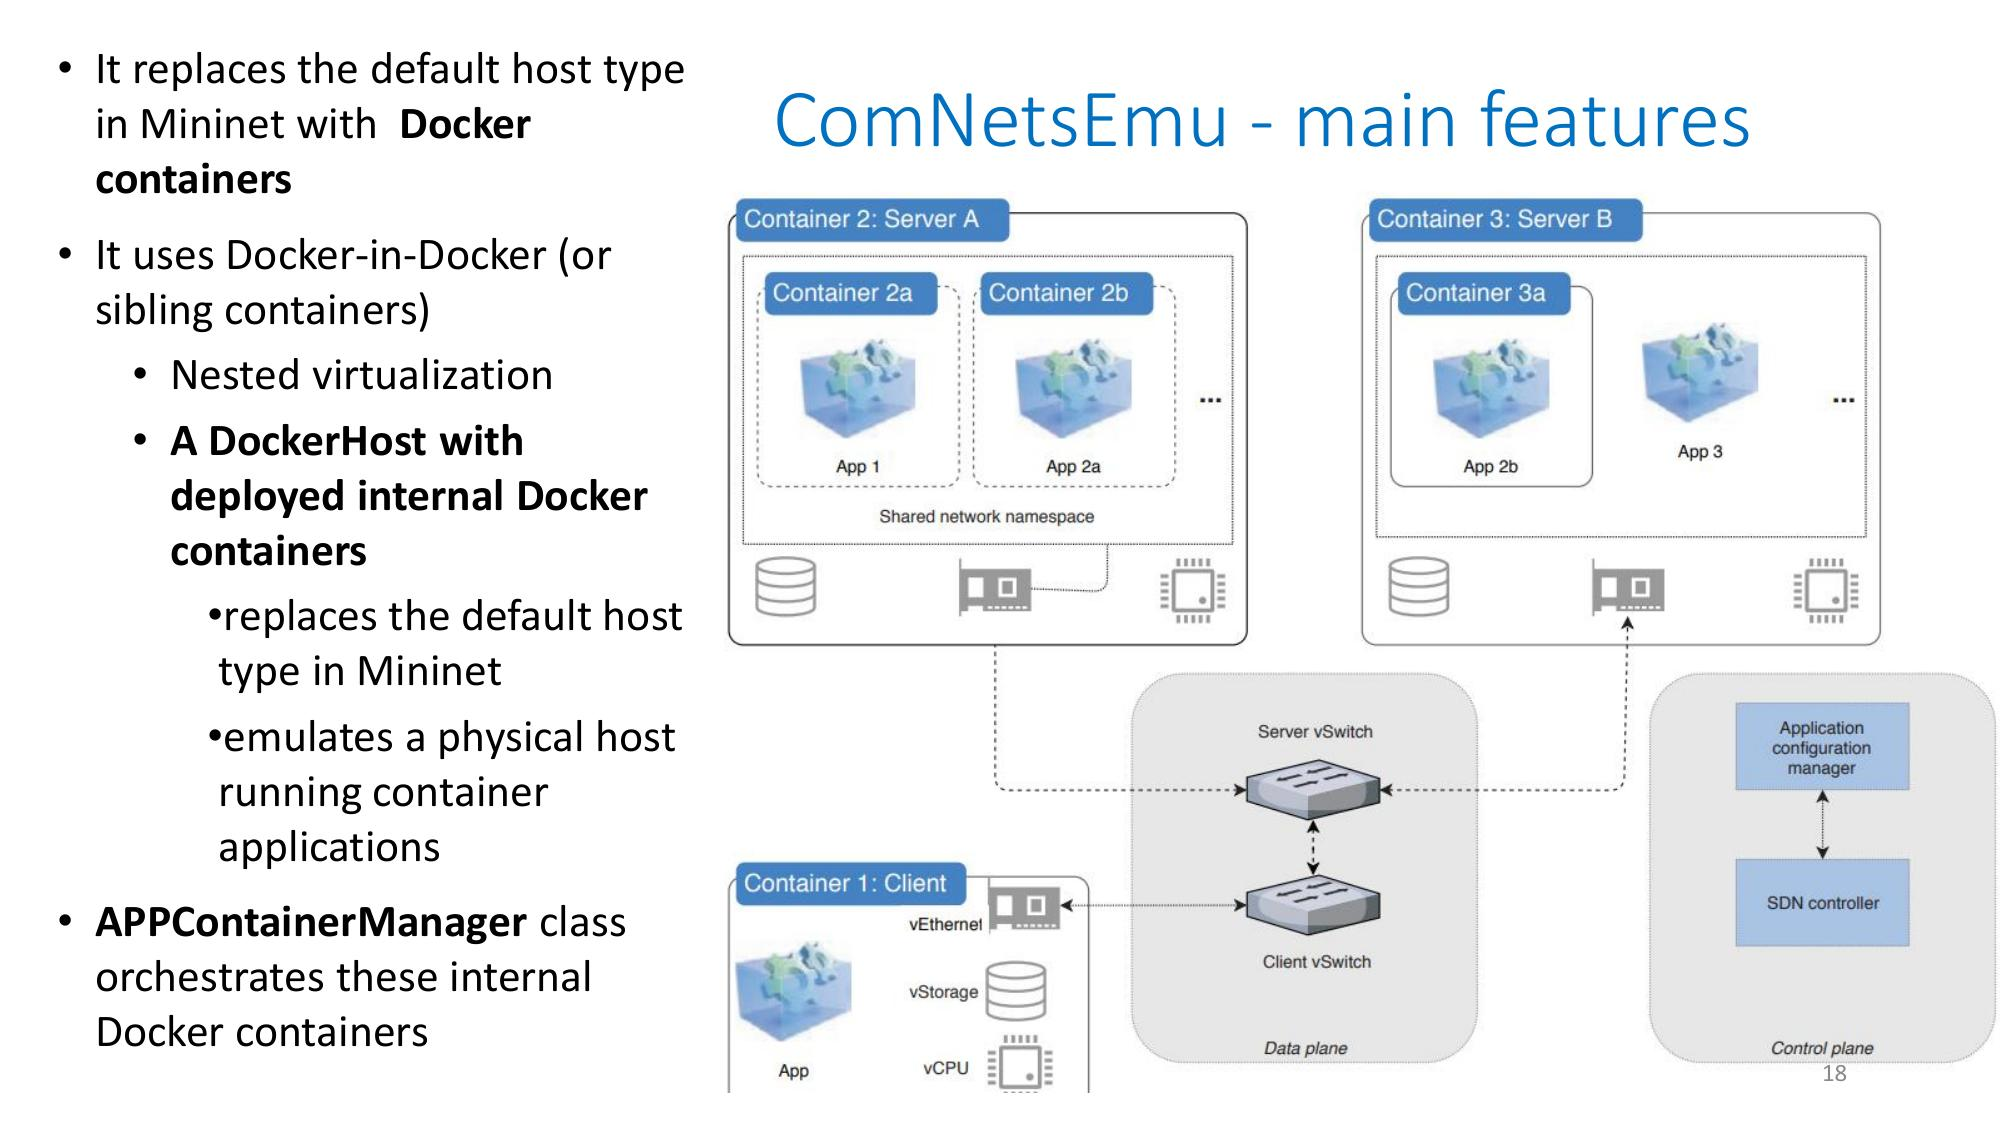
\includegraphics[keepaspectratio]{images/lezione-21-lab-network-emulator-con-comnetsemu-img-05.jpg}}
\caption{Architettura ComNetsEmu: i container rappresentano applicazioni
su host virtuali; il piano dati è gestito da virtual switch; il control
plane è affidato a un SDN controller.}
\end{figure}

La classe \texttt{APPContainerManager} orchestra i container Docker
interni. Ogni \texttt{DockerHost} rimpiazza il tipo host di Mininet ed
emula un host fisico che gira applicazioni containerizzate.

\subsubsection{Struttura del repository}\label{struttura-del-repository}

{\def\LTcaptype{none} % do not increment counter
\begin{longtable}[]{@{}ll@{}}
\toprule\noalign{}
Cartella/File & Contenuto \\
\midrule\noalign{}
\endhead
\bottomrule\noalign{}
\endlastfoot
\texttt{comnetsemu/} & Modulo Python che estende Mininet \\
\texttt{examples/} & Esempi per iniziare con le API ComNetsEmu \\
\texttt{app/} & Esempi di network slicing, SDN, ecc. \\
\texttt{util/} & Script per la gestione dell'ambiente \\
\texttt{test\_containers/} & Dockerfile per i programmi di esempio \\
\texttt{Vagrantfile} & File Vagrant per il setup della VM \\
\end{longtable}
}

\begin{center}\rule{0.5\linewidth}{0.5pt}\end{center}

\subsection{Setup dell'ambiente}\label{setup-dellambiente}

\begin{calloutwarning}{Prerequisiti da installare prima del laboratorio}

L'installazione richiede circa \textbf{15 minuti} la prima volta.
Completala prima della lezione di laboratorio.

\end{calloutwarning}

\subsubsection{Dipendenze}\label{dipendenze}

ComNetsEmu viene eseguito in una VM gestita da \textbf{Vagrant}. Le
dipendenze da installare sul proprio sistema host sono:

\begin{itemize}
\tightlist
\item
  \textbf{Vagrant} \textgreater= v2.2.5 ---
  https://developer.hashicorp.com/vagrant/downloads
\item
  \textbf{VirtualBox} \textgreater= v6.0 ---
  https://www.virtualbox.org/wiki/Downloads
\end{itemize}

Una volta avviata la VM, al suo interno saranno già presenti: - Mininet
+ OpenVswitch + Wireshark - Ryu SDN controller - Docker Engine

\subsubsection{Installazione su Linux e
Windows}\label{installazione-su-linux-e-windows}

Segui le istruzioni ufficiali:
https://stevelorenz.github.io/comnetsemu/installation.html\#option-1-install-in-a-vagrant-managed-vm-highly-recommended

\begin{Shaded}
\begin{Highlighting}[]
\BuiltInTok{cd}\NormalTok{ \textasciitilde{}}
\FunctionTok{git}\NormalTok{ clone https://git.comnets.net/public{-}repo/comnetsemu.git}
\BuiltInTok{cd}\NormalTok{ ./comnetsemu}
\end{Highlighting}
\end{Shaded}

Prima di avviare la VM, è necessario modificare un Dockerfile.

\subsubsection{Modifica obbligatoria:
Dockerfile.dev\_test}\label{modifica-obbligatoria-dockerfile.dev_test}

\begin{calloutwarning}{Passo critico — da non saltare}

Prima di eseguire \texttt{vagrant\ up}, devi modificare il file
\texttt{Dockerfile.dev\_test} aggiungendo \texttt{netcat} alle
dipendenze. Senza questa modifica il client TCP dell'esempio non
funzionerà.

\end{calloutwarning}

\begin{Shaded}
\begin{Highlighting}[]
\BuiltInTok{cd}\NormalTok{ test\_containers}
\CommentTok{\#\# Apri il file Dockerfile.dev\_test e aggiungi la riga "netcat \textbackslash{}\textbackslash{}" come mostrato nell\textquotesingle{}immagine}
\end{Highlighting}
\end{Shaded}

\begin{figure}
\centering
\pandocbounded{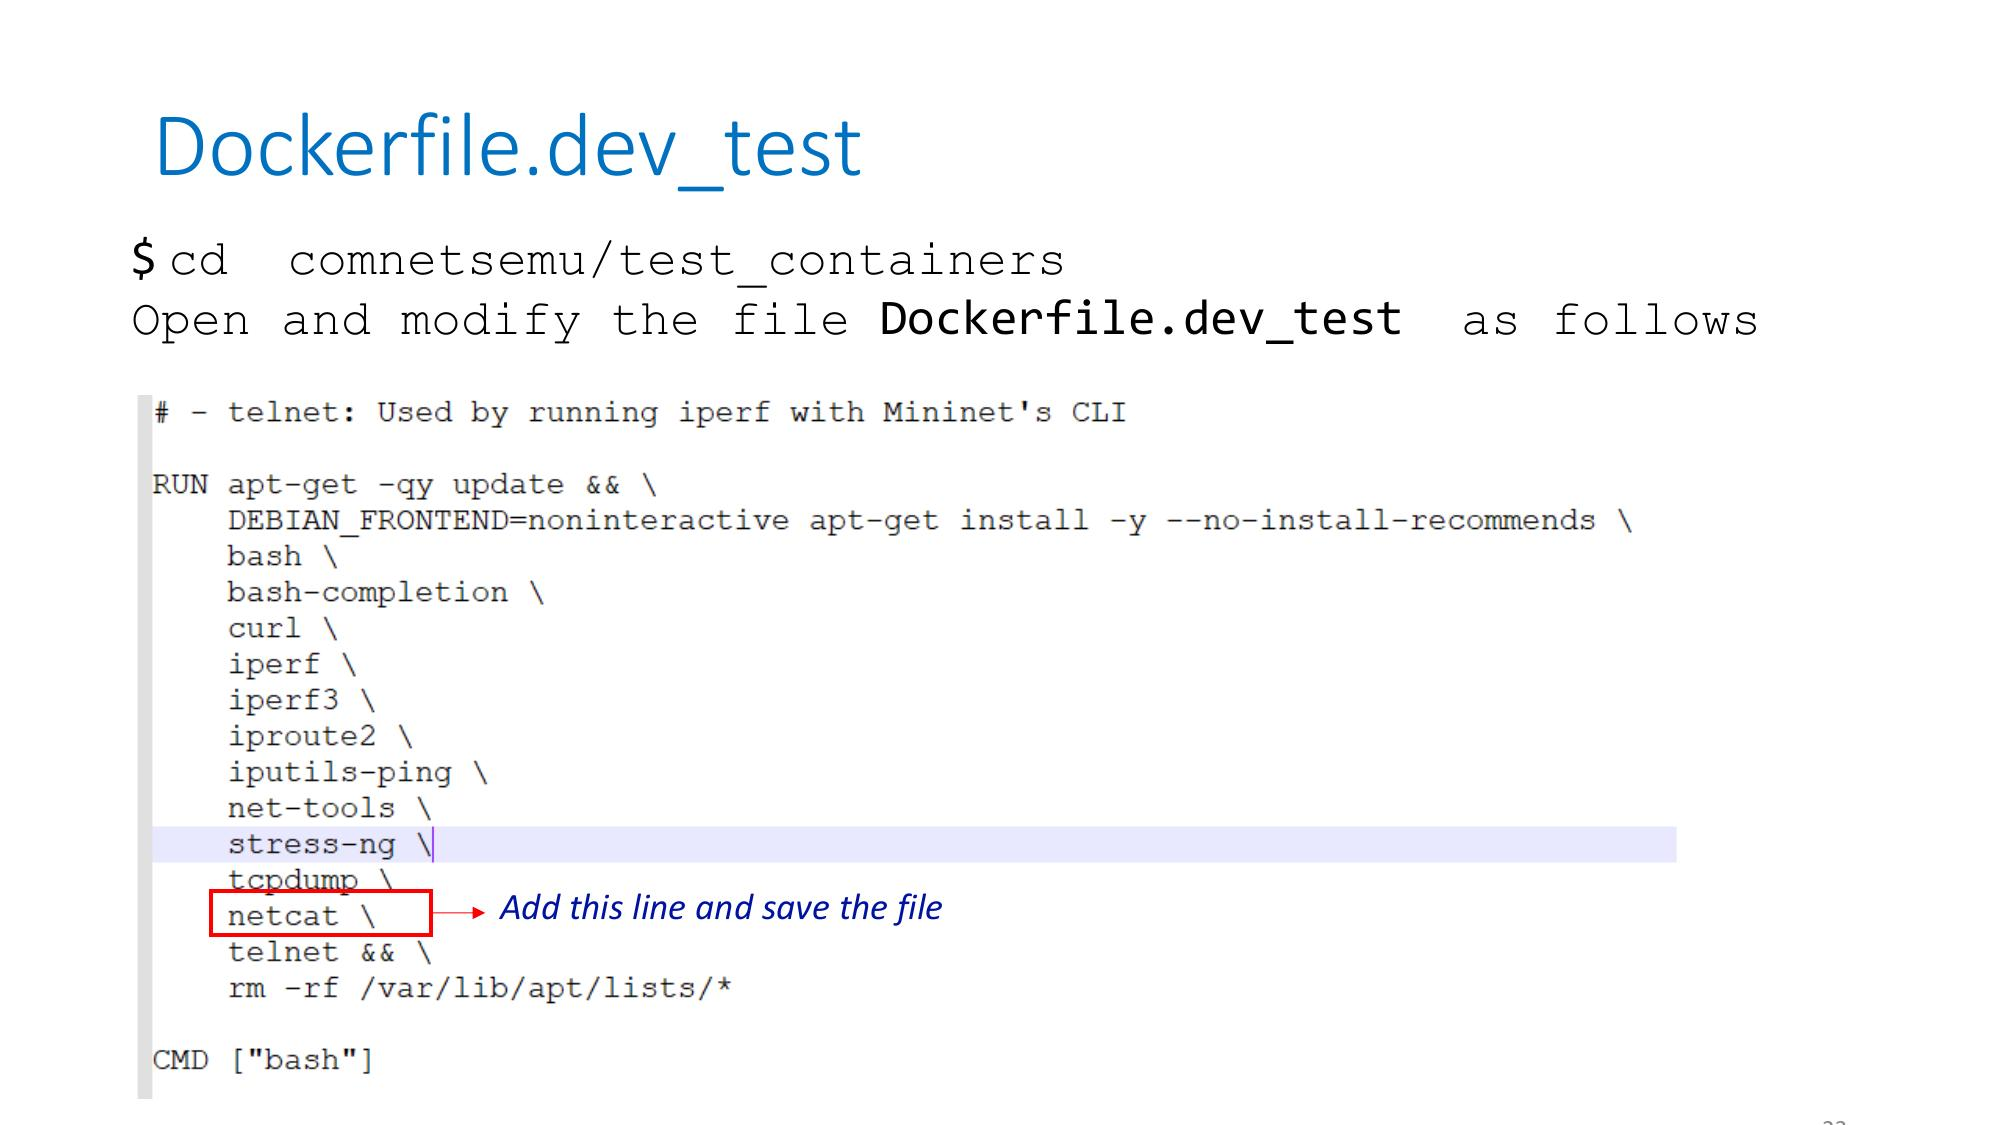
\includegraphics[keepaspectratio]{images/lezione-21-lab-network-emulator-con-comnetsemu-img-06.jpg}}
\caption{Il file \protect\texttt{Dockerfile.dev\_test}: aggiungere la
riga \protect\texttt{netcat\ \textbackslash{}\textbackslash{}} prima di
\protect\texttt{telnet\ \textbackslash{}\textbackslash{}} nella lista
dei pacchetti da installare con \protect\texttt{apt-get}.}
\end{figure}

Il file modificato deve includere \texttt{netcat\ \textbackslash{}}
nella lista dei pacchetti \texttt{apt-get\ install}. Dopo la modifica,
salva il file e torna nella directory principale.

\subsubsection{Avvio della VM}\label{avvio-della-vm}

\begin{Shaded}
\begin{Highlighting}[]
\BuiltInTok{cd}\NormalTok{ ..}
\ExtensionTok{vagrant}\NormalTok{ up comnetsemu}
\CommentTok{\#\# Attendi circa 15 minuti la prima volta}
\end{Highlighting}
\end{Shaded}

Quando la VM è pronta, il banner di ComNetsEmu viene stampato a schermo.
A quel punto:

\begin{Shaded}
\begin{Highlighting}[]
\CommentTok{\#\# Accedi alla VM via SSH}
\ExtensionTok{vagrant}\NormalTok{ ssh comnetsemu}

\CommentTok{\#\# Quando hai finito, ferma la VM sul terminale locale}
\ExtensionTok{vagrant}\NormalTok{ halt}
\end{Highlighting}
\end{Shaded}

\subsubsection{Installazione su Mac}\label{installazione-su-mac}

\begin{calloutnote}{Mac — Percorso alternativo con Multipass}

L'installazione con Vagrant potrebbe non funzionare su host Mac. In quel
caso usa \textbf{Multipass}, un gestore di VM leggero sviluppato da
Canonical. Segui le istruzioni al punto \textbf{B} di:
https://www.granelli-lab.org/researches/relevant-projects/comnetsemu-labs

\end{calloutnote}

\subsubsection{Installazione su Windows}\label{installazione-su-windows}

Per host Windows, usa \textbf{MobaXterm} come console. Se l'apertura di
xterm nell'emulatore non funziona:

\begin{Shaded}
\begin{Highlighting}[]
\CommentTok{\#\# Salva la configurazione SSH in un file}
\ExtensionTok{vagrant}\NormalTok{ ssh{-}config }\OperatorTok{\textgreater{}}\NormalTok{ vagrant{-}ssh}

\CommentTok{\#\# Connettiti con forwarding X11 abilitato}
\FunctionTok{ssh} \AttributeTok{{-}F}\NormalTok{ vagrant{-}ssh }\AttributeTok{{-}Y}\NormalTok{ comnetsemu}

\CommentTok{\#\# Testa il forwarding X11}
\ExtensionTok{xeyes}
\CommentTok{\#\# oppure}
\ExtensionTok{xterm}
\end{Highlighting}
\end{Shaded}

\begin{center}\rule{0.5\linewidth}{0.5pt}\end{center}

\subsection{Primo esempio: Echo Server}\label{primo-esempio-echo-server}

L'esempio \texttt{echo\_server} mostra l'uso base dell'emulatore: due
host emulati connessi tra loro tramite due switch, dove uno fa da client
e l'altro ospita un server TCP che rimanda indietro ciò che riceve.

\begin{figure}
\centering
\pandocbounded{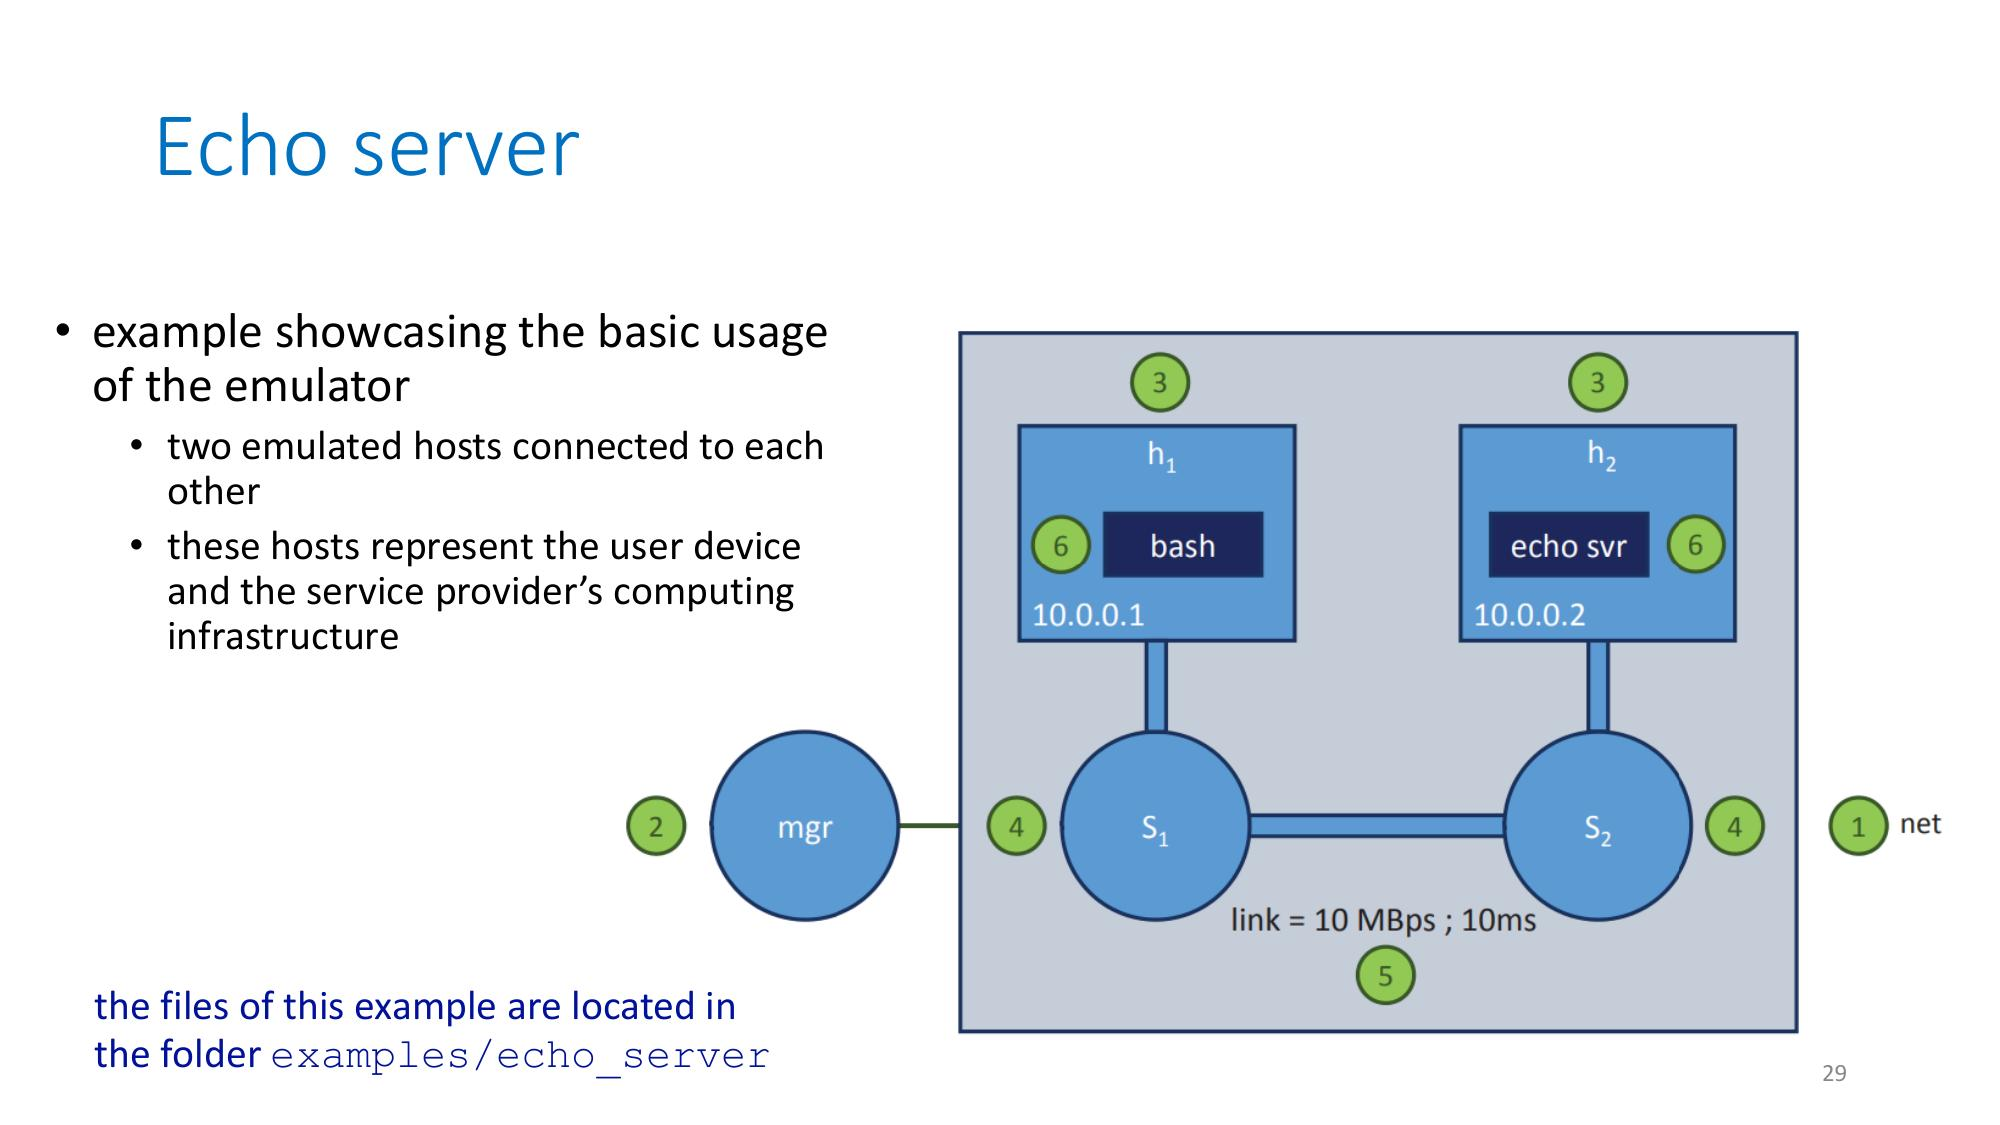
\includegraphics[keepaspectratio]{images/lezione-21-lab-network-emulator-con-comnetsemu-img-07.jpg}}
\caption{Topologia dell'echo server: \protect\texttt{h1} (10.0.0.1) con
container \protect\texttt{bash} e \protect\texttt{h2} (10.0.0.2) con
container \protect\texttt{echo\_server}, collegati da due switch con
link da 10 Mbps e 10ms di delay.}
\end{figure}

\subsubsection{Struttura del progetto}\label{struttura-del-progetto}

\begin{Shaded}
\begin{Highlighting}[]
\BuiltInTok{cd}\NormalTok{ \textasciitilde{}/comnetsemu/examples}
\FunctionTok{mkdir}\NormalTok{ echoMCPS}
\BuiltInTok{cd}\NormalTok{ echoMCPS}
\end{Highlighting}
\end{Shaded}

Il progetto richiede quattro file:

{\def\LTcaptype{none} % do not increment counter
\begin{longtable}[]{@{}ll@{}}
\toprule\noalign{}
File & Scopo \\
\midrule\noalign{}
\endhead
\bottomrule\noalign{}
\endlastfoot
\texttt{server.py} & Applicazione server TCP (echo) \\
\texttt{Dockerfile} & Containerizza l'applicazione server \\
\texttt{build\_docker\_image.sh} & Script per costruire l'immagine
Docker \\
\texttt{topology.py} & Definisce la topologia ComNetsEmu \\
\end{longtable}
}

\subsubsection{File 1: server.py}\label{file-1-server.py}

Il server apre un socket TCP sulla porta 65000, accetta connessioni e
rimanda indietro ogni segmento ricevuto (echo):

\begin{Shaded}
\begin{Highlighting}[]
\ImportTok{import}\NormalTok{ socket}

\CommentTok{\#\# Crea un socket TCP/IP}
\NormalTok{sock }\OperatorTok{=}\NormalTok{ socket.socket(socket.AF\_INET, socket.SOCK\_STREAM)}

\CommentTok{\#\# Bind sulla porta 65000 (su tutte le interfacce)}
\NormalTok{server\_address }\OperatorTok{=}\NormalTok{ (}\StringTok{""}\NormalTok{, }\DecValTok{65000}\NormalTok{)}
\BuiltInTok{print}\NormalTok{(}\StringTok{"starting up on }\SpecialCharTok{\{\}}\StringTok{ port }\SpecialCharTok{\{\}}\StringTok{"}\NormalTok{.}\BuiltInTok{format}\NormalTok{(}\OperatorTok{*}\NormalTok{server\_address))}
\NormalTok{sock.bind(server\_address)}

\CommentTok{\#\# In ascolto per connessioni in ingresso}
\NormalTok{sock.listen(}\DecValTok{1}\NormalTok{)}

\ControlFlowTok{while} \VariableTok{True}\NormalTok{:}
    \BuiltInTok{print}\NormalTok{(}\StringTok{"waiting for a connection"}\NormalTok{)}
\NormalTok{    connection, client\_address }\OperatorTok{=}\NormalTok{ sock.accept()}
    \ControlFlowTok{try}\NormalTok{:}
        \BuiltInTok{print}\NormalTok{(}\StringTok{"connection from"}\NormalTok{, client\_address)}
        \ControlFlowTok{while} \VariableTok{True}\NormalTok{:}
\NormalTok{            data }\OperatorTok{=}\NormalTok{ connection.recv(}\DecValTok{16}\NormalTok{)}
            \BuiltInTok{print}\NormalTok{(}\StringTok{"received }\SpecialCharTok{\{!r\}}\StringTok{"}\NormalTok{.}\BuiltInTok{format}\NormalTok{(data))}
            \ControlFlowTok{if}\NormalTok{ data:}
                \BuiltInTok{print}\NormalTok{(}\StringTok{"sending data back to the client"}\NormalTok{)}
\NormalTok{                connection.sendall(data)}
            \ControlFlowTok{else}\NormalTok{:}
                \BuiltInTok{print}\NormalTok{(}\StringTok{"no data from"}\NormalTok{, client\_address)}
                \ControlFlowTok{break}
    \ControlFlowTok{finally}\NormalTok{:}
\NormalTok{        connection.close()}
\end{Highlighting}
\end{Shaded}

\subsubsection{File 2: Dockerfile}\label{file-2-dockerfile}

\begin{Shaded}
\begin{Highlighting}[]
\KeywordTok{FROM}\NormalTok{ python:3.6{-}alpine3.9}
\KeywordTok{COPY}\NormalTok{ ./server.py /home/server.py}
\KeywordTok{CMD} \ExtensionTok{python}\NormalTok{ /home/server.py}
\end{Highlighting}
\end{Shaded}

\subsubsection{File 3:
build\_docker\_image.sh}\label{file-3-build_docker_image.sh}

\begin{Shaded}
\begin{Highlighting}[]
\ExtensionTok{docker}\NormalTok{ build }\AttributeTok{{-}t}\NormalTok{ echo\_server }\AttributeTok{{-}{-}file}\NormalTok{ ./Dockerfile .}
\end{Highlighting}
\end{Shaded}

Per costruire l'immagine:

\begin{Shaded}
\begin{Highlighting}[]
\FunctionTok{bash}\NormalTok{ build\_docker\_image.sh}
\end{Highlighting}
\end{Shaded}

\subsubsection{File 4: topology.py}\label{file-4-topology.py}

\begin{Shaded}
\begin{Highlighting}[]
\ImportTok{from}\NormalTok{ comnetsemu.net }\ImportTok{import}\NormalTok{ Containernet, VNFManager}
\ImportTok{from}\NormalTok{ comnetsemu.cli }\ImportTok{import}\NormalTok{ spawnXtermDocker}
\ImportTok{from}\NormalTok{ mininet.node }\ImportTok{import}\NormalTok{ Controller}
\ImportTok{from}\NormalTok{ mininet.link }\ImportTok{import}\NormalTok{ TCLink}
\ImportTok{from}\NormalTok{ mininet.log }\ImportTok{import}\NormalTok{ info}
\ImportTok{from}\NormalTok{ mininet.cli }\ImportTok{import}\NormalTok{ CLI}

\NormalTok{net }\OperatorTok{=}\NormalTok{ Containernet(controller}\OperatorTok{=}\NormalTok{Controller, link}\OperatorTok{=}\NormalTok{TCLink, xterms}\OperatorTok{=}\VariableTok{False}\NormalTok{)}
\NormalTok{mgr }\OperatorTok{=}\NormalTok{ VNFManager(net)}

\ControlFlowTok{try}\NormalTok{:}
\NormalTok{    info(}\StringTok{"*** Add controller}\CharTok{\textbackslash{}n}\StringTok{"}\NormalTok{)}
\NormalTok{    net.addController(}\StringTok{"c0"}\NormalTok{)}

\NormalTok{    info(}\StringTok{"*** Creating hosts}\CharTok{\textbackslash{}n}\StringTok{"}\NormalTok{)}
\NormalTok{    h1 }\OperatorTok{=}\NormalTok{ net.addDockerHost(}\StringTok{"h1"}\NormalTok{, dimage}\OperatorTok{=}\StringTok{"dev\_test"}\NormalTok{,}
\NormalTok{         ip}\OperatorTok{=}\StringTok{"10.0.0.1"}\NormalTok{, docker\_args}\OperatorTok{=}\NormalTok{\{}\StringTok{"hostname"}\NormalTok{: }\StringTok{"h1"}\NormalTok{\})}
\NormalTok{    h2 }\OperatorTok{=}\NormalTok{ net.addDockerHost(}\StringTok{"h2"}\NormalTok{, dimage}\OperatorTok{=}\StringTok{"dev\_test"}\NormalTok{,}
\NormalTok{         ip}\OperatorTok{=}\StringTok{"10.0.0.2"}\NormalTok{, docker\_args}\OperatorTok{=}\NormalTok{\{}\StringTok{"hostname"}\NormalTok{: }\StringTok{"h2"}\NormalTok{\})}

\NormalTok{    info(}\StringTok{"*** Adding switch and links}\CharTok{\textbackslash{}n}\StringTok{"}\NormalTok{)}
\NormalTok{    switch1 }\OperatorTok{=}\NormalTok{ net.addSwitch(}\StringTok{"s1"}\NormalTok{)}
\NormalTok{    switch2 }\OperatorTok{=}\NormalTok{ net.addSwitch(}\StringTok{"s2"}\NormalTok{)}
\NormalTok{    net.addLink(switch1, h1, bw}\OperatorTok{=}\DecValTok{10}\NormalTok{, delay}\OperatorTok{=}\StringTok{"10ms"}\NormalTok{)}
\NormalTok{    net.addLink(switch1, switch2, bw}\OperatorTok{=}\DecValTok{10}\NormalTok{, delay}\OperatorTok{=}\StringTok{"10ms"}\NormalTok{)}
\NormalTok{    net.addLink(switch2, h2, bw}\OperatorTok{=}\DecValTok{10}\NormalTok{, delay}\OperatorTok{=}\StringTok{"10ms"}\NormalTok{)}

\NormalTok{    info(}\StringTok{"}\CharTok{\textbackslash{}n}\StringTok{*** Starting network}\CharTok{\textbackslash{}n}\StringTok{"}\NormalTok{)}
\NormalTok{    net.start()}

    \CommentTok{\# Avvia i container applicativi}
\NormalTok{    srv1 }\OperatorTok{=}\NormalTok{ mgr.addContainer(}\StringTok{"srv1"}\NormalTok{, }\StringTok{"h1"}\NormalTok{, }\StringTok{"dev\_test"}\NormalTok{, }\StringTok{"bash"}\NormalTok{, docker\_args}\OperatorTok{=}\NormalTok{\{\})}
\NormalTok{    srv2 }\OperatorTok{=}\NormalTok{ mgr.addContainer(}\StringTok{"srv2"}\NormalTok{, }\StringTok{"h2"}\NormalTok{, }\StringTok{"echo\_server"}\NormalTok{,}
           \StringTok{"python /home/server.py"}\NormalTok{, docker\_args}\OperatorTok{=}\NormalTok{\{\})}

    \CommentTok{\# spawnXtermDocker("srv1")}
\NormalTok{    CLI(net)}

\ControlFlowTok{finally}\NormalTok{:}
\NormalTok{    info(}\StringTok{"*** Cleanup}\CharTok{\textbackslash{}n}\StringTok{"}\NormalTok{)}
\NormalTok{    mgr.removeContainer(}\StringTok{"srv1"}\NormalTok{)}
\NormalTok{    mgr.removeContainer(}\StringTok{"srv2"}\NormalTok{)}
\NormalTok{    net.stop()}
\NormalTok{    mgr.stop()}
\end{Highlighting}
\end{Shaded}

\begin{calloutnote}{dev\_test vs echo\_server}

\texttt{h1} usa l'immagine \texttt{dev\_test} (che ha bash e netcat)
come client. \texttt{h2} usa \texttt{echo\_server} (che ha solo Python e
il server). Per questo non è possibile aprire un xterm su \texttt{srv2}:
l'immagine non include bash.

\end{calloutnote}

\subsubsection{Avvio dell'emulazione}\label{avvio-dellemulazione}

\begin{Shaded}
\begin{Highlighting}[]
\FunctionTok{sudo}\NormalTok{ python3 topology.py}
\end{Highlighting}
\end{Shaded}

\begin{center}\rule{0.5\linewidth}{0.5pt}\end{center}

\subsection{Test dell'echo server}\label{test-dellecho-server}

Una volta avviata la topologia, si apre un xterm sul container
\texttt{srv1} (il client). Da lì è possibile eseguire i test.

\subsubsection{Verifica connettività}\label{verifica-connettivituxe0}

\begin{Shaded}
\begin{Highlighting}[]
\ExtensionTok{h1:/\#}\NormalTok{ ip a                  }\CommentTok{\# mostra le interfacce del container}
\ExtensionTok{h1:/\#}\NormalTok{ ping 10.0.0.2         }\CommentTok{\# verifica che h2 sia raggiungibile}
\end{Highlighting}
\end{Shaded}

\subsubsection{Test con netcat}\label{test-con-netcat}

\textbf{netcat} (\texttt{nc}) è uno strumento da riga di comando che
legge e scrive dati attraverso la rete. Lo usiamo come client TCP:

\begin{Shaded}
\begin{Highlighting}[]
\ExtensionTok{h1:/\#}\NormalTok{ nc 10.0.0.2 65000}
\ExtensionTok{Hello}\NormalTok{ server}
\ExtensionTok{Hello}\NormalTok{ server        }\CommentTok{\# il server rimanda indietro il messaggio}
\end{Highlighting}
\end{Shaded}

\begin{callouttip}{Come funziona}

\texttt{nc} si connette all'indirizzo IP 10.0.0.2 sulla porta TCP 65000,
invia il testo digitato e stampa qualsiasi risposta ricevuta. Se tutto
funziona correttamente, la parola ``Hello server'' comparirà due volte:
una per l'input locale e una per l'echo del server.

\end{callouttip}

\subsubsection{Cattura del traffico}\label{cattura-del-traffico}

Per ispezionare il traffico TCP generato, si può usare \texttt{tcpdump}
direttamente nel container:

\begin{Shaded}
\begin{Highlighting}[]
\CommentTok{\#\# Trova il container\_id (h1 o h2)}
\ExtensionTok{docker}\NormalTok{ ps }\AttributeTok{{-}a}

\CommentTok{\#\# Accedi al container}
\ExtensionTok{docker}\NormalTok{ exec }\AttributeTok{{-}it} \OperatorTok{\textless{}}\NormalTok{container\_id}\OperatorTok{\textgreater{}}\NormalTok{ bash}

\CommentTok{\#\# Cattura il traffico TCP}
\ExtensionTok{tcpdump}\NormalTok{ tcp}

\CommentTok{\#Comando d\textquotesingle{}oro per cancellare pod e pulire la memoria e rifar partire topology}
\ExtensionTok{ }\NormalTok{ sudo mn }\AttributeTok{{-}c} \KeywordTok{\&\&} \FunctionTok{sudo}\NormalTok{ docker rm }\AttributeTok{{-}f} \VariableTok{$(}\FunctionTok{sudo}\NormalTok{ docker ps }\AttributeTok{{-}aq}\VariableTok{)} \KeywordTok{\&\&} \FunctionTok{sudo}\NormalTok{ python3 topology.py}
\end{Highlighting}
\end{Shaded}

\begin{center}\rule{0.5\linewidth}{0.5pt}\end{center}

\subsection{Uscire e spegnere la VM}\label{uscire-e-spegnere-la-vm}

Quando hai finito con gli esperimenti:

\begin{Shaded}
\begin{Highlighting}[]
\CommentTok{\#\# 1. Esci dalla CLI di Mininet}
\ExtensionTok{mininet}\OperatorTok{\textgreater{}}\NormalTok{ exit}

\CommentTok{\#\# 2. Esci dalla VM (shell SSH)}
\ExtensionTok{$}\NormalTok{ exit}

\CommentTok{\#\# 3. Ferma la VM sul terminale locale}
\ExtensionTok{$}\NormalTok{ vagrant halt}
\end{Highlighting}
\end{Shaded}

\begin{center}\rule{0.5\linewidth}{0.5pt}\end{center}

\subsection{Comandi Docker utili}\label{comandi-docker-utili}

Durante i laboratori è utile avere familiarità con i comandi base di
Docker.

{\def\LTcaptype{none} % do not increment counter
\begin{longtable}[]{@{}
  >{\raggedright\arraybackslash}p{(\linewidth - 2\tabcolsep) * \real{0.5000}}
  >{\raggedright\arraybackslash}p{(\linewidth - 2\tabcolsep) * \real{0.5000}}@{}}
\toprule\noalign{}
\begin{minipage}[b]{\linewidth}\raggedright
Comando
\end{minipage} & \begin{minipage}[b]{\linewidth}\raggedright
Descrizione
\end{minipage} \\
\midrule\noalign{}
\endhead
\bottomrule\noalign{}
\endlastfoot
\texttt{ip\ link\ list} & Mostra le interfacce di rete disponibili
sull'host \\
\texttt{sudo\ lsns\ -t\ net} & Elenca i network namespace attivi \\
\texttt{sudo\ ip\ netns\ add\ \textless{}name\textgreater{}} & Crea un
nuovo namespace \\
\texttt{ip\ netns\ list} & Elenca i namespace \\
\texttt{docker\ pull\ \textless{}image\textgreater{}} & Scarica
un'immagine dal registry \\
\texttt{docker\ run\ -it\ -d\ \textless{}image\textgreater{}} & Crea ed
avvia un container \\
\texttt{docker\ ps\ -a} & Elenca tutti i container (anche fermi) \\
\texttt{docker\ exec\ -it\ \textless{}id\textgreater{}\ bash} & Accede a
un container in esecuzione \\
\texttt{docker\ stop\ \textless{}id\textgreater{}} & Ferma un container
in esecuzione \\
\texttt{docker\ kill\ \textless{}id\textgreater{}} & Ferma
immediatamente un container \\
\texttt{docker\ images} & Elenca tutte le immagini locali \\
\texttt{docker\ rm\ \textless{}id\textgreater{}} & Elimina un container
fermo \\
\texttt{docker\ rmi\ \textless{}image-id\textgreater{}} & Elimina
un'immagine locale \\
\texttt{docker\ build\ \textless{}path\textgreater{}} & Costruisce
un'immagine da un Dockerfile \\
\texttt{docker\ commit\ \textless{}id\textgreater{}\ \textless{}name\textgreater{}}
& Crea una nuova immagine da un container modificato \\
\end{longtable}
}

\newpage

\chapter{Multi-Access Edge Computing
(MEC)}\label{multi-access-edge-computing-mec}

\section{Dal Cloud all'Edge}\label{dal-cloud-alledge}

Il paradigma del \textbf{cloud computing} si basa sull'idea che le
risorse computazionali possano essere fisicamente delocalizzate e
connesse remotamente all'utente finale. L'\textbf{edge computing}
estende questo paradigma portando le risorse elaborative ai margini
della rete, fisicamente più vicine all'utente. Con l'edge computing, il
traffico utente viene terminato in prossimità dell'utente stesso,
creando un ambiente caratterizzato da latenza ridotta e throughput più
elevato.

\subsection{Perché la latenza conta: la formula di
Mathis}\label{perchuxe9-la-latenza-conta-la-formula-di-mathis}

Per capire perché la vicinanza fisica all'utente sia importante, occorre
capire come la latenza influenzi le prestazioni TCP. La \textbf{formula
di Mathis} (1997) stabilisce che, per un tasso di perdita inferiore
all'1\%, il throughput massimo raggiungibile da una connessione TCP è
limitato da:

\begin{figure}
\centering
\pandocbounded{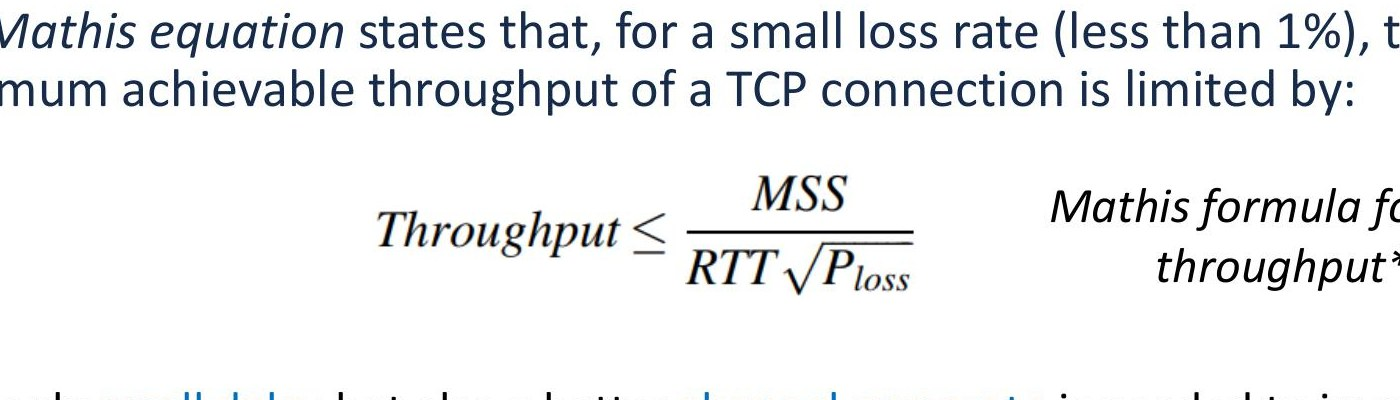
\includegraphics[keepaspectratio]{images/lezione-22-lab-multi-access-edge-computing-mec-img-01.jpg}}
\caption{La formula di Mathis: il throughput TCP è inversamente
proporzionale all'RTT e alla radice quadrata della probabilità di
perdita.}
\end{figure}

dove \(MSS\) è la \emph{Maximum Segment Size}, \(RTT\) è il
\emph{Round-Trip Time} e \(P_{loss}\) è la probabilità di perdita dei
pacchetti. La formula mostra come il throughput TCP sia limitato da due
fattori strettamente legati alla rete: non basta ridurre il ritardo, ma
serve anche migliorare il tasso di errore del canale. Questo motiva
l'adozione di meccanismi di \textbf{QoS} implementati come elaborazione
del traffico all'edge, finalizzati a ridurre la perdita di pacchetti.

\begin{callouttip}{Intuizione chiave}

Portare il server vicino all'utente riduce l'RTT; terminare il traffico
radio all'edge riduce anche \(P_{loss}\). Entrambi i fattori si
combinano per migliorare il throughput TCP in modo significativo.

\end{callouttip}

\subsection{La latenza nella pratica: misurazioni
reali}\label{la-latenza-nella-pratica-misurazioni-reali}

Un aspetto spesso controintuitivo è che la latenza end-to-end non è
necessariamente proporzionale alla distanza geografica. Misurazioni
effettuate in abitazioni distanti meno di 1 miglio quadrato mostrano
differenze enormi di latenza, specialmente quando sono coinvolti ISP
diversi.

I grafici CDF (Cumulative Distribution Function) illustrano il confronto
tra \emph{nearby cloudlet} (bordo della rete, scenario MEC) e
\emph{distant cloudlet} (cloud tradizionale) per tre diverse
applicazioni:

\begin{figure}
\centering
\pandocbounded{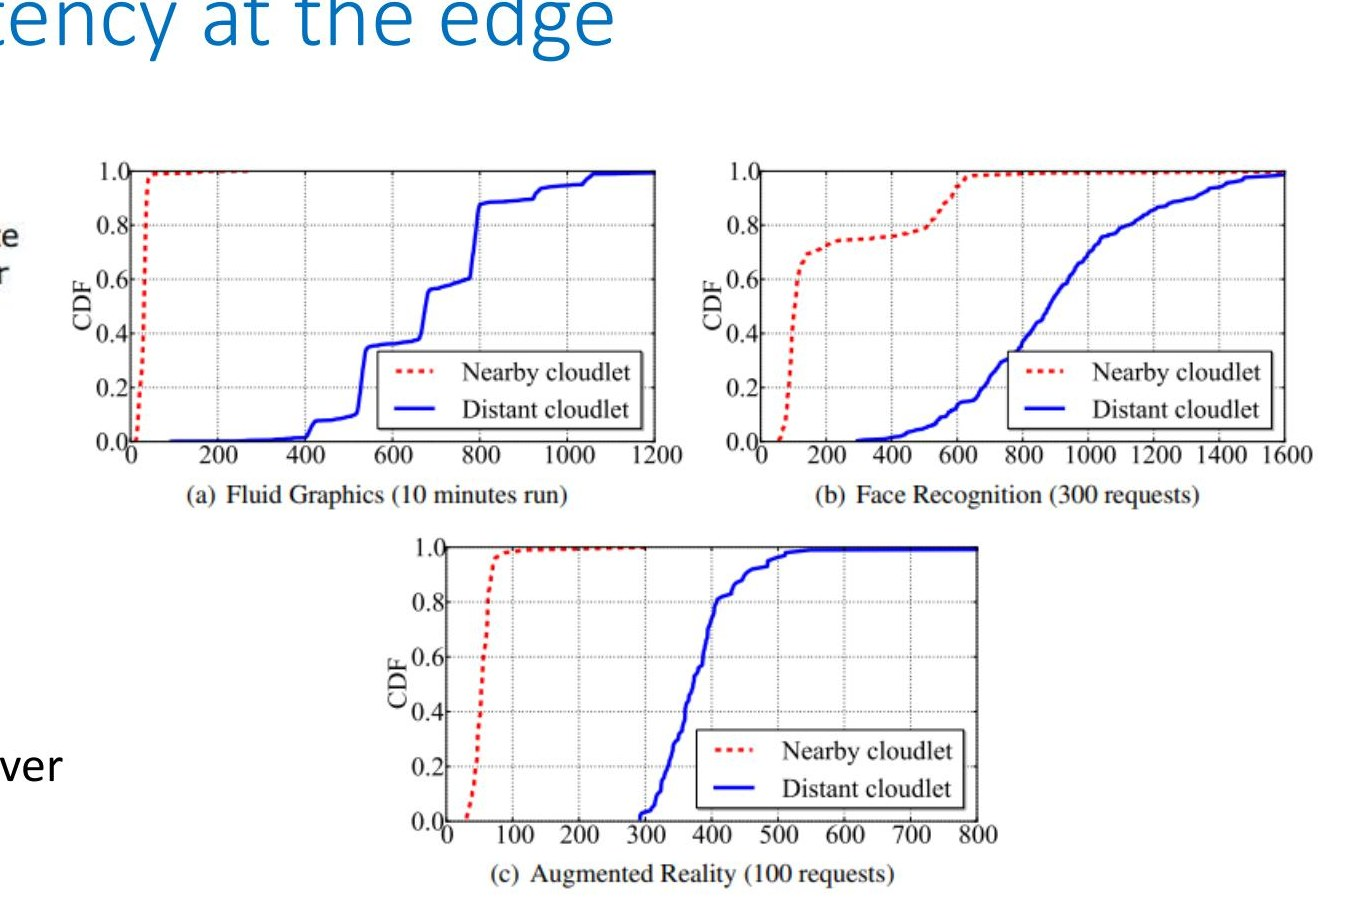
\includegraphics[keepaspectratio]{images/lezione-22-lab-multi-access-edge-computing-mec-img-02.jpg}}
\caption{CDF del tempo di risposta per Fluid Graphics, Face Recognition
e Augmented Reality: il cloudlet vicino (linea rossa tratteggiata)
mostra latenze significativamente inferiori.}
\end{figure}

\begin{calloutnote}{Evidenza empirica}

Il risultato chiave è che la latenza end-to-end dipende
dall'infrastruttura di rete (numero di hop, ISP attraversati) molto più
che dalla distanza fisica. Questo rende l'edge computing essenziale per
applicazioni sensibili alla latenza.

\end{calloutnote}

\begin{center}\rule{0.5\linewidth}{0.5pt}\end{center}

\section{MEC: definizione e standard}\label{mec-definizione-e-standard}

\textbf{ETSI MEC} (\emph{Multi-Access Edge Computing}) è il principale
standard internazionale nell'area dell'edge computing. La definizione
ufficiale ETSI recita:

\begin{calloutdefinition}{Multi-Access Edge Computing (MEC)}

MEC offre a sviluppatori di applicazioni e provider di contenuti
capacità di cloud computing e un ambiente di servizi IT al margine della
rete.

\end{calloutdefinition}

Il termine \textbf{``multi-access''} indica che lo standard è agnostico
rispetto alla tecnologia di accesso: è applicabile in linea di principio
a reti 4G/5G, Wi-Fi o accesso fisso. Il ``core business'' dello standard
ETSI MEC è la pubblicazione di \textbf{API standardizzate} che le
applicazioni virtualizzate all'edge possono utilizzare per accedere a
informazioni di rete.

\subsection{Standard di riferimento}\label{standard-di-riferimento}

Esistono due principali corpi di standardizzazione nel dominio dell'edge
computing:

{\def\LTcaptype{none} % do not increment counter
\begin{longtable}[]{@{}
  >{\raggedright\arraybackslash}p{(\linewidth - 4\tabcolsep) * \real{0.4167}}
  >{\raggedright\arraybackslash}p{(\linewidth - 4\tabcolsep) * \real{0.2917}}
  >{\raggedright\arraybackslash}p{(\linewidth - 4\tabcolsep) * \real{0.2917}}@{}}
\toprule\noalign{}
\begin{minipage}[b]{\linewidth}\raggedright
Standard
\end{minipage} & \begin{minipage}[b]{\linewidth}\raggedright
Focus
\end{minipage} & \begin{minipage}[b]{\linewidth}\raggedright
Note
\end{minipage} \\
\midrule\noalign{}
\endhead
\bottomrule\noalign{}
\endlastfoot
\textbf{ETSI MEC} & Edge computing da prospettiva IT, access-agnostic &
Definisce le API e le specifiche per piattaforme MEC \\
\textbf{3GPP} & Tecnologie radio e core network & Integra edge computing
dal Release 15 (5G) in poi \\
\end{longtable}
}

\begin{center}\rule{0.5\linewidth}{0.5pt}\end{center}

\section{Il concetto di ``edge'': dove si
trova?}\label{il-concetto-di-edge-dove-si-trova}

Il concetto di \emph{edge} non è definito in modo rigido dallo standard
ETSI, proprio per poter includere molte opzioni di deployment basate su
requisiti diversi (costi, traffico, presenza di utenti, tariffe). L'edge
può essere:

\begin{itemize}
\tightlist
\item
  \textbf{Base Station} (stazione radio base)
\item
  \textbf{WiFi Access Point}
\item
  \textbf{Data center} o micro-data center a uffici centrali, siti di
  aggregazione
\item
  \textbf{Locali del cliente} (\emph{customer premises})
\end{itemize}

\begin{figure}
\centering
\pandocbounded{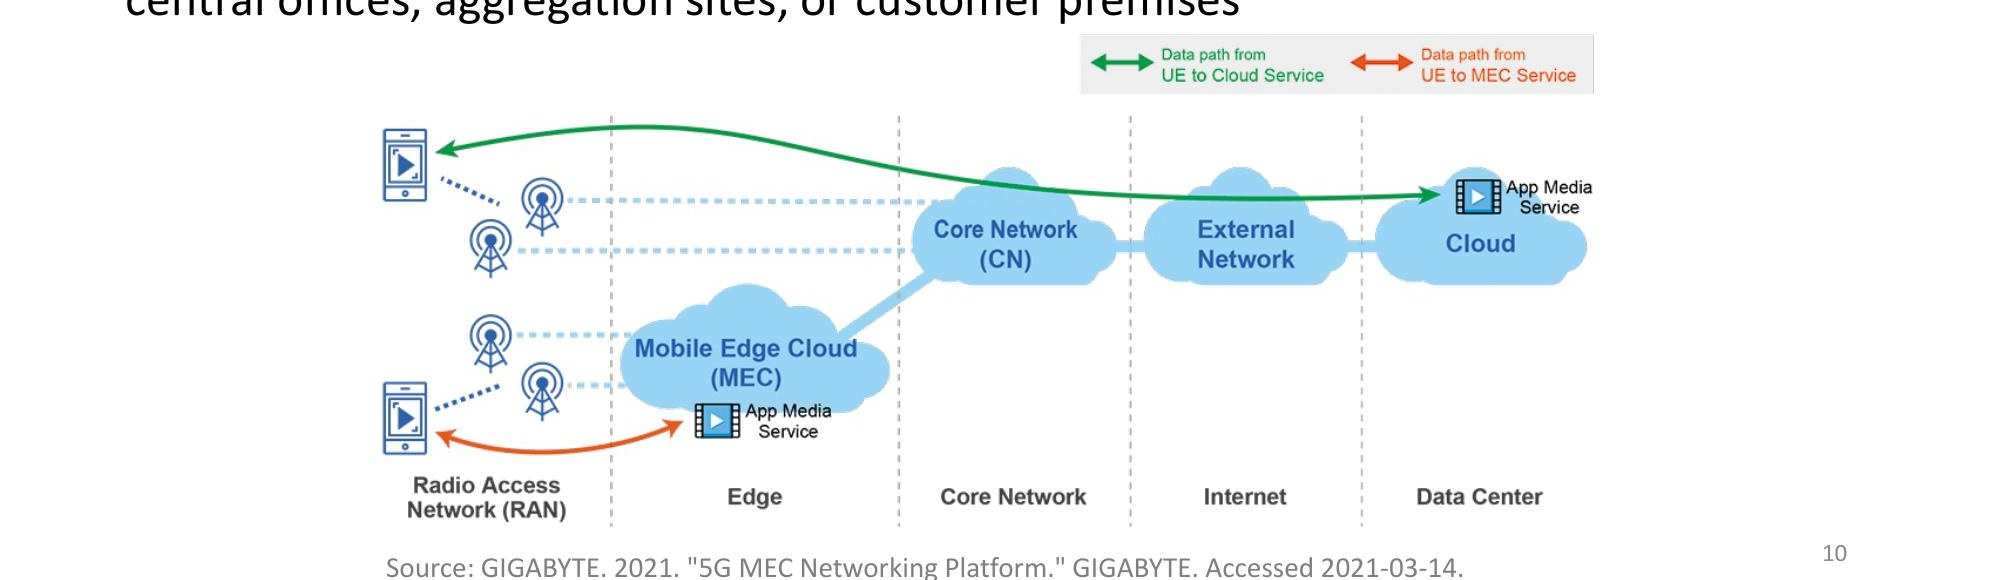
\includegraphics[keepaspectratio]{images/lezione-22-lab-multi-access-edge-computing-mec-img-03.jpg}}
\caption{Confronto tra il percorso dati UE→Cloud (verde, attraverso core
network, internet e data center) e UE→MEC Service (arancione, terminato
al Mobile Edge Cloud). Fonte: GIGABYTE, 2021.}
\end{figure}

\begin{center}\rule{0.5\linewidth}{0.5pt}\end{center}

\section{Benefici di MEC}\label{benefici-di-mec}

I due abilitatori chiave forniti da MEC sono:

\begin{enumerate}
\def\labelenumi{\arabic{enumi}.}
\tightlist
\item
  \textbf{Prossimità agli utenti finali}: riduzione della latenza
  end-to-end a livello del piano utente (UP -- \emph{User Plane}).
\item
  \textbf{Accesso alle informazioni radio locali} (piano di controllo,
  CP -- \emph{Control Plane}): permette di implementare meccanismi per
  migliorare il tasso di errore del canale.
\end{enumerate}

A questi si aggiungono benefici supplementari:

\begin{itemize}
\tightlist
\item
  possibilità di eseguire elaborazioni locali sfruttando grandi quantità
  di dati locali (sensori, dispositivi);
\item
  supporto al \textbf{task offloading} da dispositivi finali con
  capacità di elaborazione limitata;
\item
  facilitazione delle garanzie di \textbf{sicurezza e privacy}, ad
  esempio anonimizzando informazioni personali all'edge e trasmettendo
  solo dati aggregati al cloud centrale.
\end{itemize}

\begin{center}\rule{0.5\linewidth}{0.5pt}\end{center}

\section{Scenari di servizio MEC}\label{scenari-di-servizio-mec}

\subsection{Analisi di flussi video}\label{analisi-di-flussi-video}

Un caso d'uso emblematico è il sistema di monitoraggio video con
algoritmi di riconoscimento immagini, ad esempio per il riconoscimento
di targhe o il controllo degli accessi in aree urbane.

\begin{figure}
\centering
\pandocbounded{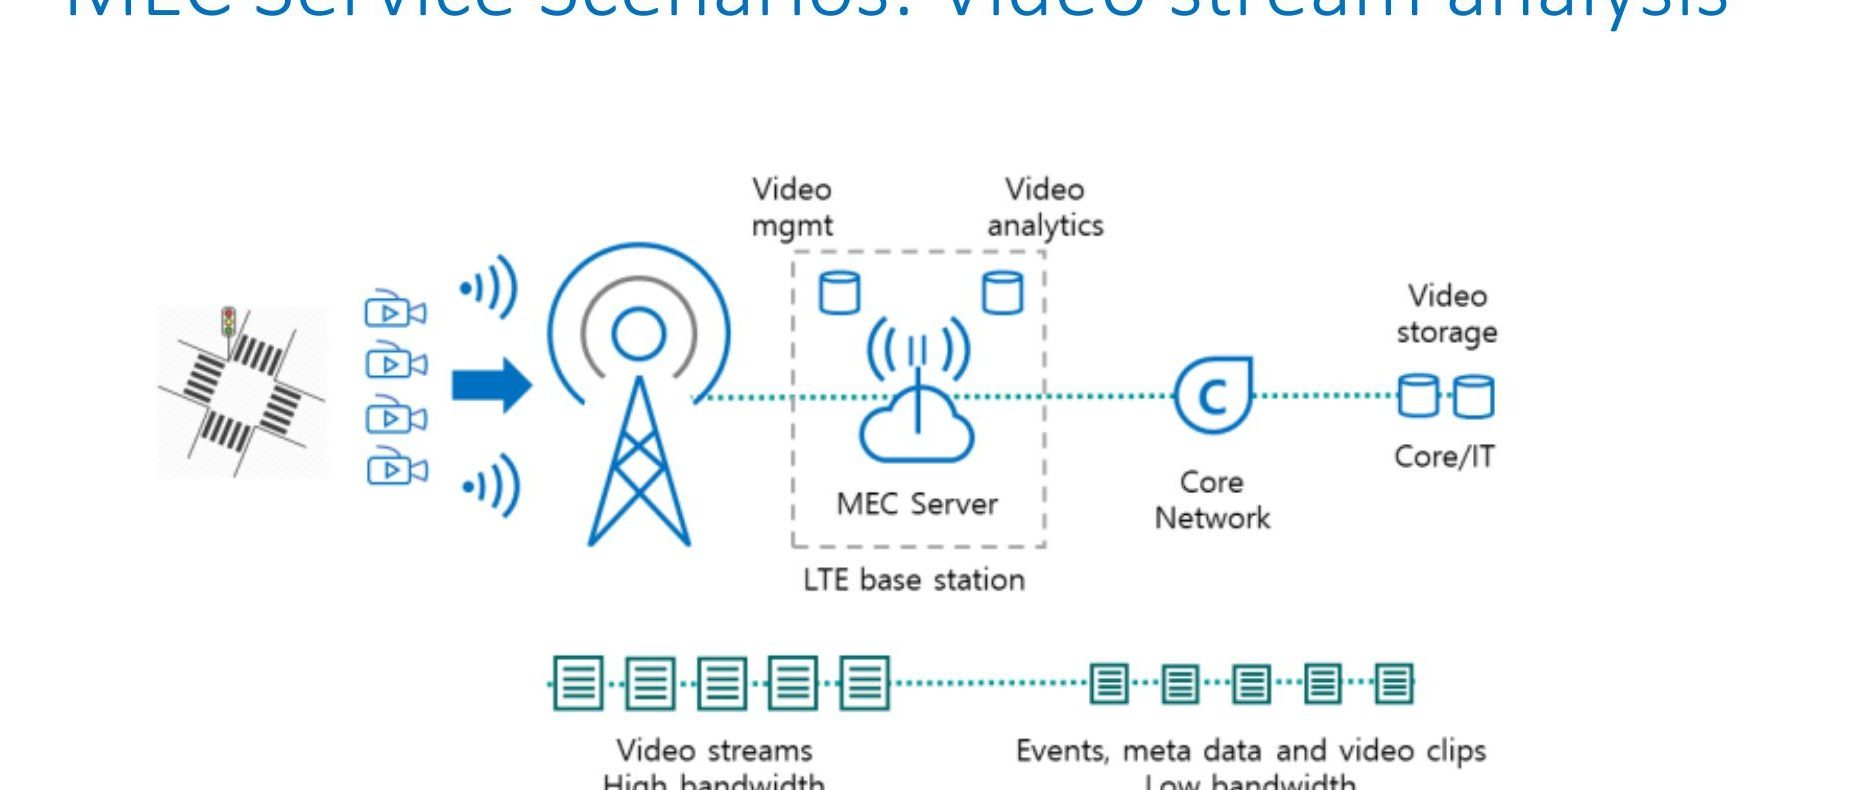
\includegraphics[keepaspectratio]{images/lezione-22-lab-multi-access-edge-computing-mec-img-04.jpg}}
\caption{Il MEC Server, co-locato con la base LTE, esegue video
management e analytics localmente. Verso la core network vengono
trasmessi solo eventi, metadati e clip rilevanti (bassa banda), anziché
stream video ad alta banda.}
\end{figure}

Eseguire il video analytics sul \textbf{MEC host} consente di: - evitare
la trasmissione di stream video ad alta banda attraverso la core network
verso servizi cloud remoti; - inviare alla rete solo i dati estratti
dall'elaborazione (risultati, metadati, clip rilevanti); - ottenere
prestazioni migliori rispetto sia a processare il video sulle telecamere
stesse sia a processarlo su un server remoto.

\subsection{IoT Gateway}\label{iot-gateway}

MEC può fungere da \textbf{gateway IoT} intelligente, aggregando il
traffico proveniente da dispositivi eterogenei (veicoli, sensori,
attuatori industriali, dispositivi consumer) e applicando analytics
verticali prima di trasmettere dati verso la core network e Internet.

\begin{figure}
\centering
\pandocbounded{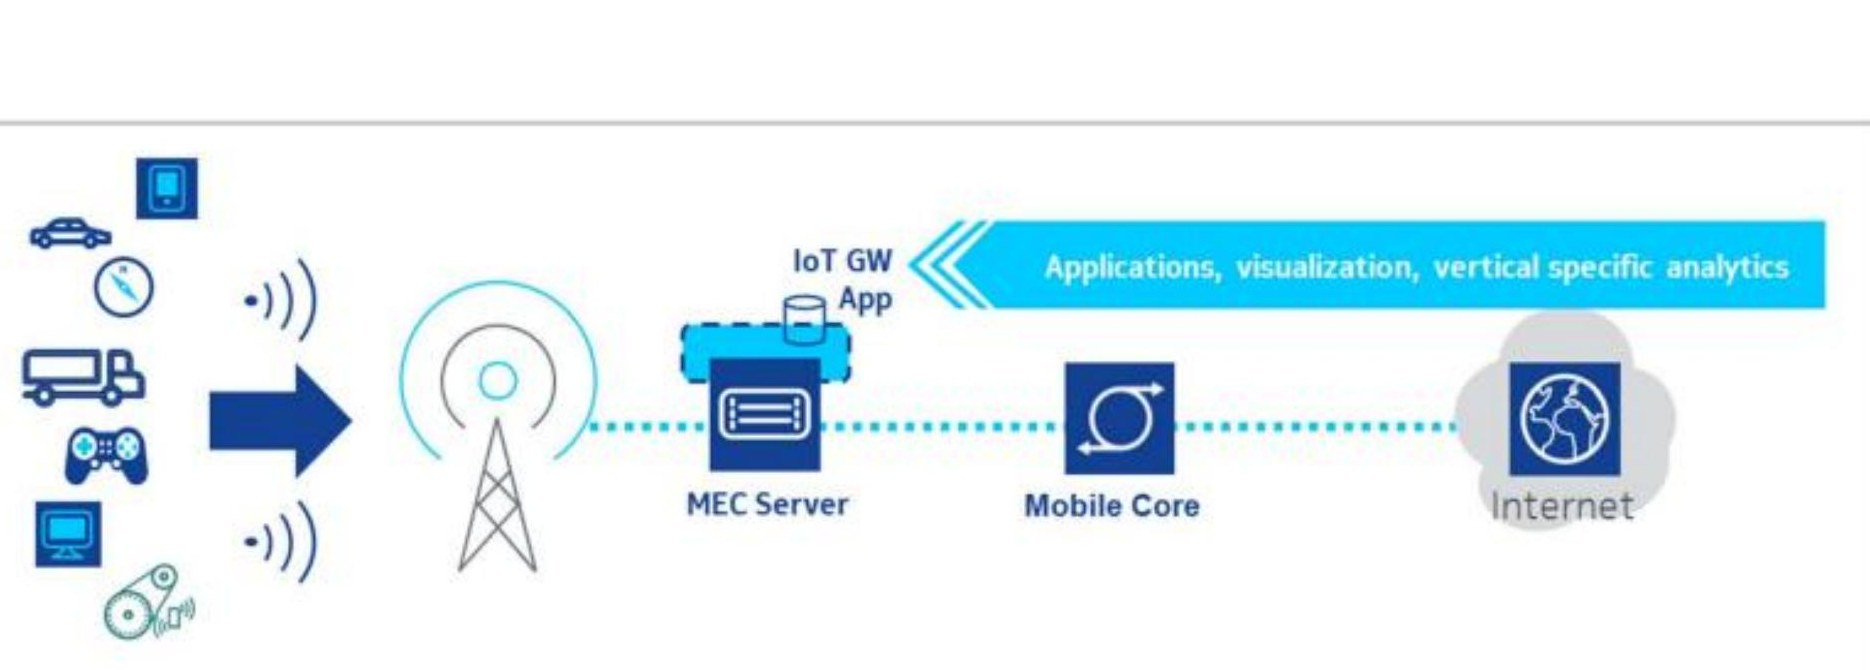
\includegraphics[keepaspectratio]{images/lezione-22-lab-multi-access-edge-computing-mec-img-05.jpg}}
\caption{Un'applicazione IoT GW App gira sul MEC Server, raccogliendo
traffico da dispositivi IoT eterogenei via radio. Verso la core network
vengono propagate solo analisi aggregate e eventi rilevanti.}
\end{figure}

\begin{center}\rule{0.5\linewidth}{0.5pt}\end{center}

\section{Architettura MEC}\label{architettura-mec}

\subsection{Il sistema MEC}\label{il-sistema-mec}

Un \textbf{sistema MEC} include i MEC host e la gestione MEC necessaria
per eseguire applicazioni MEC all'interno di una rete operatore.

\subsection{Il MEC Framework}\label{il-mec-framework}

\begin{figure}
\centering
\pandocbounded{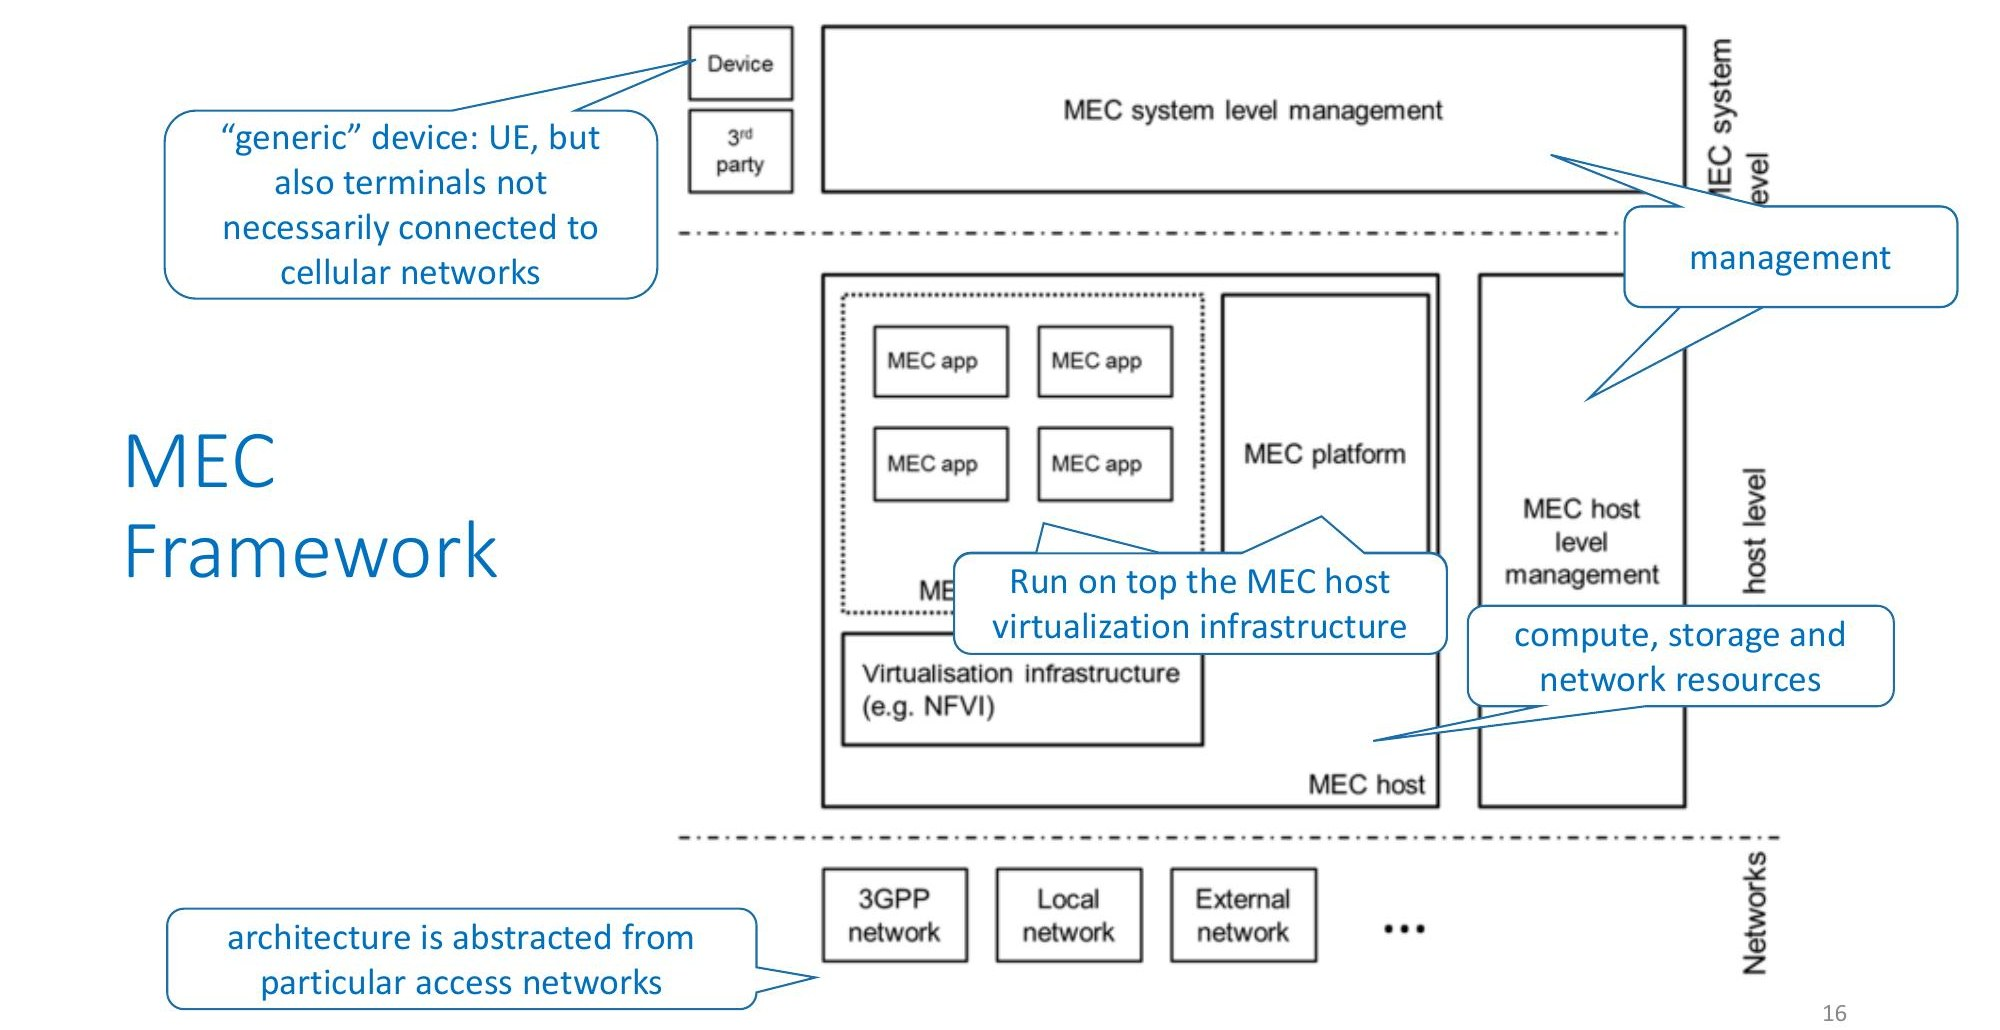
\includegraphics[keepaspectratio]{images/lezione-22-lab-multi-access-edge-computing-mec-img-06.jpg}}
\caption{Il MEC Framework: i MEC host ospitano la virtualization
infrastructure (NFV) con le MEC app e la MEC platform. La gestione è
strutturata su due livelli: system-level e host-level.}
\end{figure}

I componenti principali dell'architettura sono:

\begin{calloutdefinition}{MEC Host}

Include una \textbf{MEC platform} e una \textbf{virtualization
infrastructure} che fornisce risorse di calcolo, storage e rete per le
MEC application. È il server fisico che ospita la piattaforma e le
applicazioni.

\end{calloutdefinition}

\begin{calloutdefinition}{MEC Platform}

Raccolta delle funzionalità essenziali per eseguire le MEC application
su una particolare infrastruttura di virtualizzazione, abilitandole a
consumare e offrire \textbf{MEC services}. La piattaforma può essa
stessa offrire servizi.

\end{calloutdefinition}

\begin{calloutdefinition}{MEC Application}

Applicazione che gira sopra la virtualization infrastructure fornita dal
MEC host. Può interagire con la MEC platform per consumare e fornire MEC
services.

\end{calloutdefinition}

\begin{calloutdefinition}{MEC Management}

Divisa in \emph{system-level} e \emph{host-level}, gestisce
l'orchestrazione dell'intero sistema MEC.

\end{calloutdefinition}

L'architettura è volutamente \textbf{astratta dalla tecnologia di
accesso specifica}: le reti sottostanti possono essere 3GPP (4G/5G),
Wi-Fi, rete fissa o qualsiasi combinazione. I dispositivi terminali non
sono necessariamente UE cellulari, ma qualsiasi terminale connesso
all'infrastruttura d'accesso.

\begin{center}\rule{0.5\linewidth}{0.5pt}\end{center}

\section{Categorie di casi d'uso}\label{categorie-di-casi-duso}

I casi d'uso MEC si raggruppano in tre categorie principali:

{\def\LTcaptype{none} % do not increment counter
\begin{longtable}[]{@{}
  >{\raggedright\arraybackslash}p{(\linewidth - 2\tabcolsep) * \real{0.5789}}
  >{\raggedright\arraybackslash}p{(\linewidth - 2\tabcolsep) * \real{0.4211}}@{}}
\toprule\noalign{}
\begin{minipage}[b]{\linewidth}\raggedright
Categoria
\end{minipage} & \begin{minipage}[b]{\linewidth}\raggedright
Esempi
\end{minipage} \\
\midrule\noalign{}
\endhead
\bottomrule\noalign{}
\endlastfoot
\textbf{Consumer-oriented services} & Gaming, remote desktop, assistenza
cognitiva, servizi in tempo reale per stadi/retail, offloading
computazionale \\
\textbf{Operator and third-party services} & Tracciamento posizione
dispositivi, big data, video analytics, veicoli connessi, sicurezza \\
\textbf{Network performance \& QoE improvements} & Content/DNS caching,
ottimizzazione prestazioni, ottimizzazione e accelerazione video \\
\end{longtable}
}

\begin{center}\rule{0.5\linewidth}{0.5pt}\end{center}

\section{MEC Service APIs}\label{mec-service-apis}

MEC standardizza un insieme di \textbf{API di servizio} che consentono
alle applicazioni virtualizzate all'edge di accedere a informazioni di
rete e utente dal nodo locale. Le API principali sono:

{\def\LTcaptype{none} % do not increment counter
\begin{longtable}[]{@{}
  >{\raggedright\arraybackslash}p{(\linewidth - 2\tabcolsep) * \real{0.2778}}
  >{\raggedright\arraybackslash}p{(\linewidth - 2\tabcolsep) * \real{0.7222}}@{}}
\toprule\noalign{}
\begin{minipage}[b]{\linewidth}\raggedright
API
\end{minipage} & \begin{minipage}[b]{\linewidth}\raggedright
Funzionalità
\end{minipage} \\
\midrule\noalign{}
\endhead
\bottomrule\noalign{}
\endlastfoot
\textbf{Radio Network Info API (RNIS)} & Condizioni radio attuali, Cell
ID, intensità segnale, bearer UE \\
\textbf{Location API} & Posizione geografica/logica degli UE, lista UE
in un'area, movimenti in/out \\
\textbf{UE Identity API} & Identificazione dei terminali \\
\textbf{Bandwidth Management API} & Gestione della banda \\
\textbf{App Lifecycle Management API} & Ciclo di vita delle
applicazioni \\
\textbf{WLAN Info API} & Informazioni sulle reti Wi-Fi \\
\textbf{V2X Info Service API} & Comunicazioni vehicle-to-everything \\
\textbf{Service Discovery API} & Scoperta dei servizi disponibili \\
\textbf{Mobility API} & Gestione della continuità di servizio durante la
mobilità \\
\textbf{MultiAccess Traffic Steering API} & Steering, splitting e
duplicazione del traffico su accessi multipli \\
\end{longtable}
}

\subsection{Radio Network Information API
(RNIS)}\label{radio-network-information-api-rnis}

La RNIS fornisce informazioni aggiornate sulle condizioni radio: Cell
ID, intensità del segnale, misurazioni relative al piano utente,
contesto degli UE connessi ai nodi radio associati al MEC host. È utile
sia per le MEC app che vogliono ottimizzare i propri servizi (ad esempio
guidare il throughput video adattativamente) sia per la MEC platform per
ottimizzare le procedure di mobilità.

\subsection{Location API}\label{location-api}

La Location API espone informazioni di localizzazione con due tipi di
rappresentazione: - \textbf{Geolocalizzazione}: coordinate geografiche
GPS. - \textbf{Localizzazione logica}: Cell ID, identificativi di
settore radio.

Le informazioni includono: posizione di UE specifici, lista degli UE in
un'area geografica, notifiche di ingresso/uscita da un'area, posizione
dei nodi radio associati all'host.

\begin{center}\rule{0.5\linewidth}{0.5pt}\end{center}

\section{MultiAccess Traffic Steering (MTS)
API}\label{multiaccess-traffic-steering-mts-api}

Nessuna singola tecnologia di accesso wireless è in grado di soddisfare
simultaneamente tutti i requisiti di comunicazione umana e machine-type:
massima velocità di trasmissione da un lato, massima affidabilità
dall'altro. La \textbf{MTS API} nasce per sfruttare la presenza di
connessioni multiple combinandole intelligentemente.

\subsection{Il trade-off fondamentale}\label{il-trade-off-fondamentale}

L'idea di base è semplice: se si dispone di \(N\) link wireless,
ciascuno con data rate \(R\) Mbps e affidabilità \(p\), combinando i
link si può ottenere:

\begin{itemize}
\tightlist
\item
  \textbf{Split traffic} (traffico suddiviso): data rate aggregato
  \(N    imes R\) Mbps, stessa affidabilità \(p\) --- si guadagna in
  throughput ma non in affidabilità.
\item
  \textbf{Duplicate traffic} (traffico duplicato): stesso data rate
  \(R\), affidabilità \(p^N\) --- si guadagna in affidabilità ma non in
  throughput.
\end{itemize}

\begin{calloutwarning}{Trade-off esclusivo}

Il miglioramento del data rate e il miglioramento dell'affidabilità non
si ottengono contemporaneamente. Le due strategie (split e duplicate)
sono mutuamente esclusive in termini di beneficio primario.

\end{calloutwarning}

La tabella seguente mostra un esempio numerico con \(N\) link da 100
Mbps e affidabilità \(10^{-3}\):

\begin{figure}
\centering
\pandocbounded{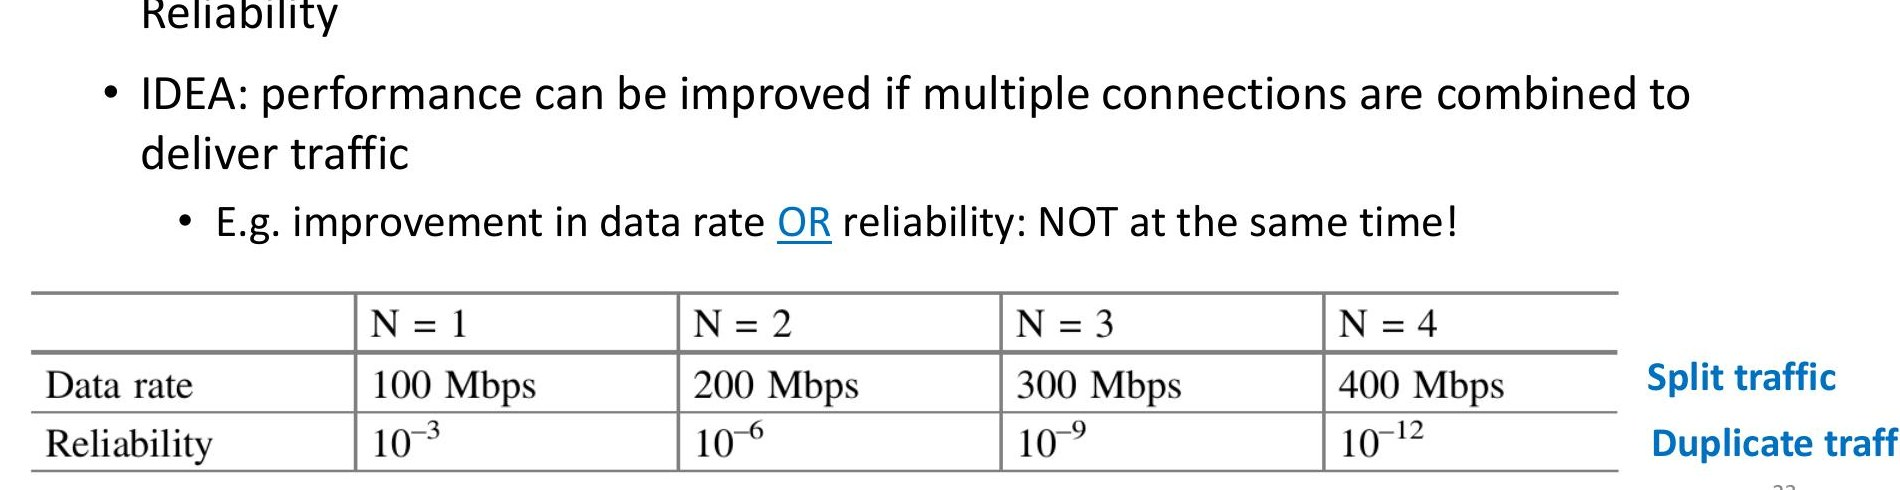
\includegraphics[keepaspectratio]{images/lezione-22-lab-multi-access-edge-computing-mec-img-07.jpg}}
\caption{Con N=4 link: data rate aggregato 400 Mbps (split) oppure
affidabilità \(10^{-12}\) (duplicate). Le due colonne ``Split traffic''
e ``Duplicate traffic'' evidenziano il trade-off.}
\end{figure}

\subsection{Operazioni MTS supportate}\label{operazioni-mts-supportate}

{\def\LTcaptype{none} % do not increment counter
\begin{longtable}[]{@{}
  >{\raggedright\arraybackslash}p{(\linewidth - 4\tabcolsep) * \real{0.3077}}
  >{\raggedright\arraybackslash}p{(\linewidth - 4\tabcolsep) * \real{0.2051}}
  >{\raggedright\arraybackslash}p{(\linewidth - 4\tabcolsep) * \real{0.4872}}@{}}
\toprule\noalign{}
\begin{minipage}[b]{\linewidth}\raggedright
Operazione
\end{minipage} & \begin{minipage}[b]{\linewidth}\raggedright
Logica
\end{minipage} & \begin{minipage}[b]{\linewidth}\raggedright
Caso d'uso tipico
\end{minipage} \\
\midrule\noalign{}
\endhead
\bottomrule\noalign{}
\endlastfoot
\textbf{Low Cost} & Usa la rete non misurata (Wi-Fi) quando disponibile
& Email, backup in background \\
\textbf{Low Latency} & Usa la connessione con latenza minore & Controllo
remoto, gaming \\
\textbf{High Throughput} & Usa la rete con throughput maggiore, o più
reti simultaneamente & Video streaming HD \\
\textbf{Redundancy} & Duplica i pacchetti su più connessioni & Controllo
robotico (URLLC) \\
\end{longtable}
}

\begin{callouttip}{Esempi pratici di MTS}

\begin{itemize}
\tightlist
\item
  \textbf{Email/Dropbox}: applicazione data-centric in background, non
  sensibile a latenza né throughput → preferisce Wi-Fi (Low Cost).
\item
  \textbf{Controllo robot} (URLLC): richiede altissima affidabilità e
  bassa latenza → Redundancy, pacchetti duplicati su più connessioni
  simultaneamente.
\item
  \textbf{Video HD real-time}: richiede alto throughput → High
  Throughput con bandwidth aggregation (traffic split su più link).
\end{itemize}

\end{callouttip}

\subsection{Esercizio: applicabilità
MTS}\label{esercizio-applicabilituxe0-mts}

\newpage

\chapter{Teoria dei Segnali: Introduzione e Serie di
Fourier}\label{teoria-dei-segnali-introduzione-e-serie-di-fourier}

\section{Perché la Teoria dei
Segnali?}\label{perchuxe9-la-teoria-dei-segnali}

I sistemi moderni --- reti mobili 4G/5G, dispositivi IoT, sistemi audio
--- elaborano \textbf{segnali} per rappresentare e trasmettere
informazione. Capire come questi segnali sono strutturati, come vengono
disturbati dal canale trasmissivo, e come possono essere analizzati e
trasformati è il fondamento dell'ingegneria delle comunicazioni
digitali.

La teoria dei segnali serve a quattro scopi pratici fondamentali. Il
primo è \textbf{estrarre informazione}: identificare frequenze, pattern
ed eventi rilevanti (es. riconoscimento vocale, analisi di segnali
biomedici). Il secondo è \textbf{rimuovere effetti indesiderati}:
filtrare il rumore, compensare distorsioni del canale, mitigare il
fading multipath nelle reti wireless. Il terzo è \textbf{trasmettere
efficientemente l'informazione}: codificare i segnali per il canale (es.
OFDM in 4G/5G che distribuisce i dati su più frequenze). Il quarto è
\textbf{abilitare l'elaborazione digitale}: convertire segnali analogici
in forma digitale tramite campionamento e quantizzazione.

\begin{figure}
\centering
\pandocbounded{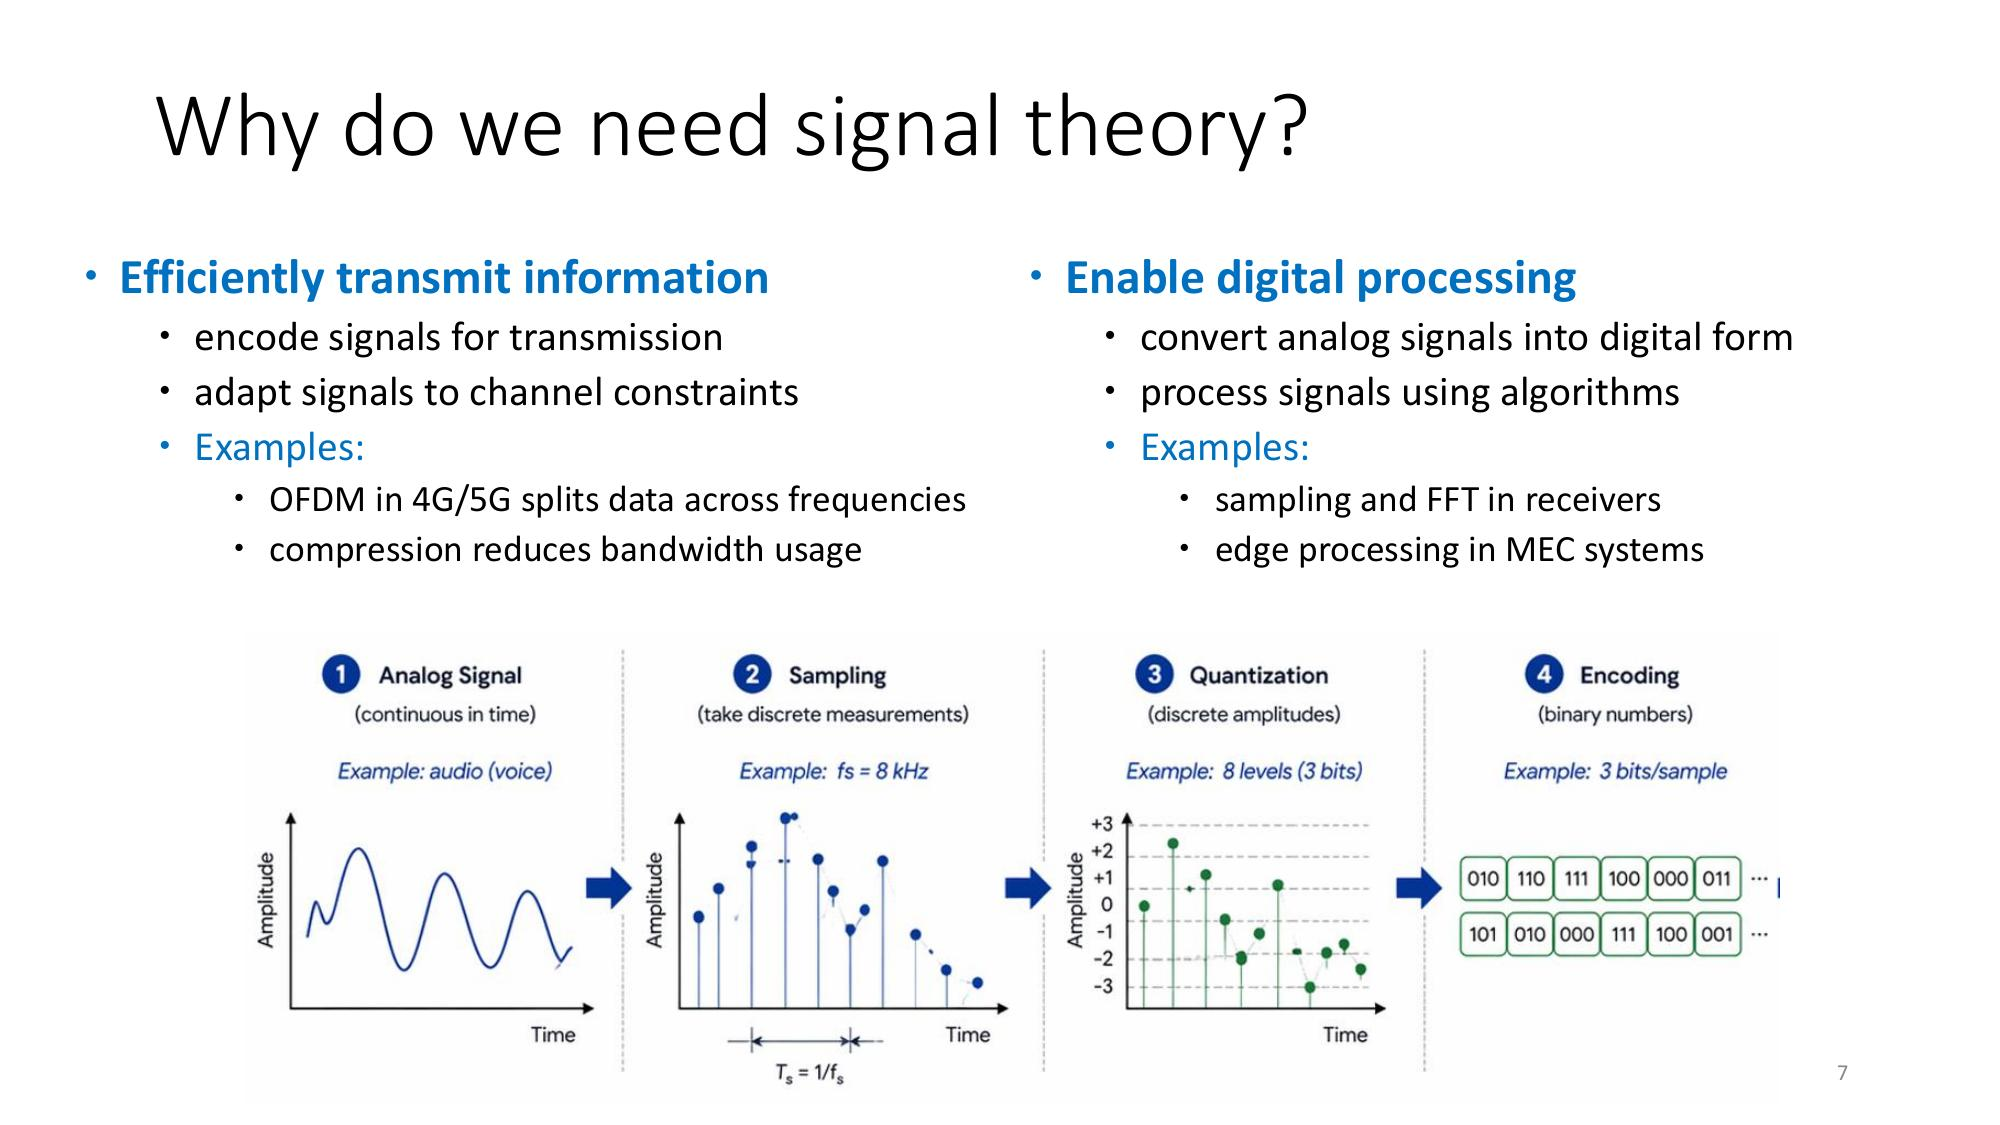
\includegraphics[keepaspectratio]{images/lezione-25-lab-teoria-dei-segnali-introduzione-e-serie-di-fourier-img-01.jpg}}
\caption{Dalla sorgente analogica ai bit: campionamento
(discretizzazione nel tempo), quantizzazione (discretizzazione
dell'ampiezza), codifica binaria.}
\end{figure}

\begin{center}\rule{0.5\linewidth}{0.5pt}\end{center}

\section{Classificazione dei Segnali}\label{classificazione-dei-segnali}

\begin{calloutdefinition}{Segnale}

Un segnale è una variazione di una grandezza fisica che porta
informazione. Formalmente è una funzione
\(f(t): \mathfrak{D} \longrightarrow \mathfrak{C}\) dove il dominio
\(\mathfrak{D}\) può essere \(\mathbb{R}\) (tempo continuo) o
\(\mathbb{Z}\) (tempo discreto), e il codominio \(\mathfrak{C}\) può
essere \(\mathbb{R}\) (ampiezza continua) o un insieme discreto
(ampiezza quantizzata).

\end{calloutdefinition}

Ci concentriamo su \textbf{segnali deterministici monodimensionali}: la
variabile indipendente è il tempo, e il segnale è noto prima di essere
prodotto (al contrario dei segnali aleatori, analizzati con metodi
probabilistici).

\subsection{Segnali a Tempo Continuo}\label{segnali-a-tempo-continuo}

Quando il dominio è \(\mathbb{R}\), il segnale è detto
\textbf{analogico} (\emph{analog}). Se anche il codominio è
\(\mathbb{R}\), l'ampiezza è continua; se il codominio è un insieme
discreto (es. \(\mathbb{Z}\)), l'ampiezza è quantizzata.

\begin{figure}
\centering
\pandocbounded{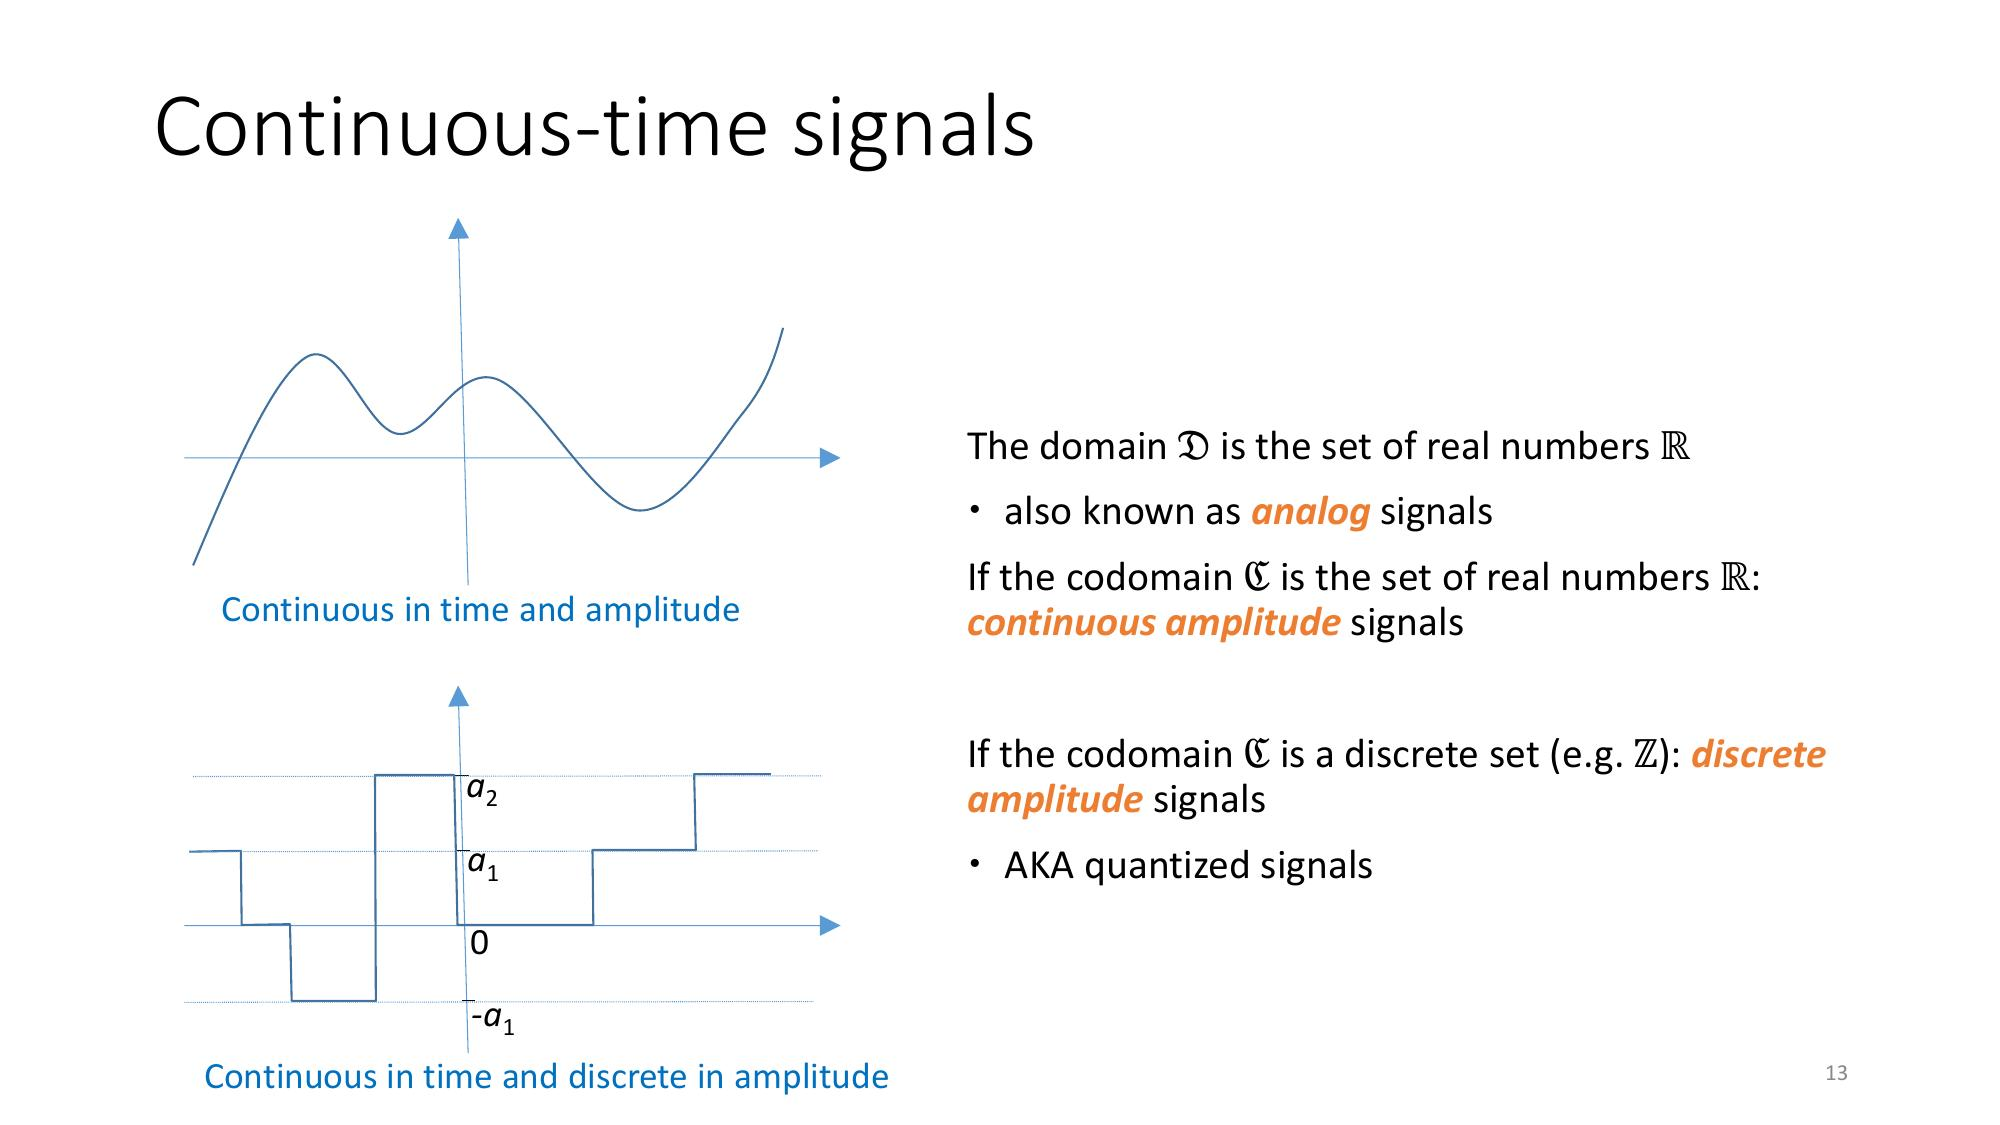
\includegraphics[keepaspectratio]{images/lezione-25-lab-teoria-dei-segnali-introduzione-e-serie-di-fourier-img-02.jpg}}
\caption{In alto: segnale analogico, continuo in tempo e ampiezza. In
basso: segnale continuo in tempo ma quantizzato in ampiezza (segnale a
gradini).}
\end{figure}

\subsection{Segnali a Tempo Discreto}\label{segnali-a-tempo-discreto}

Quando il dominio è
\(\mathbb{Z}(T) = \{nT, \forall n \in \mathbb{Z}, T \in \mathbb{R}\}\),
il segnale è detto \textbf{discreto}. Ad esempio
\(\mathbb{Z}(2) = \{\ldots, -4, -2, 0, 2, 4, \ldots\}\). Un segnale
discreto con ampiezza presa da un insieme finito di simboli è detto
\textbf{digitale} (\emph{digital}), o sequenza simbolica.

\begin{figure}
\centering
\pandocbounded{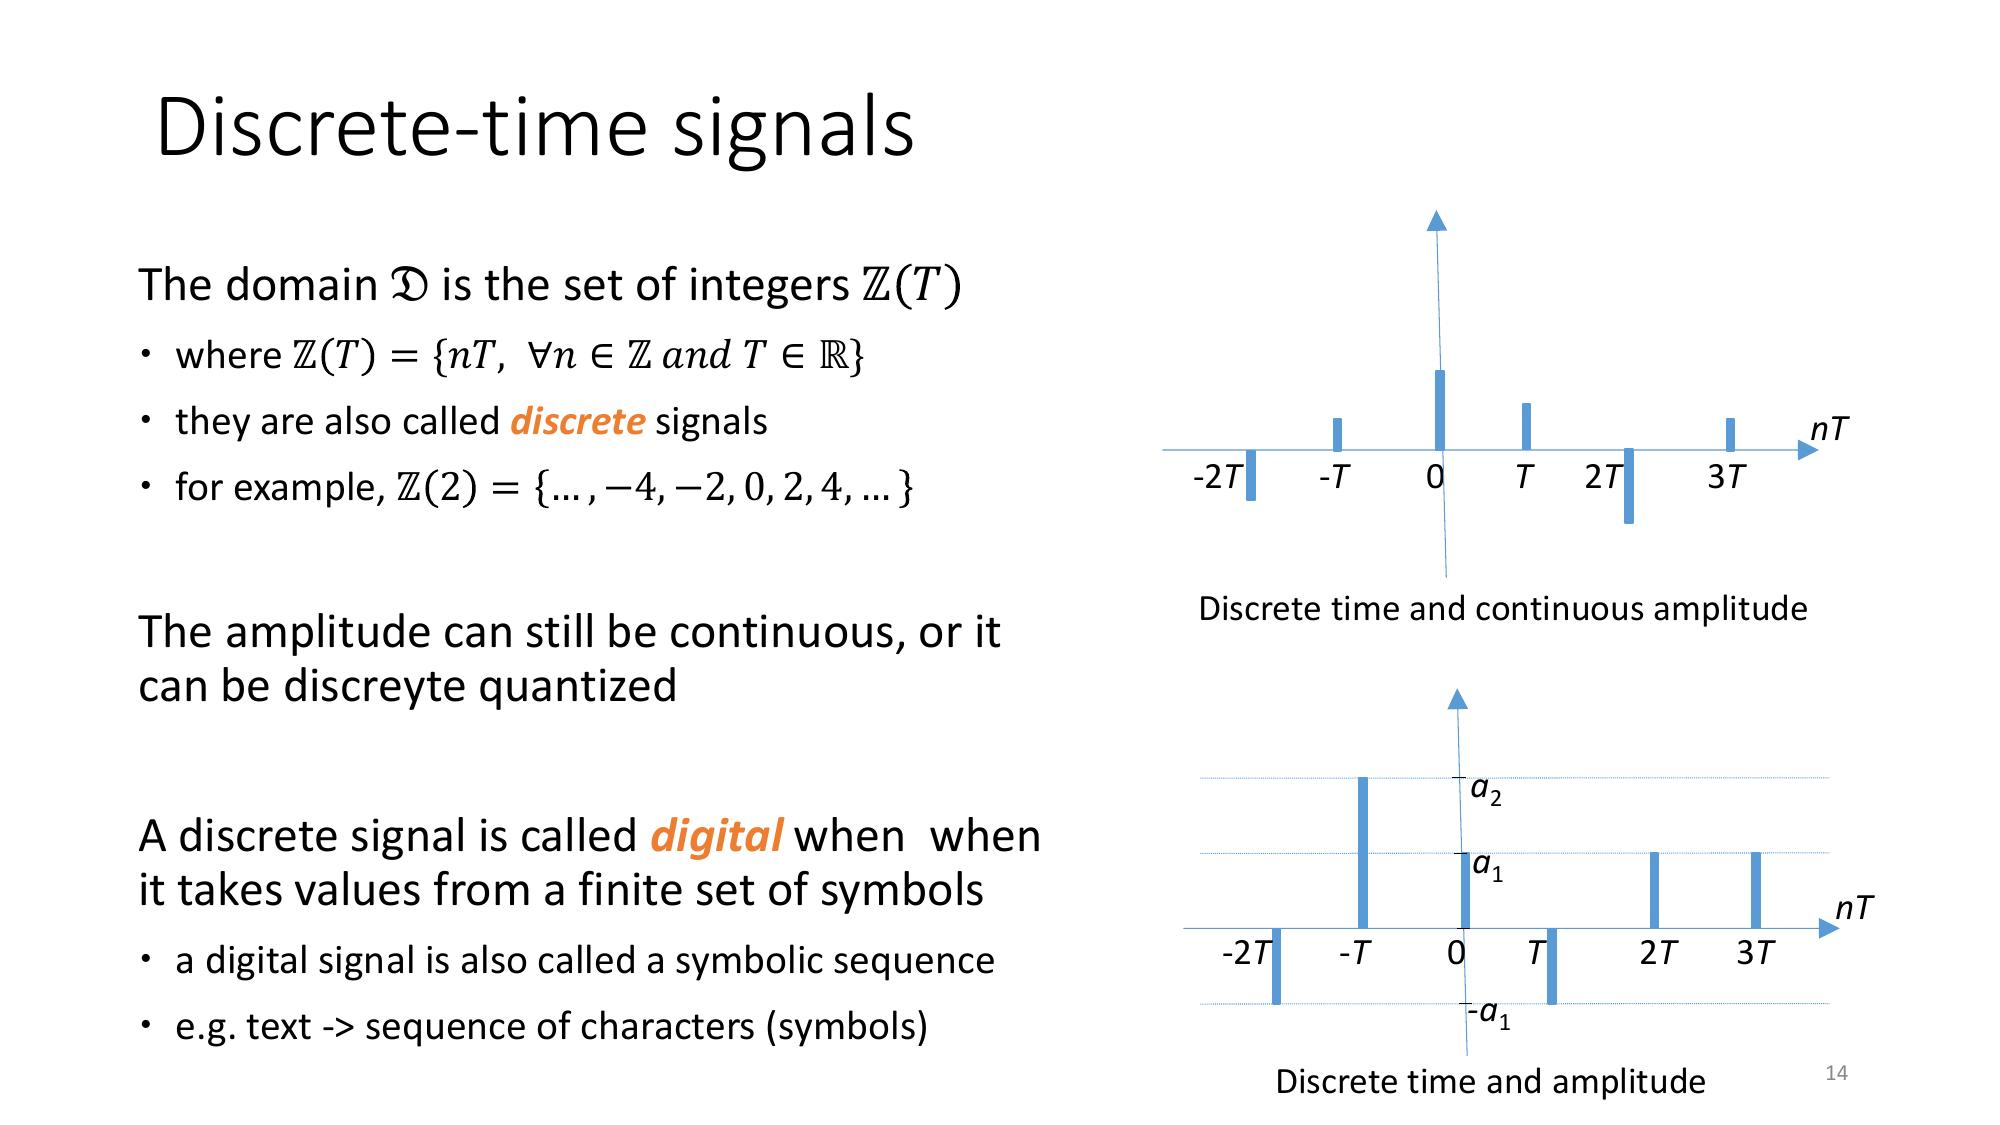
\includegraphics[keepaspectratio]{images/lezione-25-lab-teoria-dei-segnali-introduzione-e-serie-di-fourier-img-03.jpg}}
\caption{In alto: segnale discreto con ampiezza continua. In basso:
segnale digitale, discreto sia nel tempo che nell'ampiezza.}
\end{figure}

\subsection{Tabella Riepilogativa}\label{tabella-riepilogativa}

{\def\LTcaptype{none} % do not increment counter
\begin{longtable}[]{@{}
  >{\raggedright\arraybackslash}p{(\linewidth - 4\tabcolsep) * \real{0.3333}}
  >{\raggedright\arraybackslash}p{(\linewidth - 4\tabcolsep) * \real{0.3333}}
  >{\raggedright\arraybackslash}p{(\linewidth - 4\tabcolsep) * \real{0.3333}}@{}}
\toprule\noalign{}
\begin{minipage}[b]{\linewidth}\raggedright
Tempo
\end{minipage} & \begin{minipage}[b]{\linewidth}\raggedright
Ampiezza
\end{minipage} & \begin{minipage}[b]{\linewidth}\raggedright
Tipo
\end{minipage} \\
\midrule\noalign{}
\endhead
\bottomrule\noalign{}
\endlastfoot
Continuo (\(\mathbb{R}\)) & Continua (\(\mathbb{R}\)) & Segnale
analogico \\
Continuo (\(\mathbb{R}\)) & Discreta (\(\mathbb{Z}\)) & Segnale
quantizzato \\
Discreto (\(\mathbb{Z}(T)\)) & Continua (\(\mathbb{R}\)) & Segnale
discreto \\
Discreto (\(\mathbb{Z}(T)\)) & Discreta (insieme finito) & Segnale
digitale \\
\end{longtable}
}

\subsection{Bitrate di una Sorgente
Digitale}\label{bitrate-di-una-sorgente-digitale}

Quando un segnale analogico viene convertito in digitale con frequenza
di campionamento \(f_c\) campioni/secondo e ogni campione è codificato
con \(M\) bit:

\[\text{Bitrate} = f_c \cdot M \quad [\text{bit/secondo}]\]

Maggiori \(f_c\) e \(M\) producono migliore fedeltà ma richiedono
maggiore capacità trasmissiva.

\begin{center}\rule{0.5\linewidth}{0.5pt}\end{center}

\section{Trasmissione e Canale}\label{trasmissione-e-canale}

\subsection{Il Modello del Canale}\label{il-modello-del-canale}

Nella trasmissione di informazione, un trasduttore alla sorgente
converte un messaggio in un segnale fisico (es. un'antenna converte
energia elettrica in onde elettromagnetiche), il segnale si propaga
attraverso il mezzo, e un trasduttore alla destinazione converte il
segnale di ritorno in messaggio. Il \textbf{canale} non è un mezzo
ideale: agisce come un sistema che modifica il segnale.

Le principali forme di degrado sono la \textbf{distorsione} (variazione
della forma d'onda, es. attenuazione differenziata per frequenza), la
\textbf{propagazione multipath} (il segnale raggiunge il ricevitore
attraverso percorsi multipli con ritardi diversi, causando
interferenza), e il \textbf{rumore} (segnale indesiderato sovrapposto a
quello utile).

\begin{calloutdefinition}{SNR — Signal-to-Noise Ratio}

Il rapporto segnale-rumore misura la qualità del segnale ricevuto
rispetto al rumore di fondo:
\[SNR_{dB} = 10 \log_{10} \frac{P_{signal}}{P_{noise}}\]

\end{calloutdefinition}

\subsection{Teorema di Shannon}\label{teorema-di-shannon}

Il risultato fondamentale della teoria dell'informazione stabilisce la
capacità massima di un canale:

\[C = B \log_2 (1 + SNR)\]

dove \(B\) è la banda disponibile in Hz, \(SNR\) il rapporto
segnale-rumore, e \(C\) la capacità del canale in bit/secondo. Questo
crea un trade-off inevitabile: ridurre la distorsione di quantizzazione
alla sorgente aumenta la quantità di informazione da trasmettere, che
deve rientrare entro la capacità \(C\).

\begin{center}\rule{0.5\linewidth}{0.5pt}\end{center}

\section{Serie di Fourier: dal Tempo alla
Frequenza}\label{serie-di-fourier-dal-tempo-alla-frequenza}

\subsection{L'Intuizione Fondamentale}\label{lintuizione-fondamentale}

Un segnale periodico può essere visto come una sovrapposizione di
componenti sinusoidali, ciascuna con frequenza, ampiezza e fase
specifiche. Questo cambio di prospettiva --- dal dominio del tempo al
\textbf{dominio della frequenza} --- è cruciale perché il canale
trasmissivo agisce in modo diverso su componenti a frequenza diversa.
Per analizzare e predire tale comportamento, occorre identificare
esplicitamente le componenti frequenziali di un segnale.

La serie di Fourier decompone una funzione come somma di infinite
funzioni oscillanti a frequenze diverse. È formalmente un cambio di
coordinate: dal dominio del tempo a quello della frequenza. La base di
questa decomposizione è un insieme di funzioni \(\varphi_n(t)\)
ortogonali, analogamente alla decomposizione di un vettore in uno spazio
vettoriale.

\begin{figure}
\centering
\pandocbounded{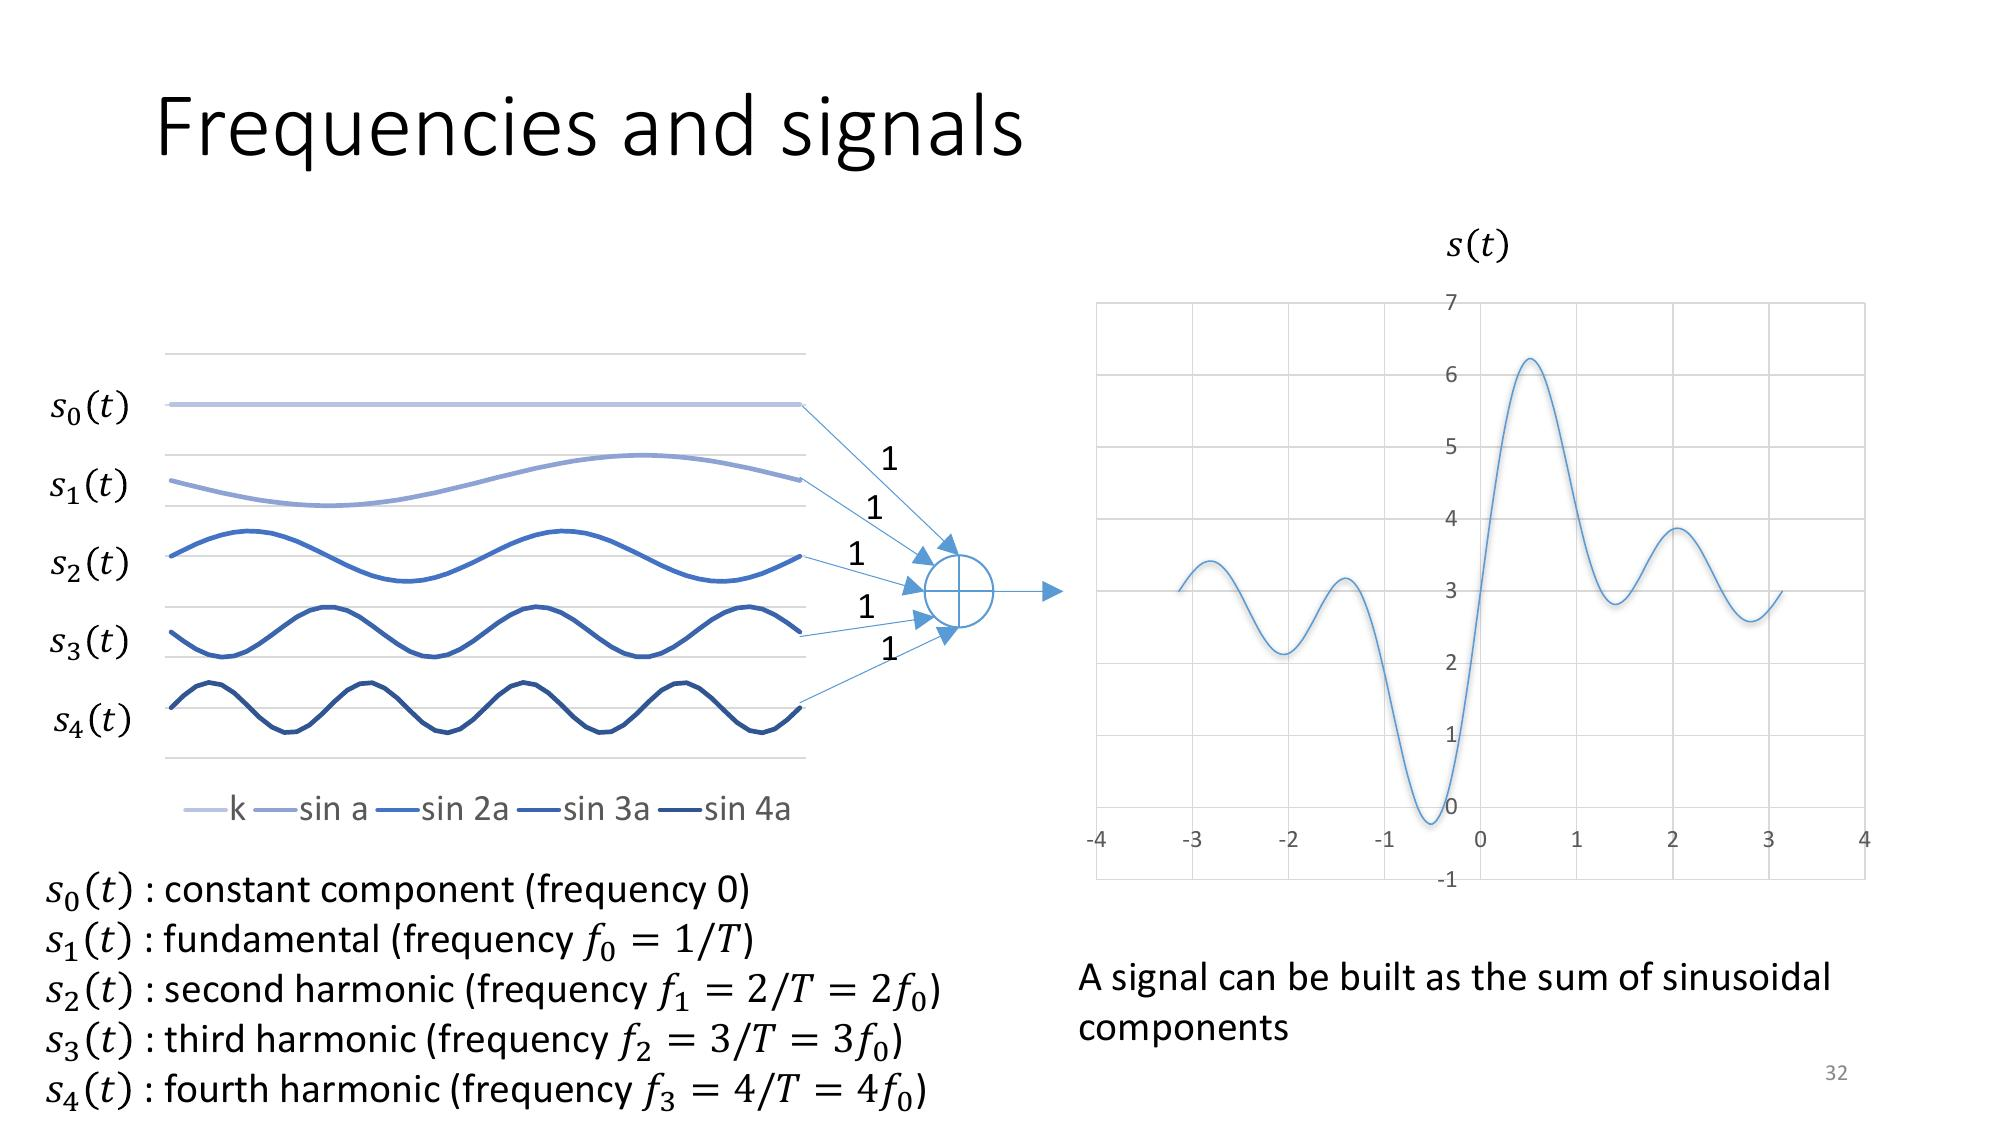
\includegraphics[keepaspectratio]{images/lezione-25-lab-teoria-dei-segnali-introduzione-e-serie-di-fourier-img-04.jpg}}
\caption{Un segnale si costruisce sommando componenti sinusoidali: la
componente costante (\(s_0\)), la fondamentale (\(s_1\)) e le armoniche
superiori (\(s_2, s_3, s_4\)). Cambiare i coefficienti cambia il segnale
risultante.}
\end{figure}

\subsection{Segnali Periodici
Continui}\label{segnali-periodici-continui}

Un segnale continuo \(s(t): \mathbb{R} \to \mathbb{R}\) è
\textbf{periodico con periodo \(T\)} se

\[s(t) = s(t + T) \quad \forall t \in \mathbb{R}\]

I segnali periodici si possono studiare interamente nell'intervallo
\([0, T]\). La frequenza fondamentale è \(f = 1/T\). Un segnale non
periodico è detto \textbf{aperiodico}.

\subsection{Definizione della Serie di
Fourier}\label{definizione-della-serie-di-fourier}

\begin{calloutdefinition}{Serie di Fourier (intervallo [-\\pi, \\pi])}

Data una funzione continua \(s(t): \mathbb{R} \to \mathbb{R}\) periodica
in \([-\pi, \pi]\):
\[s(t) = \frac{1}{2} a_0 + \sum_{n=1}^{\infty} \left( a_n \cos(nt) + b_n \sin(nt) \right)\]
con coefficienti:
\[a_0 = \frac{1}{\pi} \int_{-\pi}^{\pi} s(t)\, dt \qquad a_n = \frac{1}{\pi} \int_{-\pi}^{\pi} s(t) \cos(nt)\, dt \qquad b_n = \frac{1}{\pi} \int_{-\pi}^{\pi} s(t) \sin(nt)\, dt\]

\end{calloutdefinition}

Il termine \(\frac{1}{2} a_0\) è la \textbf{componente continua} (media
del segnale); i termini \(a_n \cos(nt) + b_n \sin(nt)\) sono le
\textbf{armoniche} di frequenza \(n/T\).

\subsection{Condizioni di Dirichlet}\label{condizioni-di-dirichlet}

La serie di Fourier non è definita per qualsiasi funzione. Non sono note
le condizioni necessarie, ma esistono condizioni \textbf{sufficienti}
(teorema di Dirichlet):

\begin{callouttheorem}{Teorema di Dirichlet}

Se \(s(t)\) è periodica e \textbf{piecewise continuous} (composta da un
numero finito di pezzi continui su ogni sottointervallo finito, con
limite finito nei punti di discontinuità), allora la serie di Fourier di
\(s(t)\) esiste e converge in \(\mathbb{R}\).

\end{callouttheorem}

\subsection{Esempio: Onda Quadra}\label{esempio-onda-quadra}

Consideriamo il segnale periodico con periodo \(2\pi\):

\[s(t) = \begin{cases} 2 & \text{se } -\pi < t < 0 \\ 1 & \text{se } 0 \le t \le \pi \end{cases}\]

Il calcolo dei coefficienti porta a:

\[a_0 = 3, \qquad a_n = 0, \qquad b_n = \begin{cases} 0 & \text{se } n \text{ pari} \\ -\frac{2}{n\pi} & \text{se } n \text{ dispari} \end{cases}\]

La serie risultante, ponendo \(n = 2k-1\), è:

\[s(t) = \frac{3}{2} - \sum_{k=1}^{\infty} \frac{2}{(2k-1)\pi} \sin\bigl((2k-1)t\bigr)\]

Solo le armoniche \textbf{dispari} contribuiscono, e la loro ampiezza
cala come \(1/n\).

\subsection{Fenomeno di Gibbs}\label{fenomeno-di-gibbs}

Quando la serie di Fourier approssima una funzione con discontinuità
(come un'onda quadra), si osserva un \textbf{overshoot} intorno ai punti
di salto che non scompare mai, per quanto si aumenti il numero di
armoniche. Questo è il \textbf{fenomeno di Gibbs}: la serie converge in
senso \(L^2\), ma nelle vicinanze di ogni discontinuità l'errore rimane
del \textasciitilde9\% del salto, indipendentemente dall'ordine di
troncamento.

\begin{figure}
\centering
\pandocbounded{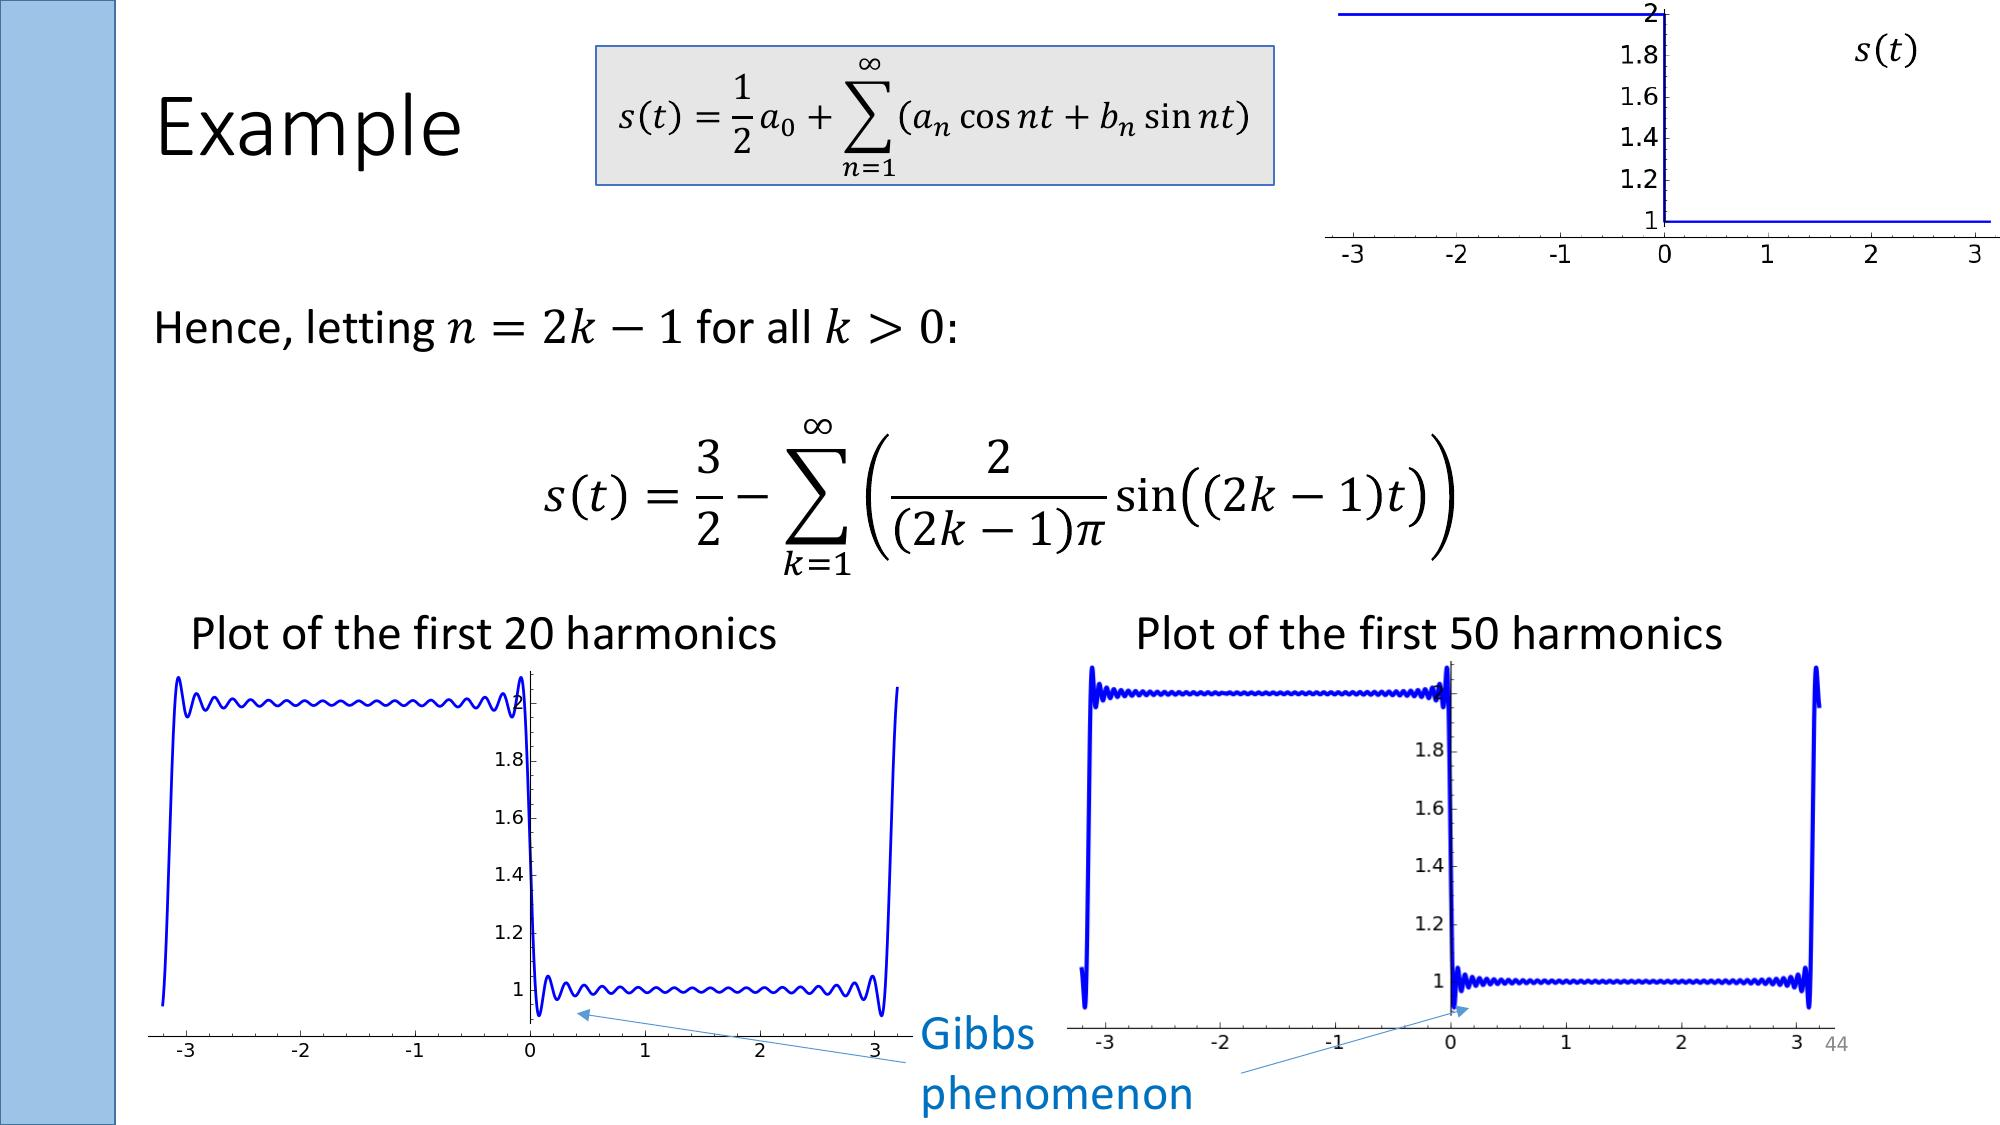
\includegraphics[keepaspectratio]{images/lezione-25-lab-teoria-dei-segnali-introduzione-e-serie-di-fourier-img-05.jpg}}
\caption{Fenomeno di Gibbs: aggiungere più armoniche riduce le
oscillazioni nel tratto piatto, ma l'overshoot al salto rimane costante
(\textasciitilde9\% del salto).}
\end{figure}

\begin{center}\rule{0.5\linewidth}{0.5pt}\end{center}

\section{Serie di Fourier con Periodo
Arbitrario}\label{serie-di-fourier-con-periodo-arbitrario}

La definizione si estende naturalmente a segnali con periodo generico
\(T\). Tramite la sostituzione \(y = 2\pi t / T\), un segnale periodico
in \([-T/2, T/2]\) si trasforma in uno periodico in \([-\pi, \pi]\), e i
coefficienti diventano:

\[s(t) = \frac{1}{2} a_0 + \sum_{n=1}^{\infty} \left( a_n \cos\frac{2\pi n t}{T} + b_n \sin\frac{2\pi n t}{T} \right)\]

con

\[a_0 = \frac{2}{T} \int_{-T/2}^{T/2} s(t)\, dt \qquad a_n = \frac{2}{T} \int_{-T/2}^{T/2} s(t) \cos\frac{2\pi n t}{T}\, dt \qquad b_n = \frac{2}{T} \int_{-T/2}^{T/2} s(t) \sin\frac{2\pi n t}{T}\, dt\]

\begin{center}\rule{0.5\linewidth}{0.5pt}\end{center}

\section{Numeri Complessi e Formula di
Eulero}\label{numeri-complessi-e-formula-di-eulero}

Prima di passare alla forma esponenziale della serie, è necessario
richiamare i \textbf{numeri complessi}. Un numero complesso
\(\bar{x} = a + jb\) ha parte reale \(a\) e parte immaginaria \(b\) (con
\(j = \sqrt{-1}\)). Nel piano complesso è rappresentato come un vettore
di modulo \(|\bar{x}| = \sqrt{a^2 + b^2}\) e fase
\(\varphi = \tan^{-1}(b/a)\).

\begin{calloutdefinition}{Formula di Eulero}

\[e^{\pm j\varphi} = \cos\varphi \pm j\sin\varphi\]

Da cui si derivano le formule inverse:
\[\cos\varphi = \frac{e^{j\varphi} + e^{-j\varphi}}{2} \qquad \sin\varphi = \frac{e^{j\varphi} - e^{-j\varphi}}{2j}\]

\end{calloutdefinition}

Usando l'esponenziale di Eulero, ogni numero complesso si scrive
compattamente come \(\bar{x} = |x| e^{j\varphi}\), che combina modulo e
fase in un unico termine. Questo è particolarmente potente per
rappresentare segnali: ampiezza e fase di ogni armonica vengono
codificate in un unico coefficiente complesso.

\begin{center}\rule{0.5\linewidth}{0.5pt}\end{center}

\section{Serie di Fourier in Forma
Esponenziale}\label{serie-di-fourier-in-forma-esponenziale}

\subsection{La Base Esponenziale}\label{la-base-esponenziale}

La serie di Fourier generalizzata al dominio complesso usa come base
l'insieme di funzioni:

\[e^{j2\pi n F t} \quad \forall n \in \mathbb{Z}\]

poiché \(e^{j2\pi n F t} = \cos(2\pi n F t) + j\sin(2\pi n F t)\), ogni
elemento della base è una sinusoide complessa alla frequenza \(nF\).

\begin{calloutdefinition}{Serie di Fourier esponenziale}

Dato un segnale periodico \(s(t) = s(t+T)\) con frequenza fondamentale
\(F = 1/T\):
\[s(t) = \sum_{n=-\infty}^{+\infty} S_n \, e^{j2\pi n F t}\]

dove i coefficienti \(S_n\) (in generale complessi) si calcolano come:
\[S_n = \frac{1}{T} \int_{0}^{T} s(t) \, e^{-j2\pi n F t}\, dt\]

\end{calloutdefinition}

I coefficienti \(S_n\) codificano sia ampiezza che fase di ogni
armonica: \(S_n = |S_n| e^{j\phi_n}\), dove \(|S_n|\) è l'ampiezza e
\(\phi_n = \arg(S_n)\) è la fase dell'armonica \(n\)-esima.

\subsection{Interpretazione
Geometrica}\label{interpretazione-geometrica}

Per \(n = 0\): la componente continua (media del segnale),
\(S_0 = \frac{1}{T}\int_0^T s(t)\, dt\).\\
Per \(n = \pm 1\): frequenza fondamentale \(F\), periodo \(T\).\\
Per \(|n| > 1\): armoniche di frequenza \(nF\), periodo \(T/n\).

\begin{callouttip}{Perché la forma complessa?}

Con i numeri reali occorrono due coefficienti (\(a_n\) e \(b_n\)) per
descrivere ogni armonica. Con la forma complessa basta un solo
coefficiente \(S_n\) che ne racchiude entrambi. Questo semplifica
enormemente la manipolazione matematica e consente di rappresentare
segnali \(s(t): \mathbb{R} \to \mathbb{C}\), generalizzando la serie per
funzioni reali.

\end{callouttip}

\subsection{Esempio: Onda Rettangolare con Base
Esponenziale}\label{esempio-onda-rettangolare-con-base-esponenziale}

Consideriamo il segnale di periodo \(T\) e frequenza \(F = 1/T\):

\[s(t) = \begin{cases} 1 & \text{se } |t| \le T/4 \\ 0 & \text{se } T/4 < |t| \le T/2 \end{cases}\]

Il calcolo dei coefficienti dà:

\[S_n = \begin{cases} 1/2 & n = 0 \\ 0 & n \text{ pari} \\ \dfrac{(-1)^k}{-(2k-1)\pi} & n = 2k-1 \end{cases}\]

La serie risultante è quindi:

\[s(t) = \frac{1}{2} + \sum_{k=-\infty}^{+\infty} -\frac{(-1)^k}{(2k-1)\pi} \cos\bigl(2\pi(2k-1)Ft\bigr)\]

Il grafico seguente mostra la convergenza della serie per \(T=4\) con
\(k \in [-1,1]\) (verde), \(k \in [-2,2]\) (rosso) e
\(k \in [-100,100]\) (blu):

\begin{figure}
\centering
\pandocbounded{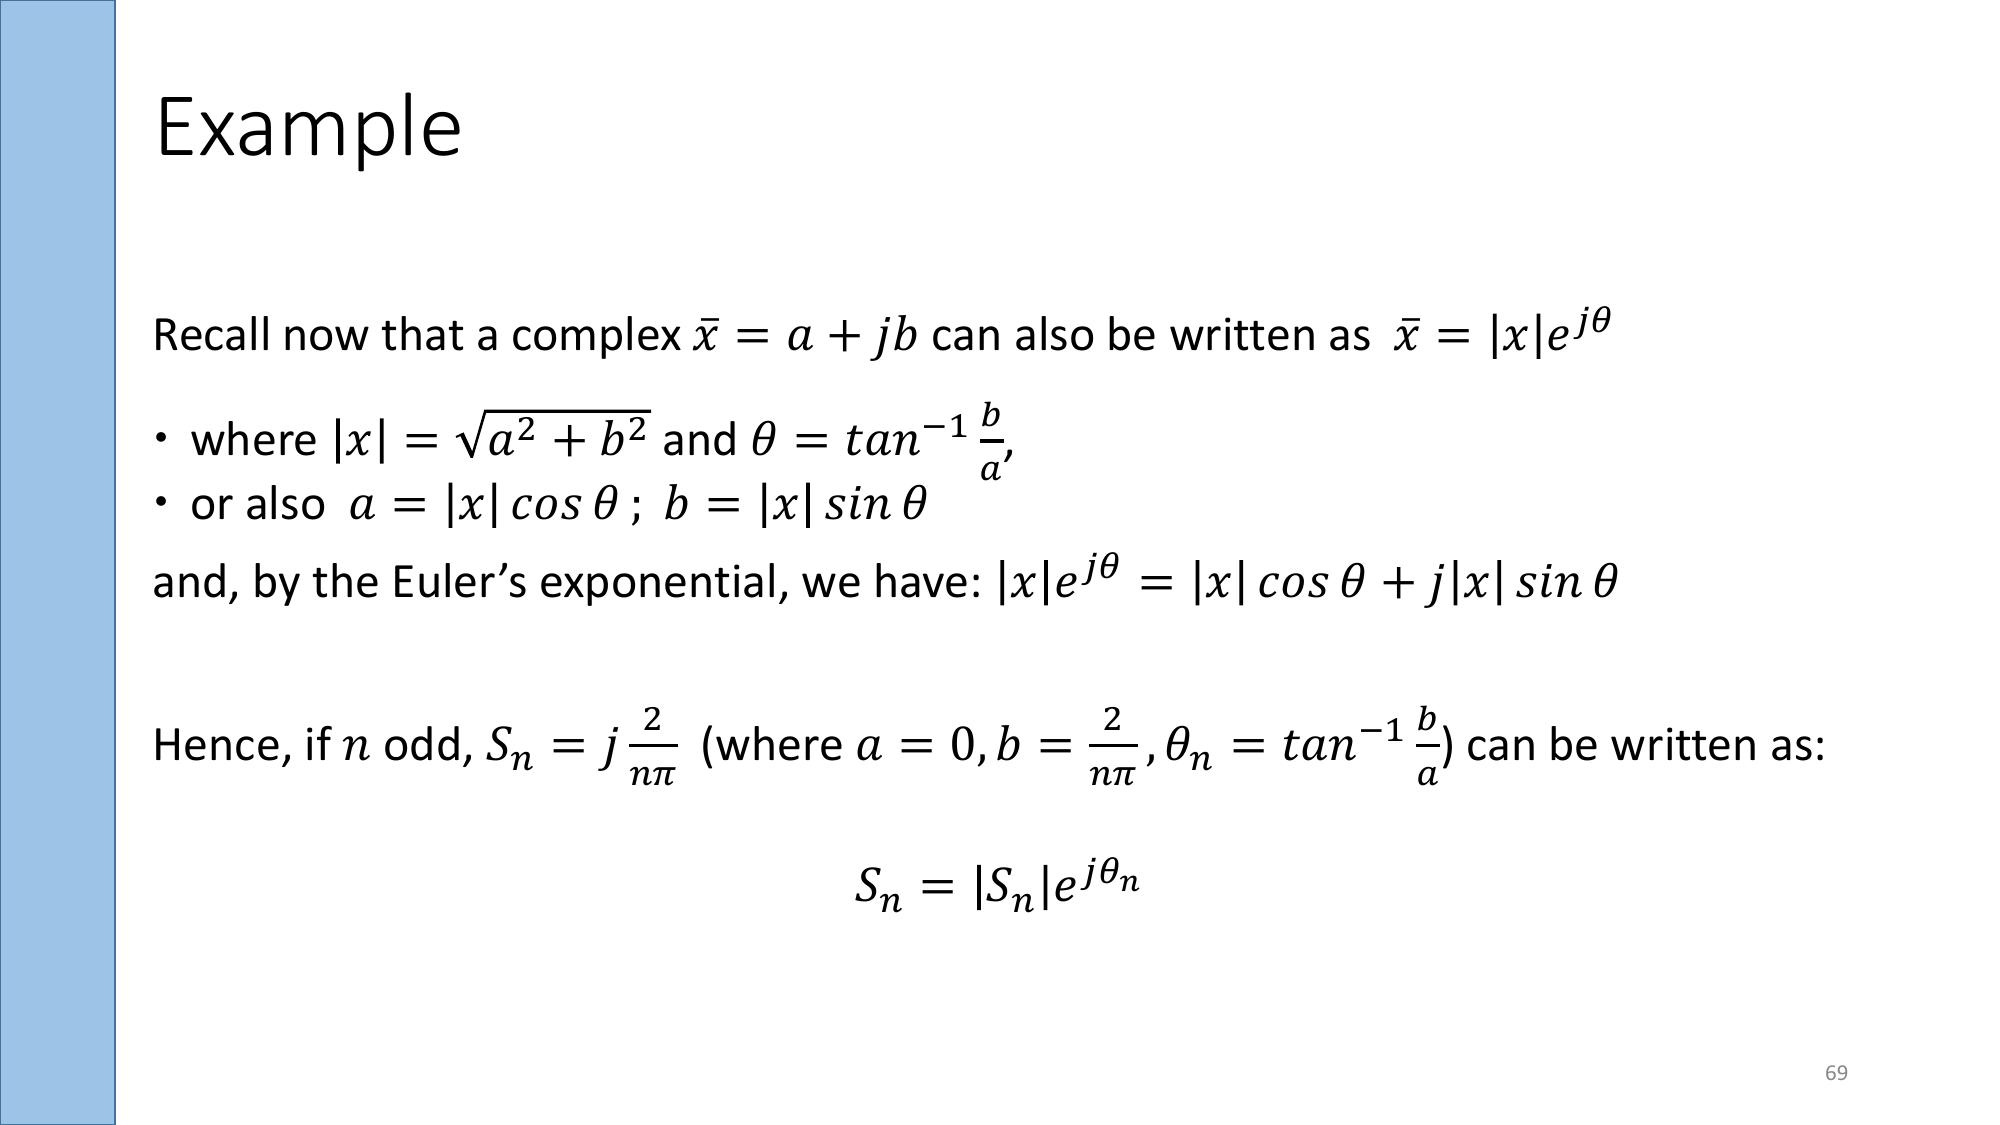
\includegraphics[keepaspectratio]{images/lezione-25-lab-teoria-dei-segnali-introduzione-e-serie-di-fourier-img-06.jpg}}
\caption{Al crescere del numero di armoniche considerate (verde → rosso
→ blu) la serie converge all'onda rettangolare. La forma in blu con
k=100 è quasi perfetta, con il solo fenomeno di Gibbs ai salti.}
\end{figure}

\begin{center}\rule{0.5\linewidth}{0.5pt}\end{center}

\section{Lo Spettro di un Segnale}\label{lo-spettro-di-un-segnale}

La sequenza ordinata dei coefficienti \(\{S_n\}_{n=-\infty}^{+\infty}\)
è chiamata \textbf{spettro} del segnale. Conoscere lo spettro equivale a
conoscere il segnale (dove \(s(t)\) è continua; nei punti di
discontinuità vale la media dei limiti laterali, per il teorema di
Dirichlet).

Poiché i coefficienti \(S_n\) sono in generale numeri complessi anche
quando \(s(t)\) è reale, lo spettro non può essere rappresentato con un
singolo grafico 2D. Si usano invece due diagrammi separati, sfruttando
la rappresentazione \(S_n = |S_n| e^{j\theta_n}\):

\begin{itemize}
\tightlist
\item
  \textbf{Spettro di ampiezza}: il grafico di \(|S_n|\) in funzione di
  \(n\) (o della frequenza \(nF\))
\item
  \textbf{Spettro di fase}: il grafico di \(\theta_n = \arg(S_n)\) in
  funzione di \(n\)
\end{itemize}

\begin{callouttip}{Spettro dell’onda quadra antisimmetrica}

Per il segnale \(s(t) = -1\) se \(0 < t \le T/2\), \(s(t) = 1\) se
\(T/2 < t \le T\), i coefficienti sono:
\[S_n = \begin{cases} 0 & n \text{ pari} \\ \dfrac{2}{n\pi} e^{j\pi/2} & n > 0, \text{ dispari} \\ -\dfrac{2}{n\pi} e^{-j\pi/2} & n < 0, \text{ dispari} \end{cases}\]
Lo spettro di ampiezza decade come \(2/(|n|\pi)\) per gli indici
dispari; lo spettro di fase è costante a \(+\pi/2\) per \(n > 0\) e
\(-\pi/2\) per \(n < 0\).

\end{callouttip}

\begin{center}\rule{0.5\linewidth}{0.5pt}\end{center}

\section{Segnali Aperiodici e Supporto
Limitato}\label{segnali-aperiodici-e-supporto-limitato}

Anche per i segnali aperiodici con supporto limitato a \([a, b)\) ---
cioè \(s(t) = 0\) per \(t \notin [a,b)\) --- è possibile calcolare la
serie di Fourier. Tuttavia, la serie assume implicitamente che il
segnale sia periodico con periodo \(T = b - a\). La conseguenza è che,
invertendo la serie (da \(S_n\) a \(s(t)\)), si ottiene
l'\textbf{estensione periodica} del segnale originale, non il segnale
aperiodico stesso.

\[s^*(t) = \sum_{n=-\infty}^{+\infty} s(t - nT)\]

Questo passaggio è cruciale: la serie di Fourier non può rappresentare
segnali davvero aperiodici. Per questi occorre la \textbf{Trasformata di
Fourier} (argomento delle lezioni successive), che è in un certo senso
il limite della serie di Fourier per \(T \to \infty\).

\begin{center}\rule{0.5\linewidth}{0.5pt}\end{center}

\newpage

\chapter{Lezione 26 --- (Lab) Network
Slicing}\label{lezione-26-lab-network-slicing}

\section{(Lab) Network Slicing con SDN e
ComNetsEmu}\label{lab-network-slicing-con-sdn-e-comnetsemu}

Questa lezione hands-on mette in pratica il concetto di \textbf{network
slicing} partendo dalla teoria del 5G per arrivare a un'implementazione
funzionante basata su {[}{[}Lezione 15 - (Lab) SDN
Architecture\textbar SDN{]}{]} con il controller Ryu e l'emulatore
ComNetsEmu. L'obiettivo centrale è dimostrare come sia possibile
partizionare una singola infrastruttura fisica in sotto-reti logicamente
isolate, ciascuna con garanzie proprie di banda e connettività.

\begin{center}\rule{0.5\linewidth}{0.5pt}\end{center}

\subsection{Contesto: il 5G e la necessità del Network
Slicing}\label{contesto-il-5g-e-la-necessituxe0-del-network-slicing}

Il 5G non è semplicemente un incremento di velocità rispetto al 4G: è
una riprogettazione fondamentale dell'architettura di rete, motivata
dalla coesistenza di tre categorie di servizio con requisiti
radicalmente diversi tra loro.

\begin{calloutdefinition}{mMTC — massive Machine Type Communications}

Comunicazione tra un numero elevatissimo di dispositivi (fino a
200.000/km²), tipicamente sensori a bassa potenza e costo. I requisiti
dominanti sono la \textbf{massima efficienza energetica} e la
\textbf{scalabilità della connessione}, non la latenza o la banda.

\end{calloutdefinition}

\begin{calloutdefinition}{URLLC — Ultra-Reliable Low-Latency Communications}

Servizi che richiedono simultaneamente \textbf{bassa latenza} (≤ 5 ms
per sistemi di trasporto intelligenti, ≤ 1 ms per motion control
industriale) e \textbf{alta affidabilità}. Esempi: guida autonoma, robot
industriali, smart grid.

\end{calloutdefinition}

\begin{calloutdefinition}{eMBB — Enhanced Mobile Broadband}

Servizi ad alta densità di dati: streaming 4K/8K, realtà aumentata e
virtuale, ologrammi. Il requisito primario è la \textbf{capacità di
trasmissione} e la copertura ampia.

\end{calloutdefinition}

La coesistenza di questi tre profili rende impossibile ottimizzare
un'unica rete per tutti contemporaneamente. La soluzione è il
\textbf{network slicing}: invece di una rete monolitica con compromessi
su tutto, si creano più reti virtuali end-to-end sopra la stessa
infrastruttura fisica, ognuna ottimizzata per il proprio caso d'uso.

\begin{center}\rule{0.5\linewidth}{0.5pt}\end{center}

\subsection{Network Slicing: il
concetto}\label{network-slicing-il-concetto}

Il network slicing sfrutta le risorse dell'infrastruttura fisica per
creare multiple \textbf{sotto-reti virtuali} (slice), ciascuna delle
quali si comporta come una rete indipendente dal punto di vista delle
applicazioni che vi girano sopra.

Ogni slice è definita in termini di: - \textbf{funzionalità} --- quali
funzioni di rete sono presenti - \textbf{QoS} --- banda garantita,
latenza massima, tasso di perdita tollerato - \textbf{isolamento} --- le
slice non interferiscono tra loro né in termini di prestazioni né di
sicurezza

\subsubsection{Ruolo di NFV e SDN}\label{ruolo-di-nfv-e-sdn}

Le due tecnologie abilitanti del network slicing sono {[}{[}Lezione 20 -
(Lab) Network Function Virtualization\textbar NFV{]}{]} e {[}{[}Lezione
15 - (Lab) SDN Architecture\textbar SDN{]}{]}, con ruoli complementari.

\textbf{NFV} (Network Function Virtualization) si occupa di
\emph{implementare} le funzioni di rete di ogni slice come Virtual
Network Functions (VNF) eseguite su hardware commodity. L'isolamento tra
slice è garantito dalla virtualizzazione: ogni VNF vede solo le risorse
assegnatele, indipendentemente dalle altre slice sulla stessa macchina
fisica.

\textbf{SDN} (Software-Defined Networking) si occupa di \emph{governare}
il comportamento del traffico all'interno di ogni slice. Una volta
definita la slice, il controller SDN monitora e impone i requisiti di
QoS installando le flow rule appropriate sugli switch.

\subsubsection{Architettura generica per il Network
Slicing}\label{architettura-generica-per-il-network-slicing}

\begin{figure}
\centering
\pandocbounded{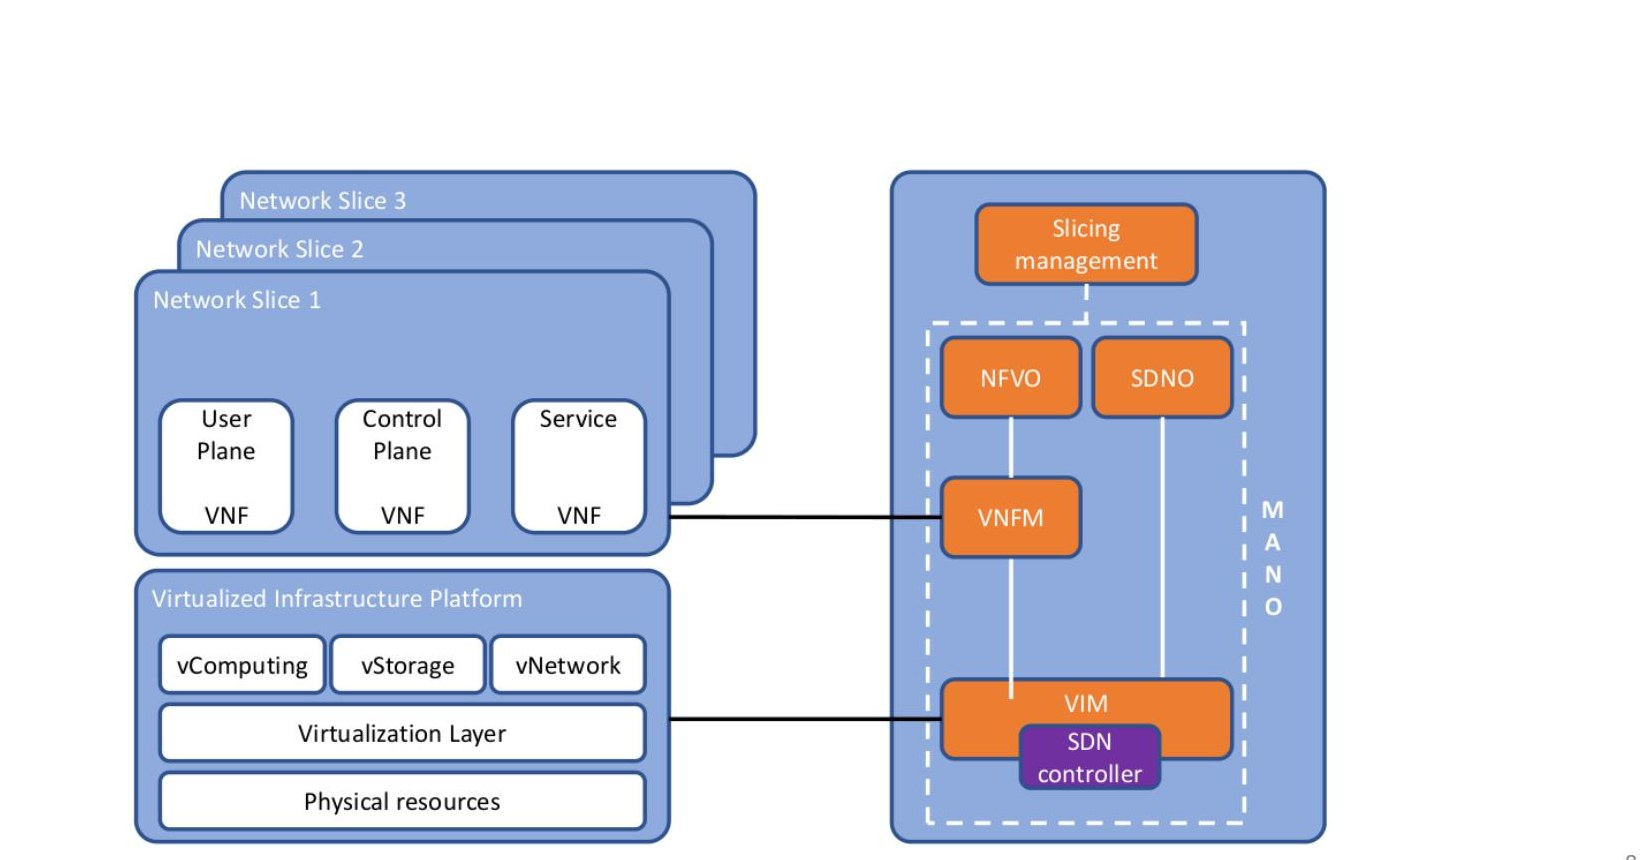
\includegraphics[keepaspectratio,alt={Architettura generica per il network slicing}]{images/lezione-26-lab-network-slicing-img-01.jpg}}
\caption{Architettura generica per il network slicing}
\end{figure}

\emph{Fig. --- Architettura generica per il network slicing: le slice
(sinistra) poggiano sull'infrastruttura virtualizzata, gestita dal
framework MANO (destra).}

Il piano di gestione (MANO) si articola su più livelli:

\begin{itemize}
\tightlist
\item
  \textbf{Slicing Management}: punto di ingresso per la definizione
  delle slice
\item
  \textbf{NFVO} (NFV Orchestrator): orchestra le risorse NFV a livello
  di sistema
\item
  \textbf{SDNO} (SDN Orchestrator): orchestra le risorse SDN
\item
  \textbf{VNFM} (VNF Manager): gestisce il ciclo di vita di ogni singola
  VNF (creazione, scaling, terminazione)
\item
  \textbf{VIM} (Virtualized Infrastructure Manager): controlla
  direttamente le risorse virtualizzate (compute, storage, network)
\item
  \textbf{SDN Controller}: implementa la logica di forwarding sugli
  switch
\end{itemize}

\subsubsection{Il caso d'uso 5G con RAN}\label{il-caso-duso-5g-con-ran}

In un deployment 5G reale, l'architettura a slice percorre tutta la rete
dall'accesso radio al core cloud. La \textbf{Radio Access Network (RAN)}
è scomposta in tre unità funzionali:

\begin{itemize}
\tightlist
\item
  \textbf{Radio Unit (RU)}: l'hardware radio fisico, tipicamente
  sull'antenna
\item
  \textbf{Distributed Unit (DU)}: elabora i livelli MAC e Fisico,
  distribuita vicino alla RU
\item
  \textbf{Centralized Unit (CU)}: gestisce i protocolli di livello
  superiore (RRC, PDCP) e può essere ospitata nel cloud
\end{itemize}

Slice diverse (UHD, Phone, Massive IoT, Mission-critical IoT)
attraversano la stessa RAN ma mantengono path di dati separati sia
nell'Edge Cloud (NFV) sia nel Core Cloud (NFV), con controller SDN
dedicati a ogni livello.

\begin{center}\rule{0.5\linewidth}{0.5pt}\end{center}

\subsection{Topologia dell'esperimento}\label{topologia-dellesperimento}

L'esperimento implementa il network slicing su scala ridotta usando
\textbf{ComNetsEmu} come emulatore e \textbf{Ryu} come controller SDN.
La rete è organizzata come segue.

\subsubsection{Descrizione della rete
fisica}\label{descrizione-della-rete-fisica}

\begin{figure}
\centering
\pandocbounded{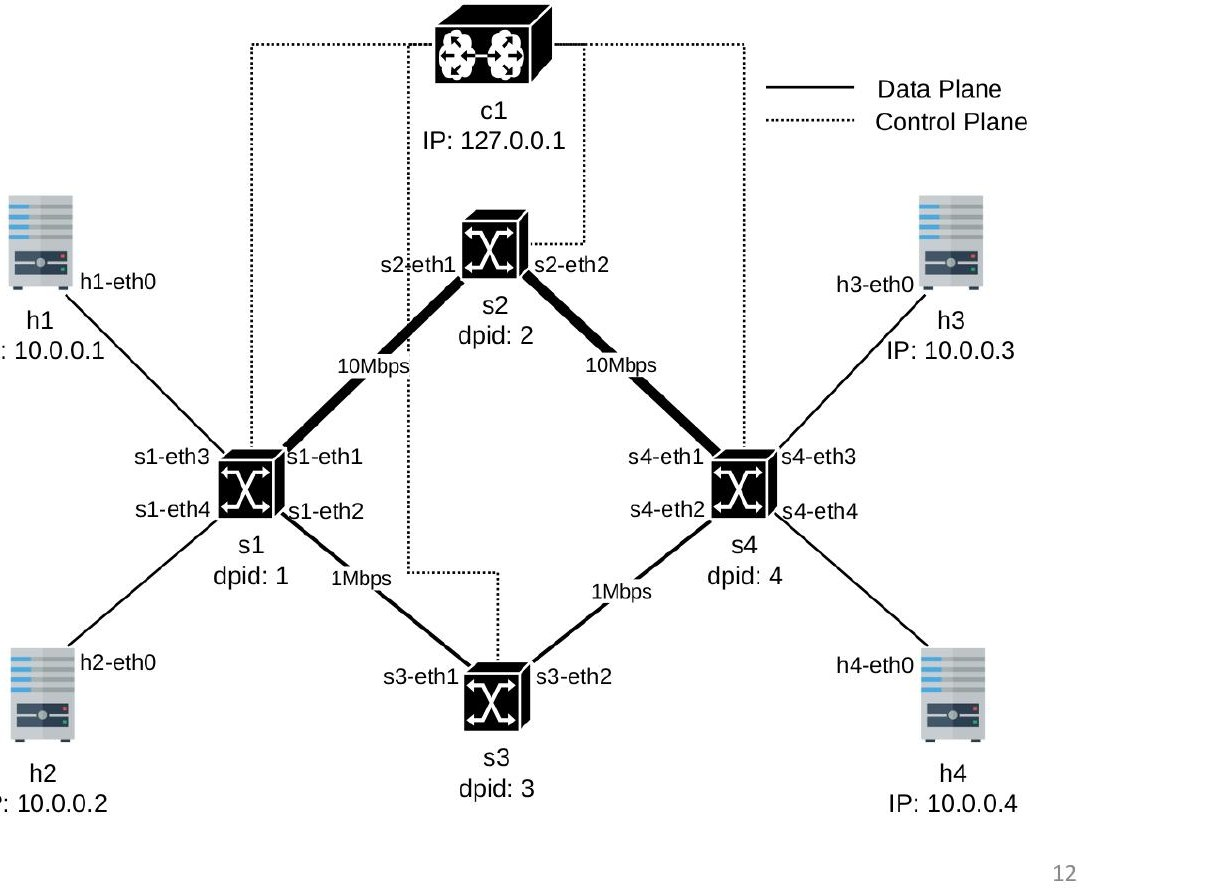
\includegraphics[keepaspectratio,alt={Topologia ad anello con quattro switch e quattro host}]{images/lezione-26-lab-network-slicing-img-02.jpg}}
\caption{Topologia ad anello con quattro switch e quattro host}
\end{figure}

\emph{Fig. --- Topologia ad anello: il percorso superiore (S1→S2→S4) a
10 Mbps è destinato alla slice video; quello inferiore (S1→S3→S4) a 1
Mbps alla slice HTTP. Le linee tratteggiate rappresentano il control
plane.}

La topologia è un \textbf{anello di quattro switch} (S1, S2, S3, S4) con
host alle estremità:

\begin{itemize}
\tightlist
\item
  S1 ha quattro porte: eth1 verso S2, eth2 verso S3, eth3 verso h1, eth4
  verso h2
\item
  S4 ha la stessa struttura speculare: eth1 verso S2, eth2 verso S3,
  eth3 verso h3, eth4 verso h4
\item
  S2 e S3 sono semplicemente di transito: due porte, una verso S1 e una
  verso S4
\item
  I link superiori (via S2) hanno banda 10 Mbps; quelli inferiori (via
  S3) hanno banda 1 Mbps
\end{itemize}

\subsubsection{Obiettivo: il Topology
Slicing}\label{obiettivo-il-topology-slicing}

L'obiettivo non è realizzare un instradamento tradizionale (dove tutti
gli host si raggiungono), ma imporre un \textbf{partizionamento rigido}
della topologia:

\begin{itemize}
\tightlist
\item
  \textbf{Upper Slice}: h1 ↔ h3, interconnessi esclusivamente tramite i
  link a 10 Mbps (via S2)
\item
  \textbf{Lower Slice}: h2 ↔ h4, interconnessi esclusivamente tramite i
  link a 1 Mbps (via S3)
\end{itemize}

\begin{calloutwarning}{Isolamento completo}

h1 e h2 non possono comunicare tra loro, anche se sono entrambi
collegati a S1. Il controller impone che il traffico entrante da eth3
(h1) esca solo da eth1 (verso S2), e il traffico da eth4 (h2) esca solo
da eth2 (verso S3). La separazione è logica, non fisica.

\end{calloutwarning}

\begin{figure}
\centering
\pandocbounded{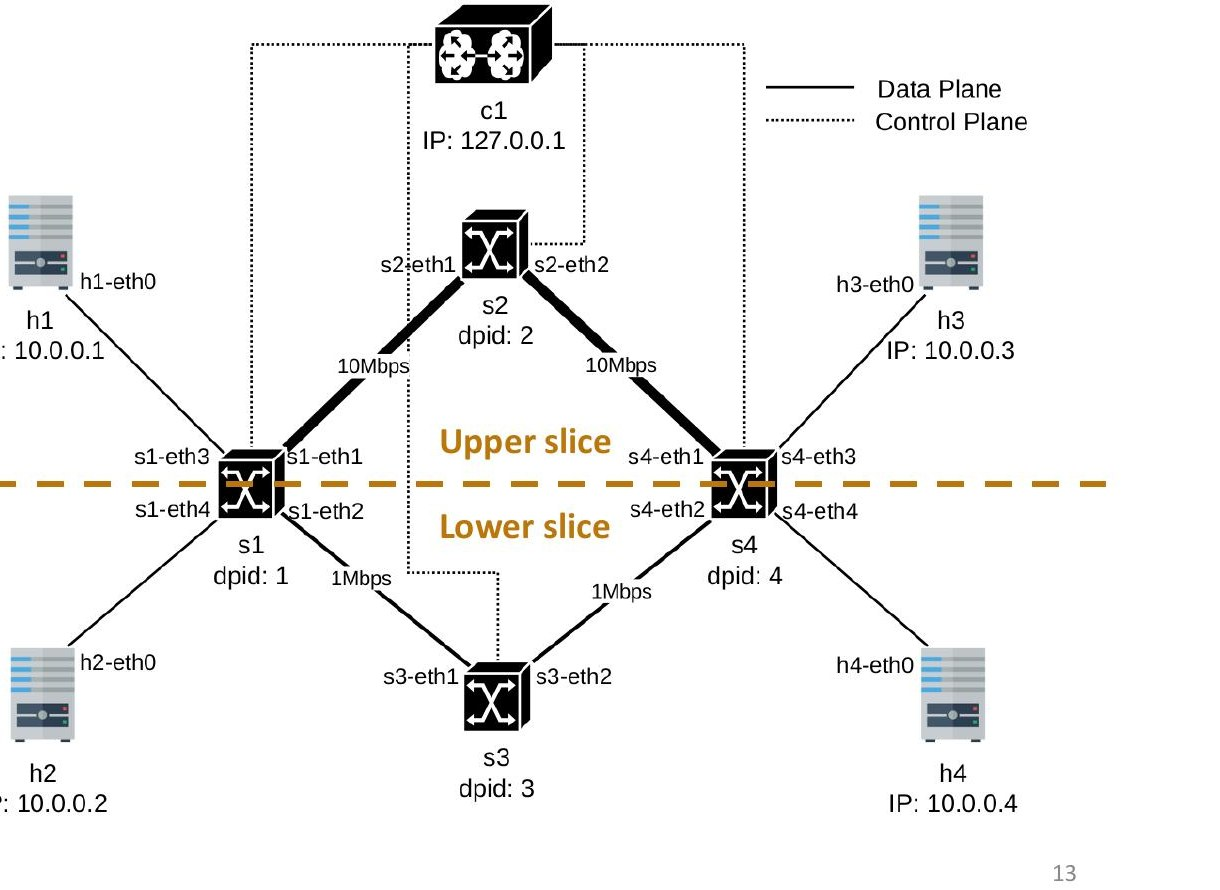
\includegraphics[keepaspectratio]{images/lezione-26-lab-network-slicing-img-03.jpg}}
\caption{Le due slice risultanti: la linea arancione separa l'Upper
Slice (S1-eth1/eth3 ↔ S2 ↔ S4-eth1/eth3) dalla Lower Slice (S1-eth2/eth4
↔ S3 ↔ S4-eth2/eth4).}
\end{figure}

Ogni host ha quindi una propria \textbf{vista della rete}: dal punto di
vista di h1, la rete è semplicemente un collegamento diretto verso h3 a
10 Mbps; h2 e h4 sono invisibili.

\begin{center}\rule{0.5\linewidth}{0.5pt}\end{center}

\subsection{Implementazione con Ryu e
Mininet}\label{implementazione-con-ryu-e-mininet}

Il laboratorio si basa su due script Python nella directory
\texttt{comnetsemu/app/realizing\_network\_slicing/}:

\begin{enumerate}
\def\labelenumi{\arabic{enumi}.}
\tightlist
\item
  \texttt{network.py} --- definisce la topologia e avvia Mininet
\item
  \texttt{topologyslicing.py} --- applicazione Ryu che programma il
  comportamento degli switch
\end{enumerate}

\subsubsection{network.py: definizione della
topologia}\label{network.py-definizione-della-topologia}

Lo script costruisce la topologia usando le API di Mininet. I punti
chiave sono la configurazione dei link con limitazione di banda
(\texttt{TCLink}) e l'assegnazione di DPID univoci agli switch.

\begin{Shaded}
\begin{Highlighting}[]
\NormalTok{host\_config }\OperatorTok{=} \BuiltInTok{dict}\NormalTok{(inNamespace}\OperatorTok{=}\VariableTok{True}\NormalTok{)}
\NormalTok{http\_link\_config }\OperatorTok{=} \BuiltInTok{dict}\NormalTok{(bw}\OperatorTok{=}\DecValTok{1}\NormalTok{)   }\CommentTok{\# 1 Mbps}
\NormalTok{video\_link\_config }\OperatorTok{=} \BuiltInTok{dict}\NormalTok{(bw}\OperatorTok{=}\DecValTok{10}\NormalTok{) }\CommentTok{\# 10 Mbps}

\CommentTok{\#\# Switch con DPID esplicito}
\ControlFlowTok{for}\NormalTok{ i }\KeywordTok{in} \BuiltInTok{range}\NormalTok{(}\DecValTok{4}\NormalTok{):}
\NormalTok{    sconfig }\OperatorTok{=}\NormalTok{ \{}\StringTok{"dpid"}\NormalTok{: }\StringTok{"}\SpecialCharTok{\%016x}\StringTok{"} \OperatorTok{\%}\NormalTok{ (i }\OperatorTok{+} \DecValTok{1}\NormalTok{)\}}
    \VariableTok{self}\NormalTok{.addSwitch(}\StringTok{"s}\SpecialCharTok{\%d}\StringTok{"} \OperatorTok{\%}\NormalTok{ (i }\OperatorTok{+} \DecValTok{1}\NormalTok{), }\OperatorTok{**}\NormalTok{sconfig)}

\CommentTok{\#\# Link tra switch: ordine importante per i numeri di porta!}
\VariableTok{self}\NormalTok{.addLink(}\StringTok{"s1"}\NormalTok{, }\StringTok{"s2"}\NormalTok{, }\OperatorTok{**}\NormalTok{video\_link\_config)  }\CommentTok{\# s1{-}eth1 ↔ s2{-}eth1}
\VariableTok{self}\NormalTok{.addLink(}\StringTok{"s2"}\NormalTok{, }\StringTok{"s4"}\NormalTok{, }\OperatorTok{**}\NormalTok{video\_link\_config)  }\CommentTok{\# s2{-}eth2 ↔ s4{-}eth1}
\VariableTok{self}\NormalTok{.addLink(}\StringTok{"s1"}\NormalTok{, }\StringTok{"s3"}\NormalTok{, }\OperatorTok{**}\NormalTok{http\_link\_config)   }\CommentTok{\# s1{-}eth2 ↔ s3{-}eth1}
\VariableTok{self}\NormalTok{.addLink(}\StringTok{"s3"}\NormalTok{, }\StringTok{"s4"}\NormalTok{, }\OperatorTok{**}\NormalTok{http\_link\_config)   }\CommentTok{\# s3{-}eth2 ↔ s4{-}eth2}

\CommentTok{\#\# Host: h1,h2 su s1; h3,h4 su s4}
\VariableTok{self}\NormalTok{.addLink(}\StringTok{"h1"}\NormalTok{, }\StringTok{"s1"}\NormalTok{)  }\CommentTok{\# → s1{-}eth3}
\VariableTok{self}\NormalTok{.addLink(}\StringTok{"h2"}\NormalTok{, }\StringTok{"s1"}\NormalTok{)  }\CommentTok{\# → s1{-}eth4}
\VariableTok{self}\NormalTok{.addLink(}\StringTok{"h3"}\NormalTok{, }\StringTok{"s4"}\NormalTok{)  }\CommentTok{\# → s4{-}eth3}
\VariableTok{self}\NormalTok{.addLink(}\StringTok{"h4"}\NormalTok{, }\StringTok{"s4"}\NormalTok{)  }\CommentTok{\# → s4{-}eth4}
\end{Highlighting}
\end{Shaded}

\begin{callouttip}{Ordine dei link = numeri di porta}

In Mininet, le porte di uno switch vengono numerate nell'ordine in cui i
link vengono aggiunti. Poiché S1 ottiene prima il link verso S2 (eth1),
poi verso S3 (eth2), poi h1 (eth3) e h4 (eth4), le porte hanno
esattamente questi numeri. Lo stesso vale per S4. Questo dettaglio è
fondamentale per capire la tabella \texttt{slice\_to\_port} in
\texttt{topologyslicing.py}.

\end{callouttip}

La rete viene avviata con un \textbf{controller remoto} (Ryu) in ascolto
su \texttt{127.0.0.1:6633}, e \texttt{autoStaticArp=True} per evitare
che i pacchetti ARP broadcast debbano essere gestiti dalla logica di
slicing.

\subsubsection{Programmare una rete SDN con
Ryu}\label{programmare-una-rete-sdn-con-ryu}

\textbf{Ryu} è un framework per controller SDN scritto in Python. Si
basa su un modello a \textbf{eventi}: l'applicazione si registra per
ricevere notifiche di specifici eventi di rete (arrivo di un pacchetto,
connessione/disconnessione di uno switch, cambio di link) e reagisce
installando o modificando le flow rule.

\begin{figure}
\centering
\pandocbounded{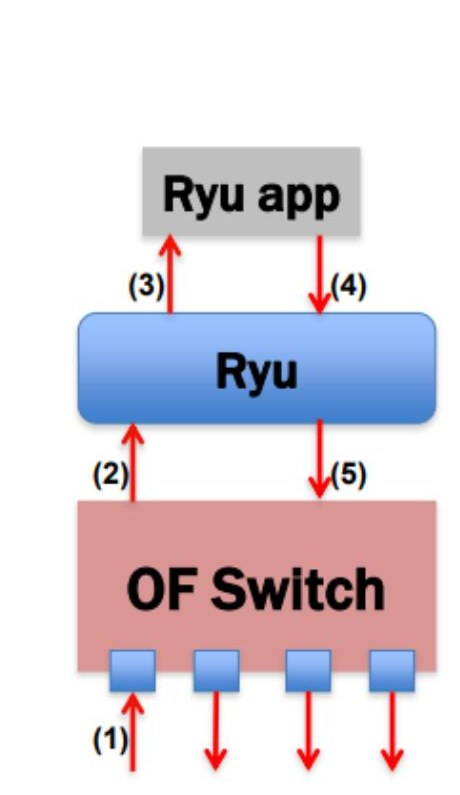
\includegraphics[keepaspectratio,alt={Architettura Ryu: Ryu app sopra il layer Ryu sopra l'OF Switch}]{images/lezione-26-lab-network-slicing-img-04.jpg}}
\caption{Architettura Ryu: Ryu app sopra il layer Ryu sopra l'OF Switch}
\end{figure}

\emph{Fig. --- Stack Ryu: la Ryu app riceve eventi (frecce ③) e invia
comandi (frecce ④) al layer Ryu, che comunica con l'OF Switch tramite
OpenFlow (frecce ②⑤).}

Una \textbf{Ryu app} è una classe Python che: 1. Estende
\texttt{ryu.base.app\_manager.RyuApp} 2. Dichiara la versione di
OpenFlow supportata (\texttt{OFP\_VERSIONS}) 3. Registra handler per
specifici eventi con il decoratore \texttt{@set\_ev\_cls}

\subsubsection{topologyslicing.py: la logica del
controller}\label{topologyslicing.py-la-logica-del-controller}

\paragraph{Inizializzazione e
slice\_to\_port}\label{inizializzazione-e-slice_to_port}

Il cuore della logica di slicing è il dizionario
\texttt{slice\_to\_port}, che mappa per ogni switch (identificato dal
DPID) quale porta di uscita usare a seconda della porta di ingresso:

\begin{Shaded}
\begin{Highlighting}[]
\VariableTok{self}\NormalTok{.slice\_to\_port }\OperatorTok{=}\NormalTok{ \{}
    \DecValTok{1}\NormalTok{: \{}\DecValTok{1}\NormalTok{: }\DecValTok{3}\NormalTok{, }\DecValTok{3}\NormalTok{: }\DecValTok{1}\NormalTok{, }\DecValTok{2}\NormalTok{: }\DecValTok{4}\NormalTok{, }\DecValTok{4}\NormalTok{: }\DecValTok{2}\NormalTok{\},  }\CommentTok{\# S1: eth1↔eth3 (upper), eth2↔eth4 (lower)}
    \DecValTok{4}\NormalTok{: \{}\DecValTok{1}\NormalTok{: }\DecValTok{3}\NormalTok{, }\DecValTok{3}\NormalTok{: }\DecValTok{1}\NormalTok{, }\DecValTok{2}\NormalTok{: }\DecValTok{4}\NormalTok{, }\DecValTok{4}\NormalTok{: }\DecValTok{2}\NormalTok{\},  }\CommentTok{\# S4: stesso schema di S1}
    \DecValTok{2}\NormalTok{: \{}\DecValTok{1}\NormalTok{: }\DecValTok{2}\NormalTok{, }\DecValTok{2}\NormalTok{: }\DecValTok{1}\NormalTok{\},               }\CommentTok{\# S2: forwarding diretto}
    \DecValTok{3}\NormalTok{: \{}\DecValTok{1}\NormalTok{: }\DecValTok{2}\NormalTok{, }\DecValTok{2}\NormalTok{: }\DecValTok{1}\NormalTok{\},               }\CommentTok{\# S3: forwarding diretto}
\NormalTok{\}}
\end{Highlighting}
\end{Shaded}

\begin{callouttip}{Lettura della tabella per S1}

Per S1 (dpid=1): se un pacchetto arriva su eth1 (da S2, upper path),
viene inoltrato su eth3 (verso h1). Se arriva su eth3 (da h1), torna su
eth1 (verso S2). Specularmente, eth2 (da S3, lower path) ↔ eth4 (verso
h2). Il traffico di h1 non può mai raggiungere eth2 o eth4, garantendo
l'isolamento.

\end{callouttip}

La separazione è quindi \textbf{esclusivamente statistica su S1 e S4}:
S2 e S3 non devono fare nulla di speciale, perché non ricevono mai
traffico cross-slice (la separazione avviene prima di loro).

\paragraph{Gestione degli eventi
OpenFlow}\label{gestione-degli-eventi-openflow}

La classe gestisce due eventi principali:

\textbf{\texttt{switch\_features\_handler}} (evento
\texttt{EventOFPSwitchFeatures}, fase \texttt{CONFIG\_DISPATCHER}):
viene invocato quando uno switch si connette al controller per la prima
volta. Installa la \textbf{table-miss flow entry} con priorità 0 e match
vuoto (corrisponde a qualsiasi pacchetto): l'azione è inviare al
controller con \texttt{OFPP\_CONTROLLER}. Questa regola garantisce che i
primi pacchetti di ogni flusso vengano consegnati all'applicazione.

\textbf{\texttt{\_packet\_in\_handler}} (evento
\texttt{EventOFPPacketIn}, fase \texttt{MAIN\_DISPATCHER}): viene
invocato ogni volta che uno switch riceve un pacchetto senza una flow
rule corrispondente e lo manda al controller. La logica è:

\begin{enumerate}
\def\labelenumi{\arabic{enumi}.}
\tightlist
\item
  Legge il DPID dello switch e la porta di ingresso
\item
  Consulta \texttt{slice\_to\_port} per determinare la porta di uscita
\item
  Installa una \textbf{flow rule permanente} con \texttt{add\_flow}
  (così i pacchetti successivi dello stesso flusso non passeranno più
  dal controller)
\item
  Invia immediatamente il pacchetto corrente con
  \texttt{\_send\_package}
\end{enumerate}

\begin{Shaded}
\begin{Highlighting}[]
\KeywordTok{def}\NormalTok{ \_packet\_in\_handler(}\VariableTok{self}\NormalTok{, ev):}
\NormalTok{    msg }\OperatorTok{=}\NormalTok{ ev.msg}
\NormalTok{    datapath }\OperatorTok{=}\NormalTok{ msg.datapath}
\NormalTok{    in\_port }\OperatorTok{=}\NormalTok{ msg.match[}\StringTok{"in\_port"}\NormalTok{]}
\NormalTok{    dpid }\OperatorTok{=}\NormalTok{ datapath.}\BuiltInTok{id}

\NormalTok{    out\_port }\OperatorTok{=} \VariableTok{self}\NormalTok{.slice\_to\_port[dpid][in\_port]}

\NormalTok{    actions }\OperatorTok{=}\NormalTok{ [datapath.ofproto\_parser.OFPActionOutput(out\_port)]}
\NormalTok{    match }\OperatorTok{=}\NormalTok{ datapath.ofproto\_parser.OFPMatch(in\_port}\OperatorTok{=}\NormalTok{in\_port)}
    \VariableTok{self}\NormalTok{.add\_flow(datapath, }\DecValTok{1}\NormalTok{, match, actions)}
    \VariableTok{self}\NormalTok{.\_send\_package(msg, datapath, in\_port, actions)}
\end{Highlighting}
\end{Shaded}

\textbf{\texttt{add\_flow}} costruisce e invia un messaggio
\texttt{OFPFlowMod} al datapath (lo switch), che modifica la flow table
installando la nuova regola. Da quel momento in poi, i pacchetti che
corrispondono al match vengono gestiti direttamente dallo switch senza
coinvolgere il controller.

\begin{calloutnote}{Reactive vs Proactive flow installation}

Questa applicazione usa l'approccio \textbf{reattivo}: le regole vengono
installate al primo pacchetto. In alternativa, un controller
\textbf{proattivo} potrebbe installare tutte le regole all'avvio
(\texttt{switch\_features\_handler}) senza aspettare traffico reale. Per
questo schema di slicing statico, l'approccio proattivo sarebbe più
efficiente poiché elimina la latenza del primo pacchetto.

\end{calloutnote}

\begin{center}\rule{0.5\linewidth}{0.5pt}\end{center}

\subsection{Esercizi}\label{esercizi}

\subsubsection{Esercizio A: esecuzione e
verifica}\label{esercizio-a-esecuzione-e-verifica}

L'avvio richiede due terminali distinti (il controller e Mininet devono
girare in parallelo):

\begin{Shaded}
\begin{Highlighting}[]
\CommentTok{\#\# Terminale 1 — avvia il controller Ryu}
\ExtensionTok{ryu{-}manager}\NormalTok{ topology\_slicing.py}

\CommentTok{\#\# Terminale 2 — avvia Mininet (richiede sudo)}
\FunctionTok{sudo}\NormalTok{ python3 network.py}
\end{Highlighting}
\end{Shaded}

Una volta avviata la rete, si possono eseguire le verifiche:

\textbf{1. Verifica dell'isolamento (ping)}

Il ping deve avere successo solo tra host della stessa slice. Se la
slicing funziona correttamente: - \texttt{h1\ ping\ h3} → successo
(upper slice) - \texttt{h2\ ping\ h4} → successo (lower slice) -
\texttt{h1\ ping\ h2} → fallimento (cross-slice, non esiste path)

\textbf{2. Verifica della banda (iperf)}

\begin{Shaded}
\begin{Highlighting}[]
\CommentTok{\#\# Nel terminale Mininet}
\ExtensionTok{mininet}\OperatorTok{\textgreater{}}\NormalTok{ iperf h1 h3   }\CommentTok{\# deve mostrare \textasciitilde{}10 Mbps}
\ExtensionTok{mininet}\OperatorTok{\textgreater{}}\NormalTok{ iperf h2 h4   }\CommentTok{\# deve mostrare \textasciitilde{}1 Mbps}
\end{Highlighting}
\end{Shaded}

\textbf{3. Ispezione delle flow rule installate}

\begin{Shaded}
\begin{Highlighting}[]
\ExtensionTok{mininet}\OperatorTok{\textgreater{}}\NormalTok{ sh ovs{-}ofctl dump{-}flows s1}
\end{Highlighting}
\end{Shaded}

Dopo il primo ping tra h1 e h3, devono essere visibili due flow entry su
S1: - match \texttt{in\_port=1} → action \texttt{output:3} - match
\texttt{in\_port=3} → action \texttt{output:1}

La regola di default (table-miss, priorità 0) ha action
\texttt{CONTROLLER}, visibile anche prima del ping.

\textbf{4. Cattura e analisi dei messaggi OpenFlow}

Per osservare il ciclo completo di comunicazione controller-switch, si
può catturare il traffico sulla porta 6633 con tcpdump e analizzarlo in
Wireshark:

\begin{Shaded}
\begin{Highlighting}[]
\CommentTok{\#\# Apri un nuovo terminale}
\FunctionTok{sudo}\NormalTok{ tcpdump }\AttributeTok{{-}i}\NormalTok{ any port 6633 }\AttributeTok{{-}w}\NormalTok{ ofcapturedel.pcap}

\CommentTok{\#\# Cancella le flow rule su s1 per forzare nuovi PACKET\_IN}
\ExtensionTok{mininet}\OperatorTok{\textgreater{}}\NormalTok{ sh ovs{-}ofctl del{-}flows s1 table=0,in\_port=}\StringTok{"s1{-}eth1"}
\ExtensionTok{mininet}\OperatorTok{\textgreater{}}\NormalTok{ sh ovs{-}ofctl del{-}flows s1 table=0,in\_port=}\StringTok{"s1{-}eth3"}

\CommentTok{\#\# Genera traffico e osserva i messaggi}
\ExtensionTok{mininet}\OperatorTok{\textgreater{}}\NormalTok{ h1 ping h3}
\end{Highlighting}
\end{Shaded}

In Wireshark si possono distinguere tre tipi di messaggi OpenFlow
rilevanti: - \texttt{PACKET\_IN}: lo switch invia il pacchetto al
controller (manca la flow rule) - \texttt{PACKET\_OUT}: il controller
risponde con l'azione immediata per il pacchetto corrente -
\texttt{FLOW\_MOD}: il controller installa la regola permanente sullo
switch

\newpage

\chapter{Teoria dei Segnali: Trasformata di Fourier, Campionamento e
DFT}\label{teoria-dei-segnali-trasformata-di-fourier-campionamento-e-dft}

Questa lezione è la continuazione diretta della {[}{[}Lezione 25 - (Lab)
Teoria dei Segnali - Introduzione e Serie di Fourier\textbar Lezione
25{]}{]}, che ha introdotto la classificazione dei segnali, la
trasmissione, la serie di Fourier e lo spettro. Qui si affronta il salto
concettuale fondamentale: estendere l'analisi in frequenza ai segnali
\textbf{non periodici} mediante la Trasformata di Fourier, poi si passa
al problema pratico della conversione analogico-digitale e all'analisi
spettrale di segnali campionati tramite la DFT.

\begin{center}\rule{0.5\linewidth}{0.5pt}\end{center}

\section{Trasformata di Fourier}\label{trasformata-di-fourier}

\subsection{Dal Discreto al Continuo: Passaggio dalla Serie alla
Trasformata}\label{dal-discreto-al-continuo-passaggio-dalla-serie-alla-trasformata}

La serie di Fourier, vista nella lezione precedente, funziona bene per
segnali periodici: rappresenta il segnale come somma di armoniche a
frequenze discrete \(nF = n/T\). Ma la stragrande maggioranza dei
segnali reali di interesse --- impulsi, transitori, frammenti audio,
burst radio --- non sono periodici. Come estendere l'analisi in
frequenza a questi segnali?

L'idea è elegante: si considera il segnale non periodico come il limite
di un segnale periodico il cui periodo \(T\) tende all'infinito. Quando
\(T\) cresce, la frequenza fondamentale \(F = 1/T\) diminuisce, e le
armoniche discrete \(nF\) si avvicinano sempre di più tra loro. Nel
limite \(T \to \infty\), la spaziatura tra le armoniche
\(\Delta_f = 1/T \to 0\) e lo spettro discreto diventa uno
\textbf{spettro continuo}.

\begin{figure}
\centering
\pandocbounded{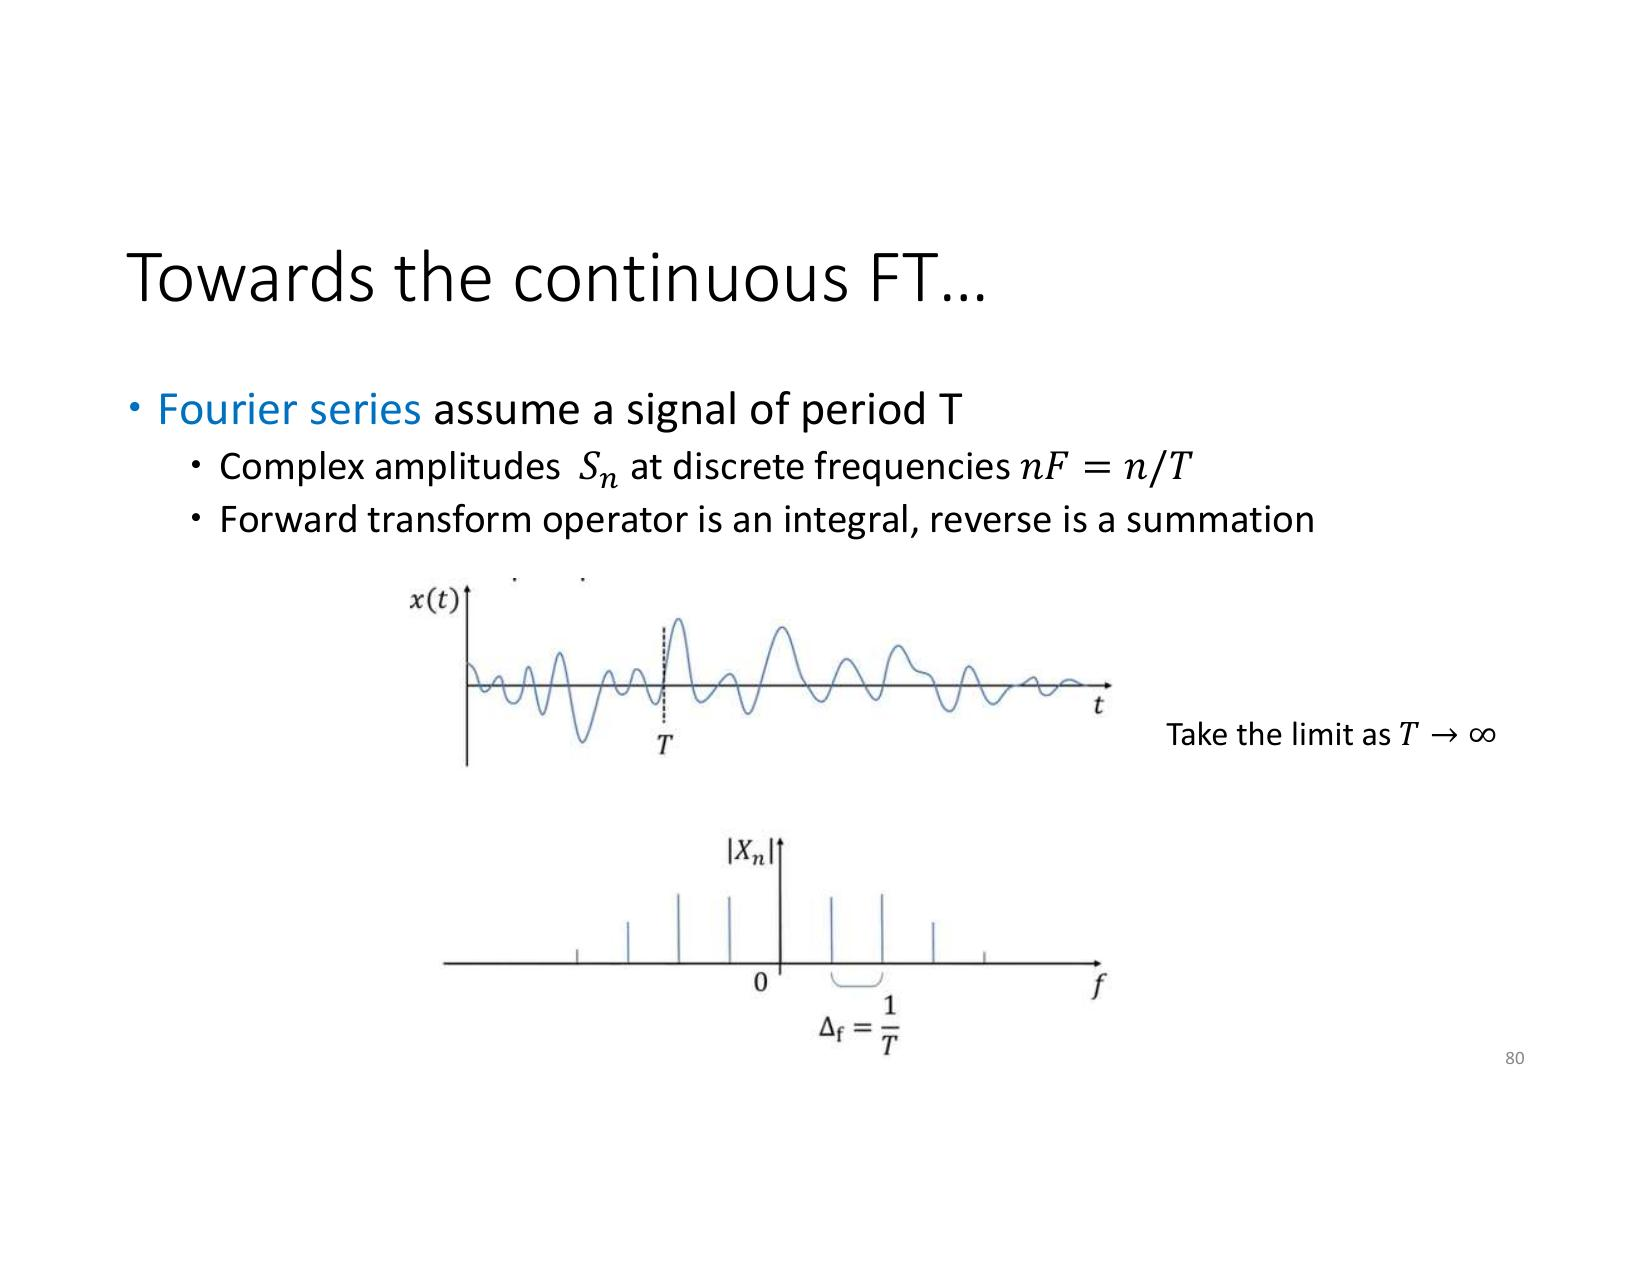
\includegraphics[keepaspectratio]{images/lezione-27-lab-teoria-dei-segnali-trasformata-di-fourier-campionamento-e-dft-img-01.jpg}}
\caption{Segnale periodico e relativo spettro discreto. All'aumentare di
T, le righe spettrali si avvicinano. Prendendo il limite T→∞ si ottiene
lo spettro continuo.}
\end{figure}

\begin{figure}
\centering
\pandocbounded{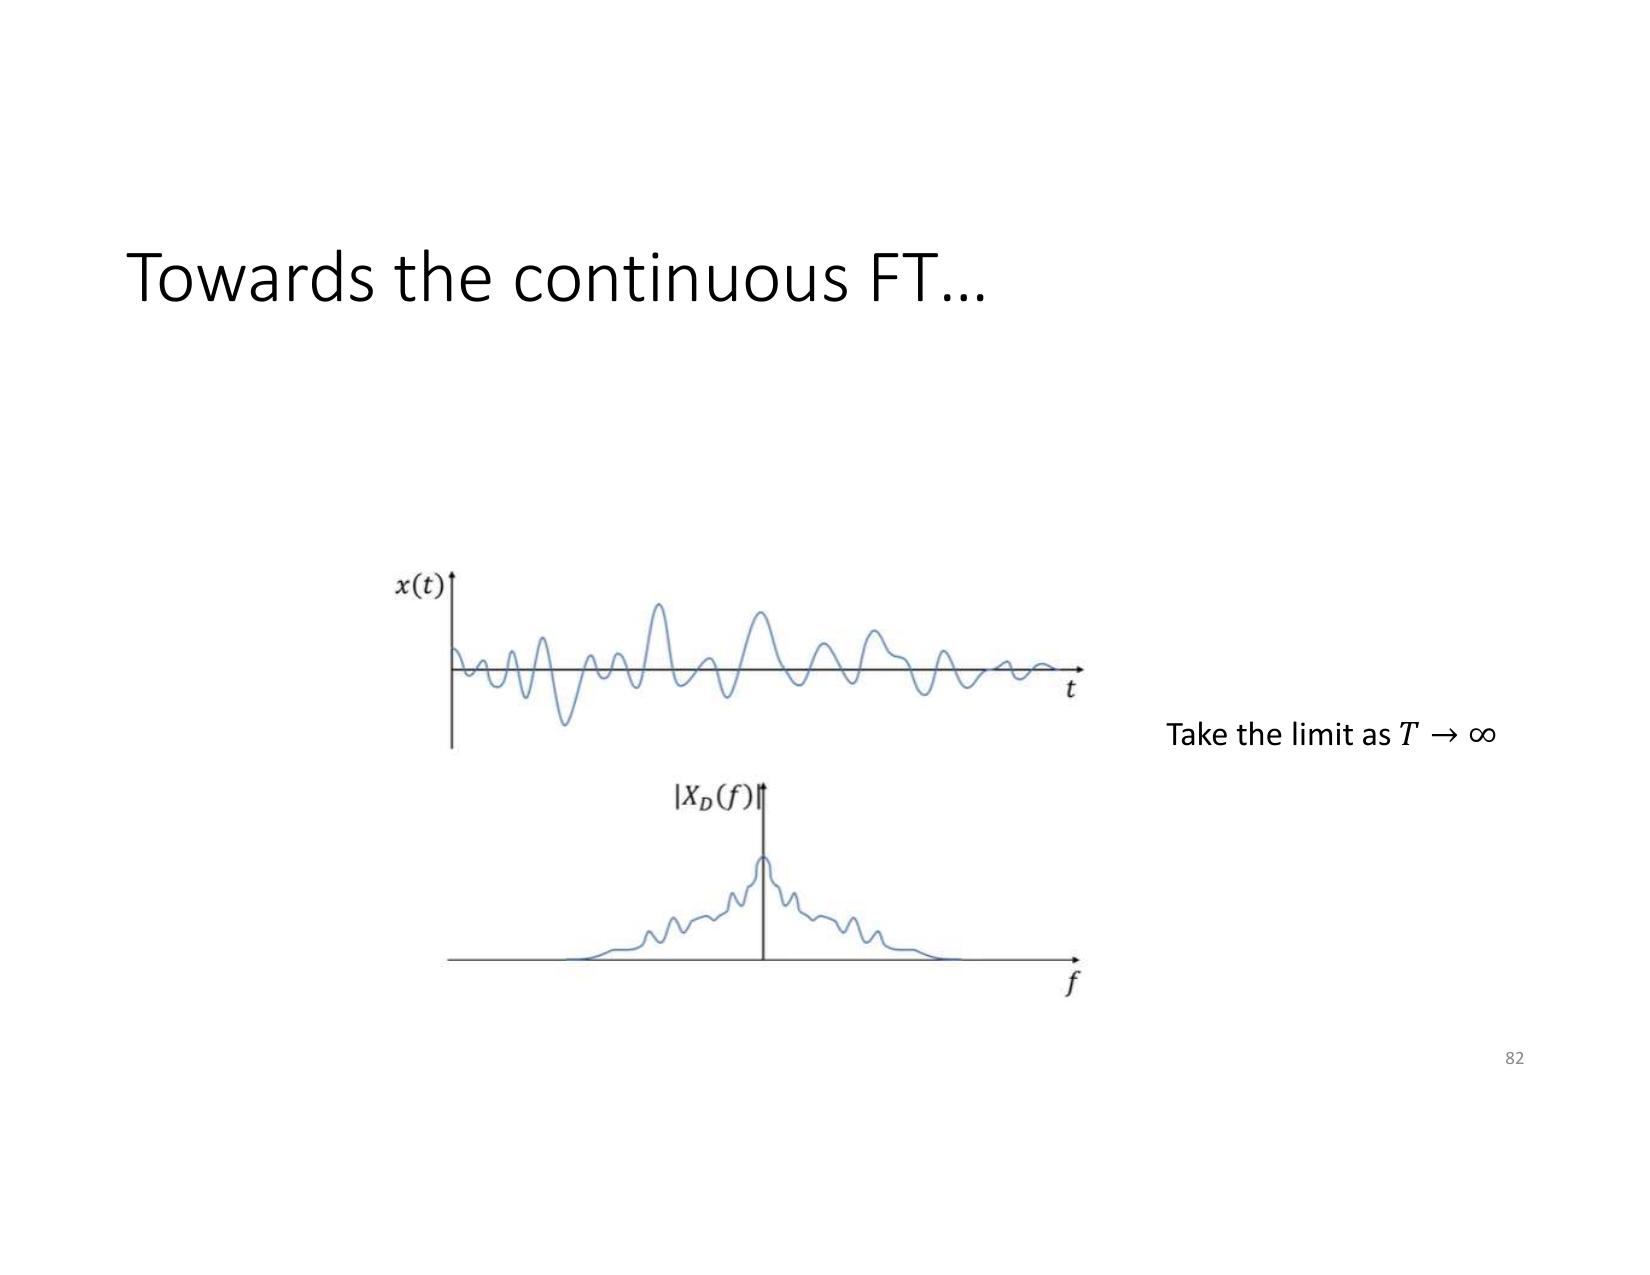
\includegraphics[keepaspectratio]{images/lezione-27-lab-teoria-dei-segnali-trasformata-di-fourier-campionamento-e-dft-img-02.jpg}}
\caption{Quando T→∞, il segnale ``dimentica'' la propria periodicità e
lo spettro \textbar X\_D(f)\textbar{} diventa una funzione continua
della frequenza.}
\end{figure}

\begin{calloutdefinition}{Trasformata Continua di Fourier (CFT)}

Un segnale non periodico \(s(t)\) può essere espresso come:

\[s(t) = \int_{-\infty}^{+\infty} S(f)\, e^{j2\pi ft}\, df\]

dove \(S(f)\) è la \textbf{densità spettrale complessa}, data dalla
trasformata diretta:

\[S(f) = \mathcal{F}(s(t)) = \int_{-\infty}^{+\infty} s(t)\, e^{-j2\pi ft}\, dt\]

Si scrive in forma compatta \(s(t) \Longleftrightarrow S(f)\).

\end{calloutdefinition}

A differenza della serie di Fourier --- che produce un insieme
\textbf{discreto} di coefficienti \(S_n\) --- la CFT produce uno spettro
\textbf{continuo} \(S(f)\) definito su tutte le frequenze reali
\(f \in (-\infty, +\infty)\).

\subsection{Esempio: Segnale Pulsato}\label{esempio-segnale-pulsato}

Consideriamo il segnale rettangolare:

\[s(t) = \begin{cases} 1 & \text{se } |t| \leq T/2 \\ 0 & \text{altrimenti} \end{cases}\]

La sua trasformata continua di Fourier si calcola analiticamente:

\[S(f) = \int_{-T/2}^{T/2} e^{-j2\pi ft}\, dt = T \cdot \text{sinc}(\pi f T) = \frac{\sin(\pi f T)}{\pi f}\]

Il risultato è una funzione \textbf{sinc} nel dominio della frequenza.
Un fatto cruciale è che all'aumentare di \(T\) (impulso più largo nel
tempo), lo spettro si restringe in frequenza, e viceversa. Questo è il
principio di \textbf{incertezza tempo-frequenza}: un segnale non può
essere contemporaneamente concentrato sia nel tempo che in frequenza.

\begin{figure}
\centering
\pandocbounded{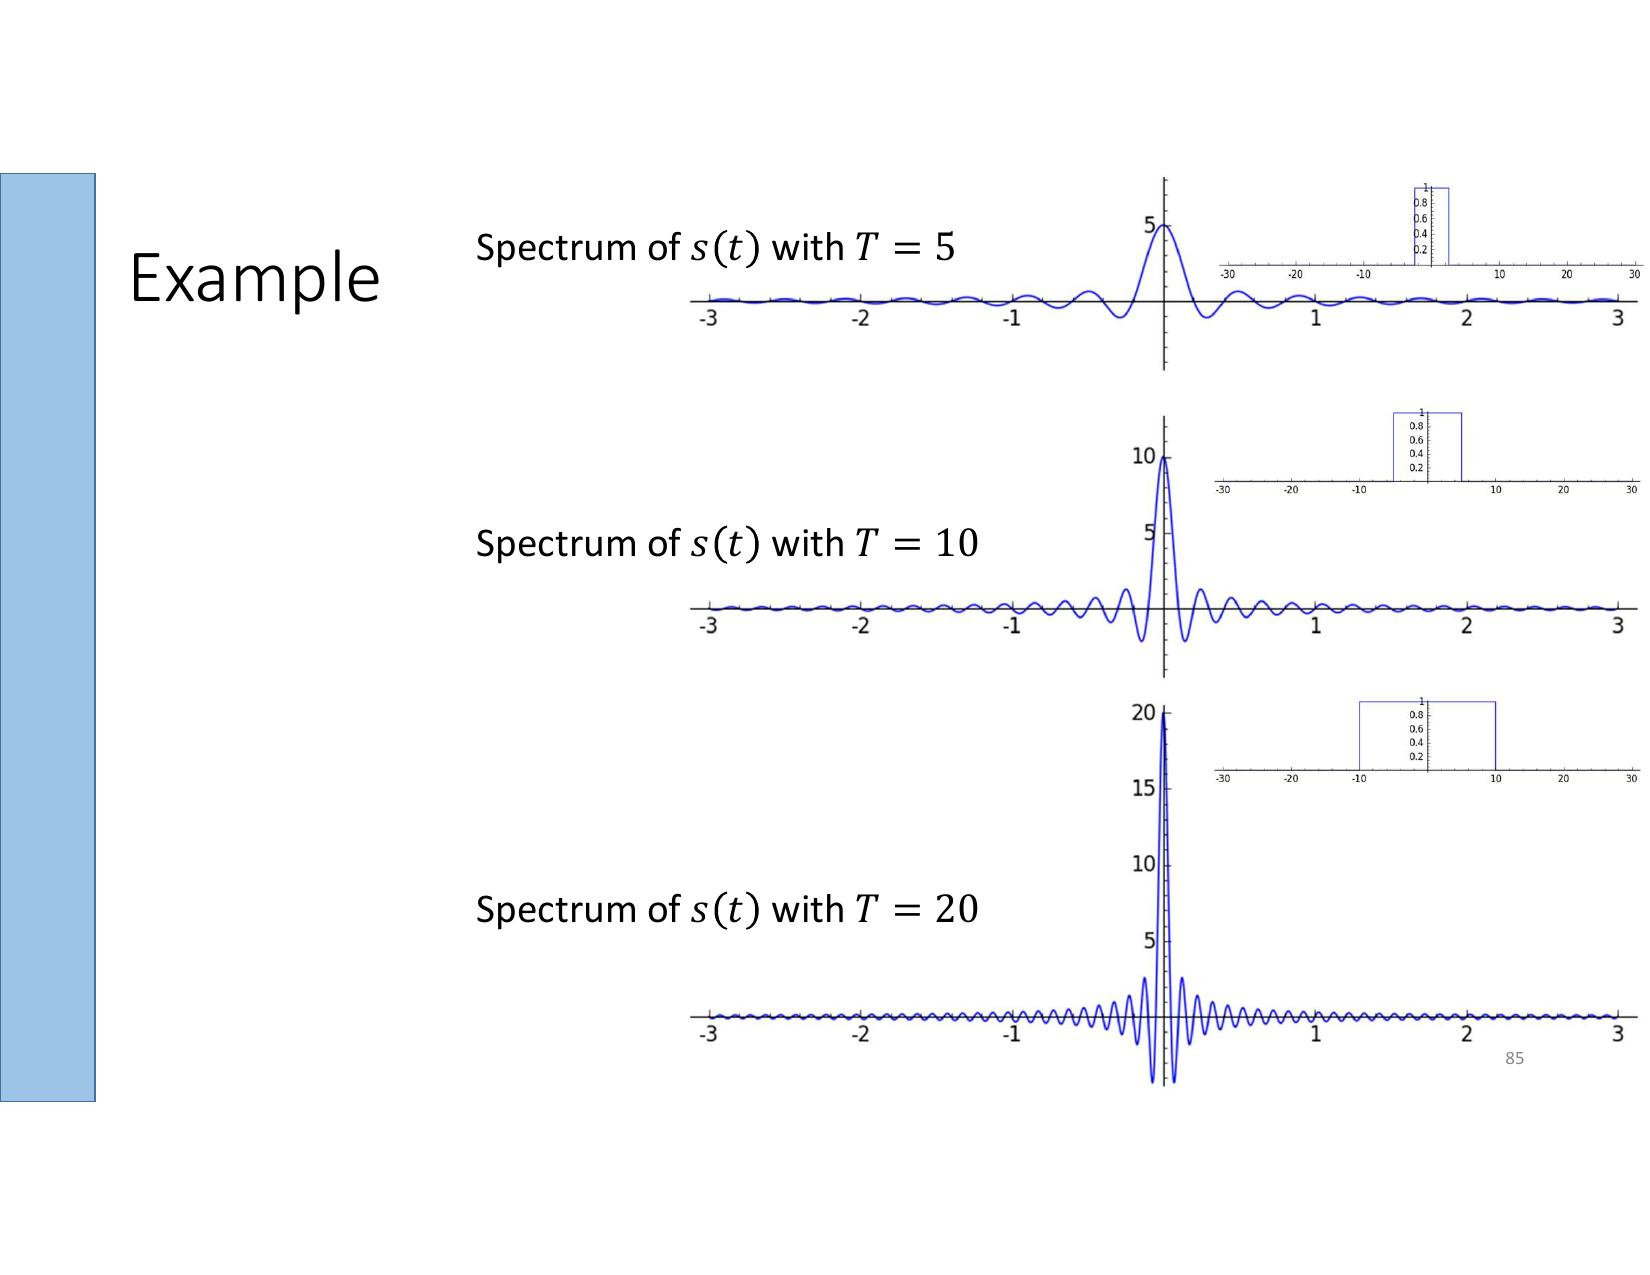
\includegraphics[keepaspectratio]{images/lezione-27-lab-teoria-dei-segnali-trasformata-di-fourier-campionamento-e-dft-img-03.jpg}}
\caption{Spettri del segnale pulsato al variare della durata T.
All'aumentare di T il lobo principale della sinc si restringe,
riflettendo il principio di incertezza tempo-frequenza.}
\end{figure}

\begin{figure}
\centering
\pandocbounded{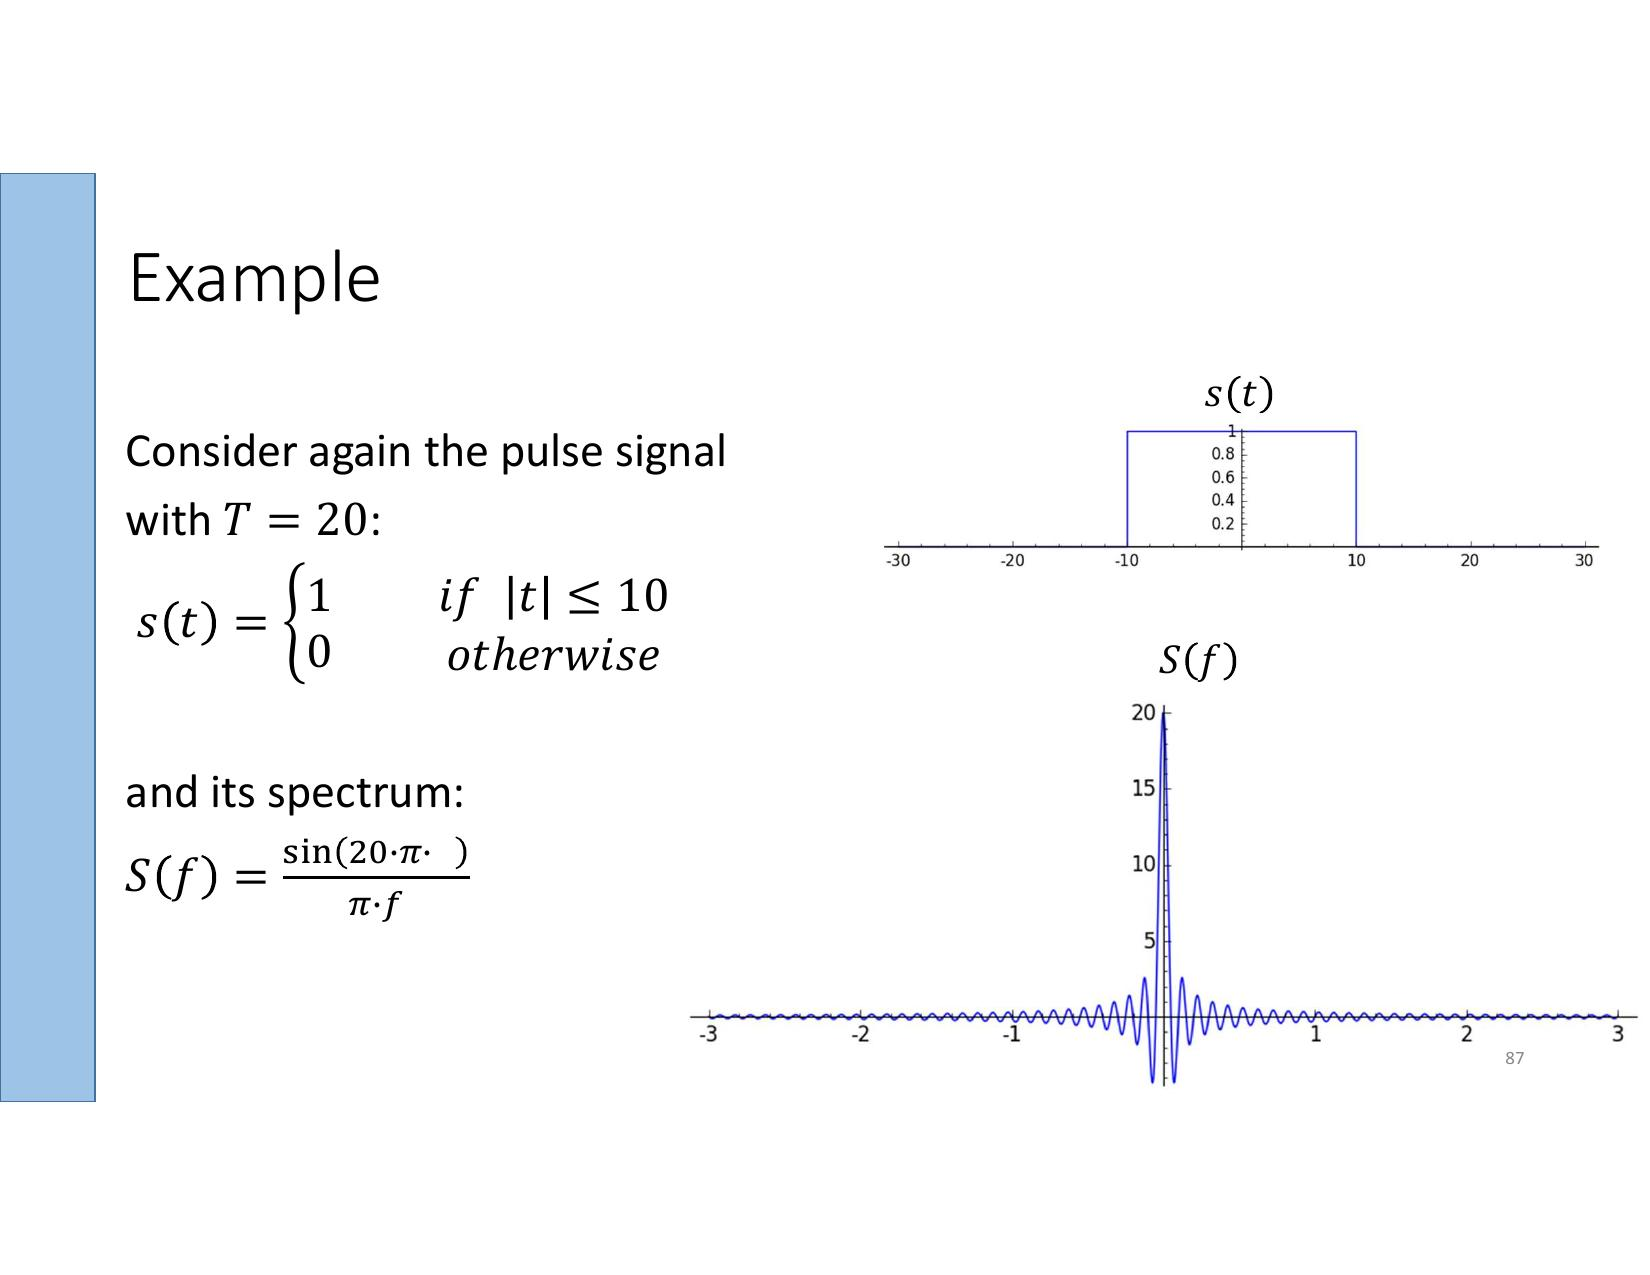
\includegraphics[keepaspectratio]{images/lezione-27-lab-teoria-dei-segnali-trasformata-di-fourier-campionamento-e-dft-img-04.jpg}}
\caption{Segnale pulsato con T=20: il segnale nel dominio del tempo
(rettangolo di ampiezza 1 e durata 20) e il corrispondente spettro
S(f)=sin(20πf)/(πf).}
\end{figure}

\subsection{Banda di un Segnale e
Filtraggio}\label{banda-di-un-segnale-e-filtraggio}

Lo spettro di un segnale generico si estende su tutte le frequenze in
\((-\infty, +\infty)\). Tuttavia, nella pratica non tutte le componenti
frequenziali sono ugualmente utili o necessarie. Filtrare un segnale
significa \textbf{selezionare un sottoinsieme delle sue componenti
spettrali}. Le motivazioni principali sono:

\begin{itemize}
\tightlist
\item
  alcune frequenze contengono l'informazione rilevante, altre
  corrispondono a rumore o interferenze
\item
  i canali di comunicazione hanno banda disponibile limitata
\item
  si vuole separare segnali che si sovrappongono in frequenza
\end{itemize}

I filtri principali sono: - \textbf{Filtro passa-basso}
(\emph{low-pass}): lascia passare le frequenze sotto una soglia \(f_c\),
blocca le alte frequenze - \textbf{Filtro passa-alto}
(\emph{high-pass}): lascia passare le frequenze sopra \(f_c\), blocca le
basse - \textbf{Filtro passa-banda} (\emph{band-pass}): lascia passare
le frequenze in un intervallo \([f_1, f_2]\)

\begin{callouttip}{Filtraggio del segnale pulsato}

Consideriamo il segnale rettangolare con \(T=20\) e il suo spettro
\(S(f) = \sin(20\pi f)/(\pi f)\).

\end{callouttip}

\begin{figure}
\centering
\pandocbounded{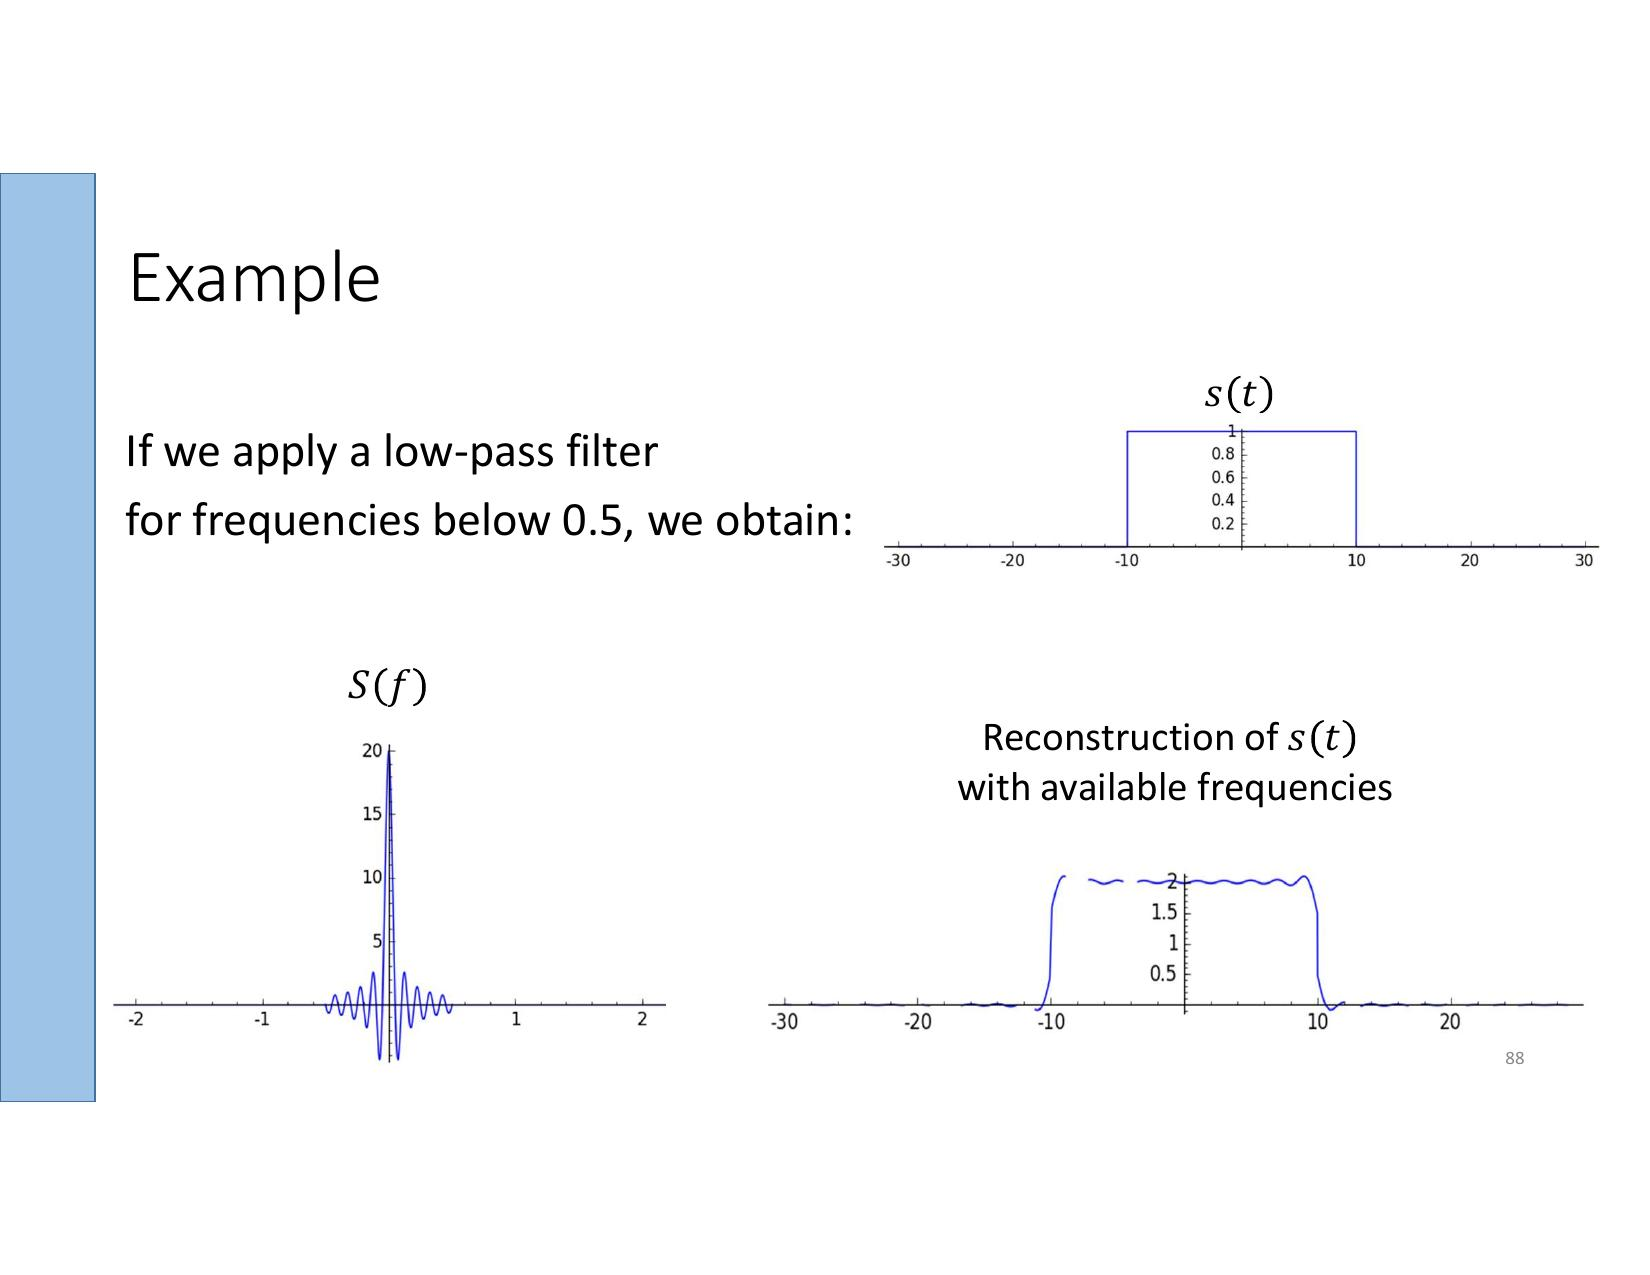
\includegraphics[keepaspectratio]{images/lezione-27-lab-teoria-dei-segnali-trasformata-di-fourier-campionamento-e-dft-img-05.jpg}}
\caption{Filtro passa-basso (soglia 0.5 Hz): lo spettro viene troncato
alle basse frequenze. La ricostruzione nel dominio del tempo riproduce
approssimativamente la forma del rettangolo, con arrotondamento agli
spigoli.}
\end{figure}

\begin{figure}
\centering
\pandocbounded{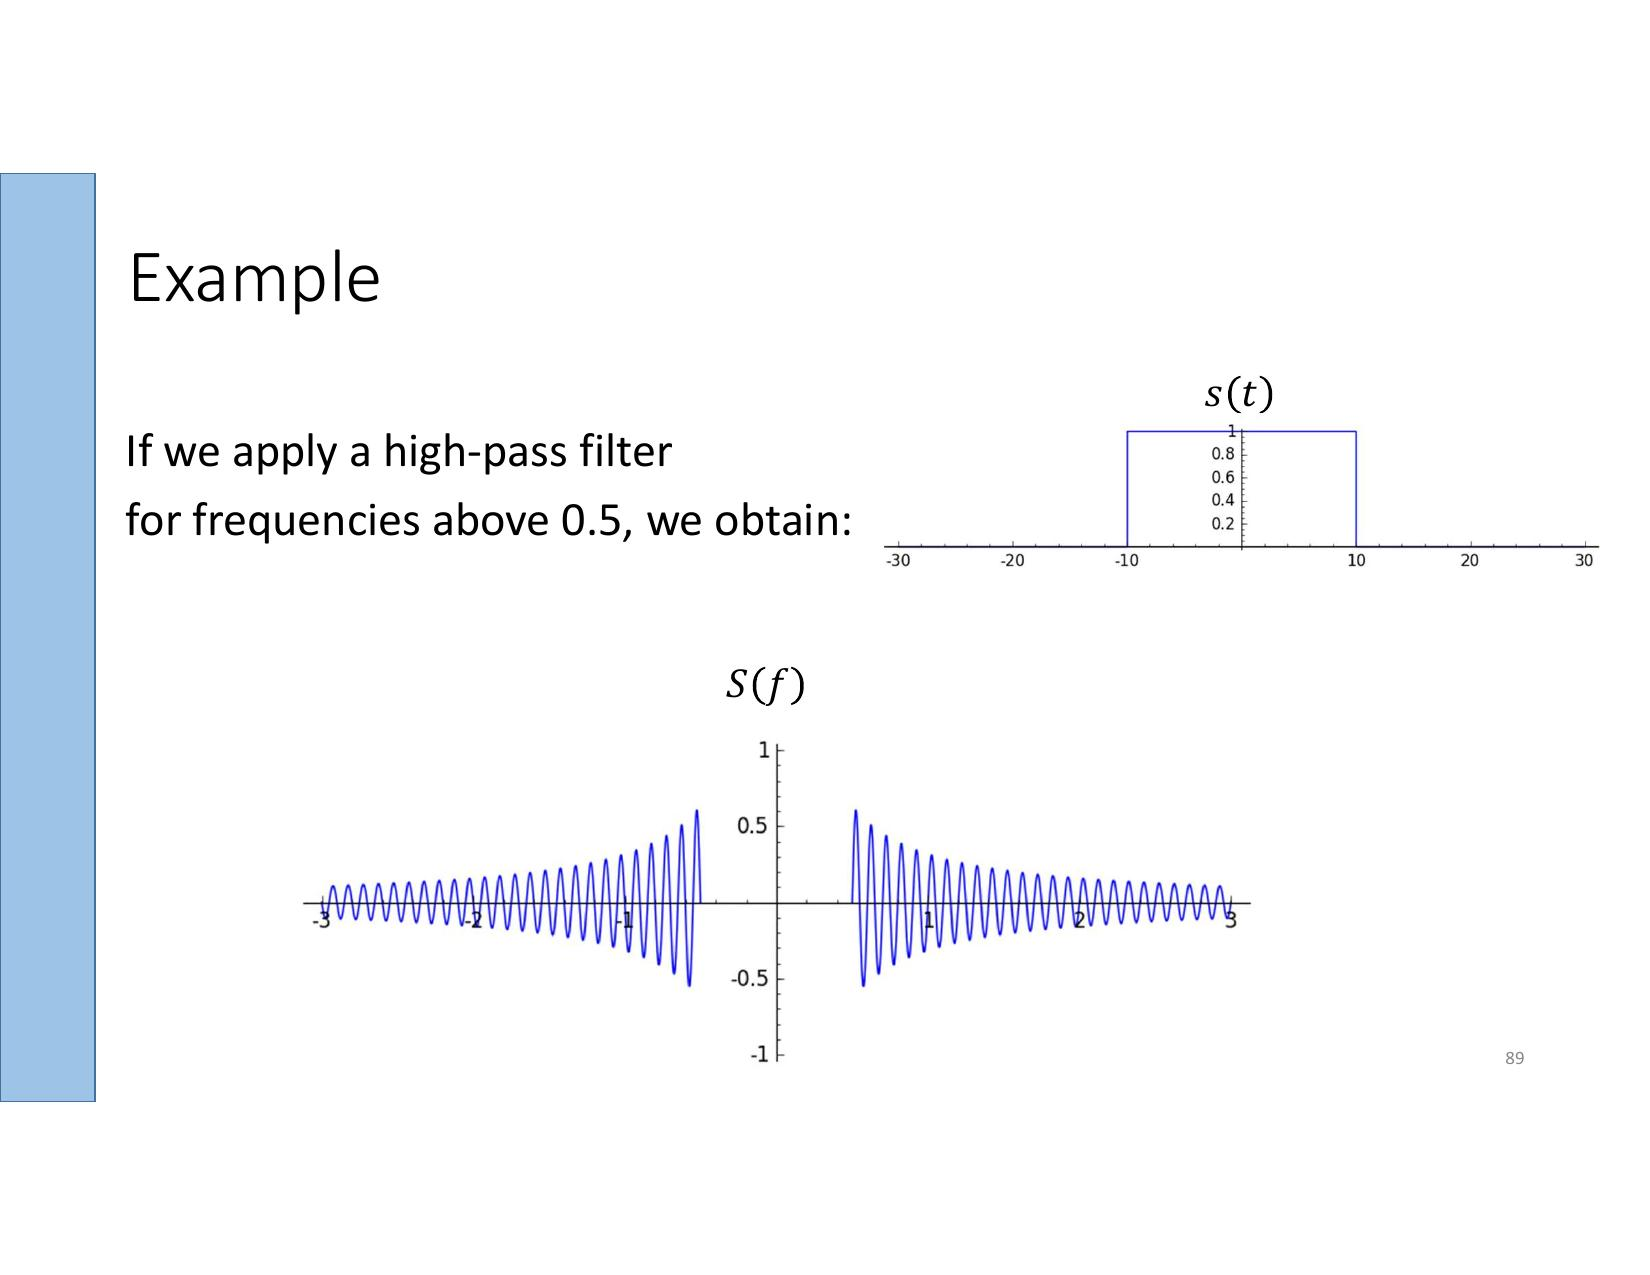
\includegraphics[keepaspectratio]{images/lezione-27-lab-teoria-dei-segnali-trasformata-di-fourier-campionamento-e-dft-img-06.jpg}}
\caption{Filtro passa-alto (soglia 0.5 Hz): rimangono solo le componenti
ad alta frequenza dello spettro. Il segnale ricostruito ha una forma
oscillatoria concentrata ai bordi del rettangolo originale.}
\end{figure}

\begin{figure}
\centering
\pandocbounded{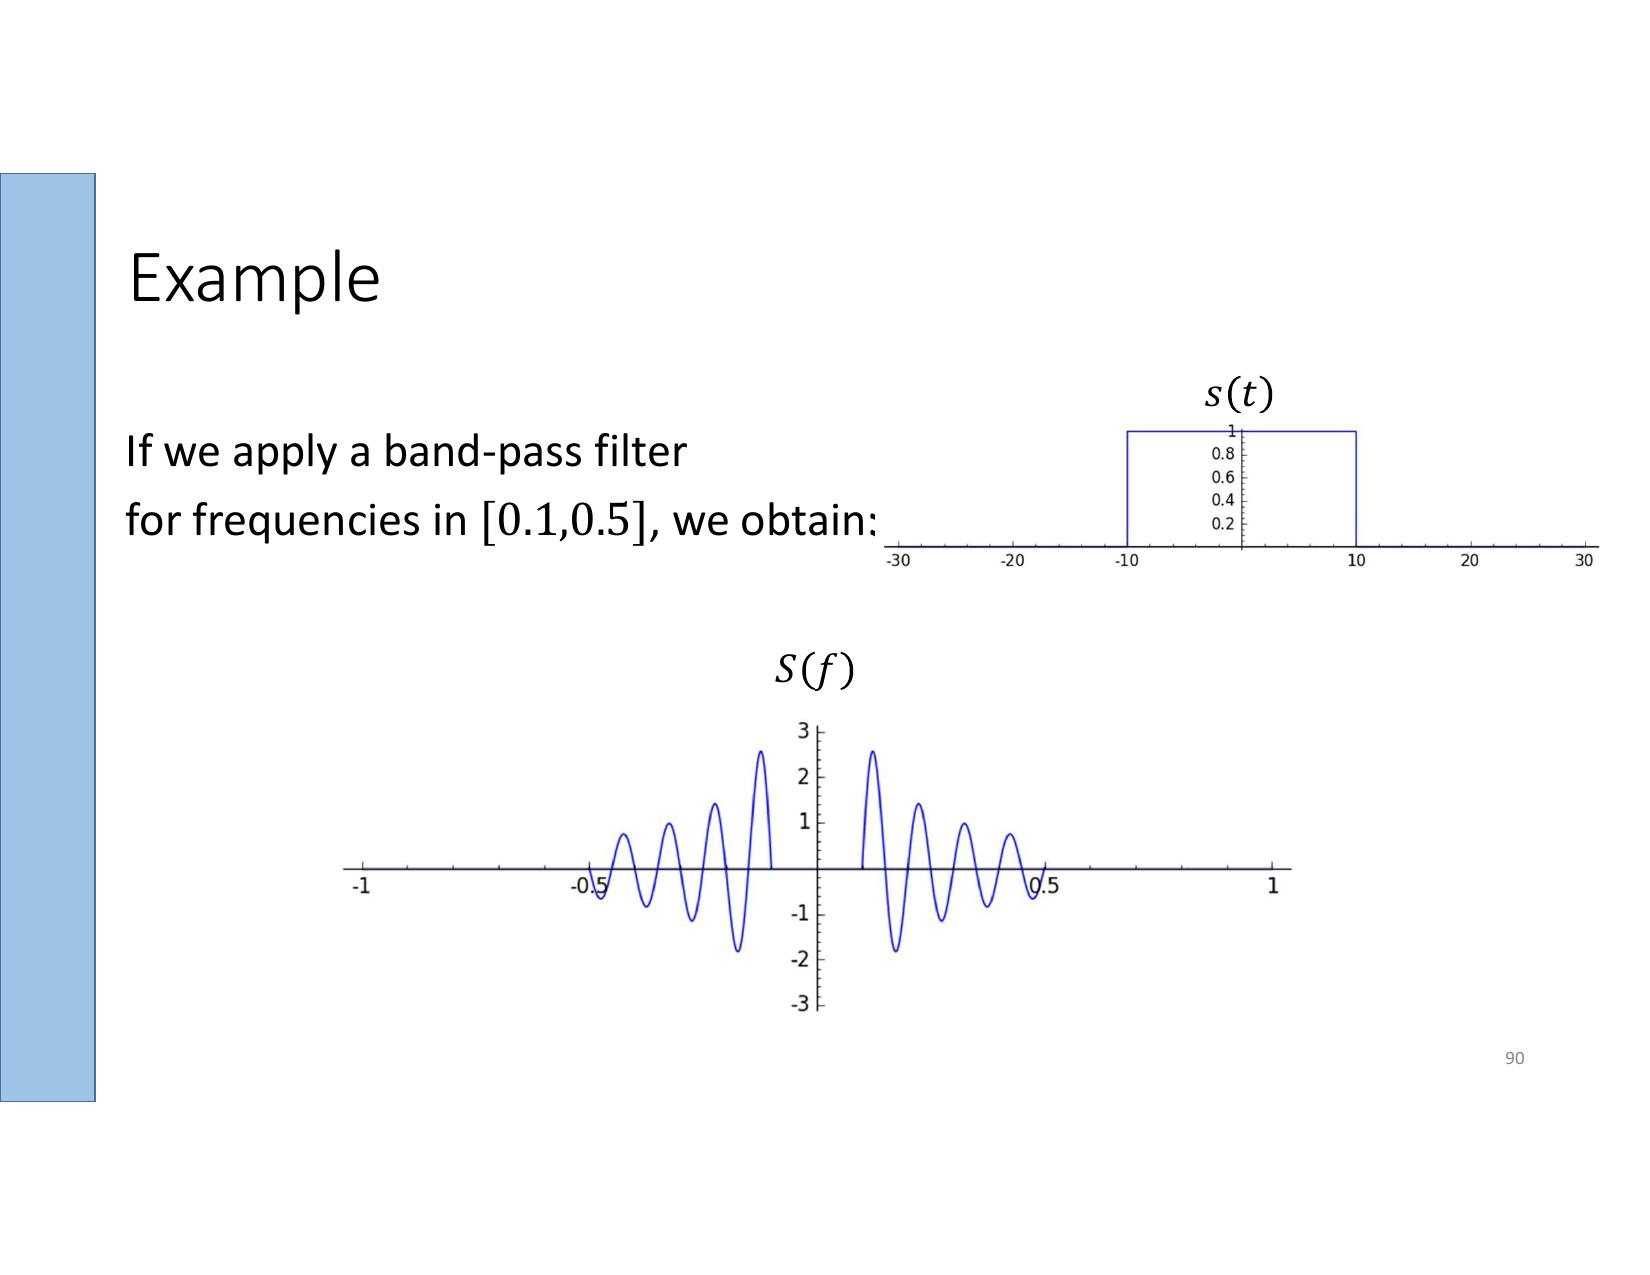
\includegraphics[keepaspectratio]{images/lezione-27-lab-teoria-dei-segnali-trasformata-di-fourier-campionamento-e-dft-img-07.jpg}}
\caption{Filtro passa-banda (intervallo {[}0.1, 0.5{]} Hz): vengono
selezionate le componenti in una fascia di frequenze. Il risultato è un
segnale oscillante.}
\end{figure}

\begin{callouttip}{Intuizione sul filtraggio}

Applicare un filtro nel dominio della frequenza equivale a moltiplicare
lo spettro \(S(f)\) per la risposta del filtro \(H(f)\). Nel dominio del
tempo questo corrisponde a una convoluzione del segnale con la risposta
impulsiva del filtro. Le basse frequenze determinano il ``contorno
grossolano'' del segnale; le alte frequenze determinano i dettagli fini
e gli spigoli.

\end{callouttip}

\subsection{Confronto: Serie di Fourier vs
Trasformata}\label{confronto-serie-di-fourier-vs-trasformata}

{\def\LTcaptype{none} % do not increment counter
\begin{longtable}[]{@{}
  >{\raggedright\arraybackslash}p{(\linewidth - 4\tabcolsep) * \real{0.3333}}
  >{\raggedright\arraybackslash}p{(\linewidth - 4\tabcolsep) * \real{0.3333}}
  >{\raggedright\arraybackslash}p{(\linewidth - 4\tabcolsep) * \real{0.3333}}@{}}
\toprule\noalign{}
\begin{minipage}[b]{\linewidth}\raggedright
\end{minipage} & \begin{minipage}[b]{\linewidth}\raggedright
Serie di Fourier
\end{minipage} & \begin{minipage}[b]{\linewidth}\raggedright
Trasformata di Fourier
\end{minipage} \\
\midrule\noalign{}
\endhead
\bottomrule\noalign{}
\endlastfoot
Tipo di segnale & Periodico & Non periodico \\
Spettro & Discreto (coefficienti \(S_n\)) & Continuo (\(S(f)\)) \\
Output & Insieme di coefficienti & Funzione continua di frequenza \\
Esempi tipici & Onda quadra, sinusoidi & Impulsi, transienti, frammenti
audio \\
\end{longtable}
}

\begin{center}\rule{0.5\linewidth}{0.5pt}\end{center}

\section{Da Segnale Analogico a Digitale: Campionamento e
Quantizzazione}\label{da-segnale-analogico-a-digitale-campionamento-e-quantizzazione}

I sistemi digitali moderni (computer, smartphone, dispositivi IoT)
lavorano esclusivamente con dati discreti. Un segnale analogico
continuo, come una voce o un sensore di temperatura, deve essere
convertito in una sequenza di valori discreti. Questo processo si
articola in due fasi: \textbf{campionamento} e \textbf{quantizzazione}.

\begin{figure}
\centering
\pandocbounded{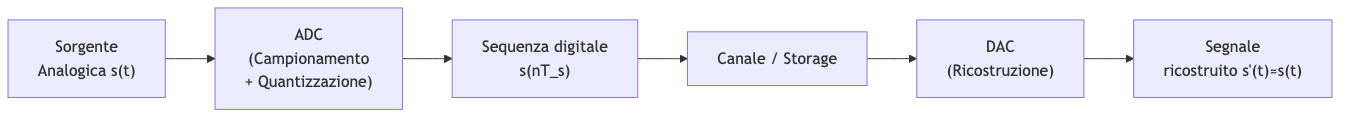
\includegraphics[keepaspectratio]{images/mermaid-lezione-27-lab-teoria-dei-segnali-trasformata-di-fourier-campionamento-e-dft-01.png}}
\caption{Pipeline di conversione analogico-digitale e
digitale-analogica. L'ADC introduce inevitabilmente un errore di
quantizzazione; il DAC ricostruisce un'approssimazione del segnale
originale.}
\end{figure}

\subsection{Campionamento}\label{campionamento}

\textbf{Campionare} un segnale \(s(t)\) significa estrarre i valori che
il segnale assume a istanti discreti regolarmente spaziati. Il parametro
chiave è il \textbf{periodo di campionamento} \(T_s\) (o
equivalentemente la \textbf{frequenza di campionamento}
\(f_s = 1/T_s\)):

\[g(nT_s) = s(nT_s), \quad n \in \mathbb{Z}\]

Il risultato è una sequenza di numeri reali. A differenza della
quantizzazione, il campionamento --- sotto opportune ipotesi --- non
introduce perdita di informazione.

\subsection{Quantizzazione}\label{quantizzazione}

Mentre il campionamento opera sull'asse del tempo, la quantizzazione
opera sull'asse dell'ampiezza: trasforma ogni campione reale
\(x \in \mathbb{R}\) in un valore intero \(y \in [0, 2^R - 1]\), dove
\(R\) è il numero di bit del quantizzatore. Si usa un
\textbf{quantizzatore scalare a \(R\) bit}:

\begin{itemize}
\tightlist
\item
  la \textbf{risoluzione} per un segnale con valori in \([0, M]\) è
  \(M / 2^R\)
\item
  il \textbf{bitrate} di una sorgente campionata a \(f_s\) e quantizzata
  a \(R\) bit è: \(B = R \cdot f_s\) bit/s
\end{itemize}

\begin{calloutwarning}{Errore di quantizzazione}

La quantizzazione introduce un errore irreversibile: due valori
analogici diversi possono essere mappati allo stesso livello digitale.
Aumentare \(R\) riduce l'errore (migliore fedeltà), ma aumenta il
bitrate da trasmettere o memorizzare.

\end{calloutwarning}

\begin{callouttip}{Sistema telefonico analogico}

La voce umana ha un contenuto informativo utile fino a circa 4 kHz
(limite telefonico accettabile). Quindi: - frequenza di campionamento:
\(f_s = 8\) kHz (doppio di 4 kHz, come vedremo con Nyquist) -
quantizzazione su \(R = 8\) bit per campione - bitrate risultante:
\(B = 8 \times 8000 = 64\) kbps

\end{callouttip}

\subsection{Interpolazione e
Ricostruzione}\label{interpolazione-e-ricostruzione}

Dato un insieme di campioni, esistono vari metodi di ricostruzione del
segnale analogico: - \textbf{Zero-order hold}: ogni campione viene
``tenuto'' fino al successivo (segnale a gradini) - \textbf{First-order
hold}: interpolazione lineare tra campioni adiacenti -
\textbf{Interpolazione con seno cardinale} (\emph{sinc interpolation}):
metodo ottimale, usato nella dimostrazione del teorema di Nyquist

\begin{center}\rule{0.5\linewidth}{0.5pt}\end{center}

\section{Il Teorema di Campionamento di
Nyquist-Shannon}\label{il-teorema-di-campionamento-di-nyquist-shannon}

La domanda centrale della conversione A/D è: \textbf{a quale frequenza
minima devo campionare per poter ricostruire perfettamente il segnale
originale?}

\begin{callouttheorem}{Teorema di Nyquist-Shannon}

Sia \(s(t)\) un segnale con spettro nullo per frequenze superiori a
\(f_M\) (segnale \textbf{a banda limitata}). Allora \(s(t)\) è
completamente determinato dai suoi campioni presi all'intervallo:

\[T_s \leq \frac{1}{2f_M}\]

ovvero con frequenza di campionamento \(f_s \geq 2f_M\). La frequenza
minima \(f_N = 2f_M\) è chiamata \textbf{frequenza di Nyquist} o
\textbf{tasso di Nyquist}.

La ricostruzione esatta si ottiene tramite interpolazione con seno
cardinale:
\[s(t) = \sum_{n=-\infty}^{+\infty} s(nT_s) \cdot \frac{\sin(\pi f_s (t - nT_s))}{\pi f_s (t - nT_s)}\]

\end{callouttheorem}

Il teorema richiede che il segnale sia \textbf{strettamente a banda
limitata} --- condizione che, come vedremo, non è mai soddisfatta dai
segnali reali.

\begin{center}\rule{0.5\linewidth}{0.5pt}\end{center}

\section{Aliasing: Il Problema del
Sottocampionamento}\label{aliasing-il-problema-del-sottocampionamento}

Per capire cosa succede quando si campiona troppo lentamente, bisogna
guardare allo spettro del segnale campionato nel dominio della
frequenza.

\subsection{FT del Segnale Campionato}\label{ft-del-segnale-campionato}

Quando si campiona un segnale \(s(t)\) con frequenza \(f_s\), la
trasformata di Fourier del segnale campionato \textbf{consiste in
infinite repliche} dello spettro originale \(S(f)\), centrate alle
frequenze multiple di \(f_s\):

\[S_c(f) = f_s \sum_{k=-\infty}^{+\infty} S(f - kf_s)\]

La spaziatura tra le repliche è pari a \(f_s\): \textbf{più veloce è il
campionamento, più distanti sono le repliche}.

\begin{figure}
\centering
\pandocbounded{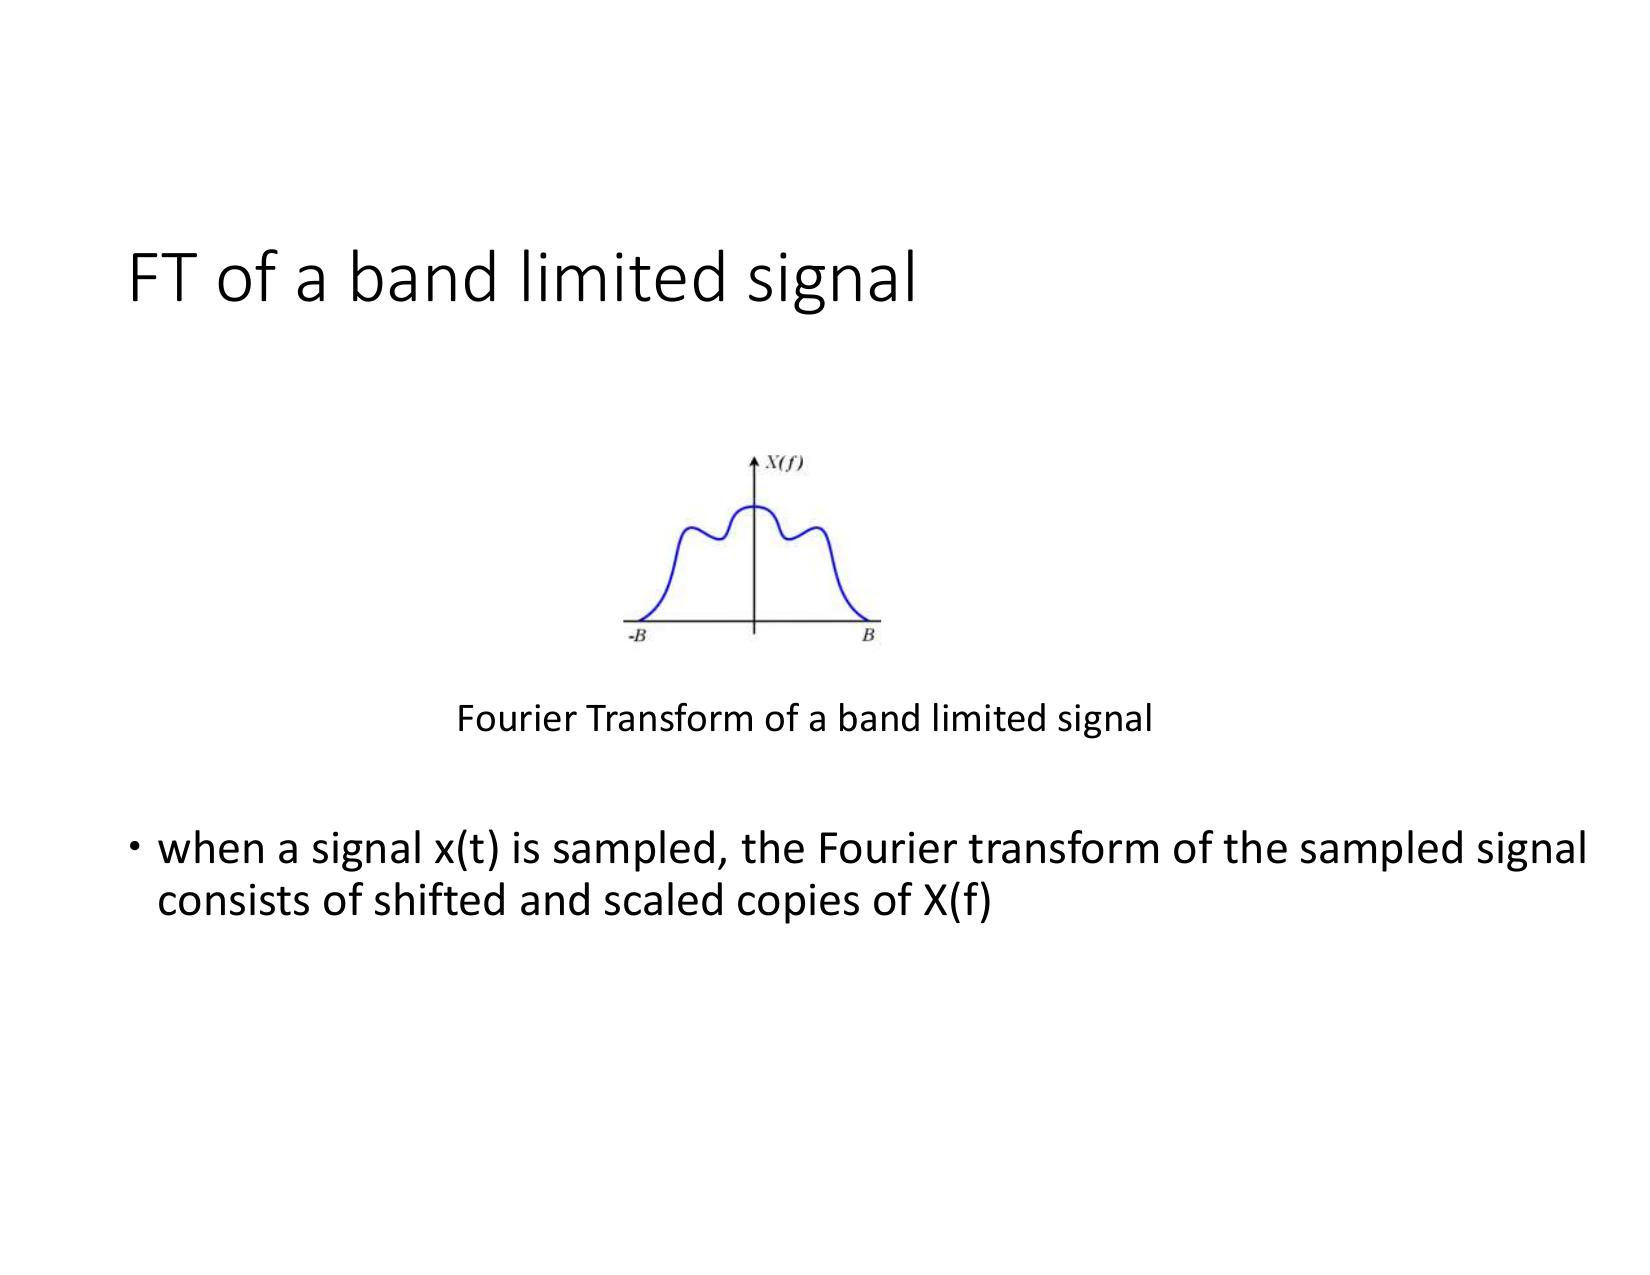
\includegraphics[keepaspectratio]{images/lezione-27-lab-teoria-dei-segnali-trasformata-di-fourier-campionamento-e-dft-img-08.jpg}}
\caption{Trasformata di Fourier di un segnale a banda limitata B. Quando
il segnale viene campionato, lo spettro si ``replica'' attorno a
multipli della frequenza di campionamento fs.}
\end{figure}

\begin{figure}
\centering
\pandocbounded{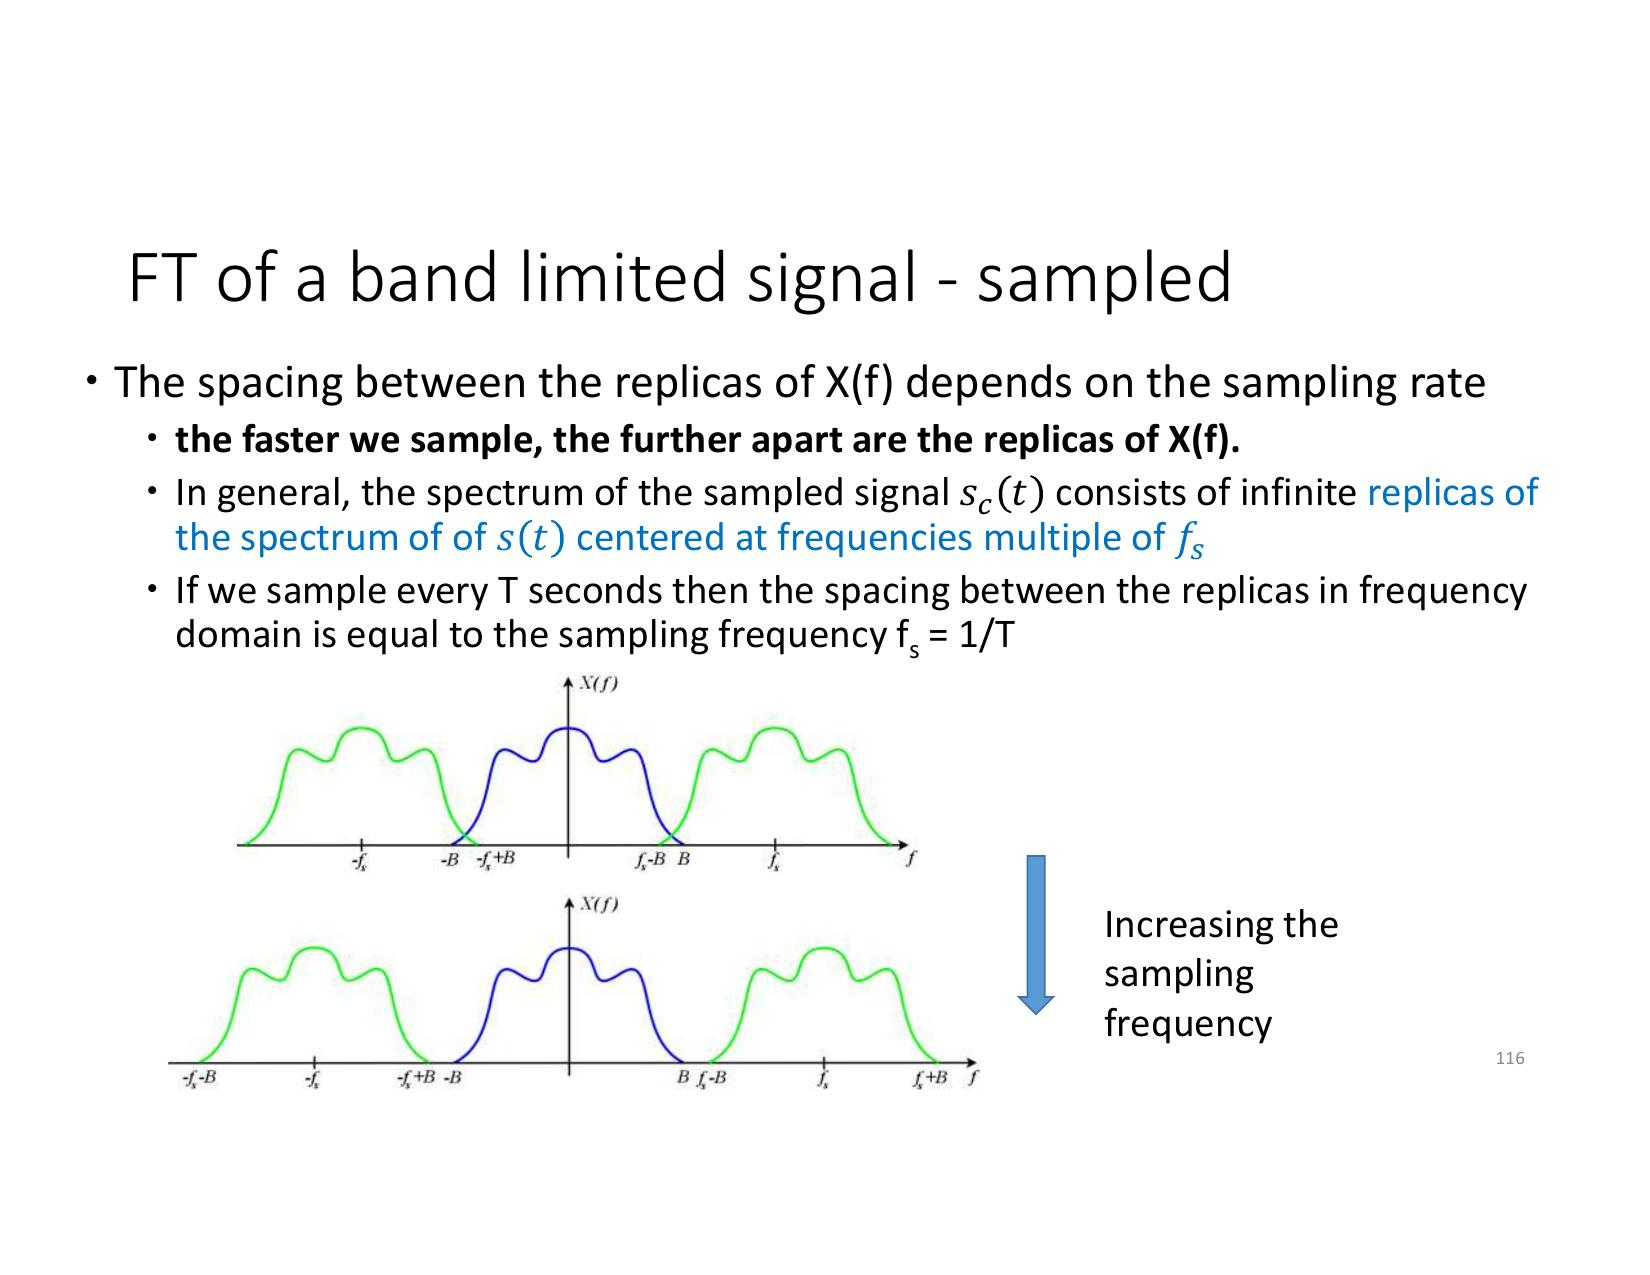
\includegraphics[keepaspectratio]{images/lezione-27-lab-teoria-dei-segnali-trasformata-di-fourier-campionamento-e-dft-img-09.jpg}}
\caption{Aumentando la frequenza di campionamento, le repliche dello
spettro si allontanano. Con campionamento sufficientemente veloce (in
basso), le repliche non si sovrappongono e il segnale originale è
recuperabile applicando un filtro passa-basso.}
\end{figure}

\begin{calloutdefinition}{Aliasing}

L'\textbf{aliasing} è la distorsione che si verifica quando le repliche
spettrali generate dal campionamento si \textbf{sovrappongono} tra loro.
Quando c'è sovrapposizione, le componenti frequenziali si mescolano e il
segnale originale non può più essere ricostruito univocamente.

\end{calloutdefinition}

\begin{figure}
\centering
\pandocbounded{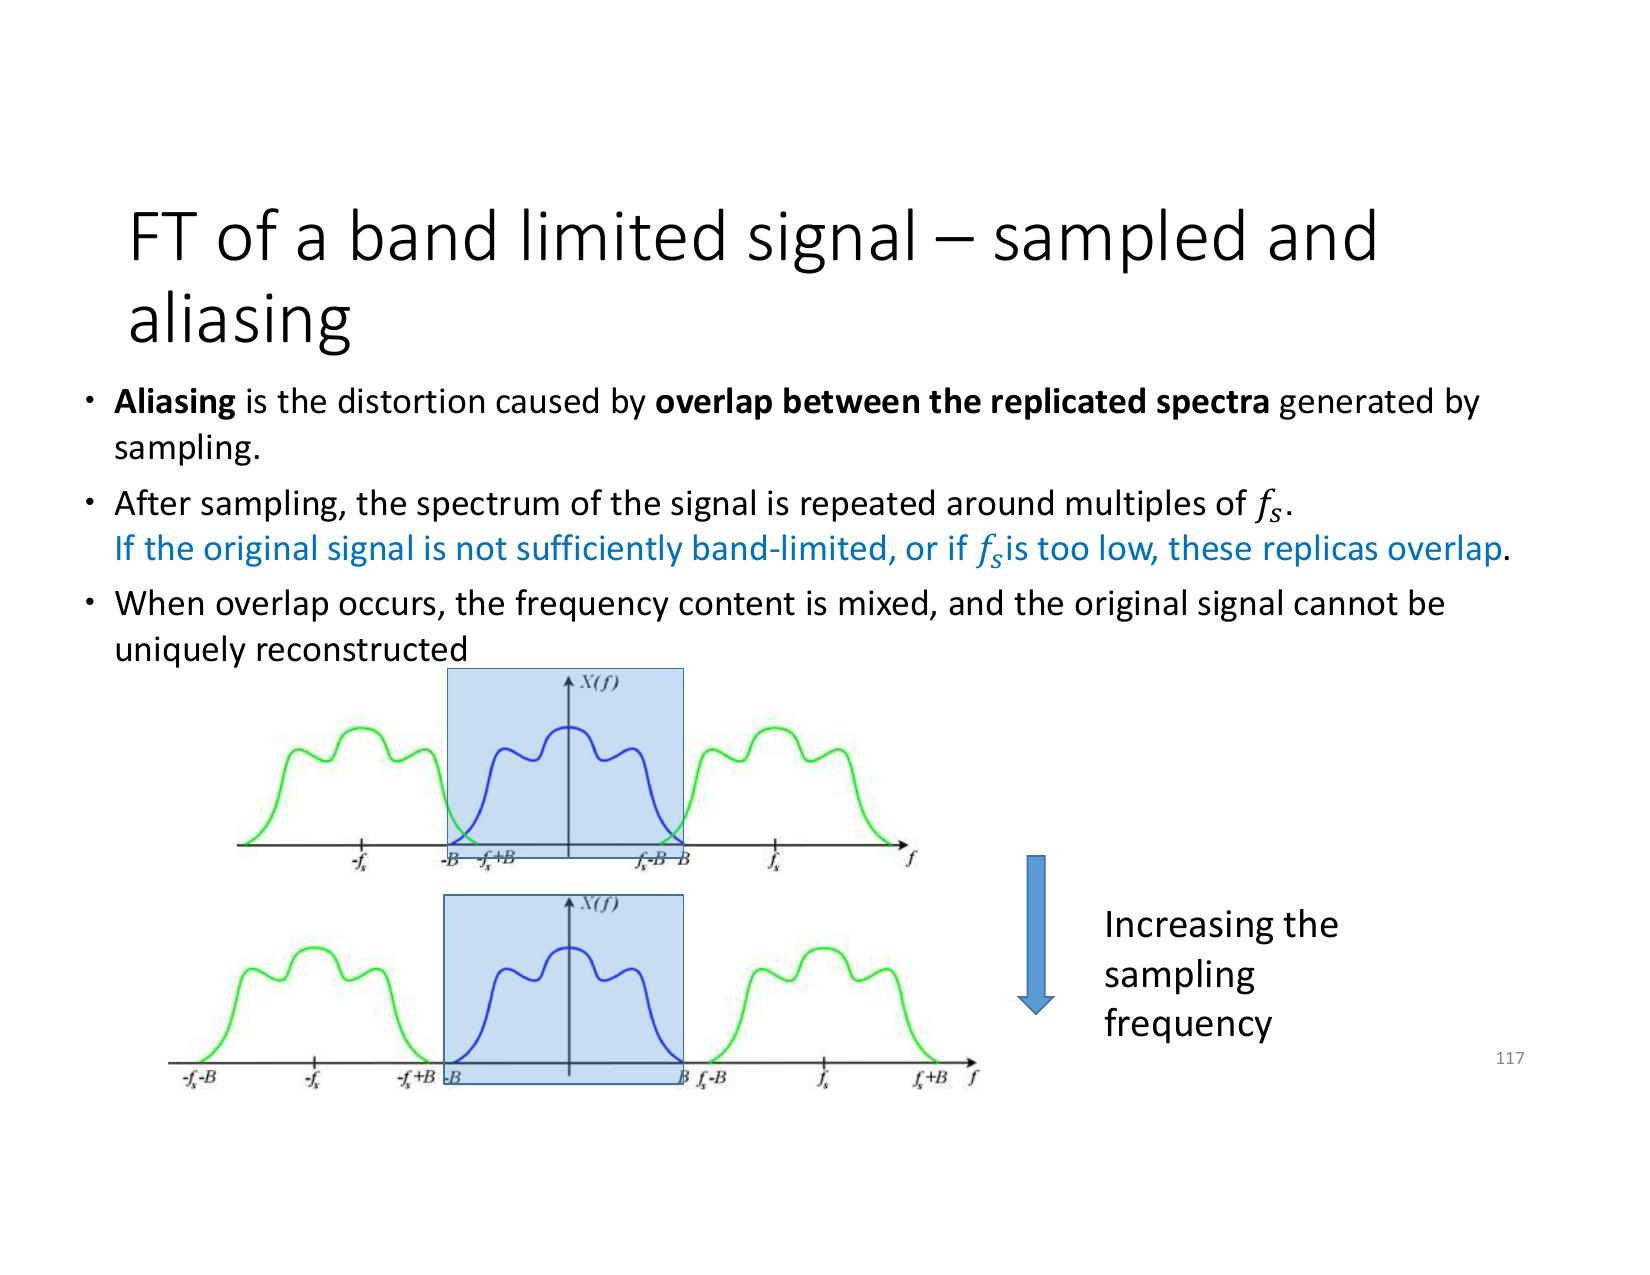
\includegraphics[keepaspectratio]{images/lezione-27-lab-teoria-dei-segnali-trasformata-di-fourier-campionamento-e-dft-img-10.jpg}}
\caption{Aliasing per frequenza di campionamento insufficiente: la
spaziatura tra repliche è minore di 2B e le code degli spettri si
sovrappongono, rendendo impossibile la ricostruzione.}
\end{figure}

La condizione di Nyquist garantisce che \textbf{non ci sia
sovrapposizione}: se \(f_s \geq 2f_M\), le repliche distano almeno
\(2B\) e possono essere separate con un filtro passa-basso ideale.

\begin{figure}
\centering
\pandocbounded{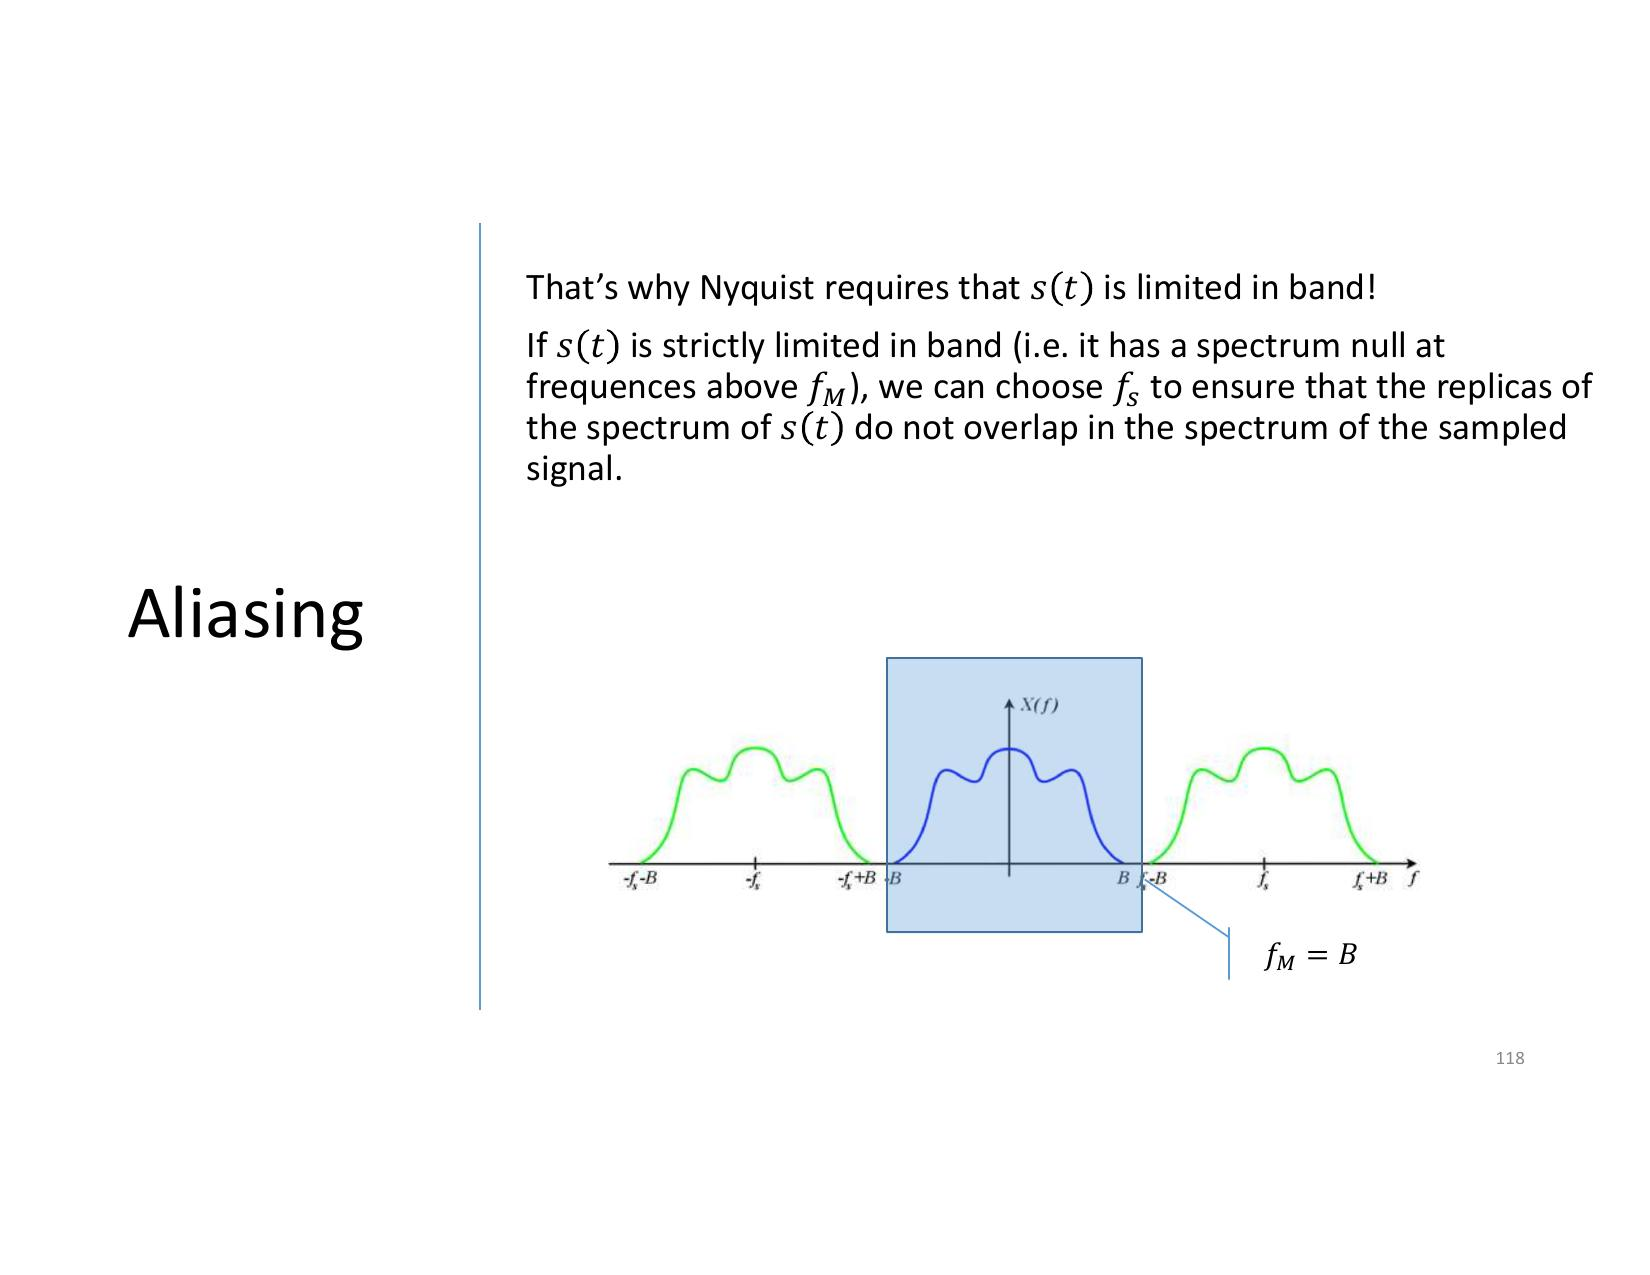
\includegraphics[keepaspectratio]{images/lezione-27-lab-teoria-dei-segnali-trasformata-di-fourier-campionamento-e-dft-img-11.jpg}}
\caption{Quando la condizione di Nyquist è soddisfatta (fs = 2B = 2fM),
le repliche dello spettro si toccano esattamente senza sovrapporsi: il
segnale originale è recuperabile con un filtro ideale.}
\end{figure}

\subsection{Cosa Nyquist Non Ha Detto}\label{cosa-nyquist-non-ha-detto}

Il teorema di Nyquist è spesso mal interpretato nella pratica. Ecco le
trappole più comuni:

\begin{calloutwarning}{Limiti pratici del teorema di Nyquist}

\begin{enumerate}
\def\labelenumi{\arabic{enumi}.}
\item
  \textbf{Nessun segnale reale è strettamente a banda limitata.} Un
  segnale a banda strettamente limitata deve estendersi infinitamente
  nel tempo, il che è fisicamente impossibile. In pratica, i segnali
  hanno uno spettro che decade ma non si azzera mai.
\item
  \textbf{Campionare a \(2f_M\) non basta se non si usa un filtro
  anti-aliasing perfetto.} I filtri reali non hanno una risposta
  rettangolare ideale: frequenze superiori a \(f_M\) passano, seppur
  attenuate. Il risultato è un aliasing residuo non trascurabile.
\item
  \textbf{La soluzione pratica è l'oversampling}: campionare a una
  frequenza significativamente superiore a \(2f_M\), e applicare un
  filtro anti-aliasing con taglio a \(f_M\) (anche se non ideale,
  l'attenuazione supplementare è sufficiente).
\end{enumerate}

\end{calloutwarning}

\begin{callouttip}{Oversampling nel telefono (old analog)}

Il telefono analogico tradizionale tagliava la voce a \textasciitilde3
kHz (non 4 kHz) e campionava a 8 kHz: non il doppio del taglio (che
sarebbe 6 kHz), ma un oversampling moderato. La differenza copre
l'imperfezione del filtro e le componenti residue tra 3 e 4 kHz.

\end{callouttip}

\begin{calloutnote}{Downsampling e segnali periodici}

Una curiosità: per segnali \textbf{strettamente periodici} e stabili, si
può addirittura \emph{sottocampionare} (\(f_s < 2f_M\)). Ogni campione
cade in una fase diversa del ciclo (perché il periodo di campionamento
non è un multiplo del periodo del segnale). Raccogliendo abbastanza
campioni nel tempo, si coprono tutte le fasi del segnale e la
ricostruzione diventa possibile. Questo funziona \textbf{solo} se il
segnale non varia nel tempo.

\end{calloutnote}

\begin{center}\rule{0.5\linewidth}{0.5pt}\end{center}

\section{Trasformata Discreta di Fourier
(DFT)}\label{trasformata-discreta-di-fourier-dft}

Nel contesto del \textbf{digital signal processing}, né la serie di
Fourier (richiede un segnale periodico continuo) né la CFT (richiede
un'integrazione continua) sono direttamente applicabili: si ha sempre un
numero finito di campioni. La \textbf{DFT} è lo strumento adatto.

\subsection{Motivazione}\label{motivazione}

Data una sequenza finita di \(N\) campioni \(s_k\) (con
\(k = 0, 1, \ldots, N-1\)), ottenuta campionando un segnale a frequenza
\(f_s\) per un tempo \(T = N/f_s\), si tratta il segnale discreto come
se fosse \textbf{periodico con periodo \(T\)} e si calcola la serie di
Fourier corrispondente. I coefficienti risultanti formano la DFT.

\subsection{Definizione della DFT}\label{definizione-della-dft}

\begin{calloutdefinition}{Trasformata Discreta di Fourier (DFT)}

Data una sequenza \(s_k\) di \(N\) valori (\(k = 0, 1, \ldots, N-1\)):

\textbf{Trasformata diretta:}
\[S_n = \sum_{k=0}^{N-1} s_k \, e^{-j2\pi nk/N}, \quad n = 0, 1, \ldots, N-1\]

\textbf{Trasformata inversa:}
\[s_k = \frac{1}{N} \sum_{n=0}^{N-1} S_n \, e^{j2\pi nk/N}\]

La frequenza del bin \(n\)-esimo è \(f_n = n \cdot \Delta f\), dove la
\textbf{risoluzione in frequenza} è:
\[\Delta f = \frac{f_s}{N} = \frac{1}{T}\]

\end{calloutdefinition}

La DFT prende in input un array di \(N\) valori e restituisce un array
di \(N\) valori complessi: entrambe le operazioni sono \textbf{somme}
(non integrali), quindi direttamente implementabili su un computer.

\begin{callouttip}{Esempio DFT}

Sequenza di 8 campioni: \(s[n] = 1\) per \(n = 0,1,2,3\) e \(s[n] = 0\)
per \(n = 4,5,6,7\).

I coefficienti DFT risultano: - \(S_0 = 4\) (componente DC) -
\(S_1 = 1 - j2.414\) - \(S_2 = 1 - j0.414\)\\
- \(S_3 = 1 + j0.414\) - \(S_4 = 1 + j2.414\) - \(S_5 = S_6 = S_7 = 0\)
(per parità)

\end{callouttip}

\begin{figure}
\centering
\pandocbounded{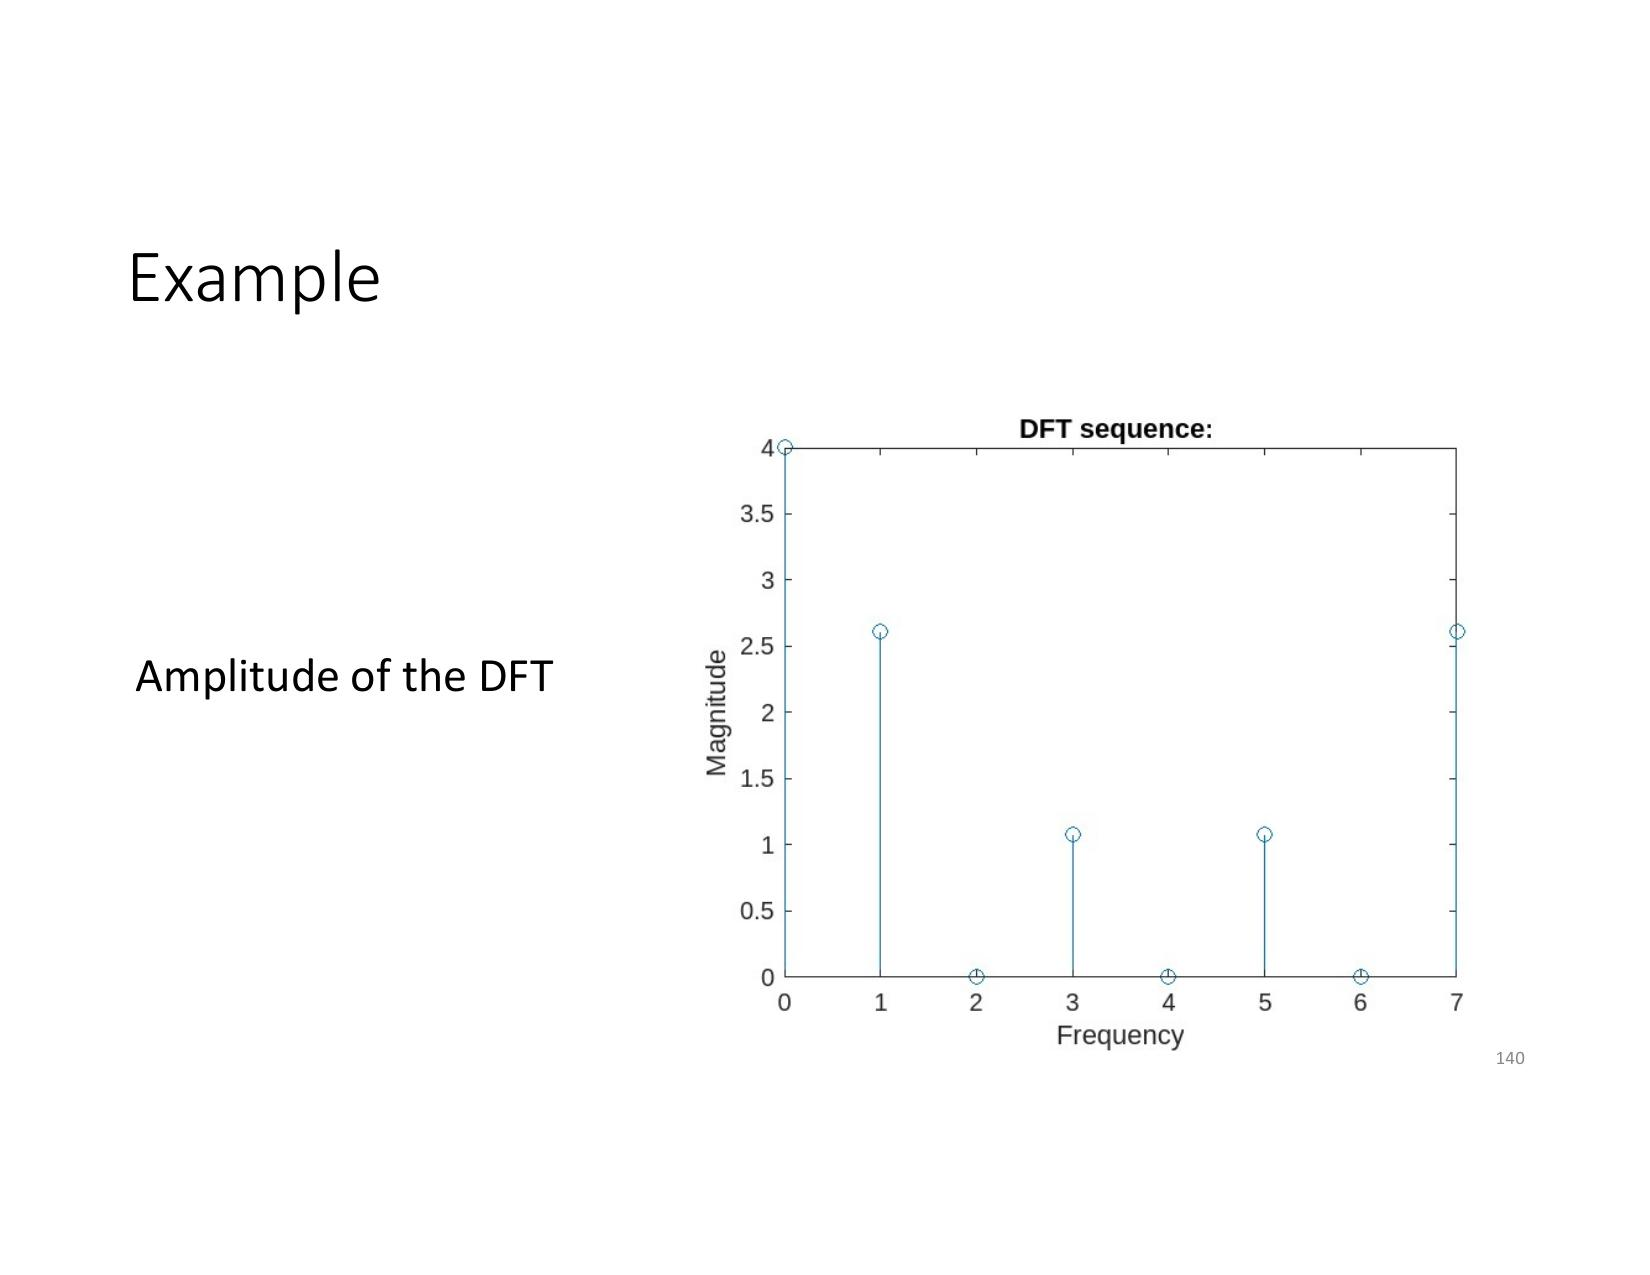
\includegraphics[keepaspectratio]{images/lezione-27-lab-teoria-dei-segnali-trasformata-di-fourier-campionamento-e-dft-img-12.jpg}}
\caption{Spettro di ampiezza \textbar S\_n\textbar{} della DFT
dell'esempio. Il valore DC (n=0) vale 4, poi i bin hanno ampiezze che
decrescono. La simmetria attorno a N/2 è caratteristica della DFT di
segnali reali.}
\end{figure}

\subsection{Fast Fourier Transform
(FFT)}\label{fast-fourier-transform-fft}

Il calcolo diretto della DFT richiede \(O(N^2)\) operazioni. Per
sequenze lunghe (audio HD: \(N = 44100\) o più), questo è proibitivo. La
\textbf{FFT} (Fast Fourier Transform) è una famiglia di algoritmi che
sfruttano la struttura periodica dell'esponenziale complesso per ridurre
la complessità a \(O(N \log N)\).

\begin{calloutnote}{Condizione sulla lunghezza}

Per la FFT più efficiente (algoritmo di Cooley-Tukey), \(N\) deve essere
una potenza di 2: \(N = 2^k\). Per questo le frequenze di campionamento
standard come 44100 Hz vengono spesso arrotondate a \(N = 32768\) o
\(65536\) campioni per la trasformazione.

\end{calloutnote}

\subsection{Commenti sulla DFT}\label{commenti-sulla-dft}

\textbf{Risoluzione in frequenza.} La DFT non ha una risoluzione
arbitraria: i ``bin'' sono spaziati di \(\Delta f = f_s / N\). Se una
componente del segnale cade tra due bin, la sua energia si spalma su più
bin adiacenti (\textbf{spectral leakage}). Per migliorare la risoluzione
si deve aumentare \(N\) (osservare il segnale più a lungo).

\textbf{Frequenza di Nyquist nella DFT.} L'analisi spettrale affidabile
tramite DFT è possibile solo per frequenze \(f < f_s/2\): le componenti
oltre la frequenza di Nyquist vengono mappate a frequenze errate
(aliasing). Filtri anti-aliasing vengono applicati prima del
campionamento per rimuovere le componenti fuori banda.

\newpage

\backmatter
\end{document}
